\documentclass[fontset=windows,11pt]{ctexart}
\usepackage{amsmath,amssymb,amsthm,mathtools}
\usepackage{geometry,booktabs,array,multirow,enumitem,longtable}
\usepackage{graphicx,xcolor}
\usepackage{placeins}
\usepackage[colorlinks=true,linkcolor=black,citecolor=black,urlcolor=blue]{hyperref}
\geometry{margin=2.2cm}
\emergencystretch=3em
\graphicspath{{figures/}}
\DeclarePairedDelimiter{\abs}{\lvert}{\rvert}
\DeclarePairedDelimiter{\norm}{\lVert}{\rVert}
\newcommand{\R}{\mathbb R}
\newcommand{\W}{W}
\newcommand{\Lop}{\mathcal L}
\newcommand{\Erem}{\mathcal E}
\newcommand{\wt}[1]{\widetilde{#1}}
\newcommand{\dd}{\,\mathrm d}
\DeclareMathOperator{\diag}{diag}
\DeclareMathOperator{\tr}{tr}
\DeclareMathOperator{\spanop}{span}
\DeclareMathOperator{\TV}{TV}
\DeclareMathOperator{\sech}{sech}
\newtheorem{assumption}{假设}[section]
\newtheorem{definition}{定义}[section]
\newtheorem{lemma}{引理}[section]
\newtheorem{proposition}{命题}[section]
\newtheorem{theorem}{定理}[section]
\newtheorem{corollary}{推论}[section]
\newtheorem{example}{例}[section]
\newtheorem*{remark}{注记}
\numberwithin{equation}{section}
\newcommand{\expclaim}[1]{\textcolor{teal!60!black}{[经验~$n={#1}$]}}

\title{\textbf{空间加权在 PINN 中能改变什么、不能改变什么：\\局部对角权的谱能力边界与受控证伪}\\[3pt]
\large ——粘性 Burgers 激波捕捉中的保解不变性、条件数边界与盆地选择检验}
\author{温宁\\[2pt]
\small 独立研究者\\[1pt]
\small \href{mailto:wenning-compmath@outlook.com}{wenning-compmath@outlook.com}\\[1pt]
\small \href{https://orcid.org/0009-0005-5395-7791}{ORCID: 0009-0005-5395-7791}}
\date{}

\begin{document}
\maketitle
\begin{abstract}

物理信息神经网络（PINN）在刚性问题上常收敛到伪解，空间加权是最常见的干预手段之一。本文围绕一个问题展开：对加权训练目标 $L_\W=\tfrac{1}{2N} r^\top \W r$（经验平均口径、冻结或外生缓变权重），改变空间对角权重 $\W$ 究竟作用在哪些数学对象上、各自的因果链是什么。为组织分析，本文按 Taylor 展开阶数将加权作用区分为零阶（解/适定性）、一阶（梯度/优化动力学）与二阶（冻结线性化谱）三个层面。

本文给出三类能力边界：（1）二阶层面上，空间局部对角加权保持冻结 Gram 的相关矩阵严格不变，只能缩放特征值尺度、且缩放幅度受有界带约束（van der Sluis 带），等相关阵上条件数已最优；唯一能白化的非局部权 $\W\propto K_r^{-1}$ 稠密且 $O(N^3)$，在线训练不可行。实验 4.2 在真实 Burgers 冻结 Jacobian 上严格静态验证：多起点 L-BFGS-B\emph{找到}的改善在 $N\le512$ 为 13\%--24\%、$N=1024$ 时 $\kappa(R)\gtrsim10^{13}$ 近双精度极限、未纳入定量结论，真实最优改善不低于此值（优化值为上界），改善上限受 van der Sluis 带 $r\ge1/N$ 约束，不能白化由定理代数保证。实验 4.3 作为训练过程经验旁证：默认裁剪配置下减权族恶化 $1.7$--$4.9$ 倍、小粘性档 $3.0$--$4.9$ 倍，裁剪关闭时区间更宽（$0.6$--$3.4$）且个别格出现改善；该实验测完整 Hessian 而非冻结 $H_{\rm lin}$。

（2）一阶层面上，在本文研究的六族权重、$n=80$ 配对实验下未观察到加权能显著改善盆地进入概率（uniform 命中率 $.613$ 反高于全部加权族，Holm 校正后仅 down\_lin 显著 $p=.006$）；加权的可观测效应局限于已进入盆地内的收敛速度调节，减权以梯度尺度调节为主（Adam 归一化吸收后残余方向效应小，实验 5.8 检出 down\_lin 有效 lr 上限提升一倍，精确双侧 $p=.0625$（渐近 $\approx.043$），方向一致但未达 $.05$ 显著）：尺度非瓶颈时仅表现为训练早期稳定，频谱失配时可带来终态收益（跨方程验证）。事后最优 $\beta$ 是描述性观察（单种子散布 $1$--$100$），不构成可预训练部署的固定策略。

（3）无真解部署时，固定单投影标量（残差/损失自评估）的盆地判别受 Bayes 误差下界限制，四点 XOR 反例表明不可精确线性分离（最小错误 $1/4$），必须引入交互/非线性特征。携带空间对比度结构的量 $g_{et}$ 提供盆地判别可行性证据（proxy AUC $.971$，含标签—特征同源相关；oracle AUC $.64$），是有噪声判别器，价值在于过滤明显坏盆地、减少无效精修，非精确识别好盆地。实验以一维稳态粘性 Burgers 激波为主 testbed，以 Poisson 光滑退化与内部奇性原型为跨方程验证，所有结论均标注确定性、以概率 $1-\delta$ 或经验 $n=$ 三级陈述级别。

\end{abstract}

\noindent\textbf{关键词：}物理信息神经网络（PINN）；空间加权；条件数；相关矩阵不变量；吸引盆地；粘性 Burgers 方程；伪解


\section{引言}\label{sec:intro}

\subsection{研究背景与问题}\label{sec:bg}
物理信息神经网络（physics-informed neural network，PINN）把偏微分方程（PDE）残差与初边值条件以软约束并入损失函数，以全连接网络逼近解，在正、逆问题上均有广泛应用\cite{Raissi2019,Karniadakis2021,Cuomo2022}。当解光滑、算子良态时，该方法稳健；但在对流占优、含薄边界层或激波的\emph{刚性}问题上，PINN 常表现为训练损失停滞、收敛到违背物理的伪解，或对初始化高度敏感。已有研究从不同侧面给出解释：刚性导致不同项之间的梯度量级失配\cite{WangTeng2020}；在神经正切核（neural tangent kernel，NTK）视角下，不同损失分量的收敛率由相应核特征值决定、彼此失配\cite{Jacot2018,Wang2020NTK}；软约束权重不当与错误的优化曲率会系统性诱发失败模式\cite{Krishnapriyan2021}；网络的谱偏差又使其优先学习低频成分\cite{Rahaman2019,Tancik2020}。

\emph{空间加权}——按配点的空间位置对残差赋以不同权重——是应对上述困难最直接、也最常见的一类干预。它在文献中沿多条看似矛盾的路线发展：在残差大的"硬区"增大权重（硬区增权、自适应配点（RAR/RAD 类\cite{Wu2022,Nabian2021}，属类外自适应采样）、因果训练\cite{Wang2022causal}）；或反其道在间断、硬区处\emph{减弱}损失权重或网络表达\cite{Liu2022down,LessEmphasis2022}；亦有在梯度冲突层面做冲突消除（以正交投影为手段）的工作\cite{ConFIG2025}。这些方法在各自算例上有效，但其作用层面并不相同。文献中因此常见三类彼此混淆的论断：(a)~以加权后零阶解集不变为由，声称优化过程被改善；(b)~以冻结 Hessian/NTK 谱的变化，直接推断训练轨迹被改善；(c)~把训练早期梯度幅度的下降解释为"逃出错误吸引盆地"。若不在概念上区分这些层面，便无法判断某一加权策略在何种条件下有效、其收益与代价的边界何在。

\subsection{贯穿性问题与分析层面的区分}\label{sec:q}
上节三类混淆论断的共同根源，是缺少对加权作用对象的因果定位。本文的贯穿性问题因此是：对加权训练目标 $L_{\W}=\tfrac{1}{2N} r^\top \W r$（经验平均口径，$\W$ 为空间对角权重），改变 $\W$ 究竟作用在哪些数学对象上、各自的因果链是什么。为组织分析，我们按 Taylor 展开阶数将这些对象区分为三个层面（图~\ref{fig:box}）；该区分仅用于避免跨层结论互证，不构成独立的理论贡献。其一是\emph{零阶层面}：零残差解集与适定性、残差到误差的稳定性桥，在 $w>0$ 时不随 $\W$ 改变。其二是\emph{一阶层面}：加权梯度场 $g_{\W}=J^\top\W r$、由其诱导的迭代轨迹及驻点/吸引盆地（吸引域，basin of attraction，即优化迭代收敛到同一驻点的初值集合，全文简称"盆地"；收敛到伪解者称伪解吸引域，可精修到真解者称可精修吸引域）等全局几何；在一大类一阶优化算法中，$\W$ 进入\emph{单步}参数更新的唯一微分途径即加权梯度 $g_{\W}$（基于标量损失 $L_\W$ 的线搜在类外，见~\ref{sec:admit}）。其三是\emph{二阶层面}（冻结线性化谱）$H_{\rm lin}=J^\top\W J$ 及其谱：它是当前点的线性化切面，仅经梯度多步演化间接起作用；真实 Hessian 的不定性则来自残差曲率 $H_{\rm nl}=\sum_i w_i r_i\nabla_\theta^2 r_i$，它在残差趋零时消失。$H_{\rm nl}$、三阶及以上泰勒项、训练窗内的曲率漂移、预条件时变与外生跳变，统一归为\emph{受控余项}（一类有显式界的残差桶）。在时间维度上，训练分为两阶段：\emph{Phase~0（盆地选择）}在 $\beta=1$ 下借助表示课程与多起点选择进入正确盆地，\emph{Gate（关卡）}在不使用真解的条件下做一次性策略分流，\emph{Phase~1（盆地内精修）}在已进入的可精修盆地内调节增权强度 $\beta$ 完成局部收敛。实验上，全文以一维稳态粘性 Burgers 激波为主 testbed，以 Poisson 光滑退化、内部奇性原型、一维时变 Burgers 与二维线性对流—扩散为跨方程验证。这一区分直接给出可检验的判断：例如"加权改善冻结条件数"与"加权加速收敛"是二阶与一阶两个不同命题——前者对空间局部加权一般不成立，后者只在特定的盆地内条件下成立，二者不可互证。第~\ref{sec:framework} 章给出上述记号与定义的严格形式化。

\begin{figure}[ht]\centering
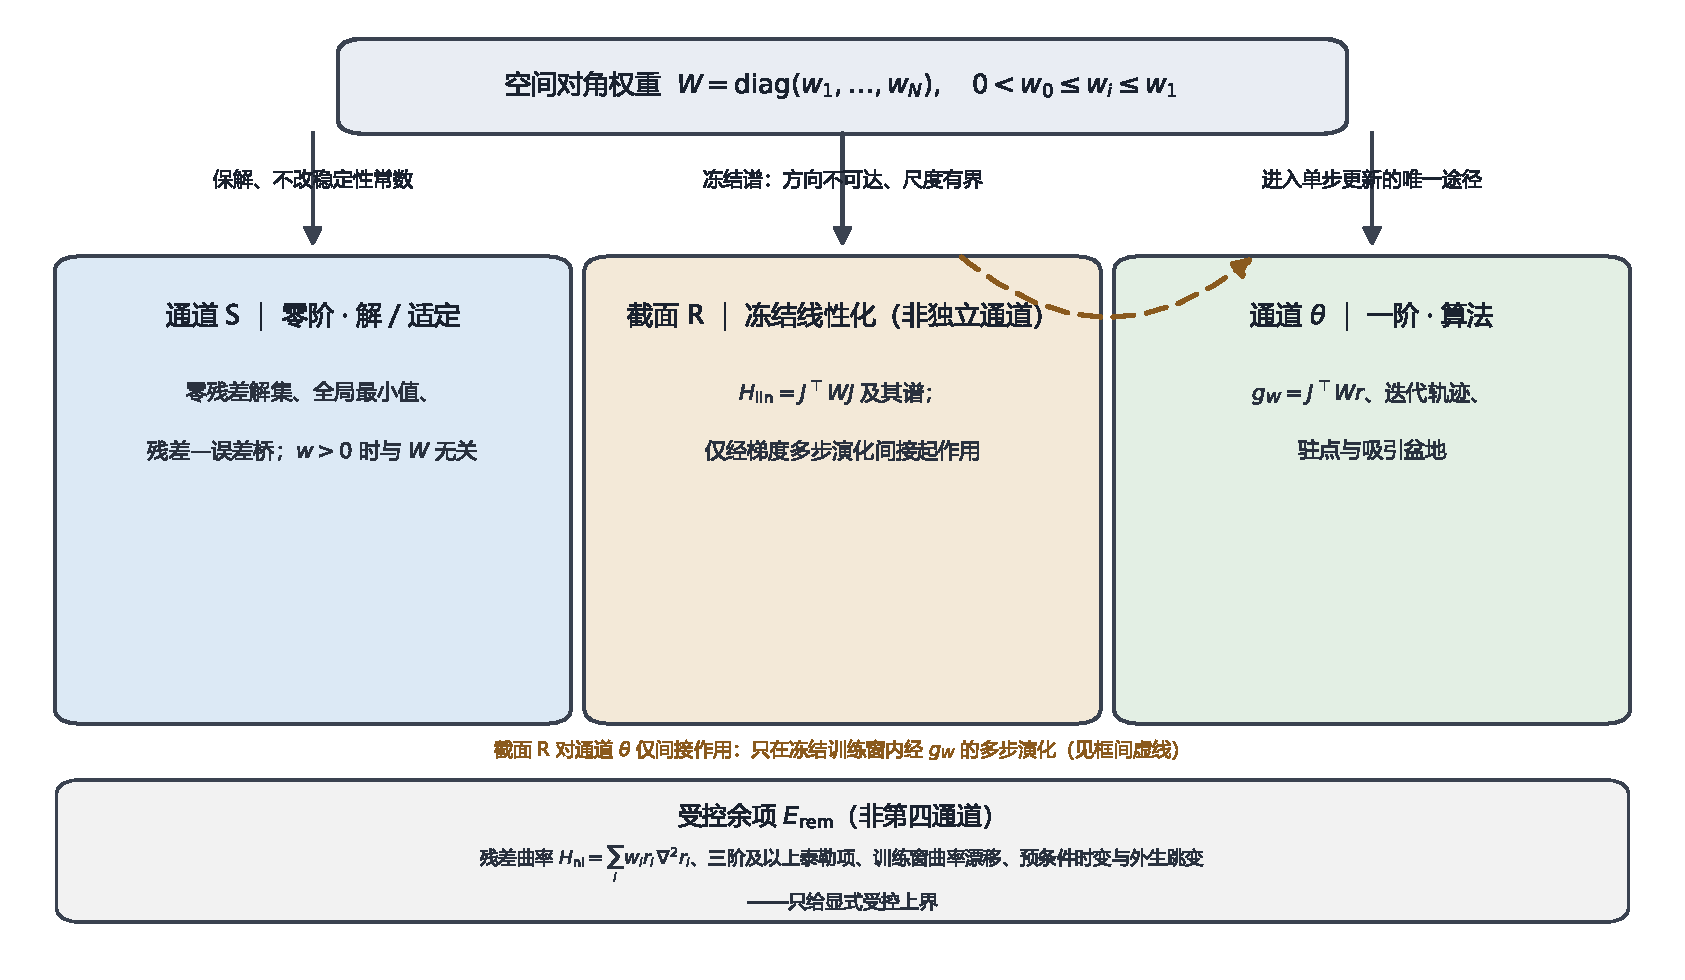
\includegraphics[width=0.99\linewidth]{fig_framework}
\caption{本文采用的分析层面区分：空间权重对零阶解、冻结线性化截面、一阶梯度场的作用分属三个不同层面，跨层结论不可互证；二阶层面仅在冻结训练窗内经加权梯度的多步演化间接作用于一阶层面（框间虚线），高阶与非线性项归为有界的受控余项。}\label{fig:box}
\end{figure}

\subsection{贡献}\label{sec:contrib}
凡属标准结果，本文引用并标注为"重述/应用"，只对真正新增的部分主张贡献。本文新增以下三项：

\begin{enumerate}[label=(\arabic*),leftmargin=2em,itemsep=2pt]
\item \emph{分析层面的区分与准入原则}：按 Taylor 展开阶数将空间加权作用区分为零阶（解/适定性）、一阶（梯度/优化动力学）、二阶（冻结线性化谱）三个层面，该区分仅用于组织分析、避免跨层结论互证；以"信息封闭、权重外生"两原则划定仅梯度算法类的准入边界，将自然梯度、K-FAC、可训练权、自适应采样等类外方法明确划在类外并逐一列举。
\item \emph{二阶层面的谱能力边界}：证明空间局部对角加权对冻结 Gram 的特征方向对齐整类不可达（相关矩阵不变量 $R(\tilde K_r)=R(K_r)$ 为核心观察），等相关阵上条件数已最优（定理~\ref{thm:equicorr}），其作用仅为原特征方向上的有界缩放（van der Sluis 带）；唯一能白化的非局部权 $\W\propto K_r^{-1}$ 稠密且 $O(N^3)$，在线训练不可行。实验 4.2 在真实 Burgers 冻结 Jacobian 上严格静态验证：无约束正对角权相对 Jacobi 均衡的改善比 $r=\kappa^*_{\rm diag}/\kappa(R)\in[.76,.87]$（$N\le512$，多起点下界，真实最优不低于此值）；注意 Jacobi 均衡 $w_i\propto(K_r)_{ii}^{-1/2}$ 本身已是空间局部对角权，实践者起点 $w\equiv1$ 的条件数 $\kappa(K_r)$ 远高于此（见实验 4.2 三元组（表~\ref{tab:f1d-triplet}））。实验 4.3 作为训练过程经验旁证：默认裁剪配置（clip=1）下减权族恶化 $1.7$--$4.9$ 倍（小粘性 $.001$/.005 档 $3.0$--$4.9$ 倍），裁剪关闭时区间更宽（$0.6$--$3.4$）且个别格出现改善。此处 $\kappa=\lambda_{\max}/|\lambda_{\min}|$ 采用代数极值口径、Lanczos 外缘估计，测完整 Hessian 而非冻结 $H_{\rm lin}$，仅作跨族排序用，不构成定理的严格动态验证。
\item \emph{受控证伪实验与能力边界刻画}：给出好盆地内增权的一阶方向判据，证明对齐角不能判别盆地好坏。通过 $n=80$ 配对 McNemar 检验（K=4 选优口径）拒绝"减权可提高盆地进入概率"假说（三族净救回均为负，uniform 命中率 $.613$ 反高于全部加权族，Holm 校正后仅 down\_lin 显著 $p=.006$；阈值 $\tau\in[.05,.08]$ 扰动下该结论稳健，$\tau<.05$ 因好盆地样本少而功效不足）。减权的均匀尺度分量被 Adam 逐维归一化吸收，其作用以梯度尺度调节为主（压低梯度峰值与硬裁剪率），实验 5.8 检测到残余空间再分配效应的边缘信号（down\_lin 推高有效 lr 上限一倍，精确双侧 $p=.0625$、渐近 $\approx.043$，方向一致但未达 $.05$ 显著），故不声称减权仅为纯尺度调节器；减权不放宽稳定步长、不提升盆地进入，终态收益仅在频谱失配时出现（见第~\ref{sec:crosseqn}~章）。全量 $n=11$ 实验表明固定增权强度的终态增益不显著，事后最优 $\beta^*$ 是描述性观察（单种子散布 $1$--$100$、对 $\nu$ 非单调），不构成可预训练部署的固定策略；固定高强度（$\beta=8$）的\emph{组中位}终态 $L_2$ 在窄宽度等配置下甚至反劣于 $\beta=1$（如宽度 $64$ 基准，组中位 $.0043\to.018$），说明增益对网络宽度敏感、固定强度并非普适增益。1584-run 退化扫描（实验 5.6）验证刚性端有增益、光滑端退化到误差地板。无真解部署时，残差/损失自评估类固定单投影标量受 Bayes 误差下界限制，四点 XOR 反例表明不可精确线性分离（最小错误 $1/4$）；携带空间对比度结构的量 $g_{et}$ 提供盆地判别可行性证据（proxy AUC $.971$，oracle AUC $.64$），是有噪声判别器，价值在于过滤明显坏盆地、减少无效精修。
\end{enumerate}

\subsection{组织结构与陈述约定}\label{sec:convention}
第~\ref{sec:related} 章梳理方法谱系并标明分界；第~\ref{sec:framework} 章给出记号、定义、准入原则与零阶基准；第~\ref{sec:R}--\ref{sec:crosseqn} 章依次给出二阶层面的谱能力边界、一阶层面的动力学边界、无真解盆地判别与跨方程验证；第~\ref{sec:conclusion} 章界定适用范围并总结。完整证明集中于附录~\ref{app:proof}，复现细节见附录~\ref{app:repro}，数值全量表见附录~\ref{app:data}--\ref{app:tables}，方法谱系表与实验图谱见附录~\ref{app:lineage}--\ref{app:atlas}。

全文采用三级陈述标记：\textbf{[确定]}表示结构性/代数恒真或标准定理的直接应用；\textbf{[以概率 $1-\delta$]}表示在显式随机假设下成立、$\delta$ 可由样本量控制；\textbf{[经验 $n=$]}表示受控实验结论，必同时报告样本量 $n$、离散度（中位与四分位距，或 Wilson 置信区间）与实际测试的参数网格。强断言词（必然、不可能、唯一、充要、保证）只允许出现在前两级、且所需假设与结论在同段一并给出；比喻性措辞不进入结论句。

\FloatBarrier

\section{相关工作}\label{sec:related}
本章按"解—梯度—截面—盆地"四个层面梳理文献，另设一节讨论零阶表示层面的干预；每节末以\emph{分界}标明本文与该路线的关系，完整谱系表见附录~\ref{app:lineage}。

\subsection{PINN 的严格数值分析与误差界}\label{sec:rel-error}
对 PINN 泛化误差的严格分析已形成体系：Mishra 与 Molinaro\cite{MishraMolinaro2020} 以前向稳定性结合训练误差与配点采样数给出泛化误差上界；De~Ryck 与 Mishra 给出 Kolmogorov 型 PDE 的误差估计，并对 PINN 的数值分析作系统综述\cite{DeRyckMishra2022,DeRyckMishra2024}；Shin 等证明线性二阶椭圆与抛物型 PDE 下 PINN 解在配点加密极限下的收敛性\cite{Shin2020}。这类工作回答"训练残差与采样数如何控制真误差"，对应本文零阶层面的残差—误差桥。\emph{分界}：本文的残差—误差桥是这些\emph{标准稳定性估计在空间加权范数下的重述}，不主张原创；新增之处仅在于明确稳定性常数与空间权重无关，并据此把"解的误差"与"优化轨迹的改善"严格分离。

\subsection{梯度病理、神经正切核与收敛率失配}\label{sec:rel-ntk}
Wang、Teng 与 Perdikaris\cite{WangTeng2020}系统刻画了 PINN 的梯度量级病理，并以学习率退火等手段缓解；Wang、Yu 与 Perdikaris\cite{Wang2020NTK}在 NTK 框架下证明，无限宽极限下训练由确定性核支配，\emph{不同损失项}的收敛率因核特征值不同而失配，并据此提出按特征值校准；该线性化（惰性训练）视角在非线性 regime 下的局限见\cite{Bonfanti2024}。\emph{分界}：上述 NTK 失配发生在\emph{不同损失分量之间}，而本文的特征方向边界（定理~\ref{thm:local-cap}）针对\emph{同一 PDE 残差内部}的空间对角权重 $\W$ 对冻结 Gram 特征方向的作用；二者层面不同，结论互补而不重叠。

\subsection{自适应配点与硬区加权/降权路线}\label{sec:rel-weight}
\emph{增权与自适应采样}方面，RAR/RAD 类方法按残差自适应补充配点（系统比较见\cite{Wu2022}，重要性采样见\cite{Nabian2021}，深度生成式自适应采样见\cite{TangDAS2023}），因果训练\cite{Wang2022causal}按时间因果结构加权；Self-Adaptive PINNs\cite{McClenny2020}以可训练软注意力逐点调整权重，因权重可训练、违反权重外生原则，属本文准入类外（第~\ref{sec:framework} 章）。\emph{降权}方面，Maddu 等\cite{Maddu2021}刻画多尺度失配这一失败模式并以逆 Dirichlet 权重缓解；Liu 等\cite{Liu2022down}在间断处\emph{减弱}网络表达、聚焦光滑区域；Wang 等\cite{LessEmphasis2022}提出少关注高损失区域的课程式策略。\emph{梯度冲突}方面，ConFIG\cite{ConFIG2025}在优化期对冲突梯度做冲突消除（以正交投影为手段）。近期，Si 与 Yan\cite{SiYan2025}从原对偶优化视角论证逐点权"原子化"、忽略空间相关，须改用空间相干的卷积（非局部）权才能稳定改善，这从方法侧独立印证本文定理~\ref{thm:local-cap}"局部权不足、有效白化须非局部"的结论。\emph{分界}：本文不提出又一种加权策略，而是给出"任意空间局部加权分别在解、梯度、截面三个层面能与不能做什么"的统一判定，并以配对实验厘清增权、减权各自的真实作用区间。

\subsection{条件数、最优权重与算子预条件}\label{sec:rel-precond}
在冻结、线性化视角下，"条件数决定一阶方法收敛率、并据此设计预条件器"已有系统工作。对线性、适定的 PDE，van~der~Meer、Oosterlee 与 Borovykh\cite{vanDerMeer2020}证明加权目标泛函的凸性并给出最优缩放，这是"加权不改变适定性、只改变条件数尺度"最直接的先例。de~Ryck 等\cite{deRyckOp2024}以算子预条件观点分析物理信息机器学习的训练：在冻结线性模型中把离散 Gram 与微分算子的 Hermitian 平方相联系，给出 $O(\kappa\log\varepsilon^{-1})$ 的梯度下降迭代复杂度，并以按算子谱缩放或稠密逆白化把条件数降至约 $1$；预条件 PINN（PCPINN\cite{PCPINN2024}）同样以条件数诊断训练，借鉴 PDE 离散算子的经典预条件（如不完全 LU 分解）改善求解（原文指出 ILU 不保证条件数严格下降，但经验上促进收敛）。在最优对角缩放一侧，给定矩阵的最优正对角预条件可经半定规划精确求解、并有近线性时间近似算法\cite{Qu2025ODP,Jambulapati2020,Gao2024SODP}；哪些矩阵类在对角缩放下已最优亦有经典刻画\cite{ForsytheStraus1955,Shapiro1982,LivneGolub2004}。面向多物理 PINN 的 Kronecker 块对角预条件\cite{KroneckerPINN2026}在跨方程块级施加预条件，而非场内逐点。\emph{分界}：上述预条件要么是稠密、非局部、依赖线性化点的算子级变换，要么改动优化器或网络架构；"非局部预条件能把条件数降到约 $1$"已由它们回答，本文不主张首创谱白化的可行性。本文新增的是其\emph{补集}：工程上最常用的\emph{空间局部、逐点对角}权重这一受限类为何做不到（定理~\ref{thm:local-cap} 的相关矩阵不变量与 van~der~Sluis 界）。此外，本文零阶层面的加权范数双向夹逼可视为\cite{vanDerMeer2020}凸性结论在非线性局部情形的延伸；二阶层面的特征值尺度界则进一步说明，即便在线性情形，空间\emph{异速}（非乘性常数）加权对条件数的净效果仍是双向不定的。与最优对角预条件文献的分工：后者对\emph{给定}矩阵求最优对角缩放（计算问题），本文刻画空间局部对角权\emph{整类}在特征方向上的不可达性（能力边界），并以实验 4.2 量出最优缩放离白化的实际距离。

\subsection{盆地可达性、课程与同伦}\label{sec:rel-curriculum}
Bengio 等\cite{Bengio2009}建立课程学习即连续化（continuation）、影响局部极小质量的一般观点；连续化方法的优化理论可追溯至 Gaussian 同伦与毕业优化\cite{Mobahi2015,Hazan2016}，梯度方法在孤立鞍点条件下几乎必然收敛于极小点\cite{Lee2016}。Krishnapriyan 等\cite{Krishnapriyan2021}系统刻画 PINN 的失败模式，并以 curriculum/sequential 正则显著降低误差；损失景观视角下 PINN 训练困难的系统分析见\cite{Rathore2024}；另有工作指出失效模式的相当部分源于单精度浮点误差而非损失景观本身，改用 FP64 即可消除\cite{FP64Xu2025}——这与本文视角互补：精度决定残差能否被压下去，盆地结构决定压下去的是否为真解。在伪解一侧，Rohrhofer 等\cite{Rohrhofer2022}指出动力系统 PINN 会在平凡固定点附近最小化残差、让非物理解主导吸引域；Wang 等\cite{WangPseudo2026}针对"小残差但物理解错误"的伪解，用 pseudo-time 步进与重采样加以揭示和规避；以重采样缓解传播失败的 R3 采样亦属此脉络\cite{Daw2022Evo}。PINN 存在伪解吸引域、且 continuation/重采样/缩域有助于规避，这一现象本身归上述文献。与本文第~\ref{sec:methods} 章最接近的是 Musah\cite{Musah2026}：它在多场约束系统中独立、系统地报告了单一聚合残差会以高频率选择更差的解，并提出 lexicographic 可接受性门控。\emph{分界}：本文让渡"单一标量残差不能可靠选解"这一一般观察，新增之处是空间加权盆地判别语境下的四点严格反例与不依赖残差自评估的结构量。

\subsection{零阶表示层面干预：硬约束 ansatz、坐标变换与初始化}\label{sec:rel-repr}
另有一类工作不改动损失权重，而直接改动网络的零阶表示。其一是\emph{硬约束 trial 函数/输出变换}：以距离函数与 R--函数构造湮灭因子、在输出端逐点精确满足 Dirichlet/Neumann/Robin 条件\cite{Sukumar2022distance}，或把线性 PDE 编码为输出层超平面而使方程被逐点满足\cite{Leng2022hyperplane}；其二是\emph{输入/坐标变换}：以变量缩放或坐标映射（平移、缩放）缓解薄层与刚性，Guan 与 Elman\cite{GuanElman2024}并以 NTK 解析地说明输入变换如何改变有效核；其三是\emph{初始化与表示带宽}：随机初始化与深集成被用于发现 PDE 的多个解\cite{Zou2025ensemble}。\emph{分界}：上述构造分别改变前向 ansatz 的边界提升、湮灭因子、坐标映射，或初值/频率，即都作用在零阶表示层面；它们是各自孤立的单层干预，既未给出"零阶表示—二阶谱—一阶优化"的层间不可替代分类，也未区分"可表达"与"可到达"。

\FloatBarrier

\section{记号、定义与零阶基准}\label{sec:framework}

\subsection{记号与加权训练目标}\label{sec:notation}
设网络 $u(x;\theta)$（$\theta\in\R^p$）逼近 PDE $\mathcal N[u]=0$ 的解 $u^*$；本文全部实验中初边值条件由硬约束 ansatz 精确满足（属零阶表示层面干预，参见第~\ref{sec:rel-repr} 节），残差向量只含内部配点。在配点 $\{x_i\}_{i=1}^{N}$ 处定义 $r(\theta)=(r_1,\dots,r_N)^\top$，$r_i=\mathcal N[u](x_i;\theta)$，雅可比 $J(\theta)=\partial_\theta r\in\R^{N\times p}$。\emph{空间对角权重}为 $\W=\diag(w_1,\dots,w_N)$，$w_i\ge0$ 由外生规则给出：逐点自变量为残差对比度 $t_i$（式~\eqref{eq:t-contrast}），全局强度 $\beta$ 为外生超参；权重在快照间冻结、不与 $\theta$ 联合训练（对应定义~\ref{def:admit} 原则~II 的冻结分支；盆地进入实验的在线重算口径属探测性设计，协议声明见第~\ref{sec:theta-exp} 节，冻结实现细节见附录~\ref{app:repro}）。加权训练目标取经验平均（与 PINN 原始 MSE 及最优加权损失的标准口径一致\cite{Raissi2019,vanDerMeer2020}）：
\begin{equation}\label{eq:lw}
L_{\W}(\theta)=\tfrac{1}{2N}\sum_{i=1}^{N}w_i r_i^2=\tfrac{1}{2N} r(\theta)^\top \W r(\theta).
\end{equation}
全文设 $\W$ 属于正定对角锥 $\mathcal W_+=\{\W:0<w_0\le w_i\le w_1<\infty\}$，记权重条件数 $\kappa_{\W}=w_1/w_0$；本文部署的权重族均严格满足 $w_i>0$（见第~\ref{sec:family} 节）。经验平均口径下一阶梯度与 Hessian 为
\begin{equation}\label{eq:h-split}
g_{\W}:=\tfrac1N J^\top\W r,\qquad
H_{\W}:=\nabla_\theta g_{\W}
=\underbrace{\tfrac1N J^\top\W J}_{H_{\rm lin}}
+\underbrace{\tfrac1N\sum_{i=1}^{N}w_i r_i\,\nabla_\theta^2 r_i}_{H_{\rm nl}} ,
\end{equation}
其中 $H_{\rm lin}=\tfrac1N J^\top\W J$ 为 Gauss--Newton 项（只含残差的一阶导、与残差幅值无关），$H_{\rm nl}$ 为残差曲率项（关于残差线性、随残差趋零而消失）；此即标准 Gauss--Newton 分解。\emph{公共因子约定}：$1/N$ 是与方向无关的公共正标量，不改变特征向量、惯性指数、条件数与零空间；故自截面谱刻画起，凡只涉及方向、谱结构与惯性之处，均把该公共因子吸收进记号、仍写 $J^\top\W J$。注意 $J$、$J^\top J$ 与 Fisher 信息阵 $F(\theta)=J^\top J$（等权情形）均\emph{不含}空间权重 $\W$。

\noindent\emph{全文范数约定。}向量欧氏范数 $\norm v=(v^\top v)^{1/2}$；预条件 $P_t\succ0$ 下的加权范数 $\norm v_{P_t}^2=v^\top P_t v$（梯度下降 $P_t=I$ 时即欧氏范数）；函数空间 $\norm f_{L^2}=(\int|f|^2)^{1/2}$、加权 $\norm f_{L^2(w)}=(\int w|f|^2)^{1/2}$，其离散对应为 $\ell^2$ 范数与 $\norm r_\infty=\max_i|r_i|$；矩阵默认谱范数 $\norm A_2$，用到 Frobenius 范数 $\norm A_F$ 处显式标出。\emph{白化约定（贯穿优化动力学分析）}：对正定预条件 $P_t\succ0$，记白化量 $\wt g:=P_t^{1/2}g$、$\wt H_{\rm lin}:=P_t^{1/2}H_{\rm lin}P_t^{1/2}$、$\wt H_{\rm nl}:=P_t^{1/2}H_{\rm nl}P_t^{1/2}$；白化后一律取欧氏范数，条件数因子只在结论转回原始空间时出现一次（$P_t=I$ 时全部退化为恒等）。

\subsection{权重族与有理增权族}\label{sec:family}
以逐点\emph{残差对比度}
\begin{equation}\label{eq:t-contrast}
t_i=\frac{|r_i|}{\operatorname{median}|r|+\epsilon}\ge0,\qquad \epsilon>0
\end{equation}
为自变量；$\operatorname{median}|r|$ 取全部 $N$ 个配点残差幅值的中位数，$\epsilon=10^{-12}$ 仅防除零、不参与量级（实现口径见附录~\ref{app:repro}）。本文比较六族权重：三族增权（rational、linear、band）、两族减权（down\_lin、down\_inv）与等权 uniform。主族为\emph{有理增权族}。记 $q=t/(1+t)\in[0,1)$、$\bar q(t)=\min\{t,1\}$（截断到 $[0,1]$）、$\mathbf 1\{\cdot\}$ 为示性函数，代码实现与全部实验统一采用下列显式形式：
\begin{equation}\label{eq:families}
\begin{aligned}
&\text{rational:}\ \ w=1+(\beta-1)q=\tfrac{1+\beta t}{1+t},
&\text{linear:}\ \ w&=1+(\beta-1)\bar q(t),\\
&\text{band:}\ \ w=1+(\beta-1)\mathbf 1\{q>\tfrac12\},
&\text{uniform:}\ \ w&\equiv1,\\
&\text{down\_lin:}\ \ w=1-(1-\beta^{-1})q,
&\text{down\_inv:}\ \ w&=\tfrac{1}{1+(\beta-1)q}=\tfrac{1+t}{1+\beta t}.
\end{aligned}
\end{equation}
三族增权均夹在 $[1,\beta]$、两族减权均夹在 $[\beta^{-1},1]$（端点为 $t\to\infty$ 极限，或由截断/示性函数达到）；理论分析以 rational 为主族，其余五族用于受控对照，论文与代码的代数式一律以式~\eqref{eq:families} 为准。

\begin{definition}[有理增权族与 $\phi$]\label{def:w}
对对比度 $t\ge0$ 与强度 $\beta\ge1$，有理增权权函数与\emph{梯度分量对比度}为
\begin{equation}\label{eq:rational}
w(t;\beta)=\frac{1+\beta t}{1+t},\qquad \phi(t;\beta)=t\,w(t;\beta)=\frac{1+\beta t}{1+t}\,t .
\end{equation}
其中 $\phi=tw$ 是加权梯度分量 $w_i r_i J_i$ 的对比度幅值（属一阶层面）；机制~A 中增权对梯度能量的再分配经 $\partial_\beta w$ 实现，与 $\phi'$ 无关（见第~\ref{sec:theta-mechA} 节）。$\phi=tw$ 须与\emph{损失层幅值} $t\sqrt w$（单点损失密度 $\sqrt w\,|r|$ 的对比度，属零阶层面、与残差—误差桥双向界同口径）区分，二者差一个 $\sqrt w$ 因子、不可混用。
\end{definition}

有理增权满足 $w(0)=1$、$w(\infty)=\beta$、$w'(t)=(\beta-1)/(1+t)^2\ge0$，故 $1\le w\le\beta$、关于 $t$ 单调有界饱和。线性减权为 $w^{dn}_{lin}=1-(1-1/\beta)q\in[1/\beta,1]$（与式~\eqref{eq:families} 的代码实现一致），逆式减权为 $w^{dn}_{inv}(t)=(1+t)/(1+\beta t)\in[1/\beta,1]$，是增权有理形在分子/分母互换意义下的对偶，二者端点同为 $\{1,1/\beta\}$、均随 $t$ 递减（与增权族相反）。等权族恒为 $1$。

主族的单点加权损失密度为 $\Psi_2(t)=w(t)\,t^2$（对 $t$ 取加权 $L^2$、等效权重恰为 $w$），全文统一采用该口径。沿单一残差径向 $\Psi_2''(t)=2(1+3\beta t+3\beta t^2+\beta t^3)/(1+t)^3>0$，故 $\Psi_2$ 在整个 $\beta\ge1,t\ge0$ 区域严格\emph{一维径向凸}。该凸性仅是残差幅值一维径向的设计自检性质，不蕴含参数空间 $\theta$ 中优化景观的任何（局部或全局）凸性。

\subsection{仅梯度算法类的准入：信息集与两原则}\label{sec:admit}
本文的理论分析限定在\emph{仅梯度算法类}（gradient-only class），即单步参数更新只读取当前点的加权梯度 $g_\W$（及由梯度构造的辅助态）、不直接读取 Hessian、Jacobian 谱或标量损失景观的算法。典型代表包括梯度下降（GD）、带动量的 GD、Adam 及其变体；L-BFGS 等拟牛顿法若使用基于 $|g_\W|$ 的步长规则可归入此类，但若线搜直接读取 $L_\W$ 则落在类外（见定义~\ref{def:admit} 的类外方法列表）。

\begin{definition}[信息集与两原则]\label{def:admit}
设单步更新为 $\theta_{k+1}=\theta_k-\eta_k A_k g_\W(\theta_k)$，其中 $A_k$ 为预条件矩阵。称该算法属于仅梯度类，当且仅当以下两条原则成立：
\begin{enumerate}[label=\textup{(P\arabic*)},leftmargin=2em]
\item \emph{信息封闭}：$A_k$ 与步长 $\eta_k$ 只依赖于过去梯度序列 $\{g_\W(\theta_j)\}_{j\le k}$（及由梯度构造的辅助态，如动量、Adam 二阶矩），不直接读取标量损失值 $L_\W$、$J(\theta_k)$、$H_{\rm lin}(\theta_k)$ 或其谱。
\item \emph{权重外生}：空间权重 $\W$ 在训练窗内冻结或由外生缓变过程给定，不依赖于当前参数 $\theta_k$ 的可微函数；即 $\nabla_{\theta_k}\W=0$（冻结）或 $\|\nabla_{\theta_k}\W\|$ 被显式小量控制（缓变；量化口径见假设~\ref{ass:ctrl} 的 (Q4) 与注记~\ref{rem:adam-drift}）。
\end{enumerate}
\end{definition}

两原则的意义在于：在收紧的 (P1)(P2) 下，$\W$ 进入单步更新的唯一微分途径是加权梯度 $g_\W=J^\top\W r$，截面 $H_{\rm lin}=J^\top\W J$ 不被单步直接读取。这是全文层面区分的算法前提。若算法直接读取 $L_\W$（如标准 Armijo 线搜），则 $L_\W$ 本身携带 $\W$，"唯一途径"不再成立，这类算法落在类外。

\emph{类外方法}（不满足 (P1) 或 (P2)）包括：自然梯度（$A=G^{-1}$ 直接读取 Fisher 信息阵，违反 P1）、K-FAC（块近似 Fisher，违反 P1）、\emph{基于标量损失的线搜/步长调度}（如标准 Armijo 回溯，违反 P1）、可训练权重（$\W=\W(\theta)$ 可微，违反 P2，如 Self-Adaptive PINNs\cite{McClenny2020}）、自适应采样 RAR/RAD（改变配点集而非固定权重，属另一类干预）、稠密算子预条件（直接读取微分算子谱，违反 P1）。这些方法不在本文理论覆盖范围内，但其作用层面可由上述分层定位：自然梯度/预条件作用在二阶层面（试图白化 $H_{\rm lin}$），可训练权重作用在一阶与二阶层面的接口（$\W$ 随 $\theta$ 变化引入额外梯度项），自适应采样改变配点测度（属零阶对象变化）。

\subsection{零阶层面：保解不变与残差—误差桥}\label{sec:Schan}
在固定权重族（第~\ref{sec:family}~节）与算法准入类（第~\ref{sec:admit}~节）之后，本节固定不依赖这两者的零阶对象：零残差解集、全局最小值与残差到误差的稳定性桥。它们是分层框架的公共基准——后续二阶（第~\ref{sec:R}~章）与一阶（第~\ref{sec:theta}~章）的分析都在此基准上叠加权重与算法效应；零阶对象本身不随 $\W$ 改变、结论短小，故不单列一章。以下结果是标准稳定性估计在空间加权范数下的重述，本文不主张原创。

\begin{proposition}[零解集不变]\label{prop:zero}
设 $\W=\diag(w_i)$ 满足 $w_i>0$ 对所有 $i$ 成立。则加权损失 $L_\W(\theta)=\tfrac12 r(\theta)^\top\W r(\theta)$ 与等权损失 $L_I(\theta)=\tfrac12\|r(\theta)\|^2$ 的零残差解集完全相同；在零残差可达（适定且表示充分）时，两者的全局最小点集均等于 $\{\theta:r(\theta)=0\}$。
\end{proposition}
证明是逐元代数验证，见附录~\ref{app:proof}。

命题~\ref{prop:zero} 的意义是：空间加权不改变"哪些参数点是方程的精确解"，也不改变全局最小值的位置（在残差可零的适定问题中）。因此，声称"加权改善了优化"不能以"零解集不变"为依据——零阶对象与一阶动力学是两个独立层面。

\begin{assumption}[适定性输入，引用性]\label{ass:wellposed}
设 PDE 算子 $\mathcal N$ 在解 $u^*$ 附近的线性化有界可逆，存在稳定性常数 $C_{\rm stab}>0$ 使得对足够小的残差 $r=\mathcal N[u_\theta]$，有
\begin{equation}\label{eq:bridge}
\|u_\theta-u^*\|_{L^2}\le C_{\rm stab}\,\|r\|_{L^2},
\end{equation}
其中 $\|r\|_{L^2}^2=\int_\Omega |\mathcal N[u_\theta](x)|^2 dx$。该类估计是 PINN 误差分析的\emph{标准输入}而非本文结果：一般情形见\cite{MishraMolinaro2020,DeRyckMishra2022}，线性二阶椭圆/抛物方程有严格证明见\cite{Shin2020}，粘性 Burgers 方程（本文主 testbed）的 DNN 显式误差估计见\cite{Akram2025}。对 Burgers 行波内部层的干净范数估计本文不断言已证，只取形式量级（口径见附录~\ref{app:proof}）。
\end{assumption}

\begin{proposition}[残差—误差桥的加权版]\label{prop:bridge}
在假设~\ref{ass:wellposed} 下，对加权范数 $\|r\|_{L^2(w)}^2=\int_\Omega w(x)|\mathcal N[u_\theta](x)|^2 dx$，当 $w_0\le w(x)\le w_1$ 时，有双向夹逼
\begin{equation}\label{eq:bridge-weighted}
w_0^{1/2}\|r\|_{L^2}\le \|r\|_{L^2(w)}\le w_1^{1/2}\|r\|_{L^2}.
\end{equation}
因此稳定性常数 $C_{\rm stab}$ 与空间权重无关，加权只改变残差范数的标度（最坏情形引入 $w_0^{-1/2}$ 标度因子）、不改变适定性。
\end{proposition}
证明是逐元代数验证，见附录~\ref{app:proof}。

命题~\ref{prop:bridge} 的意义是：空间加权不改变 PDE 的适定性，只改变残差范数的标度。减权（$w_0<1$）会放大加权范数下的稳定性常数（最坏情形 $\sqrt{\beta}$ 倍），但这是标度效应、不是适定性变化。增权（$w_1>1$）不放宽原始 $L^2$ 稳定性常数。这一区分是后续"减权代价"分析的基准。（记号说明：附录证明中的 $C_{pde}$、$C_{loc}$ 与本节 $C_{\rm stab}$ 口径相同，均指（线性化）算子逆的范数界；离散配点与连续积分之间的求积/采样误差计入引理~\ref{lem:3comp} 的 $\varepsilon_{quad}$。）

\begin{corollary}[范数界与减权界]\label{cor:normbd}
增权归一化（$w_0=1$、$w_1=\beta$）下 $\|r\|_{L^2}\le\|r\|_{L^2(w)}\le\sqrt\beta\,\|r\|_{L^2}$，原始 $L^2$ 稳定性常数不变；减权（$w_0=1/\beta$、$w_1=1$）下 $\beta^{-1/2}\|r\|_{L^2}\le\|r\|_{L^2(w)}\le\|r\|_{L^2}$，且 $\|u_\theta-u^*\|_{L^2}\le C_{\rm stab}\sqrt\beta\,\|r\|_{L^2(w)}$：减权在加权范数下最坏放大稳定性常数 $\sqrt\beta$ 倍。
\end{corollary}
证明是逐元代数代入，见附录~\ref{app:proof}。

\begin{corollary}[非线性余项界]\label{cor:nonlin}
设 $-r_\theta=\Lop_*e+R_2$（$\Lop_*$ 为假设~\ref{ass:wellposed} 的线性化算子，$e=u_\theta-u^*$），非线性余项满足 $\|R_2\|\le L_N\|e\|_{L^2}^2$。则对满足 $2C_{\rm stab}L_N\rho_{\rm bas}\le\tfrac12$ 的误差半径 $\rho_{\rm bas}$，在 $\|e\|_{L^2}\le\rho_{\rm bas}$ 内有 $\|e\|_{L^2}\le 2C_{\rm stab}w_0^{-1/2}\|r_\theta\|_{L^2(w)}$。对 Burgers 行波 $L_N=1/(2\nu)$，形式标度 $\rho_{\rm bas}(\nu)=O(\nu^2)$ 及其适用限制见附录~\ref{app:proof}。
\end{corollary}
证明及 $C_{loc},\rho_{\rm bas}(\nu),R_r(\nu)$ 的显式估计见附录~\ref{app:proof}。

\begin{lemma}[三分量分解]\label{lem:3comp}
以 $u_m^*$ 记网络类最优表示、$u_{\mathcal S}$ 记采样与求积对应的中间量，则总误差分解为 $\|u^*-u_{\theta_T}\|\le\varepsilon_{app}+\varepsilon_{gen}+\varepsilon_{quad}+\varepsilon_{opt}$：表示误差 $\varepsilon_{app}$ 只由表示容量决定、与 $w$ 无关；泛化/求积项 $\varepsilon_{gen}+\varepsilon_{quad}$ 经命题~\ref{prop:bridge} 只获 $O(\sqrt\beta)$ 常数依赖；仅优化项 $\varepsilon_{opt}$ 与加权动力学强相关。
\end{lemma}
证明见附录~\ref{app:proof}。

\FloatBarrier

\section{二阶层面：局部对角权的谱能力边界}\label{sec:R}

本章研究冻结线性化截面 $H_{\rm lin}=J^\top\W J$ 的谱随空间对角权重 $\W$ 的变化。核心问题是：\emph{仅靠给不同空间配点赋不同权重，能否把这张二次型变得不那么病态}。结论是：局部对角权能改变特征值尺度，却改变不了配点间的相关结构（特征方向），而后者恰是刚性问题病态的根源。本章先给出冻结线性化的分析框架，再证明核心定理，最后以真实 Burgers Jacobian 的静态 N 扫描与训练过程 Hessian 条件数的动态记录双重验证。

\subsection{全局假设与冻结线性化框架}\label{sec:R-frame}

下列三组假设贯穿二阶与一阶层面的理论分析，显式标注其性质。

\begin{assumption}[G-A 可表示性，静态]\label{ass:GA}
给定 Fourier 带宽 $\sigma$ 覆盖激波尺度 $O(\nu)$，网络类中\emph{存在}参数 $\theta_m^*$ 使 $\|u^*-u(\cdot;\theta_m^*)\|\le\varepsilon_{app}$（三分量分解的表示分量，引理~\ref{lem:3comp}）。该\emph{存在性}是神经网络通用逼近与 PINN 一致性/泛化误差估计的标准结论\cite{Shin2020,MishraMolinaro2020,DeRyckMishra2024}，\emph{不依赖具体方程}；本文只断言存在、不断言训练能找到（可达性属 G-B）。\emph{与方程相关的只是标度常数}：对基准真解 $u^*=-\tanh(x/(2\nu))$，其 $k$ 阶导含因子 $\nu^{-k}$，故达到固定 $\varepsilon_{app}$ 所需宽度与带宽随 $\nu\downarrow$ 升高，此为方程固有难度、与权重无关。
\end{assumption}

\begin{assumption}[G-B 盆地可达，Phase~0，概率性]\label{ass:GB}
以 $p_{entry}=\Pr_{\theta_0,\mathcal S}[\theta(T_0)\in B(u^*);\mathcal C_\sigma,\mathcal O]$ 表示在表示课程 $\mathcal C_\sigma$ 与优化器 $\mathcal O$ 下于 $T_0$ 进入真解盆地的概率。不假设 $p_{entry}=1$，只研究其对 $\sigma$、宽度、初始化与多起点数 $K$ 的依赖。
\end{assumption}

\begin{assumption}[G-C 盆地内局部良性，Phase~1，弱化版]\label{ass:GC}
进入 $B(u^*)$ 且权重冻结或\emph{外生缓变}时（本文结论针对冻结 $\W$，或由训练时间表/未加权量触发的外生缓变 $\W$；在线自适应或可训练 $\W(\theta)$ 违反原则~II、超出仅梯度算法类，列入未来工作）：
\par(i)~\emph{有效子空间非退化}：梯度 Krylov 子空间 $V_g=\spanop\{g,H_{\W}g,\ldots\}$ 上最小 Ritz 值 $\lambda_{\min}(V_g^\top H_{\W}V_g)\ge\lambda_*(\nu)>0$（不要求全空间 Hessian 正定）；
\par(ii)~\emph{训练窗内有界漂移}：存在 $\varepsilon_{NTK}<1$ 使 $\sup_{0\le t\le T_1}\|K_r(t)-K_r(0)\|/\|K_r(0)\|\le\varepsilon_{NTK}$（有限宽训练窗，不要求 $m\to\infty$ 的渐近）；
\par(iii)~\emph{{\L}ojasiewicz 局部良性}：在误差半径 $\rho_{\rm bas}(\nu)$（存在性与形式标度见推论~\ref{cor:nonlin}）内 $\|\nabla L_{\W}\|\ge c_L|L_{\W}-L_{\W}^\star|^\vartheta$，$\vartheta\in[1/2,1)$。对实解析激活（如 sin、tanh）的 Fourier 特征网络，残差是参数的实解析函数、由解析性\emph{推出}局部 {\L}ojasiewicz 不等式，故 (iii) 更接近推论而非额外假设。
\emph{G-C 自始至终不要求、也不蕴含空间加权能实现谱白化}（谱白化指经加权使冻结 Gram 的条件数化为 $1$、即 $\W\propto K_r^{-1}$；它对空间局部加权整类不可达，见定理~\ref{thm:local-cap}）。
\end{assumption}

设网络残差在训练窗内足够光滑（$r\in C^{2,1}$，即二阶导 Lipschitz，光滑激活下即满足）。一般一阶算法的单步更新为
\begin{equation}\label{eq:onestep}
\theta_{k+1}=\theta_k-\eta P_t g_k,\qquad P_t\succ0,
\end{equation}
其中 $P_t$ 由 $k$ 步信息集构造：梯度下降 $P_t=I$、Adam $P_t=D_t^{-1}$（$D_t=\diag(\hat v_t)+\epsilon I$ 为偏差校正二阶矩对角阵）、固定步长 L-BFGS $P_t=B_k^{-1}$。式~\eqref{eq:onestep} 对带动量算法取忽略动量方向的理想化（即把 Adam 视为对角预条件梯度步）；该理想化不改变结论级别——Adam 下引理~\ref{lem:linrec} 的定量窗内界本就退化为非扩张上界（注记~\ref{rem:adam-drift}）。对 $P_t$ 取唯一对称正定平方根 $P_t^{1/2}$，定义\emph{白化量}
\begin{align}
\wt g:=P_t^{1/2}g,\quad \wt H_{\rm lin}:=P_t^{1/2}H_{\rm lin}P_t^{1/2},\quad
\wt H_{\rm nl}:=P_t^{1/2}H_{\rm nl}P_t^{1/2},\quad \wt H_{\W}:=\wt H_{\rm lin}+\wt H_{\rm nl}.\label{eq:white}
\end{align}
齐次算子 $M=I-\eta H_{\rm lin}P_t$ 的白化相似形为 $\wt M=I-\eta\wt H_{\rm lin}$，因 $\wt H_{\rm lin}$ 对称半正定，$\wt M$ 是\emph{对称}矩阵，可直接使用欧氏谱定理。由\emph{线性化}主部生成的 Krylov 子空间称为线性化行走子空间 $\wt V_g^{lin}:=\mathcal K(\wt H_{\rm lin},\wt g_k)=\spanop\{\wt g_k,\wt H_{\rm lin}\wt g_k,\ldots\}$；取其欧氏标准正交基 $Q$，定义白化最小/最大 Ritz 值 $\lambda_V^{(P)}:=\lambda_{\min}(Q^\top\wt H_{\rm lin}Q)$、$\widehat\lambda_V^{(P)}:=\lambda_{\max}(Q^\top\wt H_{\rm lin}Q)$。

\begin{corollary}[白化非退化：加权不改变零空间]\label{cor:ker}
对任意 $\W\succ0$ 与正定 $P_t$，有：(i)~$\ker\wt H_{\rm lin}=P_t^{-1/2}\ker J$，右端不含 $\W$，空间加权无法创造或消灭零空间方向；(ii)~Loewner 单调：$\W_1\preceq\W_2\Rightarrow Q^\top\wt H_{\rm lin}^{(1)}Q\preceq Q^\top\wt H_{\rm lin}^{(2)}Q$（对任一固定欧氏标准正交基 $Q$ 成立）；(iii)~线性化行走子空间非退化恒成立：$\lambda_V^{(P)}>0$ 是代数推论，只需 $g\in\operatorname{range}J^\top$、$\W\succ0$、$P_t\succ0$ 与当前非停滞，\emph{不需要}受控条件。
\end{corollary}
证明是逐元代数验证，见附录~\ref{app:proof}。

\noindent\emph{计算直观。}空间加权消不去白化 Jacobian 的零空间：若某行走方向本就落在 $\ker J$（网络表达不到的模态），再怎么调权也不会产生有限收缩率，只能改 $J$ 本身（加宽、加带宽、换表示、多起点）。

\subsection{线性化递推与窗内收缩}\label{sec:R-linrec}

\begin{assumption}[线性化窗口的受控条件]\label{ass:ctrl}
在训练窗 $T_w$ 内同时满足：(P)~预条件正定、窗内谱有界且平方根\emph{相对}缓变（$0<p_{\min}I\preceq P_t\preceq p_{\max}I$，$\sum_{j<n}\|P_{k+j+1}^{1/2}-P_{k+j}^{1/2}\|/\|P_k^{1/2}\|\le\delta_P$；相应绝对漂移为 $\|P_k^{1/2}\|\,\delta_P$，该因子在引理界常数 $C_{\rm drift}$ 中显式携带，因 $\|P_k^{1/2}\|\le\sqrt{p_{\max}}$ 故为常数、不改变渐近阶）；(Q0)~窗内白化梯度有界 $\sup_k\|\wt g_k\|\le\bar g$，$\bar g$ 不依赖步长 $\eta$；(Q1)~局部残差幅值 $\bar r:=\|r\|_\infty$；(Q2)~曲率与三阶界 $\sup_i\|\nabla_\theta^2r_i\|\le L_r$，$g\in C^{1,1}$；(Q3)~小步长与配对条件 $\eta\|\wt H_{\rm lin}\|\le c_0<1$，$\eta L_3\|P_tg\|\le c_1\lambda_V^{(P)}$（$c_1\ll1$）；(Q4)~短窗缓变：窗内 $H_{\W}$ 与 $\W$ 冻结或外生缓变，预条件器满足 (P) 的缓变条件（不要求 $P_t$ 严格冻结），窗长 $n\le\varepsilon_H\|H_{\W}\|/(\eta L_3a_P\bar g)$。
\end{assumption}

\begin{lemma}[线性化递推、余项界与窗内多步收缩（白化空间陈述）]\label{lem:linrec}
在式~\eqref{eq:onestep}--\eqref{eq:white} 的白化框架、假设~\ref{ass:ctrl} 与推论~\ref{cor:ker} 的非退化下，有：
\begin{enumerate}[label=(\roman*),leftmargin=2.4em,itemsep=3pt]
\item \textbf{白化线性化恒等式}：$\wt g_{k+1}=(I-\eta\wt H_{\rm lin})\wt g_k+\wt\Erem_k+\wt\delta_k$，其中 $\wt\Erem_k=-\eta\wt H_{\rm nl}\wt g_k+\wt\rho_k$，$\|\wt\rho_k\|\le\tfrac{\eta^2}{2}L_3a_P^3\|\wt g_k\|^2$，$\|\wt\delta_k\|\le p_{\min}^{-1/2}(1+\eta\|\wt H_{\W}\|)\|P_{k+1}^{1/2}-P_k^{1/2}\|\,\|\wt g_k\|$；
\item \textbf{残差曲率受控}：$\|H_{\rm nl}\|\le w_1L_r\bar r$（此处取 $\infty$ 口径 $\bar r=\|r\|_\infty$；若取 $\ell_2$ 口径则上界为 $w_1L_r\,\mathrm{RMS}(r)=w_1L_r\|r\|_2/\sqrt N$，含 $1/\sqrt N$ 因子，两口径等价），固定 $N$ 而 $\bar r\to0$ 时 $H_{\rm nl}\to0$；
\item \textbf{单步相对界}：白化单步主驱动力满足 Ritz 下界 $\wt d_k:=\wt g_k^\top\wt H_{\rm lin}\wt g_k/\|\wt g_k\|\ge\lambda_V^{(P)}\|\wt g_k\|$，且 $\|\wt\Erem_k\|/(\eta\wt d_k)\le a_P^2w_1L_r\bar r/\lambda_V^{(P)}+\eta a_P^3L_3\bar g/(2\lambda_V^{(P)})=:\wt\varepsilon_{\rm lin}\xrightarrow[\bar r\to0,\eta\to0]{}0$；
\item \textbf{时变预条件器下的窗内界与长期行为}：定义有效平均收缩率 $\bar\rho:=\exp\!\bigl(\tfrac1n\sum_{j=0}^{n-1}\log\|\wt M_{k+j}\|_{V_g}\bigr)$，其中 $\|\wt M_{k+j}\|_{V_g}\le 1-\eta\lambda_V^{(P)}+O(\|P_k^{1/2}\|\delta_P/n)$（$\delta_P$ 为 (P) 中预条件器平方根的窗内\emph{相对}累积变差，绝对影响携带 $\|P_k^{1/2}\|$ 因子）。\emph{全空间} $\|\wt M\|_2=1$（$\ker\wt H_{\rm lin}$ 上恒等、非扩张）。迭代 $n$ 步：
  \begin{enumerate}[label=(\alph*),leftmargin=2em,itemsep=1pt]
  \item \emph{有限窗近似收缩}：固定物理时间窗 $n\eta=T=O(1)$ 时，$\|\wt g_{k+n}\|\le\bar\rho^n\|\wt g_k\|+n\bar\varepsilon_{\rm rem}+n\|P_k^{1/2}\|\bar\delta_P$，其中 $\bar\varepsilon_{\rm rem}\le\eta\lambda_V^{(P)}\bar g\,\wt\varepsilon_{\rm lin}=O(\eta)$；齐次项在窗内 $P_t$ 近似冻结时几何收缩；时变 $P_t$ 下 Krylov 子空间逐行漂移，$\bar\rho^n$ 不取指数闭式 $e^{-T\lambda_V^{(P)}}$ 形式（该式需迭代向量始终落在当步收缩子空间内，时变下不成立）。余项线性累积 $n\bar\varepsilon_{\rm rem}$，该界随 $n$ 无界、窗外不再提供信息。
  \item \emph{长期非扩张上界}：当窗长超出 $\delta_P$ 可控范围（如 Adam 持续训练、$\delta_P=O(T)$ 不随 $\eta\to0$ 消失），$\bar\rho\to1$，界退化为 $\|\wt g_{k+n}\|\le C\|\wt g_k\|+n\bar\varepsilon_{\rm rem}$（$C=\exp(O(\|P_k^{1/2}\|\delta_P))$ 为常数）。此处仅断言梯度范数不指数增长；余项线性累积 $n\bar\varepsilon_{\rm rem}$ 随 $n$ 无界，"收敛到有界平台"需另加损失有下界与一阶结构条件。
  \end{enumerate}
  余项仍为 $O(\eta)$（常数含预条件器漂移项 $C_{\rm drift}$，其显式携带 $\|P_k^{1/2}\|$ 因子，见假设~(P)）；
\item \textbf{非凸唯一来自 $H_{\rm nl}$}：$\wt H_{\rm lin}\succeq0$ 恒成立，故 $\wt H_{\W}$ 的负特征值只能由 $\wt H_{\rm nl}$ 贡献。线性化行走方向出现净负曲率的必要条件为 $\lambda_{\min}(Q^\top\wt H_{\rm nl}Q)<-\lambda_V^{(P)}$；真解邻域 $\|\wt H_{\rm nl}\|<\lambda_V^{(P)}$ 时方向趋正。乘性缩放 $\W\to c\W$（$c>0$）下 $\wt H_{\rm lin},\wt H_{\rm nl}$ 同乘 $c$，符号结构严格不变，故均匀缩放不创造负曲率；空间再分配不改变负曲率的\emph{原材料}（各点 $r_i$ 的符号与 $\nabla_\theta^2r_i$ 的方向），但改变各点贡献的相对权重，净负曲率是否浮现可随权重配置变化（精确陈述见附录证明第七步）。
\end{enumerate}
\end{lemma}
\begin{proof}[证明概要]完整证明见附录~\ref{app:proof}。
(i) 由 Taylor 展开 $g(\theta-\eta P_tg)=g-\eta\nabla g P_tg+O(\eta^2)$，代入 $\nabla g=H_{\rm lin}+H_{\rm nl}$ 即得。(ii) 直接由 $H_{\rm nl}=\tfrac1N\sum_iw_ir_i\nabla_\theta^2r_i$ 取范数。(iii) 由 Rayleigh--Ritz 给出下界，余项与主驱动力之比代入 (i)(ii) 的界。(iv) 由 $\wt M$ 对称性及在 $\wt V_g^{lin}$ 上的特征值界，迭代展开后对余项求和（注意 $\|\wt M\|_2=1$，不能套几何级数，只能线性累积）。(v) 由 Weyl 单调性：$\lambda_{\min}(A+B)\ge\lambda_{\min}(A)+\lambda_{\min}(B)$，$A=Q^\top\wt H_{\rm lin}Q\succeq\lambda_V^{(P)}I$。完整逐行证明见附录~\ref{app:proof}。
\end{proof}

\begin{remark}[冻结预条件器的紧界与余项受控]\label{rem:linrec-frozen}
当 $P_t$ 严格窗内冻结（$\delta_P=0$，如固定步长 GD、L-BFGS 拟牛顿步）时，$\wt M$ 为常数对称阵，上述 (iv) 界升级为\emph{严格几何收缩}：$\|\wt g_{k+n}\|\le\rho_{\rm ctr}^n\|\wt g_k\|+n\bar\varepsilon_{\rm rem}$，且随 $\eta\to0$ 渐近精确。对 Adam 等时变预条件器，$\delta_P=O(T)$ 不随 $\eta\to0$ 消失，界为上述退化形式（有限窗近似收缩+长期非扩张），但余项仍为 $O(\eta)$、常数含漂移项 $C_{\rm drift}$，\emph{余项受控的性质不变}；故 Phase~0 选盆地、Phase~1 才精修的两阶段叙事在 GD/L-BFGS 冻结预条件下有理论根据，在 Adam 下退化为经验观察（只剩非扩张上界），定量上界相应变松。
\end{remark}

\begin{remark}[Adam 预条件器缓变性的实测（假设~(P) 的口径核验）]\label{rem:adam-drift}
假设~(P) 已采用相对漂移口径，对 Adam $P_t=D_t^{-1}$ 是否成立取决于窗口取在训练的哪个相位。在好盆地内实测（$\nu=.005$，3 种子，偏差校正二阶矩，按 (P) 的相对口径 $\sum_j\|P_{k+j}^{1/2}-P_k^{1/2}\|/\|P_k^{1/2}\|$）：\emph{瞬态窗}（从 step~0 起）每步相对漂移 $\approx0.93$（$n=500$ 时累计 $\delta_P\approx464$），预条件器随二阶矩初始化剧烈适应、假设~(P) 不满足——这正是 Phase~0 只用等权、不在此相位做加权收敛分析的原因；\emph{稳态窗}（Gate 之后从 step~1000 起）窗内累计相对漂移中位：$n=50$ 为 $0.64$、$n=100$ 为 $2.13$、$n=500$ 升至 $35.3$（窗内累计口径、满足部分和单调；按窗长归一的每步平均分别为 $1.3\times10^{-2}$、$2.1\times10^{-2}$、$7.1\times10^{-2}$，不随窗长摊薄），即稳态漂移比瞬态小一个量级以上、但长窗累计不可忽略。故引理~\ref{lem:linrec} 的定量窗内界只宜在 Gate 停时之后稳态相位的短窗（$n\lesssim100$）内援引；瞬态相位的剧烈漂移由 (iv-b) 的非扩张上界覆盖。须指出，上述实测仅核验了\emph{相对}漂移口径。对\emph{绝对}平台项，本文另在好盆地内（$\nu=.005$，3 种子，稳态窗 step$\ge500$）测量了每步平台项 $\|P_k^{1/2}\|(\delta_P/n)$ 与白化梯度 $\|\wt g\|$ 的比值：中位 $19.6$（IQR $[5.6,46.6]$），即 Adam 下预条件器漂移带来的每步平台项约为白化梯度的 $20$ 倍。这意味着引理~\ref{lem:linrec}(iv) 的定量窗内界在 Adam 下\emph{绝对口径不闭环}（平台项淹没梯度收缩），其定量收缩率仅在 GD/L-BFGS 冻结预条件下有完整理论根据；Adam 下该界退化为非扩张上界（iv-b），与实测一致。
\end{remark}
\noindent\emph{计算直观。}冻结二阶矩阵只在"残差已小、步长小、窗内缓变"的局部窗口内近似真实 Hessian，因此谱分析只能解释可精修吸引域内的局部收敛率，不能拿冻结条件数去预测伪解吸引域中的轨迹。多步界的求和项是线性 $n\bar\varepsilon_{\rm rem}$ 而非几何级数（$\wt M$ 在 $\ker\wt H_{\rm lin}$ 上恒等）——这正是"先在 Phase~0 选对盆地、到 Phase~1 残差已小时才增权精修"的理论根据。(iv) 控制的是\emph{梯度范数}的窗内平台，它\emph{不直接蕴含损失下降}。

\subsection{核心定理：局部对角权的谱能力边界}\label{sec:R-theory}

现固定 $\theta$（冻结），研究截面 $H_{\rm lin}=J^\top\W J$ 的谱。采用配点 NTK Gram 约定：$K_r:=JJ^\top\in\R^{N\times N}$，$(K_r)_{ij}=\langle J_i,J_j\rangle$，在 $p>N$、行向量满秩时 $K_r\succ0$。加权配点 Gram 为 $\widetilde K_r:=\W^{1/2}K_r\W^{1/2}$。由 Sylvester 桥接，$J^\top\W J$ 与 $\widetilde K_r$ 的非零特征值相同，故 $\kappa(J^\top\W J)=\kappa(\widetilde K_r)$。于是参数空间（$p\times p$、秩亏）截面的条件数，可等价地在正定的配点空间（$N\times N$）中研究。

\begin{remark}[降低条件数的变分刻画]\label{rem:variational}
设 $K_r=U\Lambda U^\top\succ0$。(1)~$\kappa(\widetilde K_r)=1$ 当且仅当 $\W=cK_r^{-1}$（$c>0$），即最优权一般是稠密、\emph{非局部}的，需 $O(N^3)$ 全域谱分解并依赖当前线性化点，仅具离线预处理意义。稠密逆白化以及按微分算子谱缩放的算子预条件在 PINN 训练中\emph{已被实现与分析}\cite{deRyckOp2024,PCPINN2024}，本文不主张首创谱白化的可行性。(2)~若 $\kappa(\widetilde K_r)<\kappa(K_r)$，则必有 $d_N<d_1$（最大特征方向上分配到的二次型权重必须严格小于最小特征方向），即任何使条件数下降的权重都必须逆着谱的尺度分配。(3)~由 $w_0I\preceq\W\preceq w_1I$ 经 Weyl 单调定理，
\begin{equation}\label{eq:kappabound}
\tfrac{w_0}{w_1}\kappa(K_r)\le\kappa(\widetilde K_r)\le\tfrac{w_1}{w_0}\kappa(K_r),
\end{equation}
故在不知道特征基 $U$ 时，加权对条件数的净效果双向不定。完整变分刻画（含对易相容类的充分条件）见附录~\ref{app:proof}。
\end{remark}

\noindent\emph{物理与算法含义。}要改善条件数，权重必须"知道全局特征基、并逆谱分配尺度"。而空间局部权在每个配点只掌握该点的残差对比度 $t_i$，其信息集里不含 $U$。还需强调，$\W_*=cK_r^{-1}$ 令所有特征方向曲率相同，会等权放大 $K_r$ 的小特征值方向，而后者在 PINN 中通常对应高频模式、难学方向与配点采样误差主导的方向；各向同性同时抹掉了"先学信号方向、对噪声方向放慢"的课程式信息。真实训练追求的是"信号方向条件数小、噪声方向被正则化"，而非全局各向同性。

对正定阵 $A$，记其对角阵 $\Delta_A=\diag(A_{11},\dots,A_{NN})$，定义\emph{相关矩阵} $R(A):=\Delta_A^{-1/2}A\Delta_A^{-1/2}$，其对角元恒为 $1$、对称正定。

\begin{theorem}[空间局部乘性加权的谱能力边界]\label{thm:local-cap}
设 $\W=\diag(w(x_1),\dots,w(x_N))$ 为正对角、逐点（局部）乘性权重，并设 $K_r\succ0$（非零 Gram 正定，残差 Jacobian 行满秩；秩亏情形见注记）。本定理条件数均在正定阵全谱上取 $\lambda_{\max}/\lambda_{\min}$。
\begin{description}[leftmargin=1.6em,itemsep=2pt]
\item[(i)~谱白化的充要条件。] $\kappa(\widetilde K_r)=1$ 当且仅当 $K_r$ 在物理配点基下对角（$(K_r)_{ij}=0$ 对所有 $i\ne j$）；此时唯一（相差常数倍）达到 $\kappa=1$ 的局部权为 Jacobi 归一 $w_i=c/(K_r)_{ii}$。若 $K_r$ 非对角，则\emph{任何}正对角 $\W$ 都有 $\kappa(\widetilde K_r)>1$。
\item[(ii)~特征方向旋转不可达。] 按特征值分配尺度的显式规则（$\W=U\diag(d_k)U^\top$ 与 $K_r$ 对易）要求 $\W$ 取为 $K_r$ 的矩阵函数，该形式对空间局部对角权\emph{不对一般非对角 $K_r$ 开放}，除非 $K_r$ 本身已物理对角。$[\W,K_r]=0$ 当且仅当 $K_r$ 按 $\W$ 的等值类分块对角（纯代数事实）；$w_i$ 两两互异时它要求 $K_r$ 完全物理对角。本文\emph{不}在全体对称阵空间中以测度论论证该情形"实际不可达"：$K_r=JJ^\top$ 只在由网络结构与配点决定的低维\emph{可达集}上取值，ambient 空间的零测性不蕴含可达集与物理对角簇不交，结构化情形（如线性问题配合 Fourier 配点可能给出 $K_r\propto I$）下它确实可达。本文只主张代数命题。
\item[(iii)~相关矩阵不变量与 van der Sluis 界。] 对\emph{任意}正对角 $\W$，$R(\widetilde K_r)=R(K_r)$；加权可达集是相关矩阵的正对角合同像：$\{\widetilde K_r(\W)\}=\{E\,R(K_r)\,E:E\ \text{正对角}\}$。记局部权可达的最优条件数 $\kappa^*_{\rm diag}:=\min_{\W\ \text{正对角}}\kappa(\widetilde K_r)$，则对角均衡界（Osborne 均衡\cite{Osborne1960}、van~der~Sluis 定理\cite{vanderSluis1969}）给出
\begin{equation}\label{eq:vds}
\frac1N\kappa(R(K_r))\ \le\ \kappa^*_{\rm diag}\ \le\ \kappa(R(K_r)).
\end{equation}
当 $R(K_r)$ 近奇异（$\lambda_{\min}(R)\to0$）时 $\kappa^*_{\rm diag}\to\infty$：\textbf{没有任何局部权能把条件数压回有界}。
\item[(iv)~满足必要条件的计算代价。] 即便不显式要求谱白化，要构造满足 (i) 必要条件的局部权，仍须先对 $K_r$ 作 $O(N^3)$ 谱分解取得 $U,\Lambda$，再求解稠密线性系；该系的解一般含负分量（正权可行性不保证）、其对比度还可能突破预设的 $\beta$ 预算。即使可行，其代价与直接采用 $\W_*=cK_r^{-1}$ 同阶，可达条件数却更差。\par\smallskip\noindent\emph{秩亏注记。}若 $K_r$ 半正定而非正定（Jacobian 行亏秩，常见于表达不足或配点近共线），(i) 的"$\kappa=1\iff$物理对角"退化为平凡：此时非零谱可能单值，$\kappa=1$ 对任意正对角 $\W$ 成立，"谱白化"不再是有效约束。本文主实验均在过参数化区域（参数量 $p>N$，各实验 $p/N$ 介于 $1.27$ 与 $709$ 之间，明细见附录~\ref{app:repro} 表~\ref{tab:np}）、$K_r$ 实测正定，定理在该区域适用。
\end{description}
完整证明（含 $N=2$ 闭式解）见附录~\ref{app:proof}。
\end{theorem}

\noindent 为给直观，$N=2$ 时有闭式解。取 $K_r=U\diag(1,100)U^\top$、$U$ 为旋转角 $\theta=30^\circ$ 的正交阵，则 $\kappa(R(K_r))=75.494$；对 $\W=\diag(t,1)$，最优点 $t^*=(K_r)_{22}/(K_r)_{11}=2.9223$，条件数仅由 $100$ 降至 $75.494$、够不到 $1$，而稠密 $\W_*=K_r^{-1}$ 给 $\kappa=1$。

\noindent 定理~\ref{thm:local-cap} 是\textbf{[确定]}的代数结论（仅用同时对角化、相关矩阵恒等式与 van der Sluis 定理，不依赖 Fourier 基、网格、维数或 Burgers 结构）；它\emph{不}主张"局部权必然不能降低条件数"——式~\eqref{eq:vds} 允许至多 $N$ 倍的有限降低，$N=2$ 亦给出 $100\to75.49$ 的实例。它主张的是更准确的两件事：相关结构 $R(K_r)$ 不被局部权改变，以及近奇异时局部权的最优条件数仍无界。

\noindent\emph{物理与工程含义。}\textbf{（椭球几何：能拉压、不能转正）}正定阵对应一个椭球、$\kappa$ 为其最长轴与最短轴之比。对角权只沿\emph{物理坐标轴}拉压椭球，能抹平各轴半径的不均，却不能把相对坐标轴歪斜的椭球转正——转正需要旋转、即非对角的 $\W$；椭球相对坐标轴的歪斜度正是相关矩阵 $R(K_r)$，它对沿轴拉压免疫。\textbf{（向量语言：只缩长度、不转方向）}记第 $i$ 个配点的残差梯度为 $g_i=J_i$，则 $(K_r)_{ij}=\langle g_i,g_j\rangle$，而 $g_i\mapsto\sqrt{w_i}\,g_i$ 只沿 $g_i$ 自身缩放长度，任意两梯度夹角余弦保持不变。刚性激波问题的病态主要来自跨尺度配点梯度近平行（$\cos\theta_{ij}\to\pm1$、配点冗余、$R(K_r)$ 近奇异），而非各梯度长度不均，故拧长度旋钮在原理上救不回来。\textbf{（可行出路）}刚性激波问题在此是"结构病"而非"尺度病"，逐点赋权无解，可行方向是改变网络表示（宽度、Fourier 带宽、表示课程、多起点）或采用真正的非局部预条件；这把"调空间权重"与"改网络表示"的分工明确分开，并与近期卷积加权方法从工程侧得到的结论一致\cite{SiYan2025}：把逐点权扩展为空间相干的卷积（非局部）核方能稳定改善训练。

van~der~Sluis 夹逼（式~\eqref{eq:vds}）只给 $r:=\kappa^*_{\rm diag}/\kappa(R)\in[1/N,1]$ 的宽界，并未回答"在真正僵硬（近奇异）的问题上 $r$ 究竟靠近哪一端"。下述定理给出一个使 $r=1$ 的严格结构类。

\begin{theorem}[等相关（对称方向共线）类在对角缩放下条件数已最优]\label{thm:equicorr}
设相关矩阵为等相关阵 $R=(1-\rho)I+\rho\,\mathbf 1\mathbf 1^\top$，$0\le\rho<1$，则对任意正对角阵 $E$ 有 $\kappa(ERE)\ge\kappa(R)=\dfrac{1+(N-1)\rho}{1-\rho}$，$E=cI$ 取等，即
\[
r(R):=\min_{E\succ0,\;E\,\text{对角}}\frac{\kappa(ERE)}{\kappa(R)}=1.
\]
等幅单因子相关阵是其特例（$\rho=1/(1+\varepsilon^2)$）。
\end{theorem}
\begin{proof}[证明概要]完整证明见附录~\ref{app:proof}。
等相关类在对角缩放下条件数已最优的完整证明（Perron–Frobenius 测试向量给 $\lambda_{\max}$ 下界、受限子空间记账给 $\lambda_{\min}$ 上界、两式合成消元）见附录~\ref{app:proof}。此处仅指出直觉：等相关阵在指标置换群下不变，最优对角均衡为 $E=cI$；但严格不等式链需借助测试向量构造，简单 Rayleigh 商上下界不足以给出 $\kappa(ERE)\ge\kappa(R)$。
\end{proof}

\noindent\textbf{合成验证（实验 4.1）。}构造等相关矩阵 $K=(1-\rho)I+\rho\,\mathbf 1\mathbf 1^\top$，$N\in\{4,8,16,32,64,128\}$、$\rho\in\{.1,.3,.5,.7,.9,.95,.99\}$ 共 42 组，以多起点 L-BFGS-B（$N\le32$ 时 20 起点，$N=64/128$ 时为 12/8 起点）求解 $\min_E\kappa(ERE)$。全部 42 组精确达到 $\kappa_{\rm opt}=\kappa(K)$（$r=1.000000$，最大偏离 $3.5\times10^{-11}$），定理预言的精确等号在数值上完美成立。另构造非对称带状相关阵（少数激波配点带内强自相关、多数光滑配点带内弱自相关、带间弱相关，PSD 已验证；30 起点），参数 $(n_{\rm min},\rho_{\rm in},\rho_{\rm out},\rho_{\rm cross})=(4,.70,.60,.40)$ 时 $r=.800$、$(5,.75,.65,.40)$ 时 $r=.791$，与实验 4.2 实测 $.76$--$.87$ 吻合；而等相关阵（相关剖面均匀）恒有 $r=1$。这表明 $r<1$ 的来源是 $R$ 的非均匀相关剖面（异质带结构），而非幅度失配——相关阵 $R=D^{-1/2}KD^{-1/2}$ 对一切对角缩放严格不变，幅度信息在归一化时已被移除。

\noindent 定理~\ref{thm:equicorr} 是\textbf{[确定]}的代数结论：等相关阵刻画的正是"$N$ 个配点残差方向等幅、两两以同一余弦 $\rho$ 共线"的极端僵硬结构，它在指标置换群下不变。该结论与 $N$、$\kappa(R)$ 均无关——这是恒等式而非小样本外推。正对角权能消除的是\emph{尺度失配}（各配点残差梯度的长度不均），消除不了\emph{方向共线}（梯度夹角余弦趋 $\pm1$、有效秩趋 $1$、主导软模态离域）；前者由 Jacobi 归一一次处理，后者对一切对角合同免疫。\emph{与经典结果的关系}：对角缩放下的最优性研究可追溯至 Forsythe--Straus\cite{ForsytheStraus1955}，Shapiro\cite{Shapiro1982} 给出矩阵最优缩放的充要条件（另见二正归一化\cite{LivneGolub2004}）；等相关类是置换对称的极端情形，其最优性亦可由对称性与凸性推出（最优对角预处理是凸问题\cite{Qu2025ODP}）。本文自包含初等证明的价值在于：把该极端类嵌入 PINN 冻结 Gram 的方向共线图景（有效秩、软模态离域），并为合成实验 4.1 提供精确等号的可检验预言。

\subsection{实验验证：静态 N 扫描与动态条件数记录}\label{sec:R-exp}

定理~\ref{thm:local-cap} 预测：局部对角权不能白化冻结 Gram（$\kappa^*_{\rm diag}>1$ 恒成立，白化点不可达），改善受 van der Sluis 界 $r\ge1/N$ 限制；同时，训练过程中各族加权的 Hessian 条件数不应比等权显著改善，减权族甚至可能恶化。以下两个实验从静态（冻结点）和动态（训练过程）两个角度验证。

\paragraph{实验 4.2：真实 Burgers 冻结 Jacobian 的 N 扫描（静态）。}
在 $\nu=.005$ 近解好盆地（L2=.0079）处冻结网络，计算真实 Jacobian $J$，对 $N=64,128,256,512,1024$ 配点子集计算 $K_r=JJ^\top$，并以多起点 L-BFGS-B（1 个 $E=I$ 起点加随机起点，起点总数随 $N$ 从 13 递减至 7）求解 $\min_{E\succ0,\text{对角}}\kappa(ERE)$ 得到最优局部对角权的条件数 $\kappa^*_{\rm diag}$。同时报告三个量：$\kappa(K_r)$（均匀权 $w\equiv1$）、$\kappa(R(K_r))$（Jacobi 均衡 $w_i\propto(K_r)_{ii}^{-1/2}$）与 $\kappa^*_{\rm diag}$（无约束正对角最优），以及 rational 族 $w=(1+\beta t)/(1+t)$（$t=|r|/\mathrm{median}|r|$，$\beta\in[1,100]$）内约束扫描的最优 $\kappa$。定义相关比 $r:=\kappa^*_{\rm diag}/\kappa(R(K_r))$（$r=1$ 表示等相关类、对角权无改善；$r$ 越小表示改善空间越大），有效秩 $PR:=\operatorname{tr}(R)^2/\operatorname{tr}(R^2)$（$PR=1$ 表示秩 1 方向共线，$PR=N$ 表示各向同性）。

\noindent\textbf{结论。}真实僵硬端=有效方向数饱和（$\sim109$，$N\ge256$）的方向共线主导+非均匀相关剖面（激波带与光滑带的相关性异质）。\emph{三元组}（$\nu=.005$，表~\ref{tab:f1d-triplet}）：均匀权 $\kappa(K_r)$ 远高于 Jacobi 均衡 $\kappa(R)$（$N=64$--$128$ 时差 $35$--$37$ 倍，$N=256$--$512$ 时差 $2.8$--$3.2$ 倍），而 Jacobi 到无约束最优 $\kappa^*_{\rm diag}$ 的改善仅 $13\%$--$24\%$（$r=.76$--$.87$）。即实践者起点（均匀权）与理论上界（无约束最优）之间的差距，绝大部分（线性 gap 口径下 $>85\%$，即 $1-(\kappa^*_{\rm diag}-\kappa(R))/(\kappa(K_r)-\kappa(R))>.85$）可由 Jacobi 均衡这一简单局部对角权填补；定理~\ref{thm:local-cap} 的 no-go 针对的是"从 Jacobi 再进一步"的空间。\emph{rational 族约束最优}：在 $w=(1+\beta t)/(1+t)$、$\beta\in[1,100]$ 内扫描，$N\ge128$ 时族内最优恒为 $\beta=1$（即均匀权），增权单调恶化条件数；$N=64$ 时最优 $\beta=5$，但其 $\kappa$ 仍为 Jacobi 的 $32$ 倍。即本文实验部署的 rational 族根本无法达到 Jacobi 均衡的条件数水平——约束家族内最优与无约束上界之间存在数量级差距。\emph{跨粘性验证}（表~\ref{tab:f1d-crossnu}，$\nu=.005/.01/.05$）：三粘性下 $r_{\rm unc}\in[.74,.91]$（无约束最优相对 Jacobi 改善 9\%--26\%），rational 族内最优恒为 $\beta=1$（$N\ge128$ 全部 9 组），结论不依赖粘性选择。多起点优化\emph{找到}的无约束改善：$N=64$--$512$ 时 $r\approx.76$--$.87$（对应 13\%--24\%）；$N=1024$ 时 $\kappa(R)\gtrsim10^{13}$ 近双精度极限，未纳入定量结论。L-BFGS-B 给出 $\kappa^*_{\rm diag}$ 的\emph{上界}，故真实最优改善不低于此值；上限受 van der Sluis 下界 $r\ge1/N$ 约束；\emph{不能白化}（$\kappa>1$）由定理~\ref{thm:local-cap}(i) 代数保证。$N=1024$ 时改善增大与以下机制一致：光滑方向随 $N$ 增多而越发线性相关（$\lambda_{\min}$ 减小），激波方向占比减小，对角权压激波配点权重对 $\lambda_{\max}$ 的相对影响增大；这与 van der Sluis 界 $r\ge1/N$ 的趋势一致，但本文不将外推至更大 $N$ 作为主结论（$N\ge2048$ 时 $\kappa(R)\gtrsim10^{14}$ 接近双精度极限，未纳入主叙事）。这与定理~\ref{thm:equicorr} 的等相关类预测不矛盾——等相关类是 $r=1$ 的极端结构（相关剖面完全均匀、置换群不变），而真实 Burgers 的 $R$ 偏离等相关结构（激波配点与光滑配点的相关性异质、非均匀带结构），故 $r<1$。须强调：相关阵 $R=D^{-1/2}K_rD^{-1/2}$ 对一切正对角缩放严格不变，幅度（对角）信息在归一化时已被移除，故幅度失配物理上不可能影响 $r$；$r<1$ 的唯一来源是 $R$ 的非对角相关剖面偏离均匀。\textbf{数值精度声明}：在 $N=1024$（最坏格点），$\nu=.005$ 全部 8 个好盆地种子的 $\lambda_{\min}$ 均经 mpmath 高精度 Rayleigh 商交叉验证，相对差异最大 $0.153\%<1\%$；$N\le512$ 各档 $\lambda_{\min}\ge10^{-6}$、远高于双精度极限；优化结果 $\kappa^*_{\rm diag}$ 为上界（L-BFGS-B 最小化的近似最优值，真实最优 $\le$ 该值）。

\begin{table}[ht]\centering\small\renewcommand{\arraystretch}{1.2}
\begin{tabular}{ccccccc}
\toprule
$N$ & $\kappa(K_r)$（均匀） & $\kappa(R)$（Jacobi） & $\kappa^*_{\rm diag}$（无约束） & $r_{\rm unc}$ & $\kappa_{\rm rat}$（族内最优） & $\beta^*_{\rm rat}$\\
\midrule
64  & $2.37\times10^2$ & $6.81$ & $5.95$ & $.874$ & $2.18\times10^2$ & $5$\\
128 & $2.15\times10^3$ & $5.76\times10$ & $4.77\times10$ & $.829$ & $2.15\times10^3$ & $1$\\
256 & $1.16\times10^4$ & $3.64\times10^3$ & $2.77\times10^3$ & $.760$ & $1.16\times10^4$ & $1$\\
512 & $2.83\times10^7$ & $1.02\times10^7$ & $7.89\times10^6$ & $.772$ & $2.83\times10^7$ & $1$\\
\bottomrule
\end{tabular}
\caption{实验 4.2 三元组（$\nu=.005$，近解好盆地，单 seed）：均匀权 $\kappa(K_r)$、Jacobi 均衡 $\kappa(R)$、无约束正对角最优 $\kappa^*_{\rm diag}$，以及 rational 族 $\beta\in[1,100]$ 内约束最优。$N\ge128$ 时 rational 族内最优恒为 $\beta=1$（均匀权），无法达到 Jacobi 水平。}\label{tab:f1d-triplet}
\end{table}
\begin{table}[ht]\centering\small\renewcommand{\arraystretch}{1.2}
\begin{tabular}{cccccc}
\toprule
$\nu$ & $N$ & $\kappa(K_r)$ & $\kappa(R)$ & $
_{\rm unc}$ & $\beta^*_{\rm rat}$\\
\midrule
$.005$ & 128 & $2.15\times10^3$ & $5.76\times10$ & $.829$ & $1$\\
$.005$ & 256 & $1.16\times10^4$ & $3.64\times10^3$ & $.760$ & $1$\\
$.005$ & 512 & $2.83\times10^7$ & $1.02\times10^7$ & $.772$ & $1$\\
\midrule
$.01$  & 128 & $2.51\times10^3$ & $3.44\times10$ & $.812$ & $1$\\
$.01$  & 256 & $1.76\times10^4$ & $7.31\times10^3$ & $.907$ & $1$\\
$.01$  & 512 & $8.52\times10^9$ & $3.73\times10^9$ & $.911$ & $1$\\
\midrule
$.05$  & 128 & $6.99\times10^2$ & $3.54\times10$ & $.869$ & $1$\\
$.05$  & 256 & $2.98\times10^4$ & $1.71\times10^4$ & $.741$ & $1$\\
$.05$ & 512 & $2.45\times10^{10}$ & $1.54\times10^{10}$ & $.753$ & $1$\\
\bottomrule
\end{tabular}
\caption{实验 4.2 跨粘性验证（$\nu=.005/.01/.05$，各取近解好盆地单 seed；多起点总数 11（$N\le256$）/7（$N=512$））：三粘性下$
r_{\rm unc}\in[.74,.91]$（无约束最优相对 Jacobi 改善 9\%--26\%），rational 族内最优恒为 $\beta=1$（$N\ge128$ 全部 9 组）。$N=1024$ 时 $\kappa(R)\gtrsim10^{13}$ 接近双精度极限，未纳入主表。}\label{tab:f1d-crossnu}
\end{table}

\paragraph{实验 4.3：训练过程 Hessian 条件数记录（动态经验旁证）。}
在实验 4.3 实验中，每个 $\nu$（.001/.005/.01）× 权重族（uniform/rational/down\_inv/down\_lin）× 11 种子 × 2 clip 配置，训练过程中以 Lanczos 方法估计 Hessian 谱端并取比值。需说明：(1)~训练态 Hessian 通常含负曲率方向（不定），此处 $\kappa:=\lambda_{\max}/\max(|\lambda_{\min}|,\epsilon)$ 是\emph{谱两端代数极值之比}——$\lambda_{\min}$ 指最小代数特征值（最负曲率方向），经谱平移 $B=\lambda_{\max}I-H$ 转化为外缘问题估计，不是经典正定条件数、不含近零内部特征值信息（估计口径与收敛性核验见附录~\ref{app:repro}）；本文只将 $\kappa$ 作为不定程度的定性指标，结论仅依赖跨族排序与量级；(2)~报告口径为逐训练时刻算 $\kappa(t)$ 再取时间中位 $\kappa_{\rm med}:=\operatorname{median}_t\kappa(t)$；(3)~\textbf{跨层声明}：实验 4.3 测量的是训练过程完整 Hessian $H_{\rm total}=H_{\rm lin}+H_{\rm nl}$（含非线性余项），而非定理~\ref{thm:local-cap} 的冻结线性化截面 $H_{\rm lin}$；因此实验 4.3 是\emph{经验旁证}而非定理的严格动态验证，定理的静态谱结论由实验 4.2 在冻结点严格验证。图~\ref{fig:gstab} 报告各族 $\kappa_{\rm med}$ 与等权 uniform 的比值。

\noindent\textbf{结论。}实验 4.2（冻结点静态，$N\le1024$ 扫描，图~\ref{fig:f1d}）严格验证定理~\ref{thm:local-cap}：空间局部对角权不能白化冻结 Gram（定理~(i) 代数保证 $\kappa>1$），多起点 L-BFGS-B 找到的改善在 $N\le512$ 为 13\%--24\%、$N=1024$ 时 $\kappa(R)\gtrsim10^{13}$ 近双精度极限、未纳入定量结论，真实最优改善不低于此值（优化值为上界），改善上限受 van der Sluis 带 $r\ge1/N$ 约束。实验 4.3（训练过程动态）作为经验旁证进一步观察到：减权族在默认裁剪配置（clip=1）下反而恶化完整 Hessian 条件数 $1.7$--$4.9$ 倍（小粘性 $.001$/.005 档为 $3.0$--$4.9$ 倍）；裁剪关闭时比值区间更宽（$0.6$--$3.4$），个别配置格出现改善（如 $\nu=.01$、down\_inv 为 $0.57$）。整体与定理预测的"加权对条件数净效果双向不定"定性一致；但实验 4.3 测的是完整 Hessian（含 $H_{\rm nl}$），不构成定理的严格动态验证。

\paragraph{实验 4.4：训练快照上线性化 Jacobian 的条件数演化（严格动态验证）。}
实验 4.3 的口径是完整 Hessian（含非线性余项）。这里在同一条训练轨迹上另取 6 个快照（$S_0$--$S_5$，$\nu=.005$，$N=64$--$512$，4 种子），逐快照冻结网络、取线性化 Jacobian $J$，分别 (i)~逐快照静态施加自适应权重场（权重冻结、不进入训练）后比 $\kappa(W^{1/2}JW^{1/2})/\kappa(JJ^\top)$，(ii)~在 Gate 与收敛两点逐族施加六类固定权。
\noindent\textbf{结论。}见图~\ref{fig:c2e3}。即使在严格的线性化截面上（(i) 为 4 种子×6 快照、(ii) 为 3 种子×Gate/收敛两点，均报中位与 IQR），加权也不改善条件数：训练全过程 $\kappa$ 比中位 $1.83$--$2.39$，全程 $>1$（净恶化）；按族看，增权族（有理/线性/带通）在收敛点恶化 $2.35$--$4.64$ 倍，仅减权族 down\_lin 在收敛点中位改善至 $.81$（约 $20\%$），远非白化。增权族在 Gate 点的短暂近优（有理 $.88$）随训练推进转为恶化（收敛 $2.35$），与定理~\ref{thm:local-cap}"局部权只沿物理轴拉压、特征方向不可转"的预测一致。这组数据把实验 4.3 的"完整 Hessian 经验旁证"收紧到定理的线性化口径，在 $\nu=.005$、4 种子范围内提供了严格动态证据；"加权不能改善二阶层面条件数"的跨方程普适性仍待更多 testbed 验证。

\paragraph{补充观察：谱端的近似整体缩放与负曲率维数不变。}
在 Gate 冻结点（$\nu=.005$，$N=2048$，$p=45377$，不定 Hessian；各实验 $N$/$p$ 配置一览见附录表~\ref{tab:np}）对三族静态施加权重测谱两端（口径见附录~\ref{app:repro}）：$\lambda_{\max}$ 为 $6.61\times10^3$（rational，$\beta=10$）、$7.06\times10^2$（uniform）、$7.67\times10^1$（down\_inv，$\beta=10$），比值约 $9.4:1:1/9.2$，接近 $\beta:1:\beta^{-1}$；$|\lambda_{\min}|$ 同比缩放（$9.8$ 倍与 $1/9.8$ 倍）；三族谱端比接近（$51.8/54.2/57.7$），负曲率维数均为 $n_{\rm neg}=2$。即在该测点上，空间加权对谱两端的作用接近整体缩放，且负曲率方向数不变——与引理~\ref{lem:linrec}(v) 第七步"加权不凭空产生负曲率原材料"的预测一致（数值上甚至未见 $n_{\rm neg}$ 变化），并定量坐实"增权抬谱、减权压谱"的尺度图景。须说明这是单测点、单 $\nu$ 的观察，不构成全称结论。

\begin{figure}[ht]\centering
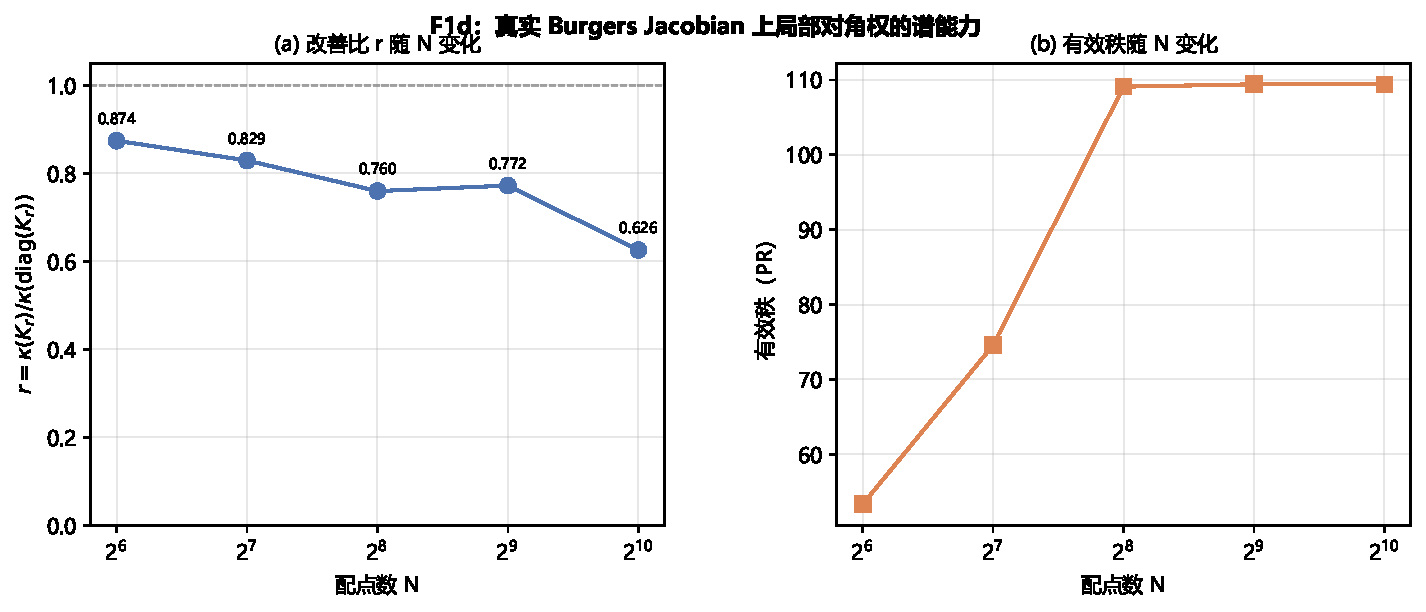
\includegraphics[width=0.92\textwidth]{fig_F1d_real_jacobian_zh.pdf}
\caption{实验 4.2：真实 Burgers 冻结 Jacobian（$\nu=.005$，近解好盆地）的 N 扫描。左：改善比 $r=\kappa^*_{\rm diag}/\kappa(R(K_r))$ 随 $N$ 变化，$N=64$--$512$ 时 $r\approx.76$--$.87$（多起点找到的改善 13\%--24\%），$N=1024$ 因双精度极限未纳入；右：有效秩（PR）随 $N$ 增大饱和于 $\sim109$，表明僵硬端方向共线主导。}\label{fig:f1d}
\end{figure}

\begin{figure}[ht]\centering
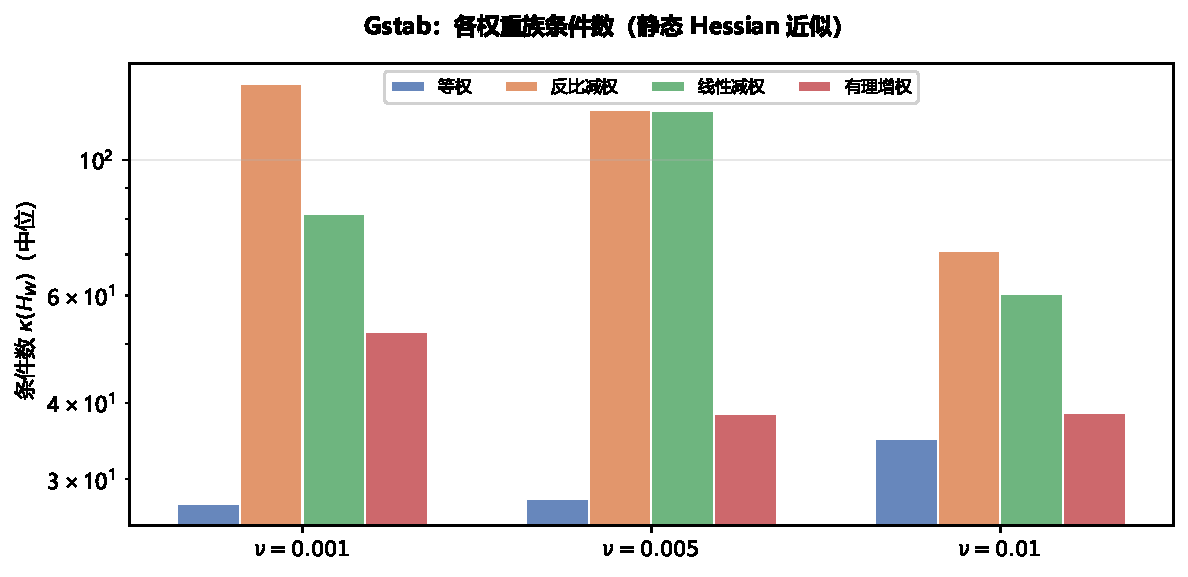
\includegraphics[width=0.85\textwidth]{fig_gstab_kappa_med_zh.pdf}
\caption{实验 4.3：训练过程完整 Hessian 谱端比 $\kappa=\lambda_{\max}/|\lambda_{\min}|$（代数极值口径，ARPACK/Lanczos 外缘估计，附录~\ref{app:repro}）的时间中位数（$n=22/\nu$，11 种子×2 clip）。减权族（down\_inv/down\_lin）在小粘性（.001/.005）下谱端比恶化 3--5 倍，rational 增权族与等权无显著差异。谱右端 $\lambda_{\max}$ 排序与梯度峰值排序一致（rational$\gg$uniform$>$down\_lin$>$down\_inv），但如 \S\ref{sec:theta-down} 所述，该尺度差异在 Adam 下被归一化吸收。}\label{fig:gstab}
\end{figure}

\begin{figure}[ht]\centering
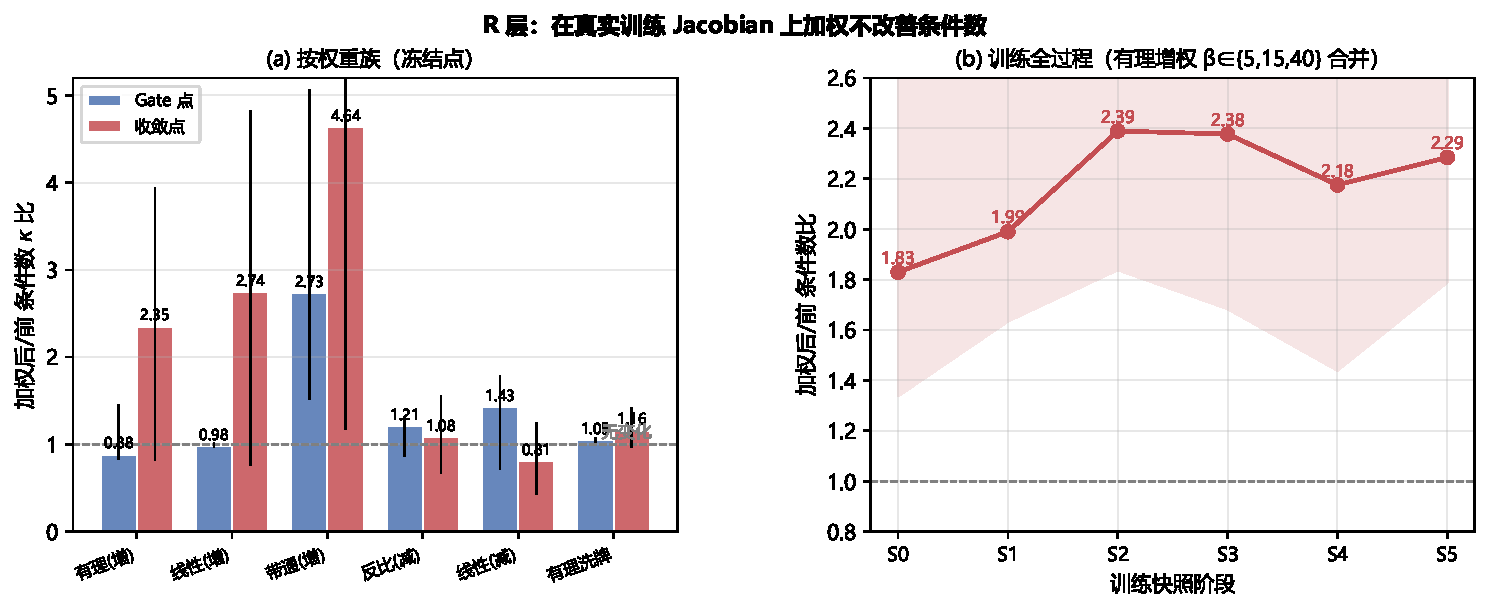
\includegraphics[width=0.95\textwidth]{fig_C2E3_kappa_train_zh.pdf}
\caption{实验 4.4：真实训练 Jacobian 上加权后/前条件数比 $\kappa(W^{1/2}JW^{1/2})/\kappa(JJ^\top)$。(a)~按权重族、Gate 与收敛两点（六族固定权）：增权族在收敛点恶化 $2.35$--$4.64$ 倍，减权族接近 $1$ 或略优；(b)~训练全过程（$S_0$--$S_5$，有理增权族 $\beta\in\{5,15,40\}$ 合并取逐快照中位，逐快照静态施加、不进入训练故不违反冻结 $W$ 划界）：比值中位 $1.83$--$2.39$，全程 $>1$。注意本图测冻结线性化 $H_{\rm lin}$，与实验 4.3 测完整 $H_{\rm lin}+H_{\rm nl}$ 不同，故 down\_lin 此处 $.81$（改善）与实验 4.3"恶化 3--5 倍"不矛盾。虚线 $=1$ 为无变化。}\label{fig:c2e3}
\end{figure}

\FloatBarrier

\section{一阶层面：优化动力学边界}\label{sec:theta}

本章研究空间加权通过加权梯度 $g_\W=J^\top\W r$ 进入单步更新后的动力学效应（冻结或外生缓变 $\W$ 口径；实验 5.3 的在线重算 $\W(\theta)$ 属类外经验观察，见实验 5.3 协议说明（表~\ref{tab:g1b}））。核心问题是：\emph{加权能否选择盆地？能否在好盆地内加速收敛？减权的作用区间是什么？}在本文研究的六族权重、$n=80$ 配对实验下，未观察到加权能显著改善盆地进入概率（uniform 命中率 $.613$ 反高于全部加权族）；加权的可观测效应局限于已进入的可精修盆地内的收敛速度调节。减权的真实定位是梯度尺度调节器（在本 testbed 上表现为训练早期尺度稳定；频谱失配下的终态收益见第~\ref{sec:crosseqn}~章），而非伪解盆地的逃逸手段。须注意，零解集不变（命题~\ref{prop:zero}）不蕴含吸引盆地不变（注记~\ref{rem:attractor}），故"加权不能选择盆地"是受控经验结论而非全称否定。本章先给出必要定义与机制 A 的代数层，再给出方向判据，最后以受控实验验证。

\subsection{加权训练流、盆地与两阶段}\label{sec:theta-flow}

\begin{definition}[加权训练流、吸引盆地与两阶段]\label{def:flow-basin}
固定权函数 $w(\cdot;\beta)$ 与优化器，参数迭代 $\theta_{k+1}=\mathcal A(\theta_k;w)$ 诱导离散流。对驻点 $\theta_B^\star$，其吸引盆地为 $B_{\W}(\theta_B^\star)=\{\theta_0:\lim_k\Phi_k^w(\theta_0)=\theta_B^\star\}$；\emph{真解盆地} $B(u^\star)=\{\theta_0:\liminf_k\|u_{\theta_k}-u^*\|_X<\rho_{\rm bas}\}$，其中 $\rho_{\rm bas}>0$ 是非线性局部吸收半径（未标定，不声称 $O(\nu^2)$ 标度）。好/伪解吸引域是 Phase~0 结束时刻的条件分类：落入 $B(u^\star)$ 为可精修吸引域，否则为伪解吸引域。

\textbf{两阶段与 Gate 停时}：\emph{Phase~0（盆地选择）}默认固定 $\beta=1$、施加 $\sigma$ 带宽课程，目标是以进入概率 $p_{entry}$ 落入真解盆地；\emph{Gate（关卡停时）}用不含真解的训练可观测量做一次性策略分流；\emph{Phase~1（盆地内精修）}固定已进入的盆地、调节 $\beta$ 与权族做局部收敛。盆地归属由 Phase~0 动力学决定、Phase~1 不再重新选择盆地（协议层面）；加权（增权或减权）前置到 Phase~0 能否改变盆地进入，正是实验 5.3/5.7 的检验对象，其结论（§\ref{sec:theta-down}）是经验结果而非协议的先验约定。
\end{definition}

\begin{remark}[零解集不变 $\ne$ 吸引盆地不变]\label{rem:attractor}
零残差集是代数对象、与 $w$ 无关（命题~\ref{prop:zero}）；吸引盆地是由向量场 $-\nabla L_\W$ 决定的动力系统对象，其几何与测度随 $w$ 改变。"保解但改优化"的精确含义是零残差集不变而盆地族被重塑。
\end{remark}

\subsection{机制 A：可精修盆地内的梯度能量再分配}\label{sec:theta-mechA}

\noindent\emph{定位说明。}机制 A（增权把梯度能量分配给难区）本身是 PINN 社区的常识性观察，本文的增量在于：在上述分层下严格区分，给出其权函数层确定性条件（C1/C2，有理权恒成立）与数据分布层对比度可分条件（C-Sep），并划定其失效边界。机制 A 不单独列为贡献，其价值在于为后续方向判据与减权假说的受控检验提供代数基础。

把配点分为激波带 $S$ 与光滑带 $O$（$|S|=O(\nu)N$）。下称\textbf{对比度可分}（C-Sep）：激波带的最低对比度不低于光滑带的最高对比度，即按残差相对幅值排序时两带完全不交叠；其概率松弛（C-Sep$^*$）只要求激波带的对比度分布对光滑带一阶随机占优。C-Sep 是"增权确实更多加到难区"的\emph{数据分布}前提：权函数只认识对比度 $t$、不认识"激波"，"$t$ 大 $\Leftrightarrow$ 难区"这座桥由 Phase~0 的训练动力学铺就，权函数本身保证不了。机制~A 分两层陈述。

\begin{proposition}[A0：名义再分配（权函数层确定）]\label{prop:mechA0}
\emph{权函数层（确定性）}：设 (C1)~$\partial_\beta w\ge0$；(C2)~$\partial_\beta w(t;\beta)$ 对 $t$ 非减；(C2$'$)~相对增长率 $\partial_\beta w/w$ 对 $t$ 非减。对有理权 $\partial_\beta w=t/(1+t)\in[0,1)$、$\partial_t(\partial_\beta w)=1/(1+t)^2>0$、$\partial_\beta w/w=t/(1+\beta t)$ 且 $\partial_t[\partial_\beta w/w]=(1+\beta t)^{-2}>0$，C1/C2/C2$'$ 对所有 $\beta\ge1,t\ge0$ 成立。\emph{数据分布层（对比度序）}：记 $S,O$ 上对比度为 $\{t_i\}$，严格版 (C-Sep) 为 $\min_{i\in S}t_i\ge\max_{i\in O}t_i$，概率版 (C-Sep$^*$) 只要求 $t|_S$ 对 $t|_O$ 一阶随机占优。则严格 C-Sep 下 $\partial_\beta\bar w_S\ge\partial_\beta\bar w_O\ge0$（仅需 C1/C2，\textbf{[确定]}）；且 $\bar w_S/\bar w_O$ 对 $\beta$ 非减（需 C2$'$；仅有 C1/C2 不充分，反例见附录，\textbf{[确定]}）；C-Sep$^*$ 下由 C2 非减与一阶随机占优的保序性\cite{Strassen1965}得 $\mathbb E_S[\partial_\beta w]\ge\mathbb E_O[\partial_\beta w]$，A0 在\emph{期望意义}成立（\textbf{[确定]}，给定占优假设）。严格 C-Sep 被违反时，A0 偏差由越序间隙 $\Delta=\max_{i\in O}t_i-\min_{i\in S}t_i$ 与越序点质量量化，越序越严重名义再分配越可能在期望上反转。
\end{proposition}
\begin{proof}[证明概要]完整证明见附录~\ref{app:proof}。
权函数层由 $\partial_\beta w\ge0$ 且对 $t$ 非减直接得到。数据分布层：严格 C-Sep 下 $S$ 上每个 $t_i$ 都大于等于 $O$ 上每个 $t_j$，由 $\partial_\beta w$ 非减得 $\partial_\beta w(t_i)\ge\partial_\beta w(t_j)$，取平均即得。概率版由一阶随机占优的保序性（Strassen 定理）：若 $F_S\le F_O$ 且 $f$ 非减，则 $\int f\,dF_S\ge\int f\,dF_O$。越序误差由分部积分 $\partial_\beta\bar w_S-\partial_\beta\bar w_O=-\int q'(t)(F_S-F_O)dt$，占优被违反的部分只来自正部 $(F_S-F_O)_+$。完整证明见附录~\ref{app:proof}。
\end{proof}

\begin{proposition}[A1：参数梯度能量实现（局部、条件性）]\label{prop:mechA1}
在 A0 上增加 (C3)~\emph{带内非自抵消}：$\langle\partial_\beta g_S,g_S\rangle\ge0$（带内行梯度 $J_i$ 的加权和不随权重增大而自相抵消）。则 $\partial_\beta\|g_S\|^2=2\langle\partial_\beta g_S,g_S\rangle\ge0$；而 $O$ 带 $t$ 有界、$\partial_\beta w$ 有界只给出上界 $\partial_\beta\|g_O\|^2\le\varepsilon_O\|g_O\|^2$（$\varepsilon_O:=2t_O^*(1+\eta_O\|g_O\|)$，$\eta_O$ 为带外非自抵消常数，推导见附录）；$O$ 带未加非自抵消假设，故不声明下界——其符号可正可负，只须被上界控制不爆炸。C3 是逐点可测的代数条件；实验 5.2 实测其在好/坏盆地均成立（$176$ 条探针记录全为正）——机制 A 在伪解盆地同样执行能量再分配，其不能纠正盆地归属的原因不在 C3，而在加速方向锁定于本盆地驻点方向 $d_B$ 而非真解方向 $d_*$（见下文的参照系讨论）。
\end{proposition}
\begin{proof}[证明概要]完整证明见附录~\ref{app:proof}。
$\partial_\beta\|g_S\|^2=2\langle\partial_\beta g_S,g_S\rangle$，由 C3 直接得非负。$O$ 带由 $\partial_\beta w\le1$（有理权）及 $t_O^*=\max_{i\in O}t_i$ 有界，给出 $\partial_\beta\|g_O\|^2\le2t_O^*(\|g_O\|^2+\eta_O\|g_O\|^3)$。完整推导见附录~\ref{app:proof}。
\end{proof}

\noindent\emph{计算直观。}增权在难区有效的代数本质是"把有限的梯度能量按对比度更多分配给难区"，它在权函数层是确定性恒等式；但能否兑现取决于数据分布（C-Sep）且必须已处在正确盆地内（C3）。增权是可精修吸引域内的精修手段，不是伪解吸引域的纠正手段。

\subsection{方向判据与对齐角的判别边界}\label{sec:theta-align}

\begin{definition}[两个目标方向与对齐角]\label{def:align}
区分两个目标方向：\emph{本盆地驻点方向} $d_B=\theta_B^\star-\theta$，其中 $\theta_B^\star$ 为当前所处盆地的驻点（定义同 \S\ref{sec:theta-flow}，坏盆地内 $\theta_B^\star$ 即伪解极小点）；\emph{真解方向} $d_*=\theta^*-\theta$，其中 $\theta^*$ 为真解的表示参数，即任一满足 $u_{\theta^*}=u^\star$ 的参数。好盆地内 $d_B=d_*$，坏盆地内二者不同。针对下降方向 $-g$ 定义余弦（$\cos>0$ 即下降朝向目标）：
\begin{equation}\label{eq:cos}
\cos\alpha(\beta;d)=-\frac{\langle g,d\rangle}{\|g\|\|d\|}\in[-1,1].
\end{equation}
\end{definition}

\begin{proposition}[增/减权的一阶方向判据]\label{prop:align}
梯度下降 $\theta^+=\theta-\eta g$，到目标 $d$ 的距离平方 $D=\tfrac12\|\theta-\theta_B^\star\|^2$ 的单步变化为
\begin{equation}\label{eq:step}
D^+-D=\eta\langle g,d\rangle+\tfrac{\eta^2}{2}\|g\|^2
=-\eta\|g\|\|d\|\cos\alpha+O(\eta^2).
\end{equation}
在 G-C 局部线性、小步长（$\eta\lambda_{\max}\ll1$，$\eta^2$ 项可略）与带内准均匀（C3$'$，激波带内对比度变异系数小）下：(i)~$\cos\alpha_S>c_0>0$（下降方向朝向目标）时，增大 $\beta$ 放大 $-g_S$ 与 $d$ 的对齐、\emph{加速靠近}（好盆地增权精修的充分条件）；(ii)~$\cos\alpha_S<-c_0<0$（下降方向背离目标）时，增大 $\beta$ 使 $\eta\langle g,d\rangle>0$、\emph{单步期望远离且随 $\beta$ 加快}；(iii)~减权（$w_S<1$）在尺度上压低该方向梯度贡献，仅是局部梯度尺度再平衡，不蕴含跨盆地逃逸。本判据对\emph{任意}目标方向 $d$ 成立，是纯一阶几何，不依赖 Burgers。
\end{proposition}
\begin{proof}[证明概要]完整证明见附录~\ref{app:proof}。
式~\eqref{eq:step} 由 Taylor 展开直接得到。在 C3$'$ 下 $\partial_\beta g_S=\bar c_\beta g_S+v_S$，$\|v_S\|\le\varepsilon_S\bar c_\beta\|g_S\|$，故 $\partial_\beta\langle g_S,d\rangle=\bar c_\beta\langle g_S,d\rangle+\langle v_S,d\rangle$，当 $|\cos\alpha_S|>\varepsilon_S$ 时符号由 $\langle g_S,d\rangle$ 决定。完整证明见附录~\ref{app:proof}。
\end{proof}

\begin{remark}[对齐角不能判别盆地好坏]\label{rem:align-emp}
命题~\ref{prop:align} 只需 G-C 局部线性与盆地内目标 $d$ 存在。代入两个参照系：好盆地 $d_B=d_*$、两参照系一致，增权沿 $d_B$ 加速即朝真解收敛；坏盆地沿 $d_B$ 加速等于沿 $d_*$ \emph{远离真解}。须注意两个目标方向都是 \emph{oracle 量}：$d_*$ 以真解 $\theta^*$ 为前提，$d_B$ 需以同盆地长训收敛解离线近似（实验 5.2 即以 $\beta_{\rm ref}=20$ 长训解构造），故本判据是分析工具而非可部署的在线检验。实验 5.2 的离线测量（冻结 Gate 点，$\beta=1$；数据见 \S\ref{sec:theta-exp}）表明：坏盆地对 $d_B$ 的 $\cos\alpha_S$ 中位 $+.0885$、$18/18$ 全部为正（范围 $[+.007,+.461]$）；好盆地对 $d_*$ 的 $\cos\alpha_S$ 中位仅 $+.0047$、$24/26$ 为正（范围 $[-.0045,+.594]$）（\textbf{[经验：坏 $n=18$、好 $n=26$]}）。同一探针的 C3 内积 $\langle\partial_\beta g_S,g_S\rangle$ 在全部 $176$ 条记录中均为正（含坏盆地），机制 A 的能量再分配在伪解盆地照常工作——失效的不是再分配本身，而是其加速方向被锁定在 $d_B$ 上。两类盆地对各自目标方向的对齐角都以正为主、好盆地中位反而更近零，$\cos\alpha_S$ 的符号分布对盆地好坏没有分离度——判别好坏是 Gate/实验 6.1 的职责（第~\ref{sec:methods} 章）。
\end{remark}

\subsection{减权的作用区间}\label{sec:theta-down}

\paragraph{盆地进入：减权逃逸假说被大样本配对证据拒绝。}
PINN 会收敛到训练残差很小但物理解错误的伪解吸引域、以及 continuation/重采样/缩域有助于规避伪解，这一现象本身已被建立\cite{Rohrhofer2022,WangPseudo2026}，本文不主张首次发现伪解或首次给出规避。早期 $n=3$ 的探索性实验曾观察到"伪解吸引域唯 down\_inv 可逃逸"，据此提出过\emph{空间减权逃逸}主张。该主张在 $n=80$ 配对实验 5.3 下被拒绝（表~\ref{tab:g1b}）：以同一 Phase~0 粗解配对（消除初始化混杂），等权 uniform 的可精修吸引域命中率 $.613$ 反高于全部加权族（$.388$--$.475$），净救回配对计数三族一致为负，Holm 校正后仅 down\_lin 显著（$p=.006$）（\textbf{[经验 $n=80$]}）。故事实整体不支持"减权提升盆地进入"，但不作减权在一切情形下都无法改变盆地归属的全称否定。

\paragraph{梯度尺度：Adam 下裁剪冗余，减权尺度被归一化吸收（实验 5.7，$n=20$ 配对，未做多重比较校正）。}
为分离减权的"尺度成分"与"方向成分"，设计族$\times$裁剪开关的 $2\times4$ 因子实验 5.7：同 Phase~0 协议下比较 grad\_clip$=1$（默认）与 grad\_clip$=0$（关闭）。结果：（i）关闭裁剪后零爆炸（blown$=0$，包括 $\nu=.001$、增权族 rational，其裁剪前梯度峰值高达 $7\times10^2$；实验 4.3 Stage-E 同配置实测中位 721）；（ii）裁剪开关在 $\nu=.005$ 未观察到对盆地进入率的影响（四族配对 McNemar $p=1.00$，进入率差异均在 $\pm.05$ 内）；（iii）显著信号仅出现在最硬端 $\nu=.001$、裁剪开启时 uniform 显著优于两个减权族（vs down\_inv $p=.016$，vs down\_lin $p=.039$），复现实验 5.3；裁剪关闭时族间差异不显著（全量统计见 \S\ref{sec:theta-exp}、图~\ref{fig:g1c}）。机制：Adam 的二阶矩归一化 $\sqrt{\hat v_t}$ 已自适应吸收原始梯度范数的尺度效应，显式 L2 裁剪与空间减权对 $g_{\text{peak}}$ 的压低在 Adam 下不传导到优化轨迹（\textbf{[经验 $n=20$]}）。

\paragraph{盆地内 lr 裕度：线性减权 down\_lin 推高有效训练上限（实验 5.8，$n=8$ 配对，方向性证据）。}
从 Gate 点（好盆地内）出发，固定步长 Adam 跑 500 步。爆炸意义上的稳定 lr 极宽：lr$\le.05$ 四族全不爆炸，lr$=.1$ 仅 rational（增权）爆炸率 $50\%$、减权族 $12.5\%$、uniform $0\%$。但以终态 $L_2<.06$（好盆地阈值）定义的\emph{有效训练 lr 上限}显示：down\_lin 中位 $.002$ 高于 uniform $.001$（配对 Wilcoxon 精确双侧 $p=.0625$、渐近 $\approx.043$；$n=8$ 配对中仅 $5$ 对非零差，方向一致但未达 $.05$ 显著）。在宽松阈值 $L_2<.1$ / $<.2$ 下 down\_lin 的优势更明显（中位 $.0035$ / $.005$，其他族 $.001$--$.002$；全量统计见 \S\ref{sec:theta-exp}、图~\ref{fig:b1b}）。结论：线性减权在已进入好盆地后中位有效训练 lr 上限约推高一倍，但该效应小、仅在 down\_lin 一族呈边缘趋势（精确 $p=.0625$），且不改变盆地进入（\textbf{[经验 $n=8$，seed 10/15/20 无好盆地被排除]}）。

\paragraph{固定步长 L-BFGS 对照：四族终态无显著差异（实验 5.9，$n=5$--$8$，阴性结果、方向性证据）。}
为检验"Adam 归一化吸收尺度"是否为减权无盆地进入收益的原因，设计固定步长 L-BFGS 对照（\texttt{line\_search\_fn=None}，无 Adam 式逐坐标归一化，割线阵仅由历史加权梯度构造，属准入类内）：Adam 200 步预热 + L-BFGS 500 outer steps。在 $\nu=.005$（$n=8$）与 $\nu=.001$（$n=5$，其余 seed 无好盆地）下，四族终态 $L_2$ 均无显著差异，所有配置零爆炸（全量统计见 \S\ref{sec:theta-exp}）。结论：即使移除 Adam 归一化，空间减权在好盆地内也不产生可检测的终态差异——梯度尺度不是盆地内优化的瓶颈（\textbf{[经验]}）。

\paragraph{梯度曲线：减权压低峰值的几何效应真实存在（$n=8$，归入实验 5.9）。}
从 Gate 点出发、lr$=10^{-3}$、逐 50 步记录裁剪前 $\|g\|_2$，500 步内排序稳定：rational（$27$--$63$）$\gg$ uniform（$3$--$6$）$>$ down\_lin（$.2$--$.8$）$>$ down\_inv（$.1$--$.4$）。减权对梯度尺度的压低效应真实且全程不收敛趋同，但如上述，该效应在 Adam 下被归一化吸收、在固定步长 L-BFGS 下也不改变终态。

\medskip
\noindent\textbf{小结。}空间减权（尤其线性减权 down\_lin）在已进入好盆地后有轻微的 lr 裕度稳定效应（有效训练 lr 上限中位推高一倍，精确双侧 $p=.0625$、渐近 $\approx.043$，为未达 $.05$ 显著的边缘趋势），但其尺度成分被 Adam 归一化吸收、固定步长下也不改变终态；它不帮助进入盆地、不逃逸伪解、不是预条件器。减权的作用窗口被严格限定在"盆地内、线性减权、lr 裕度"这一窄区间内。

\subsection{实验验证}\label{sec:theta-exp}

\noindent\textbf{优化器与准入类声明。}本章全部主实验（实验 5.1/5.2、实验 5.3、实验 5.4/5.5/5.6、实验 6.1）的 Phase~0 与 Phase~1 均使用固定步长 Adam（$\beta_1=.9,\beta_2=.999$，无基于 $L_\W$ 的线搜），属定义~\ref{def:admit} 的准入类内算法，引理~\ref{lem:linrec} 覆盖。实验 4.3 的 Stage-B2 为固定步长 L-BFGS 对照实验（PyTorch \texttt{LBFGS}，未设置 \texttt{line\_search\_fn}，即不做 Armijo 回溯；割线阵由历史加权梯度构造，属信息集 $\mathcal I_k$ 内的间接量，不读取 $L_\W$），亦在准入类内。本文未使用带线搜的 L-BFGS 或任何直接读取 $L_\W$ 的优化器。

\paragraph{实验 5.1/5.2：机制 A 的方向核验（冻结点确定性自检）。}
冻结 Gate 点、同 $\theta$ 同 $r$ 仅改 $\beta$，激波带梯度能量占比 $\eta_{gate}$ 随 $\log\beta$ 单调：冻结点自检脚本在四个粘度上 Spearman 秩相关全为 $+1$，实验 5.1 跨宽度/深度/配点共 7 个配置方向不变（图~\ref{fig:r1g3}，全量数据见附录表~\ref{tab:app-r1}）。\emph{C-Sep 直接测量}：在同冻结点上计算激波带 $S$（$|x|<3\nu$）与光滑带 $O$ 的对比度 $t=|r|/\mathrm{median}|r|$，$N=128$--$512$ 时带间中位比 $\mathrm{median}(t_S)/\mathrm{median}(t_O)=38$--$45$（严格 C-Sep 比值 $\min(t_S)/\max(t_O)=0.72$--$8.88$，$N=512$ 时严格版不成立但中位比仍达 $38$），即机制 A 的数据前提在僵硬端冻结点上经验成立。须说明实验 5.1 的证据级别：这是在\emph{同一冻结点}上对确定性函数 $\beta\mapsto\eta_{gate}$ 的秩单调性自检（机制核验），只要 C1/C2 与 C-Sep 在该点成立它即恒为 $+1$，\emph{不是}跨种子的经验统计、也不构成训练收益证据；其作用是核验命题~\ref{prop:mechA0}/\ref{prop:mechA1} 的代数层在实测冻结点成立。该单调性既不蕴含最终收敛，也不判别盆地好坏。

\paragraph{实验 5.2 对齐角探针：$\cos\alpha_S$ 对盆地好坏无分离度。}
同一实验 5.2 探针在冻结 Gate 点离线测量激波带对齐角 $\cos\alpha_S=-\langle g_S,d\rangle/(\|g_S\|\|d\|)$，目标方向 $d$ 取同盆地 $\beta_{\rm ref}=20$ 长训收敛解构造的目标方向（离线 oracle，非无真解部署量），共 $11$ seeds $\times$ $4$ 粘度 $\times$ $4$ 档 $\beta$、$176$ 条记录。$\beta=1$ 下（$\beta=3/10/40$ 几乎相同）：坏盆地（$n=18$，对本盆地伪解驻点方向 $d_B$）$\cos\alpha_S$ 中位 $+.0885$、$18/18$ 全正（范围 $[+.007,+.461]$）；好盆地（$n=26$，对真解方向 $d_*$）中位 $+.0047$、$24/26$ 为正（范围 $[-.0045,+.594]$）。两类盆地的对齐角符号分布无分离度，这是注记~\ref{rem:align-emp} 判别边界结论的经验来源。

\begin{figure}[ht]\centering
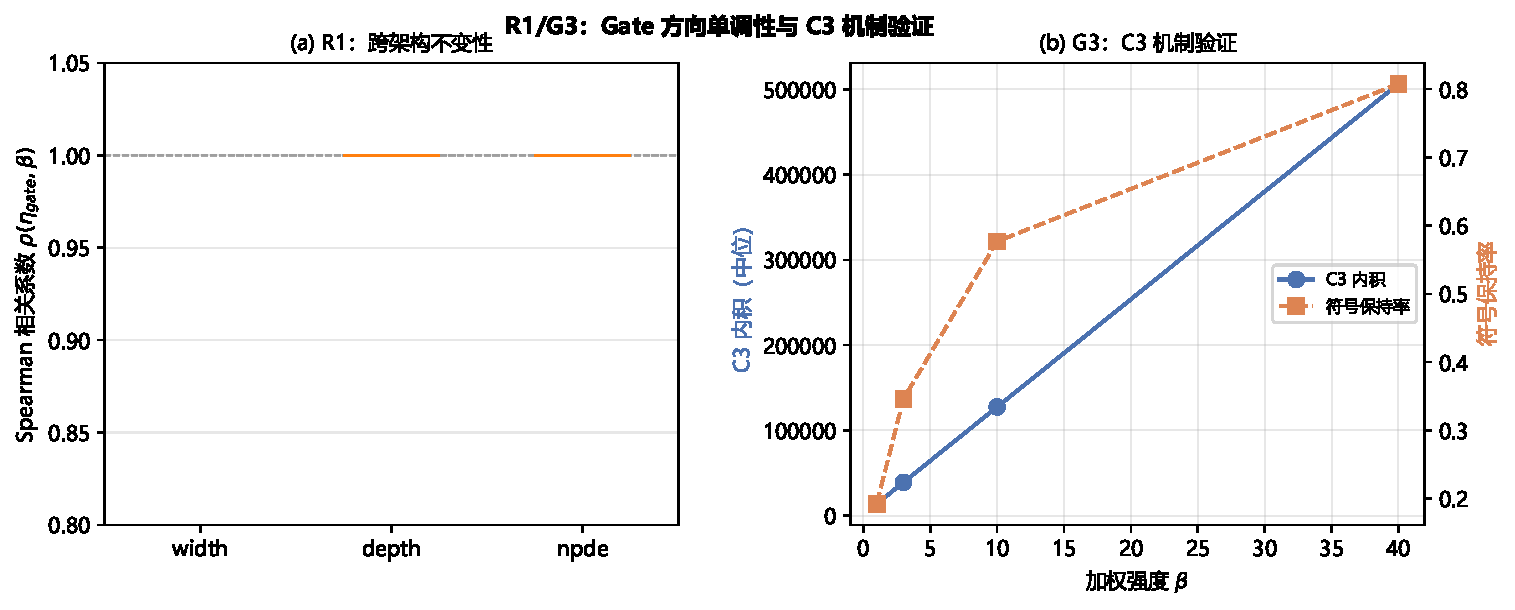
\includegraphics[width=0.92\textwidth]{fig_R1_G3_monotonicity_zh.pdf}
\caption{实验 5.1/5.2：机制 A 的方向核验。左（实验 5.1）：跨架构（宽度/深度/配点数）的 Gate 方向量 $\eta_{gate}$ 对 $\beta$ 的 Spearman 秩相关系数，全部 $\rho_s=+1$（冻结点确定性自检，与架构无关）；右（实验 5.2）：好盆地内 C3 内积 $\langle\partial_\beta g_S,g_S\rangle$ 中位随 $\beta$ 单调增大（$1.4\times10^4\to5.1\times10^5$，蓝线，左轴；$176$ 条探针记录均为正，弱条件 C3 在冻结 Gate 点逐点成立）；方向判据定号条件达成率（$\cos\alpha_S>\varepsilon_S$ 的配置占比，橙线，右轴）随 $\beta$ 由 $.19$ 升至 $.81$（$\varepsilon_S$ 随 $\beta$ 减小，C3$'$ 随之增强）。}\label{fig:r1g3}
\end{figure}
\paragraph{实验 5.3：盆地进入与减权假说检验（$n=80$ 配对）。}
为研究权重对盆地\emph{进入}的影响，本实验将权重族前置到 Phase~0 并在线重算 $\W=\W(r(\theta))$：同一 $(\nu,\text{seed})$ 下分别以四族（uniform 复用 G1 缓存；down\_inv/down\_lin/rational 各 $\beta=10$）独立跑 Phase~0 的 $K=4$ 多起点选优（$K=4$ 起点为同一 $(\nu,\text{seed})$ 下以 4 个连续子种子 $s,s{+}1,s{+}2,s{+}3$ 各自独立重训的 Phase~0 粗解：全新初始化、非同一轨迹重启；基础种子按 5 等距、子种子段互不重叠；跨族配对共享子种子，初始化方向相同、仅权重族不同），比较四族 Phase~0 末 $L_2$ 落入真解邻域（绝对阈值 $L_2<.06$，与族无关）的命中率并做同种子配对 McNemar。\emph{协议声明}：Phase~0 权重前置时对比度场 $t=|r|/\mathrm{median}|r|$ 随训练在线重算（$\W=\W(\theta)$），属\emph{探测性设计}、超出原则~II 的冻结 $\W$ 准入类；该在线重算设计同时也是实践者部署自适应权重的真实方式，其负结果用于探测 Gate 前盆地进入边界，与 Gate 后冻结 $\W$ 的原则~II 结论互补而非冲突。原则~II 严格结论仅覆盖 Gate 后冻结 $\W$ 的 Phase~1 精修。四族命中率与配对检验统计见表~\ref{tab:g1b}。

\begin{table}[ht]\centering\small\renewcommand{\arraystretch}{1.2}
\begin{tabular}{lccccc}
\toprule
权重族 & 命中率 & 配对差（uniform$-$族） & 95\% CI$^\dagger$ & McNemar $p$ & Holm 校正后$^\ddagger$\\
\midrule
uniform & $.613$ & -- & -- & -- & --\\
rational & $.463$ & $+.150$ & $[+.003,+.297]$ & $.065$ & 不显著\\
down\_inv & $.475$ & $+.138$ & $[+.015,+.260]$ & $.043$ & 不显著\\
down\_lin & $.388$ & $+.225$ & $[+.086,+.364]$ & $.002$ & $p=.006$（显著）\\
\bottomrule
\end{tabular}
\caption{实验 5.3：$n=80$ 配对（4$\nu$×20 种子，K=4 选优口径），各权重族的可精修吸引域命中率。配对差为 uniform 命中率减加权族命中率（正值表示 uniform 更优）。三族净救回均为负。$^\dagger$95\% CI 为单检验口径（未做多重比较校正），三族 CI 全为正（方向高度一致，uniform 命中率均高于加权族），这是比单个检验显著更强的方向一致性证据；$^\ddagger$Holm 校正后（3 重比较，族错误率控制）仅 down\_lin 显著（$p=.006$），down\_inv 与 rational 点估计方向一致但校正后 $p>.05$。按 $\nu$ 分层：小粘性（.001）差异最大（配对差 $+.25$--$.35$），过渡粘性（.01）方向不一致。结论：在 $n=80$ 配对下未观察到减权能显著提高盆地进入概率，uniform 命中率反高于全部加权族；不作全称否定。}\label{tab:g1b}
\end{table}

\noindent\emph{阈值稳健性（N6）}：将好盆地阈值 $\tau$ 在 $[.03,.08]$ 内扰动重算配对 McNemar，down\_lin 在 $\tau\in[.05,.08]$ 时 Holm 校正后仍显著（$p=.001$--$.032$），$\tau=.03/.04$ 时最少族好盆地仅 $18/80$、检验功效不足；主结论在常用阈值区间稳健。

\paragraph{实验 5.4/5.5/5.6：可精修盆地内加权强度的经验观察（$n=11$ 全量，描述性）。}
薄激波端存在事后最优 $\beta$（逐种子最优 $\beta^*$ 在实验 5.4 的 $\nu=.001/.003/.005/.01$ 上中位为 $1/5/20/10$，在实验 5.5 的 $\nu=.005/.1/.5$ 上中位为 $8/1/3$），但单种子散布大（$1$--$100$）、不随粘度单调，三固定强度终态区间重叠、无一致排序（图~\ref{fig:e1heat}；逐格全量数据见附录表~\ref{tab:app-e1}、表~\ref{tab:app-r2}）；$\nu=.001$、$\beta\ge5$ 全部塌缩到同一失败态（热力图中为中位 $\approx.573$ 的深红格；固定强度比较中已排除，下述 $g_{\rm post}$ 统计中保留）。光滑端曲线近平坦、增益落误差地板。实验 5.6 退化扫描（1584-run）表明：机制性增益主要集中在 MLP 主干的激波带内误差口径（$\nu=.01/.03$ 的逐种子最优中位 gain 约 $10.4/3.9$；总 $L_2$ 口径为 $4.43/1.40$）；光滑端绝对误差进入 $10^{-6}$ 地板，$\nu\ge.3$ 时 C-Sep 分区失去 S/O 语义，相对增益不再按物理收益解释；固定高带宽 Hi 在 $\nu\ge.3$ 相对 MLP/Match 明确失配。事后最优 $\beta$ 只是描述性可达上界：实验 5.4 薄激波端 $n=44$ 格（$4$ 粘度 $\times$ $11$ 种子，含失败态格）上，事后最优相对增益 $g_{\rm post}=\big(L_2(\beta{=}1)-\min_\beta L_2\big)\big/L_2(\beta{=}1)$ 中位仅 $.08$、IQR $[0,.59]$、范围 $[0,.97]$，且 $\beta^*$ 对 $\nu$ 非单调，不构成可部署策略，不推荐单点 $\beta^*(\nu)$。

\paragraph{实验 5.7：裁剪开关因子（$n=20$ 配对，分离尺度与方向成分）。}
族$\times$裁剪开关 $2\times4$ 因子设计。关闭裁剪后零爆炸（含 $\nu=.001$、rational 裁剪前峰值 $7\times10^2$）；$\nu=.005$ 未观察到裁剪开关对盆地进入率的影响（四族 $p=1.00$）；显著信号仅在 $\nu=.001$、裁剪开启时 uniform 优于两个减权族（$p=.016$/.039），复现实验 5.3。Adam 二阶矩归一化已吸收梯度尺度，显式裁剪与减权对 $g_{\text{peak}}$ 的压低不传导到优化轨迹（\textbf{[经验 $n=20$]}；图~\ref{fig:g1c}）。

\begin{figure}[ht]\centering
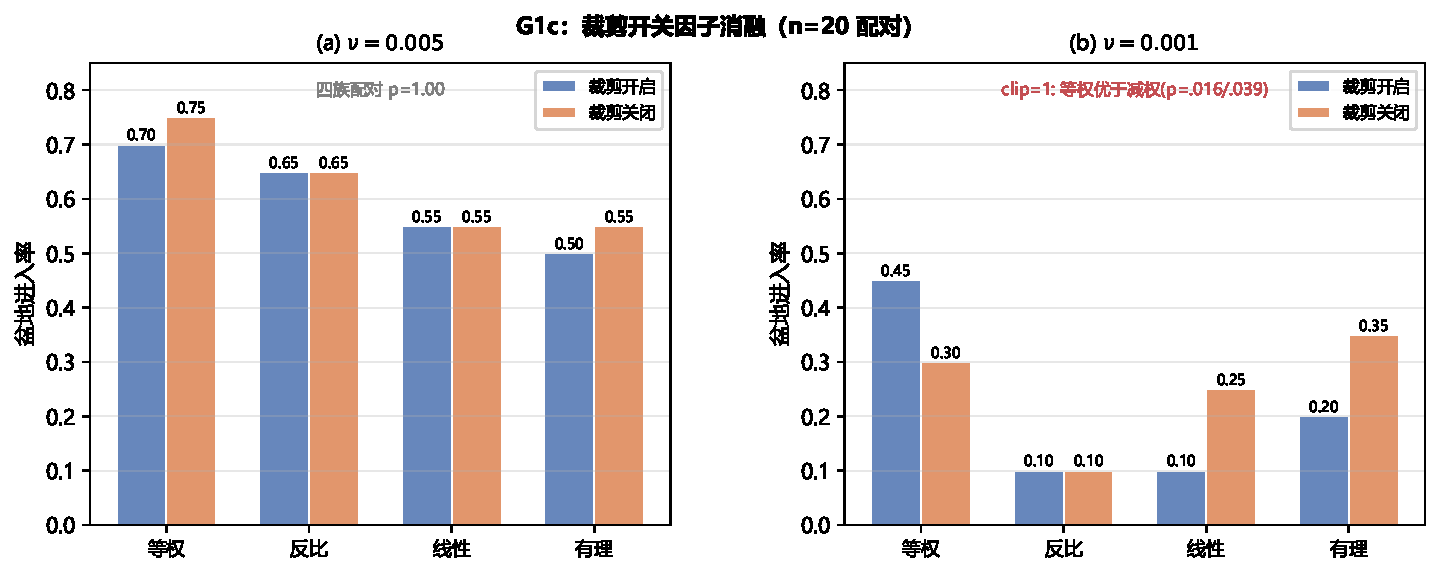
\includegraphics[width=0.92\textwidth]{fig_G1c_clip_zh.pdf}
\caption{实验 5.7：裁剪开关因子消融（$n=20$ 配对，K=4 选优口径）。左：$\nu=.005$，未观察到裁剪开关对盆地进入率的影响（四族配对 McNemar $p=1.00$）；右：$\nu=.001$，裁剪开启时 uniform 显著优于两个减权族（$p=.016$/.039），裁剪关闭时族间差异不显著。关闭裁剪后零爆炸。}\label{fig:g1c}
\end{figure}

\begin{figure}[ht]\centering
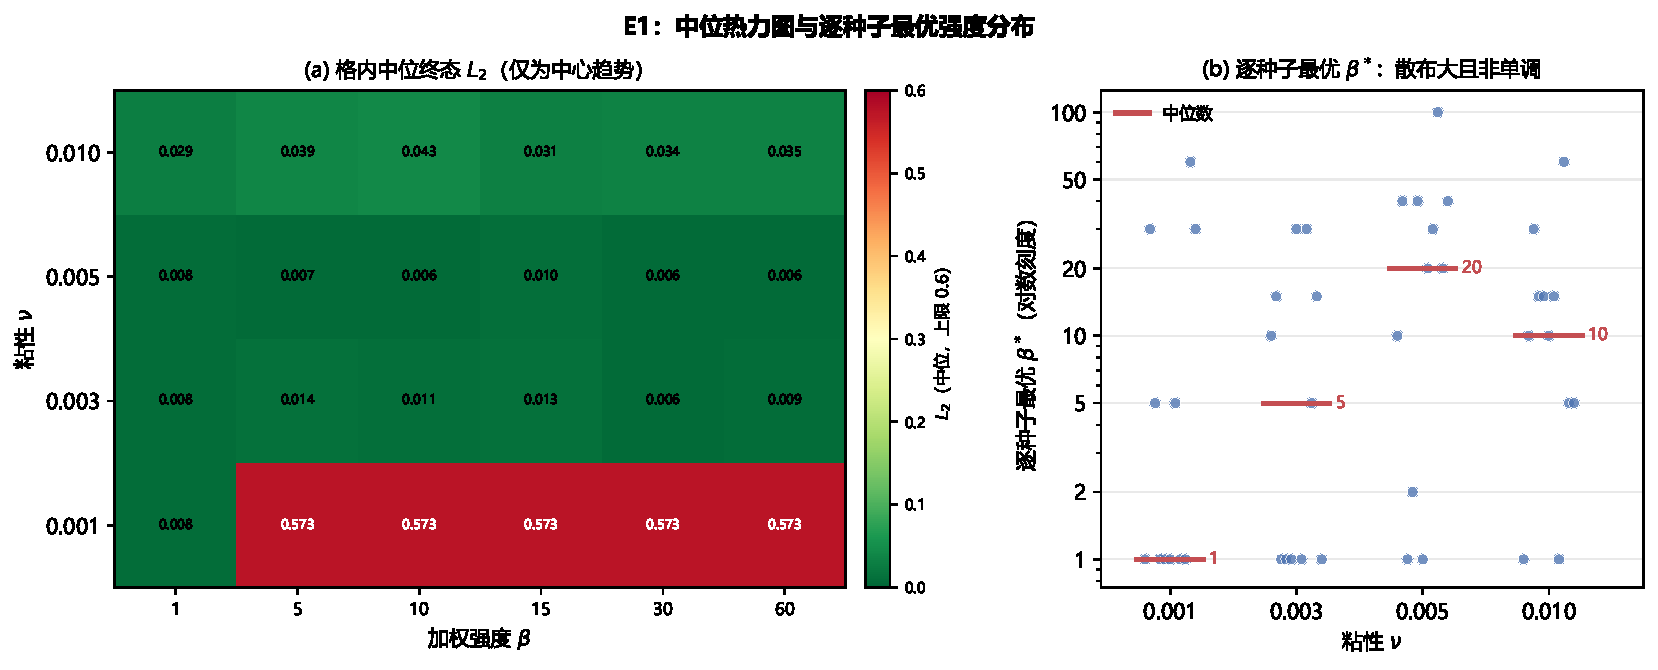
\includegraphics[width=0.98\textwidth]{fig_E1_beta_nu_heatmap_zh.pdf}
\caption{实验 5.4：左：格内中位终态 $L_2$（$n=11$，仅显示跨种子中心趋势）随加权强度 $\beta$ 与粘性 $\nu$ 的变化；右：逐种子最优 $\beta^*$ 分布（各 $\nu$ 中位 $1/5/20/10$、整体中位 $10$，范围 $[1,100]$）。薄激波端存在事后最优 $\beta$，但逐种子散布大且不随粘度单调；格内中位数最小点与逐种子 $\beta^*$ 中位数不必一致，本图不用于识别可部署策略。大粘性端曲线近平坦、相对增益落误差地板。左图仅显示四个粘度公共的 $6$ 档 $\beta$（$\nu=.005$ 的加密档见附录表~\ref{tab:app-e1}）；$\nu=.001$、$\beta\ge5$ 各深红格为全部种子塌缩到的同一失败态（格内中位 $\approx.573$）。}\label{fig:e1heat}
\end{figure}

\paragraph{实验 5.8/5.9：盆地内 lr 裕度与优化器对照。}
\emph{实验 5.8（$n=8$）}：Gate 点出发固定步长 Adam，lr 网格 $5\times10^{-4}$--$10^{-1}$。爆炸意义稳定 lr 极宽（$\le.05$ 全不炸），但以 $L_2<.06$ 定义的有效训练 lr 上限：down\_lin 中位 $.002$ 高于 uniform $.001$（配对 Wilcoxon 精确双侧 $p=.0625$、渐近 $\approx.043$，方向一致但未达 $.05$ 显著），down\_inv 有趋势（$p=.180$），rational 反而更低（$p=.109$）。其中 down\_inv、rational 两对及下文实验 5.9 的全部 $p$ 值为正态渐近近似（非零差仅 $2$--$5$ 对，精确枚举不适用）。线性减权把有效 lr 上限中位推高一倍，但效应小、仅 down\_lin 呈边缘趋势、不改变盆地进入（图~\ref{fig:b1b}）。

\emph{实验 5.9（固定步长 L-BFGS 对照）}：Adam 200 步预热 + L-BFGS 500 outer steps（\texttt{line\_search\_fn=None}，属准入类内）。$\nu=.005$（$n=8$）四族终态 $L_2$ 配对 $p=.069$--$.161$（无显著差异）；$\nu=.001$（$n=5$）$p=.345$--$.686$。即使移除 Adam 归一化，减权在好盆地内也不产生可检测终态差异——梯度尺度不是盆地内优化瓶颈。

\emph{梯度曲线观察（$n=8$）}：500 步内 $\|g\|_2$ 排序稳定：rational $\gg$ uniform $>$ down\_lin $>$ down\_inv，减权压低峰值的几何效应真实但不改变终态。三者共同结论见 \S\ref{sec:theta-down}。

\begin{figure}[ht]\centering
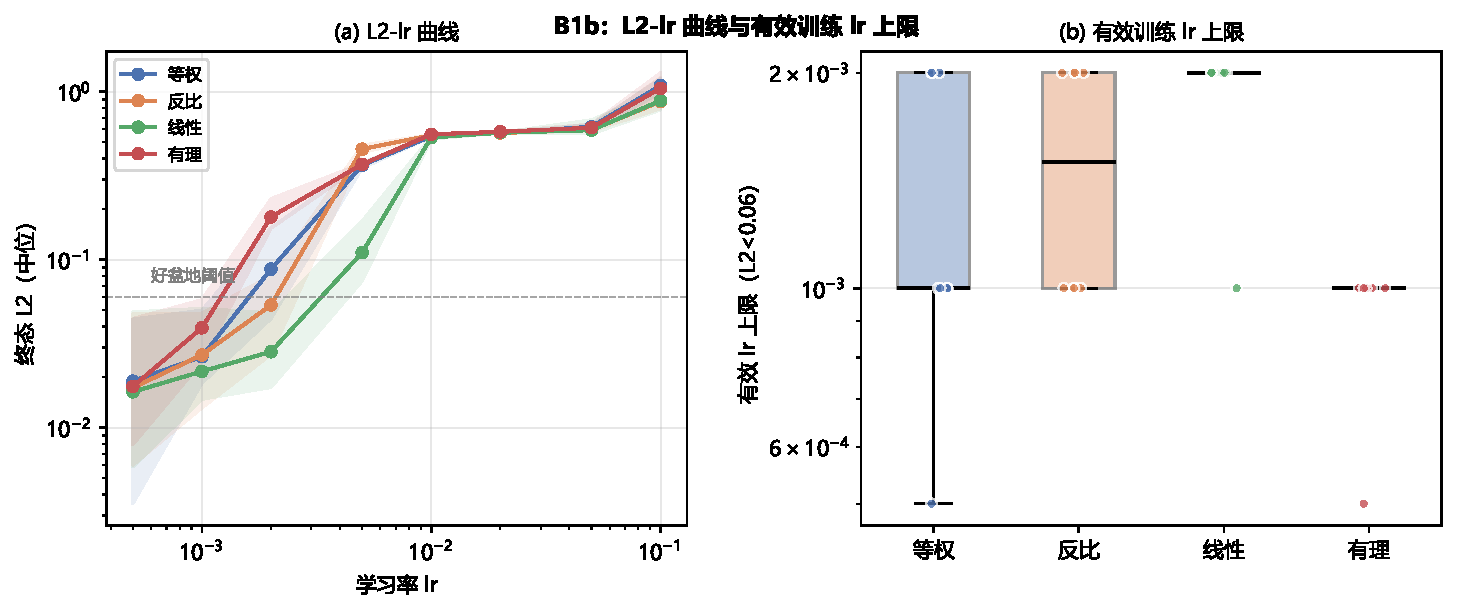
\includegraphics[width=0.92\textwidth]{fig_B1b_lr_curve_zh.pdf}
\caption{实验 5.8：盆地内 lr 裕度（$n=8$ 配对，从 Gate 点出发固定步长 Adam 500 步）。左：终态 $L_2$ 随 lr 的变化（中位$\pm$IQR），lr$\ge.01$ 四族全部平台化（离开好盆地），虚线为好盆地阈值 $L_2=.06$；右：以 $L_2<.06$ 定义的有效训练 lr 上限箱线图，线性减权 down\_lin 中位 $.002$ 高于等权 uniform $.001$（配对 Wilcoxon 精确双侧 $p=.0625$、渐近 $\approx.043$，方向一致但未达 $.05$ 显著的边缘趋势）。}\label{fig:b1b}
\end{figure}

\noindent\textbf{三条经验事实共同勾画出空间加权在一阶层面上的"作用窗口"：已进入的可精修盆地 $\times$ 存在局域刚性对比度。}在本文研究的六族权重与 $n=80$ 配对下，窗口之外——伪解吸引域、或本已光滑的问题——空间加权未观察到显著的盆地进入改善，也不带来系统收益。这是受控经验结论，不排除其他权重族或自适应策略在盆地选择上的作用。

\FloatBarrier

\section{无真解判别方法学边界}\label{sec:methods}

两阶段流程在部署时不允许使用真解，故 Gate 停时只能依赖训练可观测量。本章先给 Gate 的形式，再用可识别性分析说明"残差/损失自评估标量为什么不够、需要什么空间结构量"，最后以实验 6.1 实验验证。

\subsection{Gate 停时与两类判定}\label{sec:gate}

\begin{definition}[Gate 停时与 Gate-A/Gate-B]\label{def:gateAB}
Gate 是 Phase~0 结束处的\emph{一次性}策略选择器，其输入为训练可观测量 $Z_k$（不含真解）。\textbf{Gate-A}（确定性触发规则，操作定义）：同时满足 (A-i)~训练窗内损失相对下降率低于阈值、梯度范数进入平台；(A-ii)~冻结探针的 $\eta_{gate}$ 对 $\beta$ 单调（机制 A 的 A0/A1 聚合成立）；(A-iii)~三表示器（Hi/Match/MLP，见 \S\ref{sec:theta-exp}）粗解在激波带外一致。三条同时成立规定流程上"何时切入 Phase~1"，是 Gate 的设计与停时定义，\emph{不是}关于"盆地客观好坏"的数学充分条件——三条衡量的是训练状态与表示一致性，盆地真伪仍由 Phase~1 能否精修到真解事后判定。\textbf{Gate-B}（经验、高概率）：当 Gate-A 不全部可判时，用多变量判别器 $\mathcal G_B(Z)$ 估计盆地归属，其灵敏度、特异度与留一总准确率由跨粘度留一实验估计。Gate-B 是\emph{一次性分流}：判坏即多起点重启，不做减权逃逸；判好即进入 Phase~1、选定后不中途切换。本篇把 Gate-B 的留一功效仅作为\emph{可行性证据}（样本只覆盖一维稳态 Burgers 的所测粘度网格），不构成跨方程部署承诺。
\end{definition}

\begin{remark}[为何不能用训练损失自评估选盆地]\label{rem:noground}
伪解吸引域同样是局部极小、其训练损失可降到与可精修吸引域相当，故"训练损失小"不蕴含"盆地好"；命题~\ref{prop:bayes} 将证明残差/损失自评估类固定单投影在两类边缘分布完全重叠时退化为机会水平、部分重叠时也受该标量 Bayes 误差与阈值类限制约束，Gate 必须引入不与残差自评估等价的空间结构量或多表示器交叉验证。
\end{remark}

\subsection{可识别性：固定单投影标量的 Bayes 误差与四点反例}\label{sec:open}

\begin{proposition}[固定单投影标量字典的可识别性下界（条件性）]\label{prop:bayes}
(i)~\textbf{Bayes 下界}：对任意判别器 $\mathcal G$，$\mathrm{Err}(\mathcal G)\ge\mathrm{Err}_B=\tfrac12\int\min(p_G,p_B)\,dZ$（等先验）；只有当两类条件分布在 $Z$ 上几乎处处可分时 $\mathrm{Err}_B=0$。
(ii)~\textbf{固定投影族标量的可识别性下界（条件性）}：若判别器只允许使用固定投影族 $\{t^\top z\}$ 中的标量（典型为残差/损失自评估量，如朴素训练损失、朴素激波带误差；携带空间对比度结构的量不在本款覆盖内），由 Cram\'er--Wold 定理，该族不能区分边缘分布相同的两类，记两类在该标量上的条件密度为 $p_G,p_B$。则：(a)~不限判别形式时，该标量上的最优错误率是其 Bayes 误差 $\mathrm{Err}_B(z)=\tfrac12\int\min(p_G,p_B)\,dz$（重叠积分），它在两类\emph{完全重叠}（$p_G=p_B$ 几乎处处）时等于机会水平 $\tfrac12$，在\emph{部分重叠}时可严格小于 $\tfrac12$——故"分布重叠"本身\emph{不}蕴含机会水平下界，只有"完全重叠（边缘分布相同）"才蕴含；(b)~若进一步限定为"该标量与单一固定阈值比较"的\emph{阈值规则}（受限类），其最优错误率 $\mathrm{Err}_{\rm thr}^*$ 一般满足 $\mathrm{Err}_{\rm thr}^*\ge\mathrm{Err}_B(z)$，等号当且仅当似然比 $p_B/p_G$ 关于该标量单调；似然比非单调时（如一类为双峰）任何单阈值规则严格次优。该结论是条件性的——若某标量使两类近似可分，$\mathrm{Err}_B$ 与 $\mathrm{Err}_{\rm thr}^*$ 都可接近零，故不声称任何标量在一切情形都不可用。
(iii)~\textbf{四点反例（质心重合、固定投影族不可精确分离）}：取四点 $G=\{(-\tfrac12,-\tfrac12),(\tfrac12,\tfrac12)\}$、$B=\{(-\tfrac12,\tfrac12),(\tfrac12,-\tfrac12)\}$（教科书 XOR）。两类质心重合于原点、任意仿射线性函数在两类上均值相同，故\emph{不存在零错误的仿射线性分离器}；全体仿射阈值规则的最小错误率（对 $f$ 与阈值取最小）为 $\tfrac14$（例如取 $f(z)=z_1+z_2$，$G$ 上值为 $\{\pm1\}$、$B$ 上恒为 $0$，最优阈值错误率 $\tfrac14$；$ab=0$ 的单坐标退化情形两类取值多重集相同、错误率恰为 $\tfrac12$）。注意单一标量上两类边缘\emph{不一定}完全重叠——上述 $f(z)=z_1+z_2$ 的边缘分布不同，可达 $\tfrac14$ 错误率，故不能由单坐标不可判别推出"任一单标量判别都恰为机会水平"；正确的结论是"不可精确（零错误）分离"。必须引入交互特征 $q=z_1z_2$（或任一非线性判别器）方可达零错误。一个 $n=400$ 的\emph{合成四点探针}（非实验 6.1 真实样本，仅作机制说明）复现同一分界：单坐标 AUC $=.542$、朴素\emph{纯线性}两坐标 AUC $=.566$（近机会水平），加入结构交互量 $z_1z_2$ 后 AUC 升至 $1.000$。
\end{proposition}
\begin{proof}[证明概要]完整证明见附录~\ref{app:proof}。
(i) 由 Bayes 误差的定义直接得到。(ii)(a) 由 $\mathrm{Err}_B(z)=\tfrac12\int\min(p_G,p_B)dz$，当 $p_G=p_B$ 时 $\min=p_G$，积分 $=1/2$；部分重叠时 $\min<p_G$ 在重叠区外，积分 $<1/2$。(ii)(b) 阈值规则的最优错误率是在受限类上的最小值，受限类的最小值 $\ge$ 无约束类的最小值（Bayes 误差）；等号当且仅当 Bayes 规则本身属于阈值类，即似然比单调。(iii) 直接验证：对任意仿射线性函数 $f(z)=az_1+bz_2+c$，$f$ 在 $G$ 上的两个值为 $c-(a+b)/2$ 和 $c+(a+b)/2$，在 $B$ 上为 $c+(-a+b)/2$ 和 $c+(a-b)/2$。两类均值均为 $c$（质心重合），故均值差为零。但两类边缘分布\emph{不一定}相同：取 $a=b=1$、$c=0$ 时，$G$ 上值为 $\{\pm1\}$、$B$ 上恒为 $0$，最优阈值错误率为 $1/4$。一般地，全体仿射阈值规则的最小错误率为 $1/4$：零错误不可能（两类均值同为 $c$，严格分离要求两类均值分居阈值两侧，矛盾），错误率为 $1/4$ 的整数倍（四点各占总质量 $1/4$），而 $f=z_1+z_2$ 达到 $1/4$；$ab=0$ 的单坐标退化情形两类取值多重集相同、错误率恰为 $1/2$。交互量 $q=z_1z_2$ 在 $G$ 上为 $+1/4$，在 $B$ 上为 $-1/4$，完全可分、达零错误。完整证明见附录~\ref{app:proof}。
\end{proof}

\begin{remark}[适用范围与同期工作]\label{rem:musah}
单一聚合标量（训练残差）无法可靠地在候选解之间选模型，是近期被独立、系统证实的一般现象：Musah\cite{Musah2026}在多场约束系统中以大量配对与多种架构观测到"残差更低的候选反而是更差解"的高频反转，并提出让结构恒等式、边界迹与可解性积分等独立检查逐项过关、最后才允许比较残差的 lexicographic 可接受性门控。本篇\emph{让渡}这一一般观察及其在多场软/硬约束模型排序中的系统证据；命题~\ref{prop:bayes} 的增量是：在\emph{空间加权下好/坏盆地一次性分流}这一具体语境，给出残差/损失自评估类固定单投影机会水平下界的条件表述与四点严格反例，并指明出路是与残差自评估不等价的结构量（实验 6.1 的梯度能量—对比度量），而非再取一个残差阈值。
\end{remark}

\noindent\emph{计算直观。}伪解吸引域同样是局部极小、其训练损失也能压得很低，故单一训练损失等残差/损失自评估标量的阈值无法可靠判断是否进对盆地；无真解部署时必须引入与残差自评估不等价、携带空间对比度结构的量（如梯度能量—对比度 $g_et$）或多表示器交叉验证，这正是 Gate-B 的设计依据。须强调该结论不覆盖携带空间结构的标量本身，且结构量只能判"当前起点成败"、判不了"好盆地是否存在"（见实验 6.1）。

\subsection{实验 6.1：结构量可行性证据（$n=80$）}\label{sec:g2}

$n=80$ 跨粘度配置（$\nu\in\{.01,.005,.003,.001\}$ 与 $20$ 颗等距种子的笛卡尔积），每个配置在 Phase~0 末保留 $K=4$ 个多起点（构造见 \S\ref{sec:theta-exp} 的实验 5.3 协议段）。\emph{oracle（开天眼）标签}在 $4$ 个起点中取 Phase~0 末真解 $L_2$ 最小者，标记该配置是否\emph{存在}可精修盆地，得好 $49$/坏 $31$、存在率 $.613$。这一 $49/80$ 与实验 5.3 报告的等权（uniform）命中率 $49/80$ 是\emph{同一统计量，并非两次独立测量的数值巧合}：两者使用完全相同的 $(\nu,\text{seed})$ 网格、$K=4$ 多起点 truth 选优、Phase~0 末 $L_2$ 与同一阈值 $.06$；逐配置标签 $80/80$ 一致、$L_2$ 相差不超过 $5\times10^{-7}$，故二者互为复现一致性校验（而非互相独立的证据）。\emph{部署（proxy）标签}模拟无真解部署：以 Gate 点合法可得、但不含真解的末段平均训练损失为 proxy，从同一 $K=4$ 池中选 $1$ 个起点，再用\emph{该起点} Phase~0 末真解 $L_2$ 事后贴标签，得好 $14$/坏 $66$。\textbf{正类规模说明}：proxy 标签下真正的好盆地正类（proxy 选中起点的事后真好）仅 $14/80$，后续 AUC 与分类指标均在此小正类规模下解读。

\emph{判别性能（proxy 选点口径，留一法 LOO）}：分三层报告。(i)~\emph{训练过程量}（训练损失、损失变异与斜率、梯度范数、加权均值、聚焦度等 $7$ 个）的 AUC 中位仅 $.51$（区间 $.50$--$.59$，近机会水平，对应命题~\ref{prop:bayes}(ii) 的重叠条件）；(ii)~\emph{独立网格聚合残差} $r_{\rm resid}=\sqrt{\operatorname{mean}(r^2)}$（固定 $2048$ 密集网格上的无加权 PDE 残差 RMS）proxy 口径 AUC $.84$——能验收"当前选中的起点行不行"，但对"好盆地是否存在"（oracle 存在性口径）掉到 $.51$（机会水平）：聚合残差标量只能做事后验收，发现别处的好盆地必须靠多起点或空间结构量；(iii)~\emph{空间结构量}明显更高（峰值比 $.95$、带内质量 $.90$、绝对峰值 $.89$、梯度能量—对比度 $g_et$ AUC $.971$；oracle 存在性口径 $.63$--$.70$；图~\ref{fig:g2auc}）。其中 $g_{et}$（脚本变量 \texttt{grad\_energy\_ratio}）有闭式：设 $\Omega_s$ 为残差中位数判定的激波带配点集、$\Omega_o$ 为其余配点，则 $g_{et}:=\sum_{x_i\in\Omega_s}|\nabla_x u_\theta(x_i)|^2\big/\bigl(\sum_{x_i\in\Omega_o}|\nabla_x u_\theta(x_i)|^2+\varepsilon\bigr)$，即网络输出对空间坐标的梯度能量在激波带内/外之比；它同时携带梯度能量与空间对比度，是本文判别力最强的单标量。单个 $g_et$ 的留一准确率 $.925$、灵敏度 $.857$（$12/14$）、特异度 $.939$（$62/66$）、平衡准确率 $.898$、MCC $.76$；$17$ 维全量逻辑回归的留一平衡准确率/MCC 与单个 $g_et$ 持平（$.898/.76$），继续堆高维无增量。\textbf{证据级别声明}：(1)~proxy 口径 AUC $.971$ 是在 $14$ 正例下的描述性指标，bootstrap 区间 $[.93,1.00]$ 在小正类规模下不稳定，不应理解为严格性能保证；(2)~\textbf{标签—特征同源风险}：$g_et$ 特征与 proxy 标签均来自训练过程量（训练损失/梯度），存在同源相关，故 proxy 口径 AUC 部分反映同源相关性而非独立泛化性能；真实泛化性能见下述 oracle 口径（AUC $.64$）。

\emph{能力边界（oracle 口径）}：同一 $g_et$ 对 oracle 标签的 AUC 仅 $.64$、灵敏度 $.33$（特异度 $1.00$）。即 Gate 点结构量对"\emph{当前选中的起点行不行}"有判别力（可用于否决坏起点、触发多起点重启），却判断不了"\emph{换一个起点会不会更好、好盆地是否存在}"；后者属多起点/表示课程的职责，不在单表示器 Gate 的能力范围内。\textbf{逻辑地位}：$g_et$ 是\emph{有噪声的判别器}（oracle AUC $.64$），既非好盆地的充分条件也非必要条件；其价值在于过滤明显坏盆地、减少无效精修，而非精确识别好盆地。\textbf{端到端粗略账本}（两口径分列；注意 $p_{\rm entry}$ 为 oracle 存在率、$P(\text{gate pass}|\text{good})$ 为 proxy 灵敏度，二者标签机制不同，乘积仅为联合覆盖率的粗略估计、非部署精度）：\emph{K=4 多起点口径}：$p_{\rm entry}=.613$（oracle 选优存在率，49/80，与实验 5.3 uniform 命中率同一统计量），$P(\text{gate pass}|\text{good})=.857$（proxy 灵敏度，12/14），端到端成功率 $\approx.613\times.857\approx.53$；\emph{K=1 单次运行口径}：$p_{\rm entry}=.175$（proxy 选点，14/80），$P(\text{gate pass}|\text{good})=.857$，端到端成功率 $\approx.175\times.857\approx.15$。两者差异来自 K=4 多起点对盆地进入的提升（.613 vs .175）。结合"否决→重启"策略可进一步提升，但系统级闭环（含重启次数、计算成本的精确测量）留待后续工作。本实验是 Gate 判据的\emph{可行性证据}（证明训练过程量能提供盆地判别信号），非部署级性能保证。

此外，好/伪解吸引域在全局真解 $L_2$ 上存在自然间隙：可精修吸引域最大 $.049$、伪解吸引域最小 $.063$、间隙 $.013>0$，分类阈值在该间隙内移动不改变标签，结论不依赖单一阈值的精确取值（实验 6.2 阈值扫描已验证 $\tau\in[.05,.06]$ 标签 100\% 一致、$\tau\in[.03,.08]$ 标签 $\ge90\%$ 一致）。

\noindent\textbf{小结}：经验上失效的是\emph{训练过程量}类朴素标量（$7$ 个，AUC 中位 $.51$）；独立网格聚合残差 $r_{\rm resid}$ 呈验收/存在性分裂（proxy $.84$ vs oracle 存在性 $.51$）——聚合残差只能事后验收当前起点，发现别处的好盆地须靠多起点或空间结构量；携带空间对比度结构的标量（$g_et$）对"当前起点成败"有判别力（proxy AUC $.971$，含同源相关）、对"好盆地存在性"泛化有限（oracle AUC $.64$）；严格层（命题~\ref{prop:bayes}）给出固定单投影/纯线性判别的可识别性下界与四点反例（最小错误 $1/4$、不可精确线性分离），而非"每个标量处处失败"。受 $n=80$、proxy 正类仅 $14$、灵敏度 $12/14$（漏报 $2$）所限，这是 Gate 判据的\emph{可行性证据}（证明训练过程量能提供盆地判别信号），非部署级性能保证；$g_et$ 是有噪声判别器，价值在于过滤明显坏盆地、减少无效精修，系统级闭环（含否决→重启策略）留待后续工作。

\begin{figure}[ht]\centering
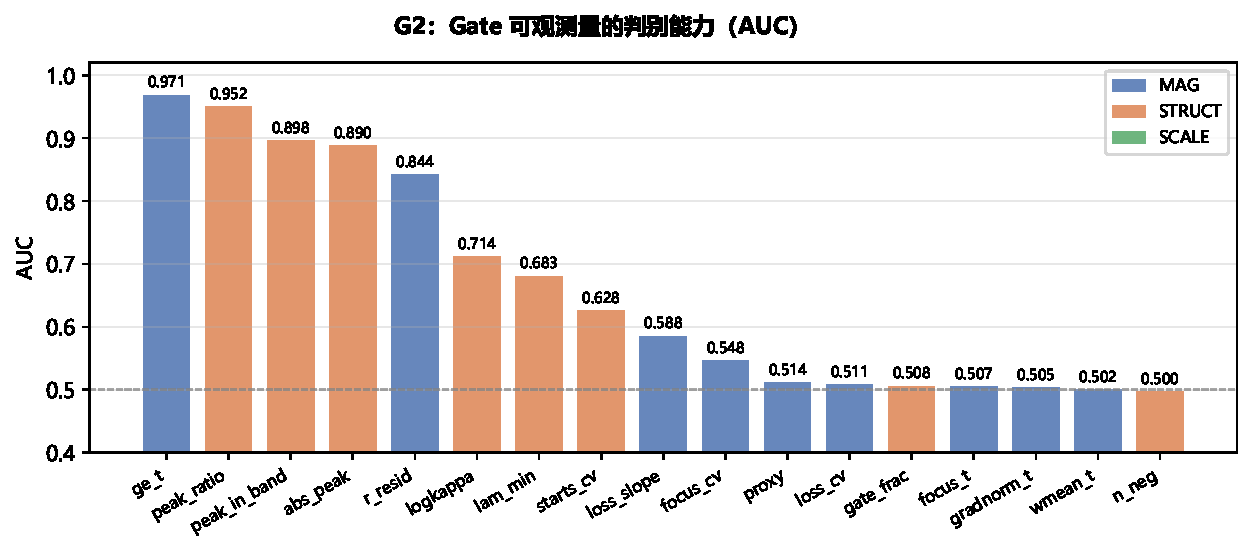
\includegraphics[width=0.92\textwidth]{fig_G2_auc_zh.pdf}
\caption{实验 6.1：各 Gate 可观测量的判别能力（AUC，$n=80$，proxy 标签口径）。梯度能量—对比度 $g_{et}$（MAG 组）AUC 最高（.971）；结构量组（STRUCT）内峰值比 $.95$、带内质量 $.90$、绝对峰值 $.89$ 较强，组内其余量 $.50$--$.71$；独立网格残差 RMS $r_{\rm resid}$（MAG 组）proxy 口径 $.84$，但 oracle 存在性口径仅 $.51$（验收/存在性分裂，见正文三层解读）；训练过程量（$7$ 个）AUC 中位 $.51$（近机会水平、不可判别），与 \S\ref{sec:gate} 的可识别性分析一致。}\label{fig:g2auc}
\end{figure}

\FloatBarrier

\section{跨方程验证}\label{sec:crosseqn}

本章在与 Burgers 相同的两阶段协议下，检验本文结论在其他方程类型上的适用性。核心问题是：\emph{空间加权的能力边界是否依赖 Burgers 的特定结构？}结论是：在光滑椭圆 Poisson 上增权无系统收益（退化验证），在内部奇性问题上表示层缺陷主导、空间加权无能为力（通道分离的可证伪预测）；并以一维时变 Burgers（实验 7.5）与二维线性对流—扩散（实验 7.7）两个轻量算例，检验上述边界在时间依赖与高维情形下的方向稳定性。

\subsection{Poisson 光滑退化对照（实验 7.1，$n=11$）}\label{sec:s2a}

\textbf{设置。}以解析解标定的椭圆型 Poisson 方程，解取单频与含 $3\pi$ 高频的多频两类；表示器取普通 MLP、匹配带宽 Fourier 特征（$\sigma=1$）与失配高带宽（$\sigma=15$）三种；权重取等权、有理增权与逆减权共 $7$ 个权重—对比度组合；每格 $n=11$ 个种子、固定 $3000$ 步，合计 $462$ 次训练。Poisson 解光滑、无激波，用于检验"无局域刚性时空间加权是否仍有收益"，配对检验用 Wilcoxon 符号秩。

\noindent\textbf{三结论（配对、$n=11$）}。
(i)~\emph{增权在光滑问题上无系统收益}：六组增权（$\beta=10$）—等权配对 Wilcoxon 对照中五组不显著，显著组仅（单频、$\sigma=1$）一组：中位 $L_2$ 反由 $1.41\times10^{-5}$ 升至 $1.11\times10^{-4}$（$p=.001$，逐种子配对变差倍数中位约 $5$；本节倍数一律取逐种子配对倍数的中位数，组间中位数仅描述各组水平）。这与机制 A 的预测一致（光滑端对比度可分条件不成立，增权无收益），但终态比较无法精确区分"梯度尺度调节"与"隐式谱对齐"两种机制归因，此处仅作方向一致性观察。
(ii)~\emph{逆减权的显著收益主要出现在"解含高频而表示带宽不足/频谱失配"时}：多频解配普通 MLP，中位 $L_2$ 由 $7.42\times10^{-3}$ 降至 $2.02\times10^{-4}$（$p=.001$，$11/11$ 全部改善，配对改善倍数中位约 $24$）；单频、$\sigma=1$ 时由 $1.41\times10^{-5}$ 降至 $4.05\times10^{-6}$（$p=.005$，$9/11$ 改善，配对倍数中位约 $3.3$；该组绝对误差本已处于 $10^{-5}$ 量级、接近误差地板，收益的实际意义有限）；失配高带宽（多频、$\sigma=15$）则由 $.108$ 升至 $.113$（$p=.001$，显著变差）。这与实验 4.3 相互印证：减权是梯度尺度调节器，其获益不要求局域刚性，而要求频谱失配导致的梯度尺度失衡。
(iii)~\emph{带宽—尺度匹配占主导}：失配高带宽比匹配带宽在光滑解上差 $40$--$1000$ 倍，三种加权均无法挽回；表示器带宽与解尺度的匹配先于、且强于空间加权。

\subsection{内部奇性闭环（实验 7.4/7.2/7.3）}\label{sec:s2singular}

\paragraph{统一框架：前向 ansatz、楔形误差与三类表示层干预。}前向表示统一写为
\[
u(x)=A(X(x))+B(X(x))\,N(\gamma(X(x))),
\]
其中 $A$ 为边界提升、$B$ 为满足齐次边界的湮灭因子、$X$ 为坐标映射、$\gamma$ 为输入特征/频率。对 $(-1,1)$ 上常用的 $B(x)=1-x^2$，网络部分对提升的偏差有逐点楔形界
\begin{equation}\label{eq:wedge}
|u(x)-A(x)|\le (1-x^2)\,\|N\|_\infty .
\end{equation}
楔形宽度在域内部为 $O(1)$（网络有充分修正力），在贴边 $x\to\pm1$ 退化为 $0$（无修正力，必须把边界层形状精确做进 $A$）。据此把表示层干预分为三类：\textbf{类型-I（边界编码）}（改 $A/B$）、\textbf{类型-II（坐标与测度）}（改 $X$）、\textbf{类型-III（内部拓扑缺陷）}（以内部缺陷的位置/拓扑调制 $\gamma$ 与初值）。空间加权与多起点\emph{不}改变 $A,B,X,\gamma$，故对 类型-I/II/III 的能力缺陷无能为力；这是层面分离在跨方程情形的可证伪预测。

\paragraph{实验 7.2 内部转向点层（类型-II 的正面几何迁移，全量 $n=11$）。}方程 $-\varepsilon u''-xu'=0$、$u(-1)=0,u(1)=1$，真解为误差函数、层在内部 $x=0$。$\varepsilon=.01/.001/10^{-4}$（等效 Burgers 粘度 $\nu_{\rm eq}=.058/.018/.0058$，按内部误差函数层与 Burgers 激波层同厚度的经验配对标定，属经验配对而非解析等价）。与 Burgers 相同的两阶段协议下，\textbf{[经验 $n=11$]} 三厚度 $K=4$ 选优均为 $11/11$ 进入可精修盆地，精修后全域相对 $L_2$ 中位为 $10^{-5}$ 量级。内部缺陷落在楔形最宽处，无需边界提升或拓扑种子即被精修。

\noindent\textbf{机制 A 在本算例上的条件性（与 Burgers 对照）。}冻结 Gate 点、同 $\theta$ 同 $r$ 仅改 $\beta\in\{1,3,8\}$，分区梯度能量比 $\eta=g_{\rm band}/g_{\rm smooth}$ 在 $7/11$ 个 Gate 点下降、$4/11$ 上升，平均 Spearman 秩相关约 $-0.32$（\textbf{对照 Burgers 四粘度全为 $+1$}）；原因是 $\beta$ 同时放大层带与光滑区梯度，而本线性层的 Gate 点层已基本成形、带内对比度分离（C-Sep）弱。配对精修（层区 $L_2$）：$\beta=3$ 对 $\beta=1$ 为 $8/11$ 更好、中位差 $-1.06\times10^{-5}$（Wilcoxon 双侧 $p=.41$，Holm 校正 $p=.56$），$\beta=8$ 为 $7/11$（$p=.28$，校正 $p=.56$），\emph{均不显著}；三档精修后 $L_2$ 均落在 $10^{-5}$--$10^{-4}$、殊途同归到由 Fourier 带宽决定的精度地板。这不是负结果，而是把机制 A 的适用边界钉死：增权的能量再分配收益严格依赖 Gate 点处带内对比度分离（C-Sep）与局域刚性；当问题线性、层心楔形最宽、无坏盆地而精度瓶颈在表示带宽时，$\beta$ 是中性的，与 Poisson 光滑退化（实验 7.1）的"增权无系统收益"从两侧夹出同一边界。

\paragraph{实验 7.3 Allen--Cahn 尖峰（类型-III：可表达$\ne$可到达，诊断级）。}方程 $-\varepsilon^2u''+u-u^3=0$ 存在同伦尖峰 $u^*(x)=\sqrt2\,\mathrm{sech}((x-x_0)/\varepsilon)$ 与零能基态 $u\equiv0$。取 $\varepsilon\in\{.01,.0044,.002\}$、普通 $K=4$ 网络、每档 $4$ 起点，\emph{无种子}时 $12/12$ 全部塌到 $u\equiv0$（残差可降至近零——$u\equiv0$ 本身即零残差解——而全域 $L_2\approx.999$），尽管 $u^*$ 在该网络类中可 $\varepsilon_0$-表达到远高于塌零率所需精度（纯监督拟合对照固定目标 $u^*$、$12$ 个独立种子，全域归一化 $L_2$ 中位 $6.2\times10^{-4}$、较塌零态的 $.999$ 低约三个数量级）——这是"可表达$\ne$可到达"的受控反例：缺陷不在表示容量，而在优化可达性（$\theta$ 初值的拓扑）。改用以 $x_0$ 为中心的拓扑种子（$\varepsilon=.0044$、每法 $4$ 起点）：精确 sech 种子 $4/4$ 命中；粗高斯种子在幅值 $.8/\sqrt2/2$、宽 $1.5\varepsilon$ 下均 $4/4$ 命中；唯当种子错位 $x_0=.15$（$\approx34\varepsilon$）时 $4/4$ 失败、峰湮灭。即拓扑种子\emph{位置必须对、形状/幅值/宽度可粗}，它以零阶表示的信息调制 $\theta$ 初值，发生在表示—优化接口。

\paragraph{实验 7.4 贴边对流—扩散层（类型-I：边界不可修正，诊断级）。}方程 $-\varepsilon u''+bu'=0$、层在边界 $x=1$，真解为指数、无激波。按层厚配对取等效 $\nu=.005$（$\varepsilon=.01$）：同厚度 Burgers 在 $K=8$ 的 $8$ 起点中 $3$ 个命中，而贴边层在 $\sigma=15/30$ 共 $16/16$ 零命中（$L_2=9.6$--$10.8$）。只改坐标映射 $X$（类型-II）：厚层 $\varepsilon=.1$ 拉伸 $4/4$ 成功，薄层 $\varepsilon=.01$ 拉伸 $8/8$ 失败——拉伸只重排测度，不补充贴边楔形所缺失的修正力。改边界提升 $A$（类型-I）：精确指数提升 $4/4$ 成功（全域 $1.6\times10^{-3}$--$3.3\times10^{-3}$），粗 logistic 提升 $8/8$ 失败。贴边层楔形退化为零，\emph{必须}把层形状精确做进 $A$，与内部缺陷的"粗几何可救"恰成对照。

\begin{figure}[ht]\centering
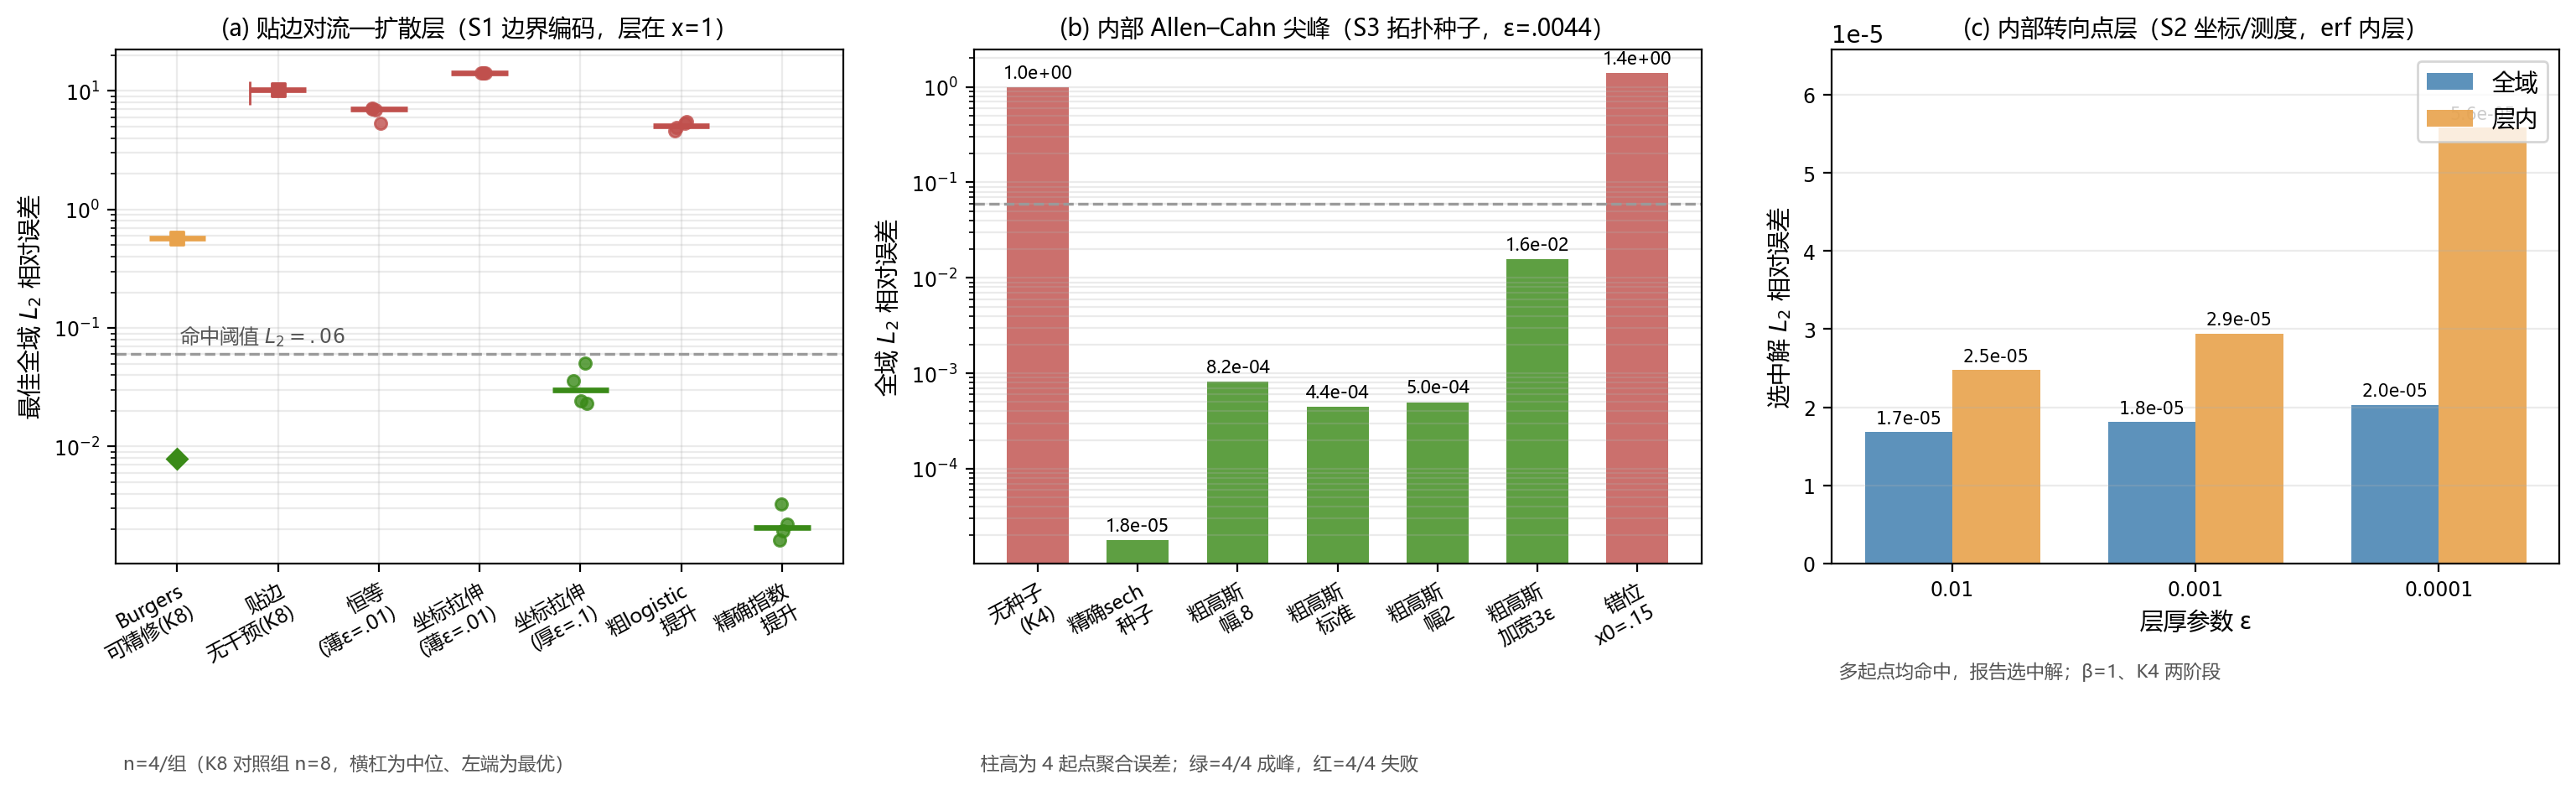
\includegraphics[width=0.99\linewidth]{fig_s2_singular_panel.png}
\caption{（定量；实验 7.2 全量 $n=11$，实验 7.4/7.3 为诊断级）(a) 贴边对流—扩散层：仅精确指数提升（类型-I）与厚层坐标拉伸（类型-II）成功，薄层拉伸、粗提升与无干预全部失败；(b) Allen--Cahn 内部尖峰：无种子 $12/12$ 塌零，居中拓扑种子 $4/4$ 成峰，错位 $34\varepsilon$ 即 $4/4$ 失败；(c) 内部转向点层三档厚度均精修到 $10^{-5}$ 量级。}\label{fig:s2panel}
\end{figure}

\subsection{一维时变 Burgers（实验 7.5，$n=11$）}\label{sec:d1}

\textbf{设置。}时变粘性 Burgers $u_t+uu_x=\nu u_{xx}$，$x\in[-1,1]$、$t\in[0,.99]$，$\nu=.01/\pi$，初值 $u(x,0)=-\sin(\pi x)$、边值 $u(\pm1,t)=0$（Raissi 标准算例，软边界），参考解取高分辨率谱/数值解。网络 $[2,50,50,50,50,1]$（$p=7851$），配点 $N=4300$（$4000$ PDE $+100$ BC $+200$ IC），固定步长 Adam 训练 $50000$ 步，权重取有理增权族 $w=(1+\beta t)/(1+t)$（$t=|r|/\mathrm{median}|r|$，与稳态实验 5.4/5.5 同族），强度 $\beta\in\{1,3,8,15\}$、每格 $n=11$ 颗等距种子（与稳态实验同一基础种子集 $S_0=\{0,5,\dots,50\}$）。好盆地阈值 $\tau=.06$ 按时空全域相对 $L_2$ 的自然间隙标定（四档排序值均在 $.056$--$.066$ 附近留有间隙，实验 6.2 式扫描见表注）。

\begin{table}[ht]\centering\small\renewcommand{\arraystretch}{1.2}
\begin{tabular}{cccc}
\toprule
$\beta$ & 中位时空全域 $L_2$ & $L_2$ 范围 & 好盆地数/$11$\\
\midrule
$1$  & $1.66\times10^{-2}$ & $[2.87\times10^{-3},\,.327]$ & $8$\\
$3$  & $1.53\times10^{-2}$ & $[6.56\times10^{-3},\,.150]$ & $9$\\
$8$  & $5.56\times10^{-2}$ & $[1.80\times10^{-2},\,.375]$ & $6$\\
$15$ & $5.35\times10^{-2}$ & $[2.90\times10^{-2},\,.105]$ & $8$\\
\bottomrule
\end{tabular}
\caption{（定量，实验 7.5，$n=11$）一维时变 Burgers 上不同固定强度的时空全域相对 $L_2$ 中位、范围与好盆地数（阈值 $\tau=.06$，位于四档排序值的自然间隙内）。$\beta=8/15$ 档好盆地数对阈值敏感：$\tau=.05/.06/.10$ 下 $\beta=8$ 为 $4/6/8$、$\beta=15$ 为 $5/8/10$；逐种子配对检验不依赖阈值取值。}\label{tab:d1beta}
\end{table}

\noindent\textbf{结论（表~\ref{tab:d1beta}）。}\textbf{[经验 $n=11$]}(i)~时变问题上仍存在好/坏盆地之分（四档均有失败种子，$\beta=1/3/8/15$ 的好盆地数为 $8/9/6/8$、失败者 $L_2$ 长尾至 $.1$--$.4$），但未观察到一维稳态刚性端那种稳定、对称的伪解双峰；盆地结构对时间推进与边界处理方式敏感。(ii)~配对 Wilcoxon signed-rank 检验显示各档间无显著差异（$\beta=1$ 对 $3/8/15$：$p=.41/.32/.37$，$n_{\rm eff}=11$）；逐种子最优归属为 $\beta=3$ 拿 $6/11$、$\beta=1$ 拿 $4/11$、$\beta=15$ 拿 $1/11$，高强度增权既能救活 $\beta=1$ 的灾难性失败（如 seed 30 由 $.327$ 降至 $.029$），也会在新种子上制造失败（$\beta=8$ 对 $\beta=1$ 的 $L_2$ 比值中位 $3.95$、最差近百倍），输赢相抵。即时变 Burgers 上有理增权\emph{近中性}：机制 A 照常触发（(iii)），但不转化为系统收益，也不制造系统失败。同一方程在空间线性族下为"增权有害"（$\beta=8/15$ 零好盆地）、早期另一套 $\nu$/种子口径的空间线性族扫描曾得"增权有益"——结论随权重族反转本身即说明时变盆地结构对权重族与协议敏感。本节与实验 7.1/7.2/7.7 共同确认：空间加权在时变与光滑/线性问题上无系统收益。(iii)~\emph{机制~A 跨方程旁证}：在 Gate 点冻结、同 $\theta$ 同 $r$ 仅把 $\beta=1$ 换成 $8$，加权前后梯度方向余弦中位 $.9999$（范围 $.999$--$1.000$，方向几乎不变）、总梯度范数比中位 $7.75$（$7.15$--$7.84$，$\approx\beta$，整体放大尺度）、中心区/边界区梯度行范数比由 $2.90$ 抬到 $4.20$；即增权主要做梯度尺度的空间再分配、几乎不改变梯度方向，与稳态机制~A 的刻画一致。

\par\smallskip\noindent\textbf{诊断级观察（人为坏盆地，实验 7.6，$n=11$，Adam $20000$ 步）。}以零初值等手段把初值人为置于坏盆地（终态 $L_2\approx2.5$、$0/11$ 进入好盆地）后：减权 $\beta=1/3,\,1/8$（空间线性族）中位 $L_2=2.75/2.86$（\emph{更差}），梯度裁剪（阈值 $.01/.1$）与对照逐位相同（$2.57$，未改变终态），轻微增权 $\beta=3,\,8$（$2.44$）仍留在坏盆地。即一旦初值落入坏盆地，空间减权与显式梯度裁剪均无法将其救出，与稳态实验 5.3"减权不是盆地逃逸机制"相互印证，且时变上裁剪同样无效。该 setup 为人为构造的诊断实验、非自然训练分布，系统的时变配对实验留待后续。

\begin{figure}[ht]\centering
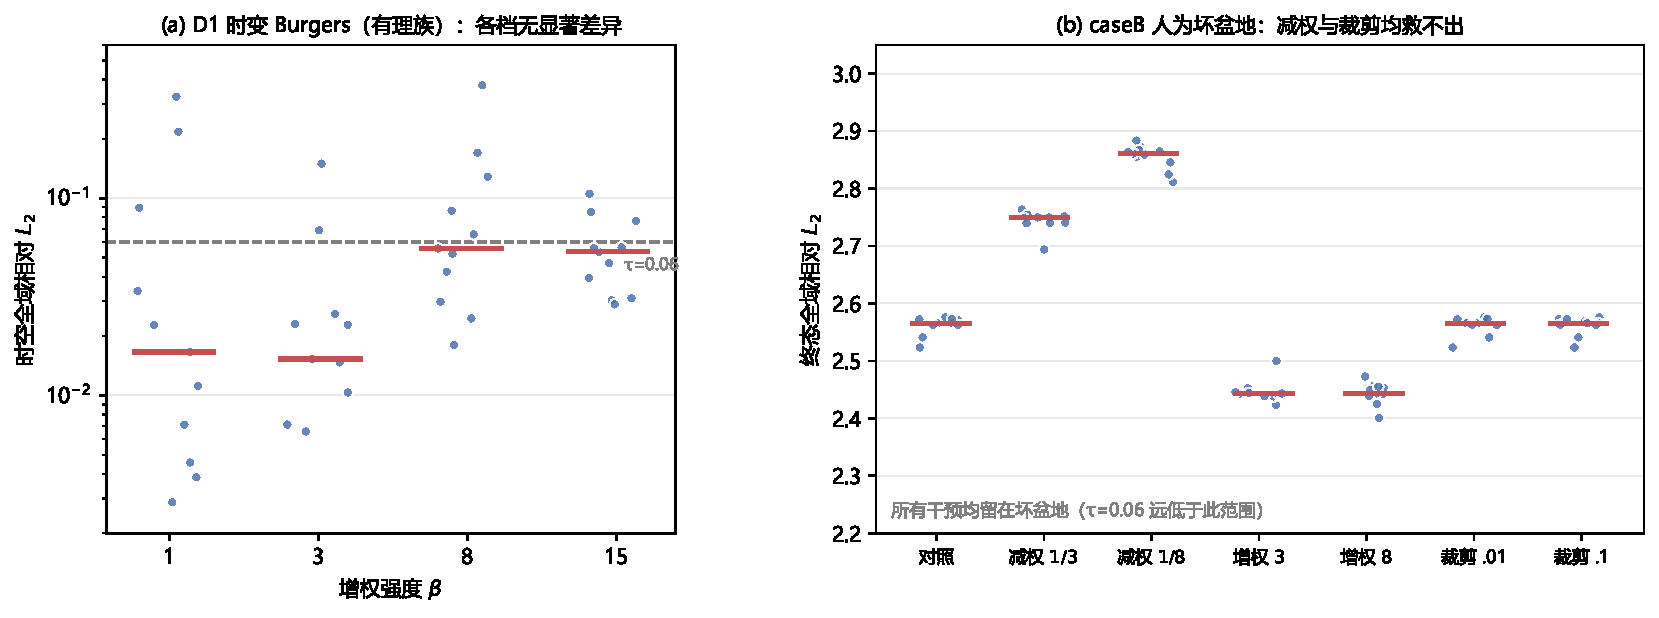
\includegraphics[width=0.98\textwidth]{fig_d1_caseb_zh.pdf}
\caption{(a)~实验 7.5（一维时变 Burgers，有理族，$n=11$）四档固定强度的逐种子时空全域相对 $L_2$（对数轴），虚线为好盆地阈值 $\tau=.06$：各档均有失败种子，配对检验无显著差异（$p=.41/.32/.37$），有理增权近中性。(b)~实验 7.6 人为坏盆地诊断（空间线性族，$n=11$，Adam $20000$ 步，诊断级）：减权 $\beta=1/3,\,1/8$、梯度裁剪（阈值 $.01/.1$）与轻微增权 $\beta=3,\,8$ 相对对照的终态 $L_2$ 分布；各干预均无法逃逸坏盆地（裁剪与对照逐位相同）。}\label{fig:d1caseb}
\end{figure}

\subsection{二维线性对流—扩散（实验 7.7，$n=11$）}\label{sec:c45}

\textbf{设置。}二维线性对流—扩散方程（周期边界、含初值），解光滑、无内部激波或薄边界层；网络输入维 $d_{\rm in}=3+4K$（$K=32$ Fourier 特征），$p=14301$，配点 $N=4200$（$4000$ PDE $+200$ IC），固定步长 Adam。先以等权 $\beta=1$ 作 baseline，再扫 $\beta\in\{1,3,8\}$，每格 $n=11$ 颗等距种子。

\begin{table}[ht]\centering\small\renewcommand{\arraystretch}{1.2}
\begin{tabular}{cccc}
\toprule
$\beta$ & 中位 $L_2$ & $L_2$ 范围 & 最大 $L_2$\\
\midrule
$1$ & $5.06\times10^{-2}$ & $[.0461,\,.0628]$ & $.0628$\\
$3$ & $5.03\times10^{-2}$ & $[.0418,\,.0582]$ & $.0582$\\
$8$ & $4.85\times10^{-2}$ & $[.0414,\,.0583]$ & $.0583$\\
\bottomrule
\end{tabular}
\caption{（定量，实验 7.7，$n=11$）二维线性对流—扩散上不同固定强度的时空全域相对 $L_2$ 中位、范围与最大值；全部 $33$ 个 run 的 $L_2\le.0628$、无失败种子，故本算例不设好盆地阈值。}\label{tab:c45}
\end{table}

\noindent\textbf{结论（表~\ref{tab:c45}，单一配置、方向级示意）。}\textbf{[经验 $n=11$]}全部 $33$ 个 run 的 $L_2\le.0628$、无失败种子、未观察到伪解双峰；$\beta=1\to8$ 中位 $L_2$ 仅 $.0506\to.0485$（约 $4\%$ 的同量级波动），空间加权近中性。它与 Poisson 光滑退化（实验 7.1）从一维、二维两侧共同确认：在无局域刚性对比度（C-Sep 不成立）、亦无坏盆地的光滑/线性问题上，空间加权既无系统收益、也不制造失败。

\begin{figure}[ht]\centering
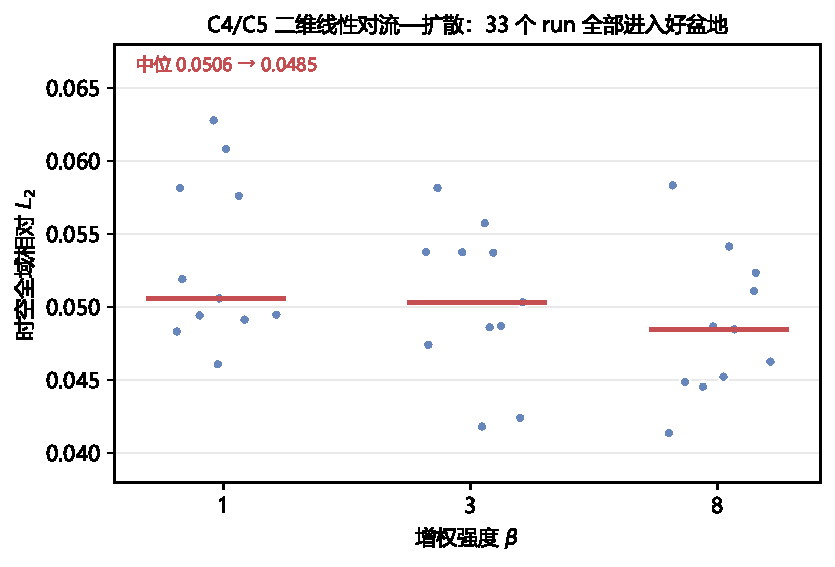
\includegraphics[width=0.85\textwidth]{fig_c45_advdiff_zh.pdf}
\caption{（定量，实验 7.7，$n=11$）二维线性对流—扩散上 $\beta=1/3/8$ 三档共 $33$ 个 run 的逐种子时空全域相对 $L_2$（虚线 $\tau=.06$ 为实验 7.5 的好盆地阈值，仅作参照）：全部 $33$ 个 run 的 $L_2\le.0628$、无失败种子，三档分布高度重叠，空间加权近中性。}\label{fig:c45}
\end{figure}

\noindent\textbf{跨方程验证小结。}上述原型（图~\ref{fig:s2panel}）在稳态、一维下闭环了"表示层三分类"的判别力：内部缺陷（实验 7.2）落在楔形最宽处、空间加权中性；内部拓扑缺陷（实验 7.3）需拓扑种子、空间加权无能为力；贴边层（实验 7.4）需精确边界提升、空间加权无能为力。三者共同验证了层面分离的可证伪预测：空间加权不改变表示层 $A,B,X,\gamma$，故对表示层缺陷无能为力。在此之外，一维时变 Burgers（实验 7.5，\S\ref{sec:d1}）上高强度固定增权同样不带来系统收益、减权与裁剪均无法救出人为坏盆地，且机制~A 的"增权放尺度、几乎不改方向"在时变上复现；二维线性对流—扩散（实验 7.7，\S\ref{sec:c45}）上 $33$ 个 run 全部无失败种子（$L_2\le.0628$）、加权近中性。水锤、浅水等双曲/方程组情形与二维刚性算例，按同一受控协议留待后续工作。

\FloatBarrier

\section{适用范围与结论}\label{sec:conclusion}

\subsection{方程无关内核与方程相关常数}\label{sec:scope}

本文的确定性结论分为两层。\emph{方程无关内核}（在各命题自身假设下不依赖 Burgers 结构、适用于一般光滑 PDE 与网络架构）包括：零残差集对正权不变（命题~\ref{prop:zero}）；残差—误差桥的线性部分（命题~\ref{prop:bridge}）；局部对角权的谱能力边界（定理~\ref{thm:local-cap}，仅用同时对角化、相关矩阵恒等式与 van der Sluis 定理）；等相关类在对角缩放下条件数已最优（定理~\ref{thm:equicorr}）；固定单投影标量的可识别性下界与四点反例（命题~\ref{prop:bayes}）；增/减权的一阶方向判据（命题~\ref{prop:align}）。这些结论的\emph{陈述}不依赖具体方程，但其中涉及的\emph{常数}（如稳定性常数 $C_{\rm loc}$、条件数 $\kappa(K_r)$、有效秩 $PR$、对比度分离程度 C-Sep）是方程与参数相关的。

\emph{方程相关的经验结论}（在一维稳态 Burgers 上验证、需在其他方程上重新检验）包括：机制 A 的 $\eta_{gate}$ 单调性（实验 5.1/5.2）；未观察到减权能提高盆地进入概率（实验 5.3，$n=80$）；可精修盆地内 $\beta^*$ 的 regime（实验 5.4/5.5/5.6，$n=11$）；训练过程 Hessian 条件数的动态记录（实验 4.3）；无真解判别中结构量 $g_et$ 的可行性（实验 6.1，$n=80$）。这些结论的\emph{定性方向}（未观察到空间加权能选择盆地、增权收益依赖局域刚性、减权是梯度尺度调节器、其收益依赖尺度是否为瓶颈）在 Poisson（实验 7.1）和内部奇性（实验 7.4/7.2/7.3）上得到了跨方程验证，但\emph{定量常数}（如 $\beta^*$ 的具体值、增益的倍数）是方程相关的。

\subsection{向新权重族与新方程迁移的判据}\label{sec:migration}

本文结论向新权重族迁移的适用条件如下：
\begin{enumerate}[label=(\arabic*),leftmargin=2em,itemsep=1pt]
\item \textbf{正对角、逐点（局部）乘性}：满足时，定理~\ref{thm:local-cap} 的谱能力边界直接适用；引入非对角（卷积/算子预条件）或可训练权重 $\W(\theta)$ 则超出本文框架。
\item \textbf{原则 I--II（仅梯度算法类）}：权重由含 $\W$ 的量触发（如按加权损失 $L_\W$ 自适应调整）时违反原则 II，不在本文覆盖内。
\item \textbf{权重冻结或外生缓变}：每步重算 $w(t_i(\theta))$ 时 $\nabla_\theta\W\ne0$，加权梯度不再是 $J^\top\W r$，本文的线性化框架不直接适用。
\end{enumerate}

迁移到新方程时，以下性质决定本文定性结论是否预期保持：
\begin{enumerate}[label=(\arabic*),leftmargin=2em,itemsep=1pt]
\item \textbf{局域刚性对比度（C-Sep）}：不存在时（如光滑 Poisson），机制 A 的增权收益预期消失。
\item \textbf{好/伪解双稳盆地结构}：不存在时（如内部转向点层实验 7.2），盆地选择问题不出现，空间加权的作用窗口缩小。
\item \textbf{表示器—尺度匹配}：表示带宽与解尺度失配时（如固定高带宽在光滑端），表示层缺陷主导、空间加权无法挽回。
\end{enumerate}

\subsection{Jacobi 均衡与梯度范数加权的关系}\label{sec:jacobi-gap}

实验 4.2 的三元组显示，实践者起点（均匀权 $\kappa(K_r)$）与无约束上界（$\kappa^*_{\rm diag}$）之间的差距，线性 gap 口径下 $>85\%$ 可由 Jacobi 均衡 $w_i\propto(K_r)_{ii}^{-1/2}$ 这一简单局部对角权填补。本文的谱扫描覆盖 rational 族（表~\ref{tab:f1d-triplet}）：族内最优恒为 $\beta=1$（均匀权），与 Jacobi 存在数量级差距；其余对比度族未做谱扫描，本文不对其谱性质作断言。

Jacobi 均衡在 PINN 语境下恰是\emph{梯度范数加权}：$(K_r)_{ii}=\|J_i\|^2$ 是第 $i$ 个配点残差梯度的行范数平方，故 $w_i\propto 1/\|J_i\|$。这与 Wang、Teng 与 Perdikaris\cite{WangTeng2020} 提出的学习率退火（按梯度范数比调整各损失项学习率）属同一族方法——实验 4.2 为退火的有效性提供了\emph{二阶谱层面的机理解释}：梯度范数归一化恰好是 Jacobi 均衡，能把条件数从均匀权水平拉到相关阵 $R(K_r)$ 的水平，而 rational 族连这一步都达不到（族内最优即均匀权，见上）。

本文\emph{未}在训练实验中测试动态 Jacobi 加权（每步重算 $w_i\propto 1/\|J_i(\theta)\|$），原因有二：(1) 动态 Jacobi 属在线重算 $\W(\theta)$，违反原则 II（$\nabla_\theta\W\ne0$），超出本文冻结/外生缓变口径的理论覆盖范围；(2) 每步行范数计算成本为 $O(Np)$，与对比度权的 $O(N)$ 不同。静态 Jacobi（在 Gate 点冻结一次）属外生缓变口径、理论可覆盖，是低成本的未来工作方向；动态 Jacobi 的修正梯度分析（$g=J^\top\diag(m_{ad})r$，见引理~\ref{lem:linrec}(ii)）与在线加权的通道 $\theta$ 效应，列为后续工作（\S\ref{sec:future}）。

\subsection{经验观察：二阶谱不决定盆地，表示层才是盆地的主导因素}\label{sec:S-observation}

本文全部实验一致指向一个超出"加权能力边界"的观察：在固定网络表示（架构、边界编码、坐标映射、Fourier 特征带宽）的条件下，空间加权不改变损失景观的吸引域拓扑，只改变梯度的尺度分布；盆地的存在性与可达性由表示层的表达能力和编码几何决定。支持证据如下：

\begin{enumerate}[label=(\arabic*),leftmargin=2em,itemsep=1pt]
\item \textbf{边界编码（类型-I）改变吸引域}：硬边界 ansatz（$u=(1-x^2)v$）与软边界（损失项惩罚）是两类不同的零阶表示；硬边界幅值编码的错误会把端点误差钉死（见复现细节 B.5 审计），时变算例实验 7.5 则在软边界设置下训练。本文观察到大粘性端两类编码下训练行为存在质变，但\emph{未做}同一配置下严格的软/硬配对对照，故此处仅作方向性证据，系统比较留待后续。
\item \textbf{坐标与测度（类型-II）与边界层的几何冲突}：椭圆方程的边界层算例实验 7.4 中，硬边界编码与边界层的几何结构冲突，必须依赖真解结构（坐标拉伸）才能缓解；纯空间加权无法解决。内部奇异点算例实验 7.2/7.3 显示 $u\equiv0$ 为稳定局部极小、初始化敏感性主导，"可表示 $\neq$ 可达"。
\item \textbf{表示带宽与解尺度的匹配（类型-III，特征/拓扑侧）}：Fourier 特征带宽 $\sigma$ 与解的尺度失配时（固定高带宽在光滑端），表示层缺陷主导、空间加权无法挽回（实验 5.6 退化扫描）；大粘性退化的根因是带宽不足而非权重不当。
\item \textbf{二阶层面干预未提升、减权族降低盆地进入}：实验 5.3（$n=80$）显示无加权族提升进入率，uniform 命中率 $.613$ 最高；减权族 down\_lin 经 Holm 校正后\emph{显著降低}进入率（$.388$，校正 $p=.006$），down\_inv/rational 亦低于 uniform。即空间加权（至少减权族）实测改变盆地归属概率、方向为负；实验 5.9 显示固定步长 L-BFGS 下四族终态差异不显著。
\end{enumerate}

该观察的推论是：文献中大量"加权改善训练"的说法，其收益可能实际来自伴随的表示层变化（如自适应采样改变了测度、硬边界编码改变了表示），而非权重本身。严格分离零阶/一阶/二阶三个层面的干预，是理解 PINN 训练机制的必要前提。本观察为经验归纳（\textbf{[经验]}），非严格定理；其严格化与系统分类列为后续工作（\S\ref{sec:future} 第 3 项）。

\subsection{未来工作与开放问题}\label{sec:future}

本文划定了空间静态加权在上述分层下的能力边界。以下方向超出本文范围，列为未来工作：

\begin{enumerate}[label=(\arabic*),leftmargin=2em,itemsep=1pt]
\item \textbf{通道 $\theta$ 的构造性训练理论}：盆地内一阶方向判据与"本盆地驻点/真解"两个参照系的对齐；盆地内最优强度 $\beta^*$ 的条件存在性与误差的多项分解；减权转增权的安全切换条件；含进入概率 $p_{entry}(1-\delta)$ 的两阶段条件误差界。
\item \textbf{多层面协同与冲突}：在上述分层下设计新算法，研究零阶（表示）、二阶（谱）、一阶（优化动力学）的干预是相辅相成还是互相掐架；非局部/卷积权重、算子预条件、在线自适应权重的严格分析。
\item \textbf{表示层的分类性质}：基于本文实验 7.4/7.2/7.3 的发现，系统研究边界编码、坐标与测度、内部拓扑缺陷三类表示层干预的能力边界与统一框架；硬边界处理方法对表示层的影响。
\item \textbf{跨方程与时变/高维验证}：本文已在一维时变 Burgers（实验 7.5）与二维线性对流—扩散（实验 7.7）上做轻量跨方程验证；水锤、浅水等双曲/方程组情形、二维刚性 Burgers 与系统的时变配对实验仍待完成。真解优先取开源（BSD/MIT 许可）高分辨率参考解。
\item \textbf{Gate 方法学的深化}：Gate-A 三条触发规则的效能标定（三条同时成立时多大概率进入可精修盆地、能否去掉某条、最弱可检验替代）；结构量的最小充分集及其紧致性；跨粘度、跨方程部署的充分条件。
\end{enumerate}

\noindent\textbf{总结。}本文从零阶/一阶/二阶三个层面严格刻画了空间静态对角加权的能力边界：在二阶层面上，局部对角权不能改变相关矩阵 $R(K_r)$、在等相关类上不改善条件数、近奇异时最优条件数仍无界（定理~\ref{thm:local-cap}，静态实验 4.2 + 动态实验 4.3 双重验证）；在一阶层面上，未观察到加权能改善盆地进入（实验 5.3，$n=80$ 配对拒绝减权逃逸假说，不作全称否定），其有益效应限于已进入可精修盆地内的收敛速度调节（增权收益严格依赖局域刚性对比度，机制 A，实验 5.4/5.5/5.6，$n=11$）与梯度尺度调节（减权的真实定位，实验 4.3；频谱失配下的终态收益见第~\ref{sec:crosseqn}~章）；在方法学上，残差/损失自评估类固定单投影标量不能可靠判别盆地好坏（命题~\ref{prop:bayes}，实验 6.1 验证结构量 $g_et$ 的可行性）；在跨方程验证上，光滑 Poisson 上增权无系统收益（实验 7.1），内部奇性问题上表示层缺陷主导、空间加权无能为力（实验 7.4/7.2/7.3）；一维时变 Burgers（实验 7.5）上高强度增权无系统收益、减权与裁剪救不出人为坏盆地，二维线性对流—扩散（实验 7.7）上加权近中性、无失败种子（$L_2\le.0628$），能力边界在时间依赖与高维的光滑/线性情形方向不变。本文的贡献是能力边界的刻画与受控证伪，而非新算法的提出；构造性训练理论与多通道协同算法留待后续工作。

\FloatBarrier

\section*{致谢与 AI 使用声明}
本文准备过程中使用了 AI 助手豆包（字节跳动）与 Kimi（月之暗面）辅助文献核对、语言润色与代码/数据核验。作者对上述工具的输出进行了逐条审阅与修改，对本文内容承担全部责任。

\section*{数据可用性声明}
本文全部实验代码、处理后数据与可复现分析脚本开源于 GitHub：\url{https://github.com/wm2243/pinn-capability-boundary}（代码采用 MIT 许可，文本与图采用 CC-BY-4.0）；原始运行数据存档于 Zenodo（DOI：10.5281/zenodo.23168250）。

\begin{thebibliography}{99}\small
\bibitem{Raissi2019} M.~Raissi, P.~Perdikaris, G.~E.~Karniadakis. Physics-informed neural networks: A deep learning framework for solving forward and inverse problems involving nonlinear partial differential equations. \emph{Journal of Computational Physics}, 378:686--707, 2019.
\bibitem{Karniadakis2021} G.~E.~Karniadakis, I.~G.~Kevrekidis, L.~Lu, P.~Perdikaris, S.~Wang, L.~Yang. Physics-informed machine learning. \emph{Nature Reviews Physics}, 3:422--440, 2021.
\bibitem{Cuomo2022} S.~Cuomo, V.~S.~Di~Cola, F.~Giampaolo, G.~Rozza, M.~Raissi, F.~Piccialli. Scientific machine learning through physics-informed neural networks: Where we are and what's next. \emph{Journal of Scientific Computing}, 92:88, 2022.
\bibitem{Shin2020} Y.~Shin, J.~Darbon, G.~E.~Karniadakis. On the convergence of physics informed neural networks for linear second-order elliptic and parabolic type PDEs. \emph{Communications in Computational Physics}, 28(5):2042--2074, 2020.
\bibitem{MishraMolinaro2020} S.~Mishra, R.~Molinaro. Estimates on the generalization error of physics-informed neural networks for approximating PDEs. arXiv:2006.16144, 2020.
\bibitem{DeRyckMishra2022} T.~De~Ryck, S.~Mishra. Error analysis for physics-informed neural networks approximating Kolmogorov PDEs. arXiv:2106.14473, 2021.
\bibitem{DeRyckMishra2024} T.~De~Ryck, S.~Mishra. Numerical analysis of physics-informed neural networks and related models in physics-informed machine learning. \emph{Acta Numerica}, 33:633--713, 2024.
\bibitem{vanDerMeer2020} R.~van~der~Meer, C.~Oosterlee, A.~Borovykh. Optimally weighted loss functions for solving PDEs with neural networks. \emph{Journal of Computational and Applied Mathematics}, 405:113887, 2022.
\bibitem{Maddu2021} S.~Maddu, D.~Sturm, C.~L.~M\"uller, I.~F.~Sbalzarini. Inverse-Dirichlet weighting enables reliable training of physics informed neural networks. \emph{Machine Learning: Science and Technology}, 3(1):015026, 2022; arXiv:2107.00940.
\bibitem{WangTeng2020} S.~Wang, Y.~Teng, P.~Perdikaris. Understanding and mitigating gradient flow pathologies in physics-informed neural networks. \emph{SIAM Journal on Scientific Computing}, 43(5):A3055--A3081, 2021.
\bibitem{Wang2020NTK} S.~Wang, X.~Yu, P.~Perdikaris. When and why PINNs fail to train: A neural tangent kernel perspective. \emph{Journal of Computational Physics}, 449:110768, 2022.
\bibitem{Jacot2018} A.~Jacot, F.~Gabriel, C.~Hongler. Neural tangent kernel: Convergence and generalization in neural networks. \emph{Advances in Neural Information Processing Systems (NeurIPS)}, 2018.
\bibitem{Liu2022down} L.~Liu, S.~Liu, H.~Xie, F.~Xiong, T.~Yu, M.~Xiao, L.~Liu, H.~Yong. Discontinuity computing using physics-informed neural networks. \emph{Journal of Scientific Computing}, 98:22, 2024.
\bibitem{LessEmphasis2022} Y.~Wang, C.~Xu, M.~Yang, J.~Zhang. Less emphasis on hard regions: Curriculum learning of physics-informed neural networks for singularly perturbed convection-diffusion-reaction problems. arXiv:2210.12685, 2022.
\bibitem{Wang2022causal} S.~Wang, S.~Sankaran, P.~Perdikaris. Respecting causality for training physics-informed neural networks. \emph{Computer Methods in Applied Mechanics and Engineering}, 421:116813, 2024.
\bibitem{ConFIG2025} Q.~Liu, M.~Chu, N.~Thuerey. ConFIG: Towards conflict-free training of physics-informed neural networks. \emph{International Conference on Learning Representations (ICLR)}, 2025.
\bibitem{Krishnapriyan2021} A.~Krishnapriyan, A.~Gholami, S.~Zhe, R.~Kirby, M.~W.~Mahoney. Characterizing possible failure modes in physics-informed neural networks. \emph{NeurIPS}, 2021.
\bibitem{Bengio2009} Y.~Bengio, J.~Louradour, R.~Collobert, J.~Weston. Curriculum learning. \emph{ICML}, 2009.
\bibitem{Hazan2016} E.~Hazan, K.~Levy, S.~Shalev-Shwartz. On graduated optimization for stochastic non-convex problems. \emph{ICML}, 2016.
\bibitem{Mobahi2015} H.~Mobahi, J.~W.~Fisher~III. A theoretical analysis of optimization by Gaussian continuation. \emph{AAAI}, 1205--1211, 2015.
\bibitem{Lee2016} J.~D.~Lee, M.~Simchowitz, M.~I.~Jordan, B.~Recht. Gradient descent only converges to minimizers. \emph{Conference on Learning Theory (COLT)}, 2016.
\bibitem{LiuZhuBelkin2021} C.~Liu, L.~Zhu, M.~Belkin. Loss landscapes and optimization in over-parameterized non-linear systems and neural networks. \emph{Applied and Computational Harmonic Analysis}, 59:85--116, 2022.
\bibitem{ZhouGeJin2021} M.~Zhou, R.~Ge, C.~Jin. A local convergence theory for mildly over-parameterized two-layer neural network. arXiv:2102.02410, 2021.
\bibitem{AttouchBolte} H.~Attouch, J.~Bolte, B.~F.~Svaiter. Convergence of descent methods for semi-algebraic and tame problems: Proximal algorithms, iterative methods and the {\L}ojasiewicz inequality. \emph{Mathematical Programming}, 137:91--124, 2013.
\bibitem{vanderSluis1969} A.~van~der~Sluis. Condition numbers and equilibration of matrices. \emph{Numerische Mathematik}, \textbf{14}(1):14--23, 1969.
\bibitem{Osborne1960} E.~E. Osborne. On pre-conditioning of matrices. \emph{Journal of the ACM}, 7(4):338--345, 1960.
\bibitem{RoosStynesTobiska1996} H.-G. Roos, M. Stynes, L. Tobiska. \emph{Numerical Methods for Singularly Perturbed Differential Equations: Convection--Diffusion and Flow Problems}. Springer, 1996.
\bibitem{Bhatia} R.~Bhatia. \emph{Matrix Analysis}. Springer, 1997.
\bibitem{HornJohnson} R.~A.~Horn, C.~R.~Johnson. \emph{Matrix Analysis} (2nd ed.). Cambridge University Press, 2013.
\bibitem{Strassen1965} V.~Strassen. The existence of probability measures with given marginals. \emph{Annals of Mathematical Statistics}, 36(2):423--439, 1965.
\bibitem{McClenny2020} L.~D.~McClenny, U.~M.~Braga-Neto. Self-adaptive physics-informed neural networks. \emph{Journal of Computational Physics}, 474:111722, 2023.
\bibitem{Nabian2021} M.~A.~Nabian, R.~J.~Gladstone, H.~Meidani. Efficient training of physics-informed neural networks via importance sampling. \emph{Computer-Aided Civil and Infrastructure Engineering}, 36(8):962--977, 2021.
\bibitem{Wu2022} C.~Wu, M.~Zhu, Q.~Tan, Y.~Kartha, L.~Lu. A comprehensive study of non-adaptive and residual-based adaptive sampling for physics-informed neural networks. \emph{Computer Methods in Applied Mechanics and Engineering}, 403:115671, 2023.
\bibitem{TangDAS2023} K.~Tang, X.~Wan, C.~Yang. DAS-PINNs: A deep adaptive sampling method for solving high-dimensional partial differential equations. \emph{Journal of Computational Physics}, 476:111868, 2023.
\bibitem{Rahaman2019} N.~Rahaman, A.~Baratin, D.~Arpit, et~al. On the spectral bias of neural networks. \emph{ICML}, 2019.
\bibitem{Tancik2020} M.~Tancik, P.~P.~Srinivasan, B.~Mildenhall, et~al. Fourier features let networks learn high frequency functions in low dimensional domains. \emph{NeurIPS}, 2020.
\bibitem{deRyckOp2024} T.~De~Ryck, F.~Bonnet, S.~Mishra, E.~de~B\'ezenac. An operator preconditioning perspective on training in physics-informed machine learning. \emph{International Conference on Learning Representations (ICLR)}, 2024; arXiv:2310.05801.
\bibitem{PCPINN2024} S.~Liu, C.~Su, J.~Yao, Z.~Hao, H.~Su, Y.~Wu, J.~Zhu. Preconditioning for physics-informed neural networks. \emph{Proceedings of the 41st International Conference on Machine Learning (ICML)}, 2024; arXiv:2402.00531.
\bibitem{SiYan2025} C.~Si, M.~Yan. Convolution-weighting method for the physics-informed neural network: A primal-dual optimization perspective. arXiv:2506.19805, 2025.
\bibitem{Rathore2024} P.~Rathore, W.~Lei, Z.~Frangella, L.~Lu, M.~Udell. Challenges in training PINNs: A loss landscape perspective. \emph{International Conference on Machine Learning (ICML)}, 2024; arXiv:2402.01868.
\bibitem{Bonfanti2024} A.~Bonfanti, G.~Bruno, C.~Cipriani. The challenges of the nonlinear regime for physics-informed neural networks. \emph{Advances in Neural Information Processing Systems (NeurIPS)}, 2024.
\bibitem{WangPseudo2026} S.~Wang, S.~Koohy, Y.~Lu, P.~Perdikaris. When PINNs go wrong: Pseudo-time stepping against spurious solutions. arXiv:2604.23528, 2026.
\bibitem{Rohrhofer2022} F.~M.~Rohrhofer, S.~Posch, C.~G\"o{\ss}nitzer, B.~C.~Geiger. On the role of fixed points of dynamical systems in training physics-informed neural networks. arXiv:2203.13648, 2022.
\bibitem{Musah2026} R.~Musah. Inverted model selection in physics-informed neural networks: when a lower residual selects a worse solution. arXiv:2608.21683, 2026.
\bibitem{Zou2025ensemble} Z.~Zou, Z.~Wang, G.~E.~Karniadakis. Learning and discovering multiple solutions using physics-informed neural networks with random initialization and deep ensemble. arXiv:2503.06320, 2025.
\bibitem{Daw2022Evo} A.~Daw, J.~Bu, S.~Wang, P.~Perdikaris, A.~Karpatne. Mitigating propagation failures in physics-informed neural networks using retain-resample-release (R3) sampling. \emph{International Conference on Machine Learning (ICML)}, 2023; arXiv:2207.02338.
\bibitem{Sukumar2022distance} N.~Sukumar, A.~Srivastava. Exact imposition of boundary conditions with distance functions in physics-informed deep neural networks. \emph{Computer Methods in Applied Mechanics and Engineering}, 389:114333, 2022.
\bibitem{GuanElman2024} J.~Guan, H.~Elman. Transformed physics-informed neural networks for the convection-diffusion equation. arXiv:2409.07671, 2024.
\bibitem{Leng2022hyperplane} K.~Leng, J.~Thiyagalingam. On the compatibility between a neural network and a partial differential equation for physics-informed learning. arXiv:2212.00270, 2022.
\bibitem{Akram2025} W.~Akram, S.~Gautam, D.~Verma, M.~T.~Mohan. Error estimates for viscous Burgers' equation using deep learning. arXiv:2502.19392, 2025.
\bibitem{ForsytheStraus1955} G.~E.~Forsythe, E.~G.~Straus. On best conditioned matrices. \emph{Proceedings of the American Mathematical Society}, 6(3):340--345, 1955.
\bibitem{Shapiro1982} A.~Shapiro. Optimally scaled matrices, necessary and sufficient conditions. \emph{Numerische Mathematik}, 39:239--245, 1982.
\bibitem{LivneGolub2004} O.~E.~Livne, G.~H.~Golub. Scaling by binormalization. \emph{Numerical Algorithms}, 35(1):97--120, 2004.
\bibitem{Qu2025ODP} Z.~Qu, W.~Gao, O.~Hinder, Y.~Ye, Z.~Zhou. Optimal diagonal preconditioning. \emph{Operations Research}, 73(3):1479--1495, 2025.
\bibitem{Jambulapati2020} A.~Jambulapati, J.~Li, C.~Musco, A.~Sidford, K.~Tian. Fast and near-optimal diagonal preconditioning. arXiv:2008.01722, 2020.
\bibitem{Gao2024SODP} W.~Gao, Z.~Qu, M.~Udell, Y.~Ye. Scalable approximate optimal diagonal preconditioning. \emph{Computational Optimization and Applications}, 94(2):439--473, 2026; arXiv:2312.15594.
\bibitem{FP64Xu2025} C.~Xu, D.~Liu, A.~Nassereldine, J.~Xiong. FP64 is all you need: Rethinking failure modes in physics-informed neural networks. arXiv:2505.10949, 2025.
\bibitem{KroneckerPINN2026} Y.~Park, J.~Kim, J.~Hong. Coupling-robust accuracy in multiphysics physics-informed neural networks via Kronecker-preconditioned optimization. arXiv:2605.23391, 2026.
\end{thebibliography}
\appendix

\section{完整证明}\label{app:proof}
\setcounter{subsection}{-1}
本附录给出正文全部引理、命题、定理、推论的完整证明。标准矩阵论结果（Weyl 单调定理、Loewner 序、同时对角化、Sylvester 惯性定律）见\cite{Bhatia,HornJohnson}，{\L}ojasiewicz 不等式见\cite{AttouchBolte,LiuZhuBelkin2021,ZhouGeJin2021}，一阶随机占优保序见\cite{Strassen1965}。为简洁，证明中固定 $\W\in\mathcal W_+$、记 $g=g_{\W}$。

\subsection{准入原则与分析层面的分类}
\paragraph{梯度充分性：原则~I--II 的直接展开（scope 说明）。}
这是定义~准入原则 的逐字展开而非独立命题，此处补全其条件独立口径与欠定性反例。由原则~I，$\theta_{k+1}=\mathcal A(\mathcal I_k)$ 是 $\mathcal I_k$ 的可测映射；由原则~II，$\W$ 不出现在 $\mathcal I_k$ 的任一成分中，唯一携带 $\W$ 的量是 $g_{\W}=\tfrac1N J^\top\W r\in\mathcal H_k$（公共正标量 $1/N$ 不影响下述条件独立论证）。固定 $\mathcal I_k$ 即固定了 $g_{\W}$ 及全部辅助态，此时 $\theta_{k+1}$ 的条件分布不再随 $\W$ 改变，故 $\theta_{k+1}\perp\!\!\!\perp\W\mid\mathcal I_k$。欠定性反例：固定 $(\theta,g_{\W})$，设对角阵 $\W_1,\W_2$ 满足 $J^\top\W_1r=J^\top\W_2r$，其差 $\Delta=\W_1-\W_2$ 满足 $J^\top\Delta r=0$（$p$ 个线性方程）；当 $N>p$ 时齐组 $\Delta\in\{\text{对角}\}\cong\R^N$ 解空间维数至少 $N-p>0$，故 $\Delta$ 不唯一，$L_{\W}=\tfrac1{2N}r^\top\W r$ 无法由 $g_{\W}$ 反推。这说明原则~II 把 $L_{\W}$ 排除出单步可读量并非出于自由度计数，而是分类约定（与正文准入节一致）。

\paragraph{分析层面分类的穷尽性簿记。}
上述分析层面分类是按指定维度的分类，其穷尽性是簿记而非待证定理：在单步内，由定义~准入原则 的梯度充分性，$\W$ 只经 $g_{\W}$ 影响更新，归一阶层面；与优化器无关、刻画零阶解的对象归零阶层面；刻画 $g_{\W}$ 在冻结点邻域线性变化的量为 $\nabla_\theta g_{\W}=\tfrac1N J^\top\W J+\tfrac1N\sum_iw_ir_i\nabla_\theta^2r_i=H_{\rm lin}+H_{\rm nl}$（公共因子 $1/N$ 下同、按第~\ref{sec:notation} 节约定在谱刻画中略写），其中关于 $\W$ 线性、恒半正定的主部 $H_{\rm lin}$ 单列为二阶层面，其余（$H_{\rm nl}$、三阶项、漂移、预条件时变）统一入受控余项 $\Erem$。Taylor 展开的任一命题主语必落入“$0$ 阶值/$1$ 阶梯度/$2$ 阶 $\W$-线性主部/$2$ 阶残部及以上”之一，再按是否直接进入单步二分，故在这两个指定维度下不重不漏；该穷尽不主张四类对象代数独立、不排除其他分类角度，也不覆盖非局部或非 Taylor 型信息（与注记~通道注记 一致）。

\paragraph{非蕴涵性的反例构造（对应注记~非蕴涵性注记）。}
\emph{(i) $R\nrightarrow\theta$}：取 $p=N=2$，$\W_1=\diag(2,1),\W_2=\diag(1,2)$，$J=\begin{psmallmatrix}1&0\\1&0\end{psmallmatrix}$，$c=(1,0)^\top$。则 $(\W_1-\W_2)J=\begin{psmallmatrix}1&0\\-1&0\end{psmallmatrix}$，$J^\top(\W_1-\W_2)J=\begin{psmallmatrix}1&1\\0&0\end{psmallmatrix}\begin{psmallmatrix}1&0\\1&0\end{psmallmatrix}=\begin{psmallmatrix}0&0\\0&0\end{psmallmatrix}$，而 $J^\top(\W_1-\W_2)c=(1,0)^\top\neq0$：截面相同、梯度不同。其中 $J$ 必秩亏：若 $J$ 列满秩，$J^\top D J$ 与 $D$ 合同、惯性一致，$J^\top D J=0$ 蕴含 $D=0$，反例不复存在，故反例只能取在 $D$-迷向退化方向（与推论~\ref{cor:ker} 一致）；满行秩主框架下 $R\nrightarrow\theta$ 的正确含义是“给定截面而不给定残差 $r$ 时梯度仍不确定”，见注记~非蕴涵性注记。\emph{(ii) $S\nrightarrow R,\theta$}：$\mathcal Z_{\W}=\{\theta:r=0\}$ 对一切 $\W\in\mathcal W_+$ 相同（命题~\ref{prop:zero}），而 $g_{\W},H_{\rm lin}$ 随 $\W$ 变化，故零解集不能确定后两者。

\subsection{零阶层面：保解、残差—误差桥与非线性局部版}
\paragraph{命题~\ref{prop:zero} 的证明。}
由 $\sum_i w_i r_i^2=0$ 且 $w_i>0$ 当且仅当每个 $r_i=0$，即得加权与等权损失的零残差解集相同；零残差可达时该集合即两者的全局最小点集。不要求 $w\ge1$ 或有上界。证毕。

\paragraph{命题~\ref{prop:bridge} 的证明。}
线性化残差 $r_\theta=\Lop(u_\theta-u^*)=-\Lop e$（符号不影响范数），故 $e=-\Lop^{-1}r_\theta$，$\norm e_X\le C_{pde}\norm{r_\theta}_Y$，$C_{pde}=\norm{\Lop^{-1}}$ 只由算子决定、与 $w$ 无关。由 $w_0\le w\le w_1$，$w_0\norm r_2^2\le\norm r_{L^2(w)}^2=\int w|r|^2\le w_1\norm r_2^2$，开方并以加权范数表示 $\norm r_2\le w_0^{-1/2}\norm r_{L^2(w)}$、$\norm r_{L^2(w)}\le w_1^{1/2}\norm r_2$，合得式~\eqref{eq:bridge-weighted}。证毕。该夹逼是线性适定性标准估计在加权范数下的重述\cite{vanDerMeer2020,MishraMolinaro2020}。

\paragraph{推论~\ref{cor:normbd}（范数界与减权界）的证明。}
增权归一化 $w_0=1,w_1=\beta$ 代入式~\eqref{eq:bridge-weighted} 即得增权部分。减权 $w_0=1/\beta,w_1=1$ 代入：$\norm e\le C_{pde}(1/\beta)^{-1/2}\norm r_{L^2(w)}=C_{pde}\sqrt\beta\,\norm r_{L^2(w)}$，且 $\beta^{-1/2}\norm r_2\le\norm r_{L^2(w)}\le\norm r_2$，即减权部分。证毕。

\paragraph{推论~\ref{cor:nonlin}（非线性余项界）的证明及 $C_{loc},\rho_{\rm bas}(\nu),R_r(\nu)$ 的显式估计。}
由 $-r_\theta=\Lop_*e+R_2$、$\norm{R_2}\le L_N\norm e^2$，令 $\rho_{\rm bas}$ 满足 $2C_{loc}L_N\rho_{\rm bas}\le\tfrac12$。反解：$e=-\Lop_*^{-1}(r_\theta+R_2)$，故 $\norm e\le C_{loc}(\norm{r_\theta}_{L^2(w)}w_0^{-1/2}+L_N\norm e^2)$。在 $\norm e\le\rho_{\rm bas}$ 内 $C_{loc}L_N\norm e\le\tfrac14$，于是 $\norm e(1-C_{loc}L_N\rho_{\rm bas})\le C_{loc}w_0^{-1/2}\norm{r_\theta}_{L^2(w)}$，$1-C_{loc}L_N\rho_{\rm bas}\ge\tfrac12$ 给出上述非线性余项界。
\par
对行波真解 $u^*(x)=-\tanh(x/(2\nu))$ 给出显式尺度。令 $y=x/(2\nu)$，则 $(u^*)''=\tfrac{1}{2\nu^2}\sech^{2}y\tanh y$，$\dd x=2\nu\,\dd y$，
\begin{equation}\label{eq:rr}
\norm{(u^*)''}_{L^2}^2=\frac{1}{4\nu^4}\,2\nu\!\int_{-\infty}^{\infty}\sech^{4}y\tanh^2y\,\dd y
=\frac{1}{2\nu^3}\,2\!\int_0^1(1-z^2)z^2\dd z
=\frac{1}{2\nu^3}\cdot 2\Big(\frac13-\frac15\Big)
=\frac{1}{2\nu^3}\cdot\frac{4}{15}
=\frac{2}{15\nu^3},
\end{equation}
（代换 $z=\tanh y$，$\sech^{2}y\,\dd y=\dd z$），故 $\norm{(u^*)''}_{L^2}=\sqrt{2/15}\,\nu^{-3/2}$。我们在 $H^2$ 光滑性度量下取表示半径 $R_r(\nu):=\norm{(u^*)''}_{L^2}=O(\nu^{-3/2})$，它是二阶 Sobolev 半范数量级；表示误差 $\varepsilon_{app}=O(R_r/\sqrt m)$ 中的具体常数依赖所采用的 NTK/核逼近定理，本文不把某一特定 RKHS 范数与 $H^2$ 半范数直接等同。
\par
对 $C_{loc}$ 与 $\rho_{\rm bas}(\nu)$ 的标度须作如下限定。非线性 Lipschitz 常数可直接算死：$L_N=\norm{(u^*)'}_\infty=1/(2\nu)=O(\nu^{-1})$。行波处的线性化算子为 $\Lop_*v=-\nu v''+u^*v'+(u^*)'v$（含幅值 $O(\nu^{-1})$ 的反应势阱），$C_{loc}=O(\nu^{-1})$ 是\emph{边界层型}对流占优能量估计给出的形式量级\cite{RoosStynesTobiska1996}；行波属\emph{内部层}，$\Lop_*$ 具有整轴平移近零模 $\Lop_*(u^*)'=0$（对行波方程 $-\nu u^{*''}+u^*u^{*'}=0$ 关于 $x$ 求导即得），其逆算子的干净范数须另行谱分析，本文不把 $O(\nu^{-1})$ 当作内部层已证结论，而将 $C_{loc}$ 视为 G--C 邻域内的局部常数。据此，形式上
\begin{equation}\label{eq:rhoscale}
\rho_{\rm bas}(\nu)\le(4C_{loc}L_N)^{-1}=O(\nu^{2}).
\end{equation}
\emph{方向安全声明}：内部层若使实际 $C_{loc}$ 比边界层形式量级更大，只会令 $\rho_{\rm bas}$ 更小、局部良性邻域更窄，不反转两阶段结论；$\rho_{\rm bas}(\nu)$ 不进入任何定量预测，实验 Gate 标签阈值 $\tau=.05$（位于好/坏盆地真解 $L_2$ 自然间隙 $[.049,.063]$ 内，实验 6.2 扫描验证标签对阈值扰动稳健）是经验分类器、并不近似 $\rho_{\rm bas}$。证毕。

\paragraph{引理~\ref{lem:3comp}（三分量分解）的证明。}
以 $u_m^*$ 记网络类最优表示，三角不等式
\[
\norm{u^*-u_{\theta_T}}\le\underbrace{\norm{u^*-u_m^*}}_{\varepsilon_{app}}+\underbrace{\norm{u_m^*-u_{\mathcal S}}}_{\varepsilon_{gen}+\varepsilon_{quad}}+\underbrace{\norm{u_{\mathcal S}-u_{\theta_T}}}_{\varepsilon_{opt}},
\]
优化项在局部线性化邻域再分出 $\varepsilon_{lin}$（引理~\ref{lem:linrec} 的受控余项）。$\varepsilon_{app}$ 只由表示容量决定、与 $w$ 无关；泛化/求积项经命题~\ref{prop:bridge} 只获 $O(\sqrt\beta)$ 常数依赖；仅 $\varepsilon_{opt}$ 与加权动力学强相关。证毕。

\subsection{冻结线性化与白化非退化（白化变换，逐行证明）}

\paragraph{推论~\ref{cor:ker} 的证明（白化，(i)--(iii)）。}
\textbf{(i)} 代入白化定义 $\wt H_{\rm lin}=P_t^{1/2}H_{\rm lin}P_t^{1/2}$ 与 $H_{\rm lin}=\tfrac1N J^\top\W J$（第~\ref{sec:notation} 节约定），对任意 $z$，
\begin{equation}
z^\top\wt H_{\rm lin}z
=\tfrac1N z^\top P_t^{1/2}J^\top\W JP_t^{1/2}z
=\tfrac1N\norm{\W^{1/2}JP_t^{1/2}z}_2^2 .
\end{equation}
该二次型为零当且仅当 $\W^{1/2}JP_t^{1/2}z=0$（向量范数为零当且仅当自身为零），即 $JP_t^{1/2}z=0$（$\W^{1/2}$ 可逆），故
\begin{equation}
P_t^{1/2}z\in\ker J\ \Longleftrightarrow\ z\in P_t^{-1/2}\ker J,
\end{equation}
双向包含成立。右端 $P_t^{-1/2}\ker J$ 不含 $\W$：任意 $\W_1,\W_2\succ0$ 给出同一零空间，空间加权无法创造或消灭零空间方向；要改变零空间只能改变 $J$ 本身（网络宽度、Fourier 带宽 $\sigma$、表示课程、多起点）。

\noindent\textbf{(ii)} $\W_2-\W_1\succeq0$ 时，对任意系数 $c$ 与固定基 $Q$，
\begin{equation}
c^\top Q^\top P_t^{1/2}J^\top(\W_2-\W_1)JP_t^{1/2}Qc
=\tfrac1N\norm{(\W_2-\W_1)^{1/2}JP_t^{1/2}Qc}_2^2\ge0,
\end{equation}
即推论~\ref{cor:ker}(ii) 的 Loewner 单调。

\noindent\textbf{(iii)} 分四步。\emph{第一步}，由梯度定义
\begin{equation}
g=\tfrac1N J^\top\W r\in\operatorname{range}J^\top=(\ker J)^\perp
\end{equation}
恒成立。\emph{第二步}，对任意 $y\in\ker J$，
\begin{equation}
\langle\wt g,P_t^{-1/2}y\rangle
=\langle P_t^{1/2}g,P_t^{-1/2}y\rangle
=\langle g,y\rangle=0;
\end{equation}
由 (i) $\ker\wt H_{\rm lin}=P_t^{-1/2}\ker J$，故 $\wt g\perp\ker\wt H_{\rm lin}$，即
\begin{equation}
\wt g\in(\ker\wt H_{\rm lin})^\perp=\operatorname{range}\wt H_{\rm lin}.
\end{equation}
\emph{第三步}，对称阵的像空间 $\operatorname{range}\wt H_{\rm lin}$ 是 $\wt H_{\rm lin}$-不变子空间，而 $\wt V_g^{lin}$ 由 $\wt g,\wt H_{\rm lin}^k\wt g$ 张成且 $\wt g\in\operatorname{range}\wt H_{\rm lin}$，故
\begin{equation}
\wt V_g^{lin}\subseteq\operatorname{range}\wt H_{\rm lin},\qquad
\wt V_g^{lin}\cap\ker\wt H_{\rm lin}=\{0\}.
\end{equation}
\emph{第四步}，$\wt H_{\rm lin}$ 限制在与其零空间不交的子空间上正定，故
\begin{equation}
Q^\top\wt H_{\rm lin}Q\succ0\ \Longrightarrow\ \lambda_V^{(P)}>0
\end{equation}
恒成立。

\noindent\emph{注~1：}该结论不来自受控条件 (Q0)--(Q4)（后者管残差、光滑性、步长、窗长，不管非退化），只来自梯度定义、$\W\succ0$、$P_t\succ0$ 与当前非停滞。须注意，含 $\wt H_{\rm nl}$ 的实际行走子空间 $\mathcal K(\wt H_{\W},\wt g)$ 不被 $\operatorname{range}\wt H_{\rm lin}$ 保持，本推论的非退化不自动延伸到完整动力学；一致下界属假设 G-C(i) 的管辖范围，其失效边界在实验章讨论。证毕。

\paragraph{引理~\ref{lem:linrec} 的证明（白化空间白化变换，逐行）。}
\emph{白化与局部记号。}对 $P_t\succ0$ 取唯一对称正定平方根，沿用正文引理~\ref{lem:linrec} 证明开头定义的白化量，并记
\begin{equation}
a_P=\norm{P_t^{1/2}}_2=\sqrt{p_{\max}},\quad
\kappa(P_t)=\frac{p_{\max}}{p_{\min}},\quad
\norm{P_t^{-1/2}}_2=\frac1{\sqrt{p_{\min}}}.
\end{equation}
除最后一步转回原始空间外，全程在白化空间取欧氏范数；齐次算子的白化形 $\wt M=I-\eta\wt H_{\rm lin}$ 对称，直接适用欧氏谱定理。线性化行走子空间被 $\wt M$ 保持是代数恒等式：$\wt M$ 是 $\wt H_{\rm lin}$ 的多项式，而 Krylov 子空间 $\wt V_g^{lin}=\mathcal K(\wt H_{\rm lin},\wt g_k)$ 是 $\wt H_{\rm lin}$-不变的，故 $\wt M\wt V_g^{lin}\subseteq\wt V_g^{lin}$。

\medskip
\emph{(i)~线性化恒等式（$C^{2,1}$，只需 $g\in C^{1,1}$）。}记步长方向
\begin{equation}
\delta:=\theta_{k+1}-\theta_k=-\eta P_tg_k,
\end{equation}
其中 $Dg(\theta_k)=\nabla_\theta g=H_{\W}=H_{\rm lin}+H_{\rm nl}$。引入辅助函数 $\phi(s)=g(\theta_k+s\delta)$，由微积分基本定理 $\phi(1)-\phi(0)=\int_0^1\phi'(s)\,\dd s$、$\phi'(s)=Dg(\theta_k+s\delta)\delta$，把 $Dg(\theta_k)\delta$ 添入再移出：
\begin{align}
g(\theta_k+\delta)&=g(\theta_k)+Dg(\theta_k)\delta+\rho_k,\\
\rho_k&:=\int_0^1\bigl[Dg(\theta_k+s\delta)-Dg(\theta_k)\bigr]\delta\,\dd s.
\end{align}
由 (Q2) 中 $g\in C^{1,1}$（等价 $L_{\W}\in C^{2,1}$；光滑激活下 $r\in C^{2,1}$ 即满足，$r\in C^3$ 是充分而非必要特例）的 Lipschitz 界 $\norm{Dg(\theta_k+s\delta)-Dg(\theta_k)}\le L_3s\norm\delta$，
\begin{align}
\norm{\rho_k}
&\le\int_0^1 L_3s\norm\delta^2\,\dd s=\tfrac{L_3}{2}\norm\delta^2\notag\\
&=\tfrac{\eta^2}{2}L_3\norm{P_tg_k}^2.
\end{align}
代回 $\delta=-\eta P_tg_k$ 并拆分 $H_{\W}=H_{\rm lin}+H_{\rm nl}$，
\begin{equation}
g_{k+1}=(I-\eta H_{\rm lin}P_t)g_k+\bigl(-\eta H_{\rm nl}P_tg_k+\rho_k\bigr).
\end{equation}
（$D^2g$ 作为 Fr\'echet 二阶导是有界双线性对称映射，(Q2) 对 $D^2g[u,v]$ 的界因此定义自洽；本证法只需 $g\in C^{1,1}$，不要求三阶连续可微。）

\noindent\textbf{白化：}左乘 $P_t^{1/2}$ 并插入 $P_t^{-1/2}P_t^{1/2}=I$，
\begin{align}
\wt g_{k+1}&=(I-\eta\wt H_{\rm lin})\wt g_k+\wt\Erem_k=\wt M\wt g_k+\wt\Erem_k,\\
\wt\Erem_k&=-\eta\wt H_{\rm nl}\wt g_k+\wt\rho_k;
\end{align}
其中 $\norm{\wt\rho_k}\le a_P(\eta^2/2)L_3\norm{P_tg_k}^2$，而
\begin{equation}
\norm{P_tg_k}=\norm{P_t^{1/2}\wt g_k}\le a_P\norm{\wt g_k},
\end{equation}
故
\begin{equation}
\norm{\wt\rho_k}\le\tfrac{\eta^2}{2}L_3a_P^3\norm{\wt g_k}^2,
\end{equation}
即得线性化递推与逐步收缩率。

\medskip
\emph{预条件漂移项 $\wt\delta_k$ 的来源与窗内累计。}时变预条件下白化参考须统一到同一时刻：$\wt g_{k+1}=P_{k+1}^{1/2}g_{k+1}=P_k^{1/2}g_{k+1}+(P_{k+1}^{1/2}-P_k^{1/2})g_{k+1}$，故 $\wt\delta_k=(P_{k+1}^{1/2}-P_k^{1/2})g_{k+1}$。由 $g_{k+1}=g_k-\eta H_\W P_kg_k+\rho_k$ 与 $H_\W P_kg_k=P_k^{-1/2}\wt H_\W\wt g_k$，
\begin{equation}
\norm{g_{k+1}}\le p_{\min}^{-1/2}\norm{\wt g_k}+\eta p_{\min}^{-1/2}\norm{\wt H_\W}\norm{\wt g_k}+\norm{\rho_k}
=p_{\min}^{-1/2}(1+\eta\norm{\wt H_\W})\norm{\wt g_k}+O(\eta^2\norm{\wt g_k}^2),
\end{equation}
代入即得正文 (i) 的漂移界 $\norm{\wt\delta_k}\le p_{\min}^{-1/2}(1+\eta\norm{\wt H_\W})\norm{P_{k+1}^{1/2}-P_k^{1/2}}\norm{\wt g_k}$。窗内累计：由 (Q0)、(Q3) 与 $\eta\norm{\wt H_\W}\le\eta\norm{\wt H_{\rm lin}}+\eta\norm{\wt H_{\rm nl}}\le c_0+\eta a_P^2w_1L_r\bar r$，
\begin{equation}
\sum_{j=0}^{n-1}\norm{\wt\delta_{k+j}}
\le p_{\min}^{-1/2}\bigl(1+c_0+o(1)\bigr)\bar g\sum_{j}\norm{P_{k+j+1}^{1/2}-P_{k+j}^{1/2}}
\le p_{\min}^{-1/2}\bigl(1+c_0+o(1)\bigr)\bar g\,\norm{P_k^{1/2}}\delta_P,
\end{equation}
末步用假设~(P) 的相对口径 $\sum_j\norm{\Delta P^{1/2}}\le\norm{P_k^{1/2}}\delta_P$；常数 $p_{\min}^{-1/2}(1+c_0)\bar g$ 在正文中并入平台项记法。

\medskip
\emph{(ii)~残差曲率受控。}由 $H_{\rm nl}=\tfrac1N\sum_iw_ir_i\nabla_\theta^2r_i$、三角不等式、$w_i\le w_1$ 与 (Q2)，
\begin{align}
\norm{H_{\rm nl}}
&\le\tfrac{w_1L_r}{N}\sum_i|r_i|
=\tfrac{w_1L_r}{N}\norm r_1
\le\tfrac{w_1L_r}{\sqrt N}\norm r_2;
\end{align}
取 $\infty$ 口径 $\bar r=\norm r_\infty$ 时 $\tfrac1N\sum_i|r_i|\le\bar r$，即 $\norm{H_{\rm nl}}\le w_1L_r\bar r$。白化后
\begin{equation}
\norm{\wt H_{\rm nl}}\le\norm{P_t^{1/2}}_2^2\norm{H_{\rm nl}}=a_P^2\norm{H_{\rm nl}},
\end{equation}
两口径分别为 $a_P^2w_1L_r\bar r$ 与 $a_P^2w_1L_r\,\mathrm{RMS}(r)$，其中 $\mathrm{RMS}(r):=\bar r_2/\sqrt N=(\tfrac1N\sum_i r_i^2)^{1/2}$，由 $\bar r\le\norm r_2\le\sqrt N\,\bar r$ 互换。$H_{\rm nl}\to0$ 的正确条件是固定 $N$ 而 $\bar r\to0$，或 $N\to\infty$ 而 $\mathrm{RMS}(r)\to0$（即 $\bar r_2=o(\sqrt N)$）；\emph{单有} $N\to\infty$ 而 $\bar r=O(1)$ 并不充分：反例 $r_i\equiv1$、各点 $\nabla_\theta^2r_i=A$ 同向时 $\bar r_2=\sqrt N$、$\mathrm{RMS}(r)=1$，故 $H_{\rm nl}=w_1L_rA=O(1)$ 与 $N$ 无关。真解邻域 $\bar r\to0$ 带动 $\mathrm{RMS}(r)\to0$，与正文引理~\ref{lem:linrec}(ii) 的口径一致，(v) 第六步的结论不变。

\medskip
\emph{(iii)~单步相对界（全白化，逐项核对 $P_t$ 幂次）。}\textbf{第一步（余项上界）：}由 $\wt\Erem_k=-\eta\wt H_{\rm nl}\wt g_k+\wt\rho_k$ 与三角不等式，
\begin{equation}
\norm{\wt\Erem_k}\le\eta\norm{\wt H_{\rm nl}}\norm{\wt g_k}+\norm{\wt\rho_k}
\le\eta a_P^2\tfrac{w_1L_r}{\sqrt N}\bar r_2\,\norm{\wt g_k}
+\tfrac{\eta^2}{2}L_3a_P^3\norm{\wt g_k}^2.
\end{equation}
\emph{幂次核对：}第一项 $a_P^2$（一个 $a_P$ 来自白化余项、一个来自 $\norm{P_tg}\le a_P\norm{\wt g}$）；第二项 $a_P^3$（一个来自 $\wt\rho=P_t^{1/2}\rho$、两个来自 $\norm{P_tg}^2\le a_P^2\norm{\wt g}^2$）。

\noindent\textbf{第二步（Ritz 下界）：}$\wt g_k$ 是 $\wt V_g^{lin}$ 的第一 Krylov 基，存在系数 $c$ 使 $\wt g_k=Qc$、$\norm c=\norm{\wt g_k}$，故
\begin{align}
\wt g_k^\top\wt H_{\rm lin}\wt g_k
&=c^\top Q^\top\wt H_{\rm lin}Qc\notag\\
&\ge\lambda_{\min}(Q^\top\wt H_{\rm lin}Q)\norm c^2
=\lambda_V^{(P)}\norm{\wt g_k}^2,
\end{align}
即 $\wt d_k\ge\lambda_V^{(P)}\norm{\wt g_k}>0$（Ritz 原理；$\lambda_V^{(P)}>0$ 由推论~\ref{cor:ker}(iii) 恒保证）。

\noindent\textbf{第三步（相对界）：}以 $\eta\wt d_k\ge\eta\lambda_V^{(P)}\norm{\wt g_k}$ 除余项上界，并代入 (Q0) $\norm{\wt g_k}\le\bar g$，
\begin{align}
\frac{\norm{\wt\Erem_k}}{\eta\wt d_k}
&\le\frac{a_P^2w_1L_r\bar r}{\sqrt N\,\lambda_V^{(P)}}
+\frac{\eta a_P^3L_3\norm{\wt g_k}}{2\lambda_V^{(P)}}\notag\\
&\le\underbrace{\frac{a_P^2w_1L_r\bar r}{\sqrt N\,\lambda_V^{(P)}}}_{\text{残差曲率项}}
+\underbrace{\frac{\eta a_P^3L_3\bar g}{2\lambda_V^{(P)}}}_{\text{三阶项}}
=:\wt\varepsilon_{\rm lin};
\end{align}
（正文取 $\infty$ 口径去掉 $1/\sqrt N$。）当 $\bar r\to0$（Q1）且 $\eta\to0$ 时两项趋零、$\wt\varepsilon_{\rm lin}\to0$。

\noindent\emph{注~2（为何必须新增 Q0）。}若只用 (Q3) 配对 $\eta L_3\norm{P_tg}\le c_1\lambda_V^{(P)}$，反解仅给
\begin{equation}
\norm g\le\frac{c_1\lambda_V^{(P)}}{\eta L_3p_{\min}}=O(\eta^{-1}),
\end{equation}
该界随 $\eta^{-1}$ 增长、与外因子 $\eta$ 抵消使三阶项仅 $\le c_1/2$ 为常数、不趋零；Q1/Q2/Q4 与光滑性均不蕴含 $\norm g$ 的 $\eta$-无关有界（Lipschitz 不蕴含自身有界）。故必须由 (Q0) 显式给 $\norm{\wt g}\le\bar g$（$\bar g$ 不依赖 $\eta$），逻辑链方闭合。

\noindent\emph{注~3（Q0 对固定小粘性 Burgers 激波成立、不覆盖无粘极限）。}量级上，固定 Fourier 带宽 $\sigma$ 的硬边界网络各阶导有由 $\sigma$ 决定的频率上限（$u_x=O(\sigma)$、$J=O(\sigma^2)$、$g=O(\sigma^3)\norm\W$，此为量级注释）；严格地，固定 $\sigma$ 且迭代留在有界邻域 $\mathcal N$ 内时，$\theta\mapsto g$ 局部 Lipschitz、因而连续，在紧邻域 $\mathcal N$ 上取得与 $\eta$ 无关的有限上界，(Q0) 成立。常数 $\bar g=\bar g(\nu)$ 可随 $\nu\to0$ 增大，由 (iii) 恰量化为“小粘性需更小步长”；无粘极限 $\nu=0$（间断解、$C^2$ 失效）与关于 $\nu$ 的一致渐近不在覆盖内。

\medskip
\emph{(iv)~窗内多步收缩。}\textbf{第~1 步（多步展开）：}(Q4) 冻结窗内把 $\wt M,\wt H_{\rm lin}$ 视为常阵，迭代 $n$ 次展开
\begin{align}
\wt g_{k+n}&=\wt M^n\wt g_k+\wt M^{n-1}\wt\Erem_k+\cdots+\wt\Erem_{k+n-1}\notag\\
&=\wt M^n\wt g_k+\sum_{j=0}^{n-1}\wt M^{n-1-j}\wt\Erem_{k+j}.
\end{align}
\textbf{第~2 步（齐次项收缩）：}$\wt M=I-\eta\wt H_{\rm lin}$ 对称、特征值 $1-\eta\mu_i$（$\mu_i\ge0$）；由白化小步长 $\eta\norm{\wt H_{\rm lin}}\le c_0<1$，
\begin{equation}
0<1-c_0\le1-\eta\mu_i\le1.
\end{equation}
$\wt M$ 保持 $\wt V_g^{lin}$（$\wt M$ 是 $\wt H_{\rm lin}$ 的多项式，Krylov 子空间 $\wt H_{\rm lin}$-不变）且 $\wt g_k\in\wt V_g^{lin}$，在该子空间上 $\mu_i\ge\lambda_V^{(P)}$，故
\begin{equation}
1-\eta\mu_i\le1-\eta\lambda_V^{(P)}=:\rho_{\rm ctr}<1,
\end{equation}
对称阵在其不变子空间上谱范数等于特征值最大模，$\norm{\wt M^n\wt g_k}\le\rho_{\rm ctr}^n\norm{\wt g_k}$。

\noindent\textbf{第~3 步（全空间非扩张而非压缩）：}$\wt H_{\rm nl}$ 不保持 $\operatorname{range}\wt H_{\rm lin}$，$\wt\rho$ 为积分余项更无此归属，故 $\wt\Erem_{k+j}$ 一般不属 $\wt V_g^{lin}$、可带 $\ker\wt H_{\rm lin}$ 分量。在 $\ker\wt H_{\rm lin}$ 上 $\mu_i=0$、$\wt M$ 特征值恰为 $1$（恒等），在 $\operatorname{range}$ 上特征值 $<1$，故\emph{全空间}
\begin{equation}
\norm{\wt M}_2=1\quad\text{（非扩张、非压缩）},
\end{equation}
不能对求和项施加 $\rho_{\rm ctr}^{n-1-j}$ 的几何衰减，正确做法是
\begin{equation}
\norm{\wt M^{n-1-j}\wt\Erem_{k+j}}\le\norm{\wt M}_2^{\,n-1-j}\norm{\wt\Erem_{k+j}}
=\norm{\wt\Erem_{k+j}}.
\end{equation}
\textbf{第~4 步（求和）：}由 (iii)，窗内每步
\begin{equation}
\norm{\wt\Erem_j}
\le\eta a_P^2w_1L_r\bar r\,\norm{\wt g_j}
  +\tfrac{\eta^2}{2}L_3a_P^3\norm{\wt g_j}^2
\le\eta\bar g\Big(a_P^2w_1L_r\bar r+\tfrac{\eta}{2}L_3a_P^3\bar g\Big)
=\eta\lambda_V^{(P)}\bar g\,\wt\varepsilon_{\rm lin}
=:\bar\varepsilon_{\rm rem},
\end{equation}
合计 $n$ 项得式~\eqref{eq:multistep}。此处直接代入残差曲率界与三阶界，\emph{不}使用 (iii) 的 Ritz 下界 $\wt d_j\ge\lambda_V^{(P)}\norm{\wt g_j}$（该下界只用于第~2 步的齐次收缩率 $\rho_{\rm ctr}$；若误用它反推 $\wt d_j$ 的上界会颠倒不等式方向）；预条件漂移 $\wt\delta_j$ 的窗内累计 $O(\|P_k^{1/2}\|\delta_P)$ 并入同一余项平台（推导见本证明 (i) 末段）。

\noindent\textbf{第~5 步（固定窗余项平台）：}取固定物理时间窗 $n\eta=T=O(1)$，则
\begin{equation}
n\bar\varepsilon_{\rm rem}\le T\lambda_V^{(P)}\bar g\,\wt\varepsilon_{\rm lin}
=O(\wt\varepsilon_{\rm lin})\to0,
\end{equation}
预条件漂移另贡献非负平台 $n\|P_k^{1/2}\|\bar\delta_P=O(\|P_k^{1/2}\|\delta_P)$（$\delta_P$ 为假设~(P) 的相对口径，漂移累计见本证明 (i) 末段），故窗内总平台为 $O(\wt\varepsilon_{\rm lin})+O(\|P_k^{1/2}\|\delta_P)$。而冻结预条件时 $\rho_{\rm ctr}^n<1$ 给几何收缩；时变 $P_t$ 下 Krylov 子空间漂移、$\rho_{\rm ctr}$ 不取 $e^{-T\lambda_V^{(P)}}$ 闭式，仅为逐步非扩张。线性化\emph{渐近精确}当且仅当 $\wt\varepsilon_{\rm lin}\to0$ 与 $\delta_P\to0$ 同时成立：严格冻结预条件（$\delta_P=0$）时仅剩随残差/步长趋零的 $O(\wt\varepsilon_{\rm lin})$ 平台，Adam 固定物理窗下 $\delta_P=O(T)$ 非零、不随 $\eta\to0$ 消失，应表述为“冻结预条件下几何收缩、时变下退化为非扩张并带受控 $O(\delta_P)$ 偏差”；常数更诚实，指数闭式仅在冻结窗内成立。

\noindent\textbf{第~6 步（Q4 窗长上界）：}由
\begin{equation}
\norm{\theta_{k+j}-\theta_k}\le\sum_{\ell<j}\eta\norm{P_tg_\ell}\le j\eta a_P\bar g
\end{equation}
与 (Q2)/(Q4)，
\begin{align}
\norm{H_{\W}(\theta_{k+j})-H_{\W}(\theta_k)}
&\le L_3j\eta a_P\bar g\le\varepsilon_H\norm{H_{\W}}\notag\\
\Longrightarrow\quad
n&\le\frac{\varepsilon_H\norm{H_{\W}}}{\eta L_3a_P\bar g}.
\end{align}
\textbf{第~7 步（range/ker 投影的备选求和）：}若分解 $\wt\Erem=P_{\operatorname{range}}\wt\Erem+P_{\ker}\wt\Erem$，则 range 部分可几何求和、ker 部分线性累加：
\begin{align}
\sum_{j=0}^{n-1}\wt M^{n-1-j}P_{\operatorname{range}}\wt\Erem_{k+j}
&\le\frac{1-\rho_{\rm ctr}^n}{\eta\lambda_V^{(P)}}\,\bar\varepsilon_{\rm rem}^{range},\\
\sum_{j=0}^{n-1}P_{\ker}\wt\Erem_{k+j}&\le n\,\bar\varepsilon_{\rm rem}^{\ker};
\end{align}
在缺乏“零空间分量相消”结构时，该分解相对线性累积无阶数优势，故正文取线性累积形式。

\noindent\textbf{第~8 步（转回原始空间）：}由
\begin{equation}
\norm g\le\norm{P_t^{-1/2}}\norm{\wt g}=\norm{\wt g}/\sqrt{p_{\min}},\qquad
\norm{\wt g}\le a_P\norm g,
\end{equation}
得
\begin{equation}
\norm{g_{k+n}}\le\sqrt{\kappa(P_t)}\,\rho_{\rm ctr}^n\norm{g_k}+\tfrac1{\sqrt{p_{\min}}}\,n\bar\varepsilon_{\rm rem}.
\label{eq:multistep}
\end{equation}
齐次项系数 $\sqrt{\kappa(P_t)}=a_P/\sqrt{p_{\min}}$，余项只再过一次 $P_t^{-1/2}$（若另有 $a_P\ge1$，可统一写成更松的 $\sqrt{\kappa(P_t)}$ 上界；$P_t=I$ 时两系数均为 $1$）。

\medskip
\emph{(v)~非凸来源与净负曲率双阈值（七步）。}\textbf{第一步（$\wt H_{\rm lin}\succeq0$ 代数验证）：}对任意 $z$，
\begin{equation}
z^\top\wt H_{\rm lin}z=\tfrac1N\norm{\W^{1/2}JP_t^{1/2}z}_2^2\ge0,
\end{equation}
与 $\theta$、$\W$ 取值、方程类型、激活无关；只要 $\W\succeq0$ 就不可能有负特征值。

\noindent\textbf{第二步（负特征值唯一来自 $\wt H_{\rm nl}$）：}设 $\mu<0$ 是 $\wt H_{\W}=\wt H_{\rm lin}+\wt H_{\rm nl}$ 的负特征值、$v\ne0$ 为其特征向量，则
\begin{equation}
\mu\norm v^2=v^\top\wt H_{\rm lin}v+v^\top\wt H_{\rm nl}v;
\end{equation}
前者 $\ge0$、左端 $<0$，故必有 $v^\top\wt H_{\rm nl}v<0$；若 $\wt H_{\rm nl}\succeq0$ 则 $\wt H_{\W}\succeq0$（反命题不成立）。不定性来源是 $r_i$ 变号与 $\nabla^2r_i$ 方向不定。

\noindent\textbf{第三步（净负曲率双阈值，修正 Weyl 方向）：}记 $A=Q^\top\wt H_{\rm lin}Q$、$B=Q^\top\wt H_{\rm nl}Q$，净负曲率即 $\lambda_{\min}(A+B)<0$。由 Weyl~\emph{下界}
\begin{equation}
\lambda_{\min}(A+B)\ge\lambda_{\min}(A)+\lambda_{\min}(B)
\ge\lambda_V^{(P)}+\lambda_{\min}(B),
\end{equation}
得\emph{必要条件}（见上式）；沿 $B$ 最差特征方向用 Weyl~\emph{上界}
\begin{equation}
\lambda_{\min}(A+B)\le\lambda_{\max}(A)+\lambda_{\min}(B)
=\widehat\lambda_V^{(P)}+\lambda_{\min}(B),
\end{equation}
得\emph{充分条件}（见上式）。夹在 $-\widehat\lambda_V^{(P)}\le\lambda_{\min}(B)<-\lambda_V^{(P)}$ 之间为一阶 Weyl 界的\emph{不可判定区间}，取决于 $A,B$ 特征向量的相对旋转。

\noindent\emph{注~4：}$Q^\top(\cdot)Q$ 对任意子空间、任意矩阵良定义（二次型截面），不要求 $\wt H_{\W}$ 保持 $\wt V_g^{lin}$；故双阈值是“线性化迭代可能到达方向上出现净负曲率”的局部可检验判据、非全局负曲率刻画，实际偏离 $\wt V_g^{lin}$ 的程度由 $\wt\Erem$ 控制，$\wt\Erem$ 大时线性化 regime 失效。

\noindent\textbf{第四步（范数控大小不控符号）：}
\begin{equation}
|\lambda_i(\wt H_{\rm nl})|\le\norm{\wt H_{\rm nl}}\le C\bar r,
\qquad C:=a_P^2w_1L_r/\sqrt N,
\end{equation}
但范数小不蕴含半正定（反例 $\diag(\epsilon,-\epsilon)$ 范数为 $\epsilon$ 仍有负特征值）；故净负曲率的\emph{必要条件}为
\begin{equation}
C\bar r>\lambda_V^{(P)},
\end{equation}
即使 $\bar r$ 已小，只要 $\lambda_V^{(P)}$ 更小（方向近零空间、Jacobian 病态），仍可能损失上升。

\noindent\textbf{第五步（高阶项位置）：}$\wt\Erem=-\eta\wt H_{\rm nl}\wt g+\wt\rho$ 中 $-\eta\wt H_{\rm nl}\wt g=O(\eta)$ 对应 Hessian 非线性、$\wt\rho=O(\eta^2)$ 对应三阶及以上 Taylor 项；后者要求激活函数为 $C^2$（本文 $\tanh$ 满足），对非 $C^2$ 激活（如 ReLU 折点）三阶 Taylor 余项界失效、需改用 $C^{1,1}$ 分段界；Hessian 层面非凸唯一来自 $\wt H_{\rm nl}$（$\wt H_{\rm lin}\succeq0$ 是恒等、高阶项根本不出现在 Hessian 中），递推层面 $\wt\rho$ 已被残差比式第二项统一控制、不对应固定负曲率方向；违反 Q3 或 $L_3$ 极大时 $\wt\rho$ 可与 $\wt H_{\rm nl}$ 项同阶、线性化失效，归入实验章失效边界讨论。

\noindent\textbf{第六步（真解邻域趋正）：}真解邻域 $\bar r\to0$ 给 $\norm{\wt H_{\rm nl}}\to0$，而 $\lambda_V^{(P)}>0$ 的\emph{一致}正下界是假设~G-C(i) 的内容本身——$J$ 逐点满秩只保证 $\lambda_V^{(P)}>0$ 逐点成立，不提供独立于 $\bar r$ 的下界；在该假设下邻域足够近时
\begin{equation}
\norm{\wt H_{\rm nl}}<\lambda_V^{(P)}
\ \Longrightarrow\
\lambda_{\min}(A+B)\ge\lambda_V^{(P)}-\norm{\wt H_{\rm nl}}>0,
\end{equation}
即 $Q^\top\wt H_{\W}Q\succ0$、损失局部凸，此即假设 G-C(i) 的结构来源。

\noindent\textbf{第七步（缩放不变性与再分配的精确边界）：}$\W\to c\W$（$c>0$）下 $\wt H_{\rm lin},\wt H_{\rm nl}$ 同乘 $c$，其广义特征值、特征方向与双阈值两侧同比缩放、不等号方向不变，故\emph{均匀缩放}既不创造也不消灭净负曲率。对一般空间再分配：设 $\wt H_\W$ 有负特征方向 $v$，则 $v^\top\wt H_{\rm nl}v<0$（第二步），即 $\sum_i w_i r_i\,(u^\top\nabla^2r_i u)<0$（$u=P_t^{1/2}v$，省略公共正因子），由 $w_i>0$ 至少存在一个 $i$ 使 $r_i(u^\top\nabla^2r_i u)<0$——负曲率的\emph{原材料}（各点 $r_i$ 符号与 $\nabla^2r_i$ 方向）与 $\W$ 无关，加权不能凭空产生原材料；但各点贡献的\emph{相对权重}随 $\W$ 变化，原材料经加权叠加后是否浮现为净负特征值可随权重配置改变（增权抬谱对应机制~A、减权压谱对应实验~实验 4.3，再分配幅度以 $\kappa_{\W}=w_1/w_0=\beta$ 为界）。证毕。

\subsection{二阶层面的证明：Sylvester 桥接、变分刻画、局部能力边界与保守界}
\paragraph{引理~Sylvester惯性定律（Sylvester 桥接）的证明。}
令 $A=\W^{1/2}J\in\R^{N\times p}$。则 $AA^\top=\W^{1/2}JJ^\top\W^{1/2}=\widetilde K_r$、$A^\top A=J^\top\W J=H_{\rm lin}$。对任意矩阵 $A$（及任意标量 $z\ne0$），
\[
AA^\top u=zu\ \Longleftrightarrow\ A^\top A(A^\top u)=z(A^\top u),
\]
即 $AA^\top$ 的每个正特征值 $z$ 都是 $A^\top A$ 的正特征值（对应特征向量 $A^\top u$），反之以 $Av$ 互换亦成立；故二者非零特征值（计代数重数）完全相同。零特征值的重数可以不同（取决于 $N$ 与 $p$），但不进入非零谱条件数，于是 $\kappa(J^\top\W J)=\kappa(\widetilde K_r)$。证毕。

\paragraph{椭球展幅事实的证明。}
$\widetilde K_r=\W^{1/2}K_r\W^{1/2}$ 与 $K_r^{1/2}\W K_r^{1/2}$ 相似（前者等于 $\W^{1/2}K_r^{1/2}\,(K_r^{1/2}\W^{1/2})$，后者等于 $(K_r^{1/2}\W^{1/2})(\W^{1/2}K_r^{1/2})$，即 $AB$ 与 $BA$ 型），故特征值相同。对 $K_r^{1/2}\W K_r^{1/2}$ 用 Rayleigh--Ritz：
\[
\lambda_{\min}(\widetilde K_r)=\min_{x\ne0}\frac{x^\top K_r^{1/2}\W K_r^{1/2}x}{x^\top x}.
\]
令 $y=K_r^{1/2}x$（即 $x=K_r^{-1/2}y$），则 $x^\top x=y^\top K_r^{-1}y$、$x^\top K_r^{1/2}\W K_r^{1/2}x=y^\top\W y$，故
\[
\lambda_{\min}(\widetilde K_r)=\min_{y^\top K_r^{-1}y=1}y^\top\W y,
\]
把 $\min$ 换成 $\max$ 得 $\lambda_{\max}$，二者之比即 $\kappa(\widetilde K_r)$。证毕。

\paragraph{主轴端点必要条件的证明。}
因 $K_r^{-1}=U\Lambda^{-1}U^\top$，对 $y_k=\sqrt{\lambda_k}\,u_k$ 有
\[
y_k^\top K_r^{-1}y_k=\lambda_k\,u_k^\top U\Lambda^{-1}U^\top u_k=\lambda_k\cdot\lambda_k^{-1}=1,
\]
故 $y_k$ 是椭球上的可行点；其目标值为 $y_k^\top\W y_k=\lambda_k\,u_k^\top\W u_k=\lambda_k d_k=\mu_k$。由椭球几何的最小展幅性质，$\lambda_{\min}(\widetilde K_r)$ 是椭球上的最小展幅，故不超过任一可行点的值、特别地 $\lambda_{\min}\le\min_k\mu_k$；同理 $\lambda_{\max}\ge\max_k\mu_k$。相除即得。证毕。

\paragraph{注记~\ref{rem:variational} 的证明。}
以下对与 $\widetilde K_r$ 相似的对称阵 $K_r^{1/2}\W K_r^{1/2}$ 作论证（特征值相同）。
\par\noindent(1)~\textbf{充要。}条件数为 $1$ 当且仅当所有特征值相等，即（对称性下）$K_r^{1/2}\W K_r^{1/2}=cI$（$c>0$）。左乘 $K_r^{-1/2}$、右乘 $K_r^{-1/2}$ 得 $\W=cK_r^{-1}$；反之代入即得 $cI$。该阵 $\W_*=cU\Lambda^{-1}U^\top$ 一般在物理基稠密（每个 $w_i$ 依赖全体特征对），需存储并分解 $K_r$（$O(N^3)$），且 $K_r=JJ^\top$ 随线性化点 $\theta$ 变化。$\W=cI$ 时 $K_r^{1/2}\W K_r^{1/2}=cK_r$、条件数不变。
\par\noindent(2)~\textbf{必要。}设 $\kappa(\widetilde K_r)<\kappa(K_r)=\lambda_N/\lambda_1$。由椭球主轴端点的必要条件，$\max_k\mu_k/\min_k\mu_k\le\kappa(\widetilde K_r)<\lambda_N/\lambda_1$，即得。又 $\mu_N=\lambda_Nd_N\le\max_k\mu_k$、$\mu_1=\lambda_1d_1\ge\min_k\mu_k$，故
\[
\lambda_Nd_N\le\max_k\mu_k<\frac{\lambda_N}{\lambda_1}\min_k\mu_k\le\frac{\lambda_N}{\lambda_1}\lambda_1d_1=\lambda_Nd_1,
\]
即 $d_N<d_1$。
\par\noindent(3)~\textbf{对易相容类下的充分条件。}设 $\W=U\diag(d_1,\dots,d_N)U^\top$，则 $\W^{1/2}=U\diag(\sqrt{d_k})U^\top$，从而
\[
\widetilde K_r=\W^{1/2}K_r\W^{1/2}=U\diag(d_k\lambda_k)U^\top=U\diag(\mu_k)U^\top.
\]
若 $\{\mu_k\}$ 非减，则 $\max_k\mu_k=\mu_N$、$\min_k\mu_k=\mu_1$，于是
\[
\kappa(\widetilde K_r)=\frac{\lambda_Nd_N}{\lambda_1d_1}=\kappa(K_r)\frac{d_N}{d_1}.
\]
$\{\mu_k\}$ 非减即 $\lambda_{k+1}d_{k+1}\ge\lambda_kd_k$，等价于 $d_{k+1}/d_k\ge\lambda_k/\lambda_{k+1}$；此时再要求 $d$ 非增（$d_N/d_1\le1$）便得 $\kappa(\widetilde K_r)\le\kappa(K_r)$。仅有 $d$ 非增不保证 $\mu$ 同序：取 $\lambda=(1,2,100)$、$d=(100,100,0.01)$（$d$ 非增），则 $\mu=(100,200,1)$，$\kappa(\widetilde K_r)=200/1=200>\kappa(K_r)=100$。谱顶归一 $d_N=1,d_1=\beta_{\rm sat}$ 代回给 $\kappa(\widetilde K_r)=\kappa(K_r)/\beta_{\rm sat}$；$d_k=c/\lambda_k$ 给 $\mu_k\equiv c$、$\kappa=1$，与~(1) 一致。
\par\noindent(4)~\textbf{间隙。}$w_0I\preceq\W\preceq w_1I$ 经合同 $K_r^{1/2}(\cdot)K_r^{1/2}$（保 Loewner 序）得 $w_0K_r\preceq K_r^{1/2}\W K_r^{1/2}\preceq w_1K_r$，再由 Weyl 单调定理得逐特征值夹逼 $w_0\lambda_k\le\lambda_k(\widetilde K_r)\le w_1\lambda_k$，上下相除即得间隙界。证毕。

\paragraph{对易相容条件（非对角能量与对易子）。}
\emph{陈述。}在 $K_r=U\Lambda U^\top$ 的特征基下记 $\widehat\W=U^\top\W U$，则对易子的 Frobenius 能量恰为 $\widehat\W$ 的非对角能量按特征间隙平方加权：$\norm{[\widehat\W,\Lambda]}_F^2=\sum_{k\ne l}(\lambda_k-\lambda_l)^2|\widehat\W_{kl}|^2$；在重特征值归并为块的约定下，块间以 $g_K^2\le(\lambda_k-\lambda_l)^2\le L_K^2$ 逐项夹逼即得对易分解界，且该能量在正交相似下不变。
\emph{证明。}在 $K_r=U\Lambda U^\top$ 特征基下 $\widehat\W=U^\top\W U$，直接计算 $[\widehat\W,\Lambda]_{kl}=(\lambda_l-\lambda_k)\widehat\W_{kl}$，故
\[
\norm{[\widehat\W,\Lambda]}_F^2=\sum_{k\ne l}(\lambda_k-\lambda_l)^2|\widehat\W_{kl}|^2.
\]
非对角部分恰为 $\widehat\W-\widehat D$（$\widehat D=\diag\widehat\W$，即对易分解的对角部分）。在重特征值先归并为块的约定下，块内 $\lambda_k=\lambda_l$、对易子恒零；块间以 $g_K^2\le(\lambda_k-\lambda_l)^2\le L_K^2$ 逐项夹逼即得对易分解界。正交相似保 Frobenius 范数，给最后一个等号。证毕。

\paragraph{定理~\ref{thm:local-cap} 的证明。}
\par\noindent(i)~$\kappa(\widetilde K_r)=1$ 当且仅当 $\W^{1/2}K_r\W^{1/2}=cI$，等价于 $K_r=c\W^{-1}$。$\W$ 为对角阵时 $\W^{-1}$ 对角，故这要求 $K_r$ 在物理基下对角；反之若 $K_r$ 对角，取 $w_i=c/(K_r)_{ii}$，则 $(\widetilde K_r)_{ii}=w_i(K_r)_{ii}=c$、$i\ne j$ 项因 $(K_r)_{ij}=0$ 而为零，即 $\widetilde K_r=cI$。此解在相差常数 $c$ 的意义下唯一（由 $w_i(K_r)_{ii}=c$ 逐元确定）。若 $K_r$ 非对角而 $\kappa(\widetilde K_r)=1$，则由 $K_r=c\W^{-1}$ 对角矛盾，故必有 $\kappa(\widetilde K_r)>1$；$\W=cI$ 时 $\widetilde K_r=cK_r$、$\kappa$ 不变。
\par\noindent(ii)~两对称阵对易当且仅当同时正交对角化；$\W$ 已在物理基对角，$[\W,K_r]=0$ 当且仅当 $K_r$ 在 $\W$ 的同特征值等值类之外无耦合，即按等值类分块对角。$w_i$ 两两互异时 $\W$ 特征值互异、特征子空间为 $\spanop\{e_i\}$，保持这些子空间要求 $(K_r)_{ij}=0$ 对一切 $j\ne i$，即 $K_r$ 完全物理对角。这是纯代数的充要条件，本文不援引对称阵空间中的 Lebesgue 测度或余维来推断其在 PINN Jacobian 可达集上是否出现：可达集 $\{JJ^\top\}$ 是低维结构化集合，ambient 零测不决定其与物理对角簇的交（线性问题配合 Fourier 配点可严格给出 $K_r\propto I$）。$w\equiv c$ 时 $\W=cI$ 与一切阵对易，是唯一不要求 $K_r$ 物理对角的普遍情形。注记~\ref{rem:variational}(3) 的显式规则需把 $\W$ 取为 $U\diag(d_k)U^\top$ 且 $d$ 非常数；局部对角权具备此形式，仅当 $U$ 为物理基的分块置换、即 $K_r$ 已物理对角（款~(i)），故该显式规则不对一般非对角 $K_r$ 的局部权开放。
\par\noindent(iii)~(a)~加权后对角元 $(\widetilde K_r)_{ii}=w_i(K_r)_{ii}$，故 $\Delta_{\widetilde K_r}=\diag(w_i(K_r)_{ii})$。于是
\[
[R(\widetilde K_r)]_{ij}=\frac{\sqrt{w_iw_j}\,(K_r)_{ij}}{\sqrt{w_i(K_r)_{ii}\cdot w_j(K_r)_{jj}}}
=\frac{(K_r)_{ij}}{\sqrt{(K_r)_{ii}(K_r)_{jj}}}=[R(K_r)]_{ij},
\]
为逐元代数恒等式。(b)~由 $R(K_r)$ 的定义反解 $K_r=\Delta_{K_r}^{1/2}R(K_r)\Delta_{K_r}^{1/2}$，于是
\[
\widetilde K_r=\W^{1/2}\Delta_{K_r}^{1/2}R(K_r)\Delta_{K_r}^{1/2}\W^{1/2}=E\,R(K_r)\,E,\qquad
E=\W^{1/2}\Delta_{K_r}^{1/2},
\]
$E$ 随 $\W$ 双射地遍历正对角阵。(c)~注意 $E R(K_r) E$ 相似于 $E^2R(K_r)$（$E R E=E(R E^2)E^{-1}$），后者正是 $R(K_r)$ 的正对角相似缩放。van der Sluis 对角均衡定理\cite{vanderSluis1969}给出：正定阵在正对角缩放下可达的最优条件数 $\kappa^*_{\rm diag}$ 满足
\[
\frac1N\kappa(R(K_r))\le\kappa^*_{\rm diag}\le\kappa(R(K_r)),
\]
$E=I$（即 $w_i=1/(K_r)_{ii}$ 的 Jacobi 归一）给出可行值 $\kappa(R)$，故 $\kappa^*_{\rm diag}\le\kappa(R)$；$N=2$ 时下文闭式解证明最优权 $t^*=b/a$ 吃满上界——该最优权正是 $\W=\diag(t,1)$ 规范下的 Jacobi 均衡（$ta=b$，两对角元相等化）；$N\ge3$ 时最优 $E_*$ 另属准凸优化、不声称 Jacobi 权高维最优。又 $R(K_r)$ 对角元恒为 $1$ 故 $\tr R=N$、$\lambda_{\max}(R)\le N$ 有界；当 $R(K_r)$ 近奇异、$\lambda_{\min}(R)\to0$ 时 $\kappa(R)\to\infty$，从而 $\kappa^*_{\rm diag}\ge\kappa(R)/N\to\infty$。
\par\noindent(iv)~注记~\ref{rem:variational}(2) 规定目标二次型权重 $d_k=u_k^\top\W u_k$。对局部权 $\W=\diag(w_i)$，
\[
d_k=\sum_{i=1}^N w_i\,u_k(i)^2=:(Mw)_k,\qquad M_{ki}=u_k(i)^2.
\]
给定目标谱权重向量 $d^*$（如 $d^*_k\propto\lambda_k^{-1}$），须解 $w=M^{-1}d^*$，其前提是先取得 $U$（$O(N^3)$ 谱分解）。$M$ 为非负、行和为 $1$ 的阵，其逆一般含负分量，不能保证 $w_i>0$；即使非负，其对比度 $\max_iw_i/\min_iw_i$ 也可能突破预设 $\beta$ 预算。此时计算量与直接取 $\W_*=cK_r^{-1}$ 同阶，而 $\W_*$ 保证 $\kappa=1$、局部解仅满足必要条件，故可达结果严格更差。
\par\noindent\textbf{$N=2$ 闭式解。}设 $K_r=U\diag(\lambda_1,\lambda_2)U^\top$、$U$ 为转角 $\theta$ 的正交阵，记 $c_\theta=\cos\theta,s_\theta=\sin\theta$，则
\[
a=(K_r)_{11}=\lambda_1c_\theta^2+\lambda_2s_\theta^2,\quad
b=(K_r)_{22}=\lambda_1s_\theta^2+\lambda_2c_\theta^2,\quad
|(K_r)_{12}|=(\lambda_2-\lambda_1)c_\theta s_\theta.
\]
$R(K_r)$ 对角元为 $1$、非对角元绝对值为 $\rho_{\rm skew}=|(K_r)_{12}|/\sqrt{ab}$，特征值 $1\pm\rho_{\rm skew}$，故 $\kappa(R(K_r))=(1+\rho_{\rm skew})/(1-\rho_{\rm skew})$。取 $\W=\diag(t,1)$，$\widetilde K_r=\begin{psmallmatrix}ta&\sqrt t\,(K_r)_{12}\\ \sqrt t\,(K_r)_{12}&b\end{psmallmatrix}$。对 $2\times2$ 正定阵，条件数关于单个对角元在两对角元相等时取极小（对 $\kappa$ 关于 $ta$ 求导，驻点条件为 $ta=b$），故 $t^*=b/a$，此时 $\widetilde K_r$ 两对角元均为 $b$、恰为 $b\,R(K_r)$，$\kappa(\widetilde K_r)=\kappa(R(K_r))$。代入 $\theta=30^\circ,\lambda_1=1,\lambda_2=100$：$a=25.75$、$b=75.25$、$\rho=0.973854$、$t^*=2.9223$、$\kappa(K_r)=100$、$\kappa(R)=75.494$，局部权仅把条件数由 $100$ 降至 $75.494$；反观只归一化首个对角元的缩放 $t=1/a$，由 $2\times2$ 正定阵恒等式 $\kappa+\kappa^{-1}+2=(\tr A)^2/\det A$ 代回该配置得 $\kappa\approx1495$（约为最优值 $75.49$ 的 $20$ 倍，由 $(\tr)^2/\det=1497.1$ 复算），足见对角缩放的选择对条件数极为敏感；而稠密 $\W_*=K_r^{-1}$ 给 $\W_*^{1/2}K_r\W_*^{1/2}=I$、$\kappa=1$。证毕。

\paragraph{谱项性质。}
\emph{陈述。}记 $\widehat H=K_r^{1/2}\W K_r^{1/2}$（与 $\widetilde K_r$ 相似、特征值相同），则：(i)~$\ker\widehat H=\ker K_r$，秩与（满秩时）正定性在加权下不变；(ii)~$w_0I\preceq\W\preceq w_1I$ 蕴含 Loewner 夹逼 $w_0K_r\preceq\widehat H\preceq w_1K_r$；(iii)~$\tr\widehat H=\sum_iw_i(K_r)_{ii}$；(iv)~$\det\widehat H=\det(K_r)\det\W$；(v)~$\widehat H$ 与 $K_r$ 特征子空间相同当且仅当 $[\W,K_r]=0$；(vi)~条件数双侧带 $(w_0/w_1)\kappa(K_r)\le\kappa(\widehat H)\le(w_1/w_0)\kappa(K_r)$。
\emph{证明。}记 $\widehat H=K_r^{1/2}\W K_r^{1/2}$（与 $\widetilde K_r$ 相似、特征值相同；此为本节局部记号，与正文 $H_\W=\nabla g_\W$ 不同）。(i)~$z^\top\widehat Hz=\norm{\W^{1/2}K_r^{1/2}z}^2\ge0$，其零当且仅当 $K_r^{1/2}z=0$（$\W\succ0$），故 $\ker\widehat H=\ker K_r^{1/2}=\ker K_r$、秩与（满秩时）正定性不变。(ii)~$w_0I\preceq\W\preceq w_1I$ 经合同保 Loewner 序得 $w_0K_r\preceq\widehat H\preceq w_1K_r$，由 Weyl 单调定理得逐特征值夹逼。(iii)~$\tr\widehat H=\tr(K_r^{1/2}\W K_r^{1/2})=\tr(\W K_r)=\sum_iw_i(K_r)_{ii}$（迹的循环置换）。(iv)~$\det(K_r^{1/2}\W K_r^{1/2})=\det(K_r)\det\W$（Sylvester 行列式恒等式 $\det(AB)=\det(BA)$）。(v)~两对称阵特征子空间相同当且仅当对易；合同共轭为双射，$[\widehat H,K_r]=0\iff[\W,K_r]=0$，否则特征向量旋转，其局部对角情形由定理~\ref{thm:local-cap}(ii) 判定。(vi)~由 (ii)：$\lambda_{\max}(\widehat H)\le w_1\lambda_{\max}(K_r)$、$\lambda_{\min}(\widehat H)\ge w_0\lambda_{\min}(K_r)$，相除给 $\kappa(\widehat H)\le(w_1/w_0)\kappa(K_r)$；交换上下界给另一向 $\kappa(\widehat H)\ge(w_0/w_1)\kappa(K_r)$。增/减权代入即得。证毕。

\paragraph{定理~\ref{thm:equicorr} 的证明。}
任意正对角阵可写为 $E=c^{1/2}D$、$D=\diag(e^{d_1},\dots,e^{d_N})$，常数 $c$ 不影响条件数。等相关阵 $R=(1-\rho)I+\rho\mathbf 1\mathbf 1^\top$ 的二次型为
\[
x^\top R x=(1-\rho)\|x\|^2+\rho(\mathbf 1^\top x)^2.
\]
\emph{第一步（$\lambda_{\max}(DRD)$ 的下界）。}$\rho>0$ 时 $R$ 与 $DRD$ 均为正矩阵，由 Perron--Frobenius/Collatz 公式
\[
\lambda_{\max}(DRD)=\max_{x\ge0,\,x\ne0}\frac{x^\top DRD x}{x^\top x}.
\]
令 $y=Dx$ 并取 $y=\mathbf 1$（即 $x=D^{-1}\mathbf 1$），则 $x^\top DRD x=\mathbf 1^\top R\mathbf 1=(1-\rho)N+\rho N^2=N[1+(N-1)\rho]$、$x^\top x=\|D^{-1}\mathbf 1\|^2=\sum_i e^{-2d_i}$，故
\[
\lambda_{\max}(DRD)\ge\frac{N[1+(N-1)\rho]}{\sum_i e^{-2d_i}}. \tag{A}
\]
\emph{第二步（$\lambda_{\min}(DRD)$ 的上界）。}取 $y=Dx\in\mathbf 1^\perp$（即 $\mathbf 1^\top y=0$，对应 $x=D^{-1}y$），则 $x^\top DRD x=y^\top R y=(1-\rho)\|y\|^2$，于是
\[
\lambda_{\min}(DRD)\le\min_{y\in\mathbf 1^\perp}\frac{(1-\rho)\|y\|^2}{\|D^{-1}y\|^2}
=\frac{1-\rho}{\Lambda_\perp(d)},\qquad
\Lambda_\perp(d):=\max_{\substack{y\in\mathbf 1^\perp\\ \|y\|=1}}\sum_i y_i^2 e^{-2d_i}. \tag{B}
\]
$\Lambda_\perp(d)$ 是对角阵 $\diag(e^{-2d_i})$ 限制在子空间 $\mathbf 1^\perp$ 上的最大特征值。记 $a_i=e^{-2d_i}$ 按降序 $a_{(1)}\ge a_{(2)}\ge\cdots$ 排列，取 $y=(e_{(1)}-e_{(2)})/\sqrt2\in\mathbf 1^\perp$，得
\[
\Lambda_\perp(d)\ge\frac{a_{(1)}+a_{(2)}}2\ge\frac1N\sum_i a_i=\frac1N\sum_i e^{-2d_i},
\]
其中后一不等式用“最大两个数的平均不小于全体平均”（$N=2$ 取等）。联列 (A)、(B)：
\[
\kappa(DRD)=\frac{\lambda_{\max}(DRD)}{\lambda_{\min}(DRD)}
\ge\frac{N[1+(N-1)\rho]}{\sum_i e^{-2d_i}}\cdot\frac{\Lambda_\perp(d)}{1-\rho}
=\kappa(R)\cdot\frac{N\Lambda_\perp(d)}{\sum_i e^{-2d_i}}\ge\kappa(R).
\]
$D=I$（$d=0$）时 (A) 给 $\lambda_{\max}=1+(N-1)\rho$、(B) 给 $\lambda_{\min}=1-\rho$，恰取等，故 $\min_E\kappa(ERE)=\kappa(R)$、$r=1$。$\rho=0$ 时 $R=I$、$\kappa(R)=1$ 平凡成立。等幅单因子 $A=\mathbf 1\mathbf 1^\top+\varepsilon^2 I$ 的对角元为 $1+\varepsilon^2$、非对角元为 $1$，相关化后 $R_{ii}=1$、$R_{ij}=1/(1+\varepsilon^2)=:\rho$，恰为上述等相关阵。秩在正对角合同下不变由谱项性质（i）保证。本结论是对角均衡最佳条件理论（Osborne\cite{Osborne1960}、van~der~Sluis\cite{vanderSluis1969}）在等相关类上的精确等号情形。证毕。

\paragraph{乘子界（冻结乘子与自适应径向乘子界）。}
\emph{陈述。}对定义~\ref{def:w} 的六族权重：冻结截面乘子 $m=w$ 满足 $m\in[1,\beta]$（有理增权族）或 $m\in[1/\beta,1]$（减权两族），故 $\gamma_m=m_{\max}/m_{\min}\le\beta$；自适应径向乘子 $m_{ad}=2w+tw'$ 满足 $m_{ad}\in[2,2\beta]$（增权）或 $[2/\beta,2]$（减权），且 $m_{ad}>0$、$t\to\infty$ 时饱和到 $2\beta$。
\emph{证明。}(i)~冻结截面乘子 $M=\W$、$m=w$：由权重族形状性质已证有理增权族 $w=(1+\beta t)/(1+t)$ 满足 $1\le w\le\beta$（减权族 $w\in[1/\beta,1]$），故 $m_{\min}=1,m_{\max}=\beta$、$\gamma_m=\beta$，不含任何导数项。
\par\noindent(ii)~自适应径向乘子 $m_{ad}=2w+tw'$，只需证 $1\le m_{ad}/2=w+\tfrac12tw'\le\beta$。对有理增权族 $w'=(\beta-1)/(1+t)^2$，通分 $2(1+t)^2$：
\[
w+\tfrac12tw'=\frac{2(1+\beta t)(1+t)+t(\beta-1)}{2(1+t)^2}
=\frac{2+(1+3\beta)t+2\beta t^2}{2(1+t)^2}.
\]
与下界 $1$ 比较，分子之差为
\[
\bigl[2+(1+3\beta)t+2\beta t^2\bigr]-2(1+t)^2=(\beta-1)t(3+2t)\ge0;
\]
与上界 $\beta$ 比较，
\[
2\beta(1+t)^2-\bigl[2+(1+3\beta)t+2\beta t^2\bigr]=(\beta-1)(2+t)\ge0.
\]
故 $1\le w+\tfrac12tw'\le\beta$，即 $m_{ad}\in[2,2\beta]$、$m_{ad}>0$、$\gamma_m\le\beta$；$t\to\infty$ 时 $w\to\beta$、$tw'\to0$，$m_{ad}\to2\beta$ 饱和。减权两族同法给 $m_{ad}\in[2/\beta,2]$，并由冻结点自检脚本（Claim~3）逐点数值确认。证毕。

\paragraph{梯度下降率（二次型梯度下降）。}
\emph{陈述。}在二次型 $f(z)=\tfrac12z^\top Hz$（$H\succ0$、$\kappa=\lambda_{\max}/\lambda_{\min}$）上，梯度下降的最优定步长为 $\eta_*=2/(\lambda_{\min}+\lambda_{\max})$，对应最坏收缩因子 $\gamma(H)=(\kappa-1)/(\kappa+1)$，达到相对误差 $\varepsilon$ 的迭代复杂度 $T(H)=O(\kappa\log\varepsilon^{-1})$，且 $T$ 关于 $\kappa$ 单调增。
\emph{证明。}$f(z)=\tfrac12z^\top Hz$ 的梯度为 $Hz$，迭代 $z_{k+1}=(I-\eta H)z_k$，误差各特征模按因子 $|1-\eta\lambda_k|$ 收缩。极小化最坏因子 $\max\{|1-\eta\lambda_{\min}|,|1-\eta\lambda_{\max}|\}$ 的步长令两端点等幅反号：$1-\eta\lambda_{\min}=- (1-\eta\lambda_{\max})$，解得 $\eta_*=2/(\lambda_{\min}+\lambda_{\max})$，代回得 $\gamma(H)=(\lambda_{\max}-\lambda_{\min})/(\lambda_{\max}+\lambda_{\min})=(\kappa-1)/(\kappa+1)$。由 $\gamma(H)^T\le\varepsilon$ 及 $\kappa\gg1$ 时 $-\log\gamma(H)=\log\frac{\kappa+1}{\kappa-1}=2/\kappa+O(\kappa^{-3})$，得 $T(H)=O(\kappa\log\varepsilon^{-1})$。证毕。

\paragraph{保守界。}
\emph{陈述。}记 $\widehat K=K_r^{1/2}M K_r^{1/2}$（$v=K_r^{-1/2}r$ 把原二次型化为 $v^\top\widehat K v$），设乘子 $M$ 满足 $m_{\min}I\preceq M\preceq m_{\max}I$、$\gamma_m=m_{\max}/m_{\min}$，则：(i)~$M\succ0$ 时 $\widehat K$ 正定且 $\ker\widehat K=\ker K_r$、秩不变；(ii)~逐特征值夹逼 $m_{\min}\lambda_k(K_r)\le\lambda_k(\widehat K)\le m_{\max}\lambda_k(K_r)$；(iii)~条件数双侧带 $\gamma_m^{-1}\kappa(K_r)\le\kappa(\widehat K)\le\gamma_m\kappa(K_r)$，有理权 $\gamma_m\le\beta$；(iv)~迭代复杂度 $T(\widehat K)\le T(\gamma_m\kappa(K_r))$，大条件数时比值 $\to\gamma_m$；(v)~$M=cI$（含 $\beta=1$）时取等、不产生加速。
\emph{证明。}先说明对称化的必要性：$K_r$ 与 $M$ 一般不对易时 $K_rM$ 不对称，不能对二次型 $r^\top K_rM r$ 直接谈特征值定号；统一改用对称阵 $\widehat K=K_r^{1/2}M K_r^{1/2}$（令 $v=K_r^{-1/2}r$ 即把原二次型化为 $v^\top\widehat K v$）。由引理~Sylvester惯性定律（及 $AB$/$BA$ 相似），$J^\top M J$、$M^{1/2}K_rM^{1/2}$ 与 $\widehat K$ 非零谱相同。
\par\noindent(i)~$m>0$（乘子界（i））故 $M\succ0$，$\widehat K=K_r^{1/2}M K_r^{1/2}$ 合同于正定阵、仍正定；$v^\top\widehat K v=0\iff M^{1/2}K_r^{1/2}v=0\iff v\in\ker K_r$，故 $\ker\widehat K=\ker K_r$、秩不变。
\par\noindent(ii)~$m_{\min}I\preceq M\preceq m_{\max}I$ 经合同 $K_r^{1/2}(\cdot)K_r^{1/2}$ 得 $m_{\min}K_r\preceq\widehat K\preceq m_{\max}K_r$，Weyl 单调给 $m_{\min}\lambda_k(K_r)\le\lambda_k(\widehat K)\le m_{\max}\lambda_k(K_r)$。
\par\noindent(iii)~上下特征值相除：$\kappa(\widehat K)\le(m_{\max}/m_{\min})\kappa(K_r)=\gamma_m\kappa(K_r)$，交换上下界给 $(m_{\min}/m_{\max})\kappa(K_r)\le\kappa(\widehat K)$；有理权 $\gamma_m\le\beta$ 给 $\kappa(\widehat K)\le\beta\kappa(K_r)$。
\par\noindent(iv)~梯度下降率中 $T$ 关于 $\kappa$ 单调增，故 $\kappa(\widehat K)\le\beta\kappa(K_r)$ 蕴含 $T(\widehat K)\le T(\beta\kappa(K_r))$。大条件数时 $T\propto\kappa$ 给比值 $\to\beta$。有限 $\kappa$ 下该比值可略超 $\beta$：取 $\kappa=4,\beta=2$，$\gamma(4)=3/5$、$\gamma(8)=7/9$，$T\propto1/(-\log\gamma)$，比值 $(-\log(3/5))/(-\log(7/9))\approx2.03>2$。
\par\noindent(v)~$M=cI$（含 $\beta=1$）时 $\widehat K=cK_r$，条件数与收缩因子均不变（常数 $c$ 被步长重标吸收），保守界取等、不产生加速。证毕。

\paragraph{有效子空间非退化（引理~\ref{lem:linrec} 假设~(i) 中 Krylov 子空间 Ritz 值分离）的补充推导。}
谱分解 $g=\sum_kg_ku_k$ 给 $\rho_g=\sum_k\lambda_kg_k^2/\sum_kg_k^2$。把良态方向集 $\lambda_k\ge\lambda_{lo}$ 与低曲率集 $\mathcal B$ 分开：
\[
\rho_g\ge\lambda_{lo}\tfrac{\sum_{k\notin\mathcal B}g_k^2}{\sum_kg_k^2}+\lambda_{\min}\tfrac{\sum_{\mathcal B}g_k^2}{\sum_kg_k^2}
=(1-\varepsilon_g)\lambda_{lo}+\varepsilon_g\lambda_{\min}=\lambda_{lo}-\varepsilon_g(\lambda_{lo}-\lambda_{\min}),
\]
即得所需子空间包含关系。证毕。

\subsection{一阶层面：机制~A 权函数层与实现层的证明}
\paragraph{命题~\ref{prop:mechA0} 的证明。}
权函数层：有理权 $\partial_\beta w=t/(1+t)\in[0,1)$ 满足 C1；$\partial_t(\partial_\beta w)=1/(1+t)^2>0$ 满足 C2；相对增长率 $r(t):=\partial_\beta w/w=t/(1+\beta t)$、$\partial_t r=(1+\beta t)^{-2}>0$ 满足 C2$'$，三者对所有 $\beta\ge1,t\ge0$ 成立，是代数恒等式。\emph{严格 C-Sep}：$\min_{i\in S}t_i\ge\max_{i\in O}t_i$ 配合 C2 的非减性，对任意 $i\in S,j\in O$ 有 $\partial_\beta w(t_i)\ge\partial_\beta w(t_j)$，平均得 $\partial_\beta\bar w_S\ge\partial_\beta\bar w_O\ge0$——此条只需 C1/C2。比值单调需 C2$'$：$\partial_\beta(\bar w_S/\bar w_O)\ge0$ 当且仅当 $\partial_\beta\bar w_S/\bar w_S\ge\partial_\beta\bar w_O/\bar w_O$；注意 $\partial_\beta\bar w/\bar w=\sum_i r(t_i)w_i\big/\sum_i w_i$ 是 $r$ 关于权重 $w_i$ 的加权平均，故落于 $[\min_i r(t_i),\max_i r(t_i)]$；C2$'$ 下 $r$ 对 $t$ 非减，严格 C-Sep 给出 $\min_{i\in S}r(t_i)\ge\max_{j\in O}r(t_j)$，链式成立。仅有 C1/C2 不充分：取 $w(1;\beta)=\beta$、$w(2;\beta)=100+\beta$（C1/C2 均成立），单点带 $S=\{t=2\},O=\{t=1\}$ 满足严格 C-Sep，但 $\bar w_S/\bar w_O=(100+\beta)/\beta=1+100/\beta$ 对 $\beta$ 严格递减。\emph{概率版 C-Sep$^*$}：$t|_S$ 对 $t|_O$ 一阶随机占优 $F_S(t)\le F_O(t)$，而 $h(t)=\partial_\beta w(t)$ 由 C2 非减，一阶随机占优对非减函数保序\cite{Strassen1965}：$\mathbb E_S[h(t)]\ge\mathbb E_O[h(t)]$，即 A0 在期望意义成立。违反严格 C-Sep 时，越序对 $(i\in O,j\in S:t_i>t_j)$ 的总质量与最大越序间隙 $\Delta$ 控制 $\partial_\beta\bar w_S-\partial_\beta\bar w_O$ 对零的偏离，$|\Delta|\to0$ 且越序质量 $\to0$ 时回到确定结论。证毕。

\paragraph{命题~\ref{prop:mechA1} 的证明。}
$g_S=\sum_{i\in S}w_ir_iJ_i$，$\partial_\beta g_S=\sum_{i\in S}(\partial_\beta w_i)r_iJ_i$，故 $\partial_\beta\norm{g_S}^2=2\langle\partial_\beta g_S,g_S\rangle$，C3 直接给其非负。对 $O$ 带，由 Cauchy--Schwarz：
\[
\tfrac12\partial_\beta\norm{g_O}^2=\langle\partial_\beta g_O,g_O\rangle
\le\max_{i\in O}\partial_\beta w_i\cdot\Big(\sum_{i\in O}|r_i|\norm{J_i}\Big)\norm{g_O}.
\]
三角不等式只给出反向 $\norm{g_O}\le\sum_{i\in O}w_i|r_i|\norm{J_i}$，不能由 $w_i\ge1$ 推出 $\sum_{i\in O}|r_i|\norm{J_i}\le\norm{g_O}$；故按正文定义取带外非自抵消常数 $\eta_O\ge0$ 使
\[
\sum_{i\in O}|r_i|\norm{J_i}\le\norm{g_O}+\eta_O\norm{g_O}^2,
\]
再由 $t_O^*=\max_{i\in O}t_i/(1+t_i)\le\max_{i\in O}t_i$（有理 $\partial_\beta w=t/(1+t)\le t$）得
\[
\tfrac12\partial_\beta\norm{g_O}^2\le t_O^*\,\norm{g_O}\big(\norm{g_O}+\eta_O\norm{g_O}^2\big),
\]
整理即正文命题~\ref{prop:mechA1} 的带外 $O$ 界；$\eta_O$ 仅在 $\norm{g_O}$ 有正下界的局部窗内有限、收敛点附近不使用该上界（有效域见正文命题注记）。证毕。

\paragraph{命题~\ref{prop:align} 的证明。}
\emph{第一步（单步展开）。}记 $u=\theta-\theta_B^\star=-d$。由 $\theta^+=\theta-\eta g$ 与 $D=\tfrac12\|u\|^2$，
\[
D^+-D=\tfrac12\|u-\eta g\|^2-\tfrac12\|u\|^2
=-\eta\langle g,u\rangle+\tfrac{\eta^2}{2}\|g\|^2
=\eta\langle g,d\rangle+\tfrac{\eta^2}{2}\|g\|^2.
\]
代入 $\cos\alpha=-\langle g,d\rangle/(\|g\|\|d\|)$ 得 $D^+-D=-\eta\|g\|\|d\|\cos\alpha+\tfrac{\eta^2}{2}\|g\|^2$；小步长假设 $\eta\lambda_{\max}\ll1$ 下二次项相对线性项为 $O(\eta\lambda_{\max})$ 阶，可略，式~\eqref{eq:step} 成立。
\emph{第二步（$\beta$ 的进入与符号判据）。}一阶下 $\partial_\beta(D^+-D)=\eta\,\partial_\beta\langle g,d\rangle$。由 C3$'$（带内准均匀）写 $\partial_\beta g_S=\bar c_\beta g_S+v_S$，其中 $\bar c_\beta>0$（C1）、$\|v_S\|\le\varepsilon_S\bar c_\beta\|g_S\|$，则
\[
\partial_\beta\langle g_S,d\rangle=\bar c_\beta\langle g_S,d\rangle+\langle v_S,d\rangle,\qquad
|\langle v_S,d\rangle|\le\varepsilon_S\bar c_\beta\|g_S\|\|d\|=\frac{\varepsilon_S}{|\cos\alpha_S|}\,\bar c_\beta|\langle g_S,d\rangle|.
\]
故当 $|\cos\alpha_S|>\varepsilon_S$ 时扰动项严格小于主项，$\partial_\beta\langle g_S,d\rangle$ 的符号与 $\langle g_S,d\rangle$ 相同；取命题中的阈值 $c_0>\varepsilon_S$。带外贡献 $\partial_\beta\langle g_O,d\rangle$ 由命题~\ref{prop:mechA1} 的 $\varepsilon_O$ 上界控制，在激波带主导对齐的口径下并入扰动项。
\emph{第三步（三条结论）。}(i)~$\cos\alpha_S>c_0$ 时 $\langle g_S,d\rangle<0$ 且 $\partial_\beta\langle g_S,d\rangle<0$：增大 $\beta$ 使 $D^+-D$ 更负，单步靠近加速；(ii)~$\cos\alpha_S<-c_0$ 时 $\langle g_S,d\rangle>0$ 且随 $\beta$ 增大而更正：$D^+-D>0$ 且随 $\beta$ 增大，单步远离且加快；(iii)~减权 $w_S\mapsto cw_S$（$c<1$）使 $g_S\mapsto cg_S$，方向与 $\cos\alpha_S$ 不变、仅尺度缩放，不改变单步符号结构，故不蕴含跨盆地逃逸。全部步骤只用 Taylor 展开与内积运算，对任意目标方向 $d$、任意光滑方程成立。证毕。

\subsection{可识别性：Bayes 误差、阈值类限制与四点反例}
\paragraph{命题~\ref{prop:bayes} 的证明。}
(i)~等先验下任一判别规则 $\mathcal G$ 的错误率为 $\tfrac12\int[\mathbf1_{\mathcal G=B}p(z\mid G)+\mathbf1_{\mathcal G=G}p(z\mid B)]\dd z$，逐点取最优得 Bayes 错误率 $\mathrm{Err}_B=\tfrac12\int\min(p(z\mid G),p(z\mid B))\dd z$，任何规则 $\mathrm{Err}(\mathcal G)\ge\mathrm{Err}_B$；两类几乎处处可分时被积为零、$\mathrm{Err}_B=0$。(ii)~先不限定判别形式：只用一个固定标量 $z$ 时，其能达到的最优错误率是该标量上的 Bayes 误差 $\mathrm{Err}_B(z)=\tfrac12\int\min(p_G,p_B)\dd z$。它在 $p_G=p_B$（完全重叠）时为 $\tfrac12$（机会水平），部分重叠时可严格小于 $\tfrac12$。再限定为单阈值规则 $\mathcal G_T=\mathbf1\{z>T\}$：其错误率为 $\tfrac12(\Pr[z>T\mid G]+\Pr[z\le T\mid B])=\tfrac12(1-\mathrm{TPR}(T)+\mathrm{FPR}(T))$，对 $T$ 取最优得阈值类最优 $\mathrm{Err}_{\rm thr}^*=\min_T\tfrac12(1-\mathrm{TPR}(T)+\mathrm{FPR}(T))$。Bayes 误差是\emph{所有}可测规则的错误率下界、阈值规则是其子类，故 $\mathrm{Err}_{\rm thr}^*\ge\mathrm{Err}_B(z)$；等号当且仅当 Bayes 规则（按似然比 $p_B/p_G$ 判 $B$）可表为单阈值，即似然比关于 $z$ 单调。似然比非单调时（例：$p_G$ 单峰、$p_B=\tfrac12N(-a,1)+\tfrac12N(a,1)$ 双峰），Bayes 判决域为两个外侧区间、非单阈值，任何单阈值规则严格次优、$\mathrm{Err}_{\rm thr}^*>\mathrm{Err}_B(z)$。故“重叠”本身只给 Bayes 误差、不给机会水平；机会水平 $\tfrac12$ 仅在完全重叠时达到。该结论条件性：标量使两类近似可分时两类误差皆近零。(iii)~四点反例：取
\[
G=\{(-\tfrac12,-\tfrac12),(\tfrac12,\tfrac12)\},\quad
B=\{(-\tfrac12,\tfrac12),(\tfrac12,-\tfrac12)\}.
\]
单独看 $z_1$：$G$ 取 $\pm\tfrac12$ 各一次、$B$ 亦然，两类边缘分布完全相同（$z_2$ 同理），故任一单标量阈值判别恰为机会水平、AUC$=.5$。一般仿射阈值规则：$f=az_1+bz_2+c$ 在 $G$ 上取 $c\pm\tfrac{a+b}{2}$、在 $B$ 上取 $c\pm\tfrac{b-a}{2}$，两类取值关于同一中心 $c$ 对称。零错误不可能：严格分离要求两类均值分居阈值两侧，与均值同为 $c$ 矛盾；四点各占总质量 $\tfrac14$，错误率为 $\tfrac14$ 的整数倍，故最小错误率 $\ge\tfrac14$；取 $f=z_1+z_2$（$G$ 上 $\{\pm1\}$、$B$ 上 $\{0\}$）、规则" $f>T$ 判 $G$ "、$T\in[0,1)$，恰错一点、达 $\tfrac14$；$ab=0$ 时两类取值多重集相同、退化为 $\tfrac12$。而交互量 $q=(z_1)(z_2)$ 在 $G$ 上为 $+\tfrac14$、在 $B$ 上为 $-\tfrac14$，以 $q=0$ 为阈线性可分、AUC$=1$。证毕。

\paragraph{注记~Cramer-Wold注记 的依据。}
Cramér--Wold 定理：$\R^d$ 上概率测度由其全部一维投影 $\{t^\top Z:t\in\R^d\}$ 唯一确定；固定\emph{一个}投影只给一条边缘、一般不足以区分两类，与 (iii) 的“固定单投影不足、投影族/交互量可分”一致。证毕。

\FloatBarrier
\section{复现细节}\label{app:repro}
\subsection{统一网络与优化器配置}
主实验网络为 4 层全连接、宽度 64、$\tanh$ 激活；Fourier 特征层半维 256，高带宽表示器 $\sigma=15$，匹配表示器 Match 按当前粘度取带宽，MLP 表示器关闭 Fourier 特征。优化器：全部主实验的 Phase~0 与 Phase~1 均使用固定步长 Adam（$\beta_1=.9,\beta_2=.999$，无基于 $L_\W$ 的线搜），初始学习率与训练步数按实验固定。实验 4.3-B2 为固定步长 L-BFGS 对照实验（PyTorch \texttt{LBFGS}，未设置 \texttt{line\_search\_fn}，即不做 Armijo 回溯；割线阵由历史加权梯度构造、属信息集 $\mathcal I_k$ 内的间接量，故不违反原则~II）。读取 $L_\W$ 的标准 Armijo 线搜索会使截面升级为独立通道，不在本文实现与覆盖内。本文未使用带线搜的 L-BFGS。一维稳态 Burgers 真解 $u^*(x)=-\tanh(x/(2\nu))$，粘度网格 $\nu\in\{.001,.003,.005,.01\}$（实验 5.6 为 $\{.005,.01,.03,.05,.1,.3,.5,1\}$ 八档、实验 5.5 为 $\{.005,.1,.5\}$），强度网格 $\beta\in\{1,3,5,8,10,15,30,40,60\}$（各实验取其子集，配对比较时两策略 $\beta$ 精确相等）。

\begin{table}[ht]\centering\small\renewcommand{\arraystretch}{1.2}\setlength{\tabcolsep}{4pt}
\begin{tabular}{p{3.4cm}cccp{3.4cm}}
\toprule
实验 & $N$（残差数） & $p$（可训练参数） & $p/N$ & 残差构成\\
\midrule
稳态 Burgers，Fourier 主实验 & $10000$ & $45377$ & $4.54$ & 硬边界，仅 PDE\\
稳态 Burgers，MLP 档 & $10000$ & $12673$ & $1.27$ & 硬边界，仅 PDE\\
Poisson 实验 7.1（fourier/mlp） & $8192$ & $45377/12673$ & $5.54/1.55$ & 硬边界，仅 PDE\\
实验 7.4/7.2/7.3 内部奇性 & $10000$ & $45377$ & $4.54$ & 硬边界，仅 PDE\\
时变 Burgers 实验 7.5 & $4300$ & $7851$ & $1.83$ & 软边界 $4000+{\rm BC}\,100+{\rm IC}\,200$\\
实验 7.5 机制~A 探针 & $2048$ & $7851$ & $3.83$ & 随机配点（同批上比较 $\beta$）\\
2D 线性对流扩散实验 7.7 & $4200$ & $14301$ & $3.40$ & 周期 $4000+{\rm IC}\,200$\\
实验 4.2 静态扫描 & $64\to1024$ & $45377$ & $44\to709$ & 冻结 Jacobian\\
\bottomrule
\end{tabular}
\caption{各实验的残差维数 $N$ 与可训练参数数 $p$。全部实验 $p/N>1$（最小为 MLP 档 $1.27$），均处过参数化区域，$K_r=JJ^\top$ 行满秩、实测正定，定理~\ref{thm:local-cap} 的正定前提在所有实验配置下成立。$p$ 由附录~\ref{app:repro} 的网络配置直接数出（如 Fourier 档 $512\to64\to64\to64\to64\to1$ 共 $32832+3\times4160+65=45377$）。}\label{tab:np}
\end{table}

\subsection{配点、对比度与权重实现}
PDE 配点在计算域等距/拉丁超立方采样，对比度 $t_i=|r_i|/(\overline{|r|}+\epsilon)$，其中 背景尺度取批内残差中位数 $\operatorname{median}\,|r|$（与残差同量级的相对尺度、非固定常数），$\epsilon=10^{-12}$ 仅为防除零、不参与量级。代码口径自实验起未变（\texttt{v7/\hspace{0pt}losses/\hspace{0pt}rational\_\hspace{0pt}weighting\_\hspace{0pt}loss1.py} 第~77 行 $\texttt{bg=torch.median(|r|)}$）；故 $t_i$ 在跨配点间随残差相对幅值分布、不恒退化为常数；六族权重按定义~\ref{def:w} 与\S\ref{sec:family} 的权重族形状性质 的闭式实现，平均因子 $1/N$ 并入 $\W$。冻结截面乘子取 $m=w$（\S\ref{sec:family} 的权重族形状性质）；自适应径向乘子 $m_{ad}=2w+tw'=\Psi_2'/t$ 与径向二阶导 $\Psi_2''$ 由闭式计算，并在冻结点自检脚本（Claim~3）中逐点核验其正定、有界与闭式区间。
\par\smallskip\noindent\textbf{权重冻结协议（原则~II 的实现，重要）。}本文全部主实验中，对比度场 $t(x)=|r(x)|/\operatorname{median}|r|$ 在 Gate 判定与 Phase~1 开始时\emph{一次性计算并冻结}（\texttt{detach}；代码见 \texttt{v7/\hspace{0pt}losses/\hspace{0pt}rational\_\hspace{0pt}weighting\_\hspace{0pt}loss1.py} 的 \texttt{freeze\_\hspace{0pt}residual\_\hspace{0pt}field}，训练器在 Gate 与 L-BFGS 前调用同一冻结场的保存/载入）。此后 $w(x;\beta)$ 只随外生强度 $\beta$ 变化、不再随当前参数 $\theta_k$ 重算。因此主实验的 $\W$ 是外生（冻结或外生缓变）权重、$\beta$ 为外生超参，单步梯度即 $g_\W=J^\top\W r$、不含 $\partial\W/\partial\theta$ 项，满足原则~II；配置名中历史遗留的 ``adaptive'' 字样指\emph{自适应径向}权函数形状，并非每步在线 $\W(\theta)$。每步在线重算 $\W(\theta_k)$（此时真实梯度为 $J^\top\diag(m_{ad})r$、含 $2w+tw'$ 乘子）属截面升级，明确列入未来工作、不在本文理论与主实验覆盖内。
\subsection{种子、统计与脚本}
基础种子集 $S_0=\{0,5,\dots,50\}$（11 颗），扩批新种子为其等距严格超集、实验前固定；配对实验以同一 Phase~0 粗解配对。连续量报 $n$、中位与 IQR，比例量报 Wilson 95\% 置信区间，配对二分类用双侧 McNemar 检验。所有实验为独立脚本、不修改公共层代码，结果写入独立文件夹；聚合由独立脚本完成，统计不依赖 pandas/sklearn。关键脚本（稳态在 \texttt{v7/\hspace{0pt}}，时变/二维在 \texttt{V8/\hspace{0pt}}）：\texttt{exp\_\hspace{0pt}Vverify\_\hspace{0pt}claims}（三主张冻结探针）、\texttt{exp\_\hspace{0pt}R1\_\hspace{0pt}arch\_\hspace{0pt}robust}（实验 5.1 跨架构）、\texttt{exp\_\hspace{0pt}G1b\_\hspace{0pt}pentry}（实验 5.3 配对进入）、\texttt{exp\_\hspace{0pt}Gstab\_\hspace{0pt}grad\_\hspace{0pt}stability}（实验 4.3 早期梯度尺度）、\texttt{exp\_\hspace{0pt}G2\_\hspace{0pt}basin\_\hspace{0pt}diagnose}（实验 6.1 无真解判别，含 \texttt{toy\_\hspace{0pt}fourpoint(n=400)} 四点合成探针、输出 \texttt{g2\_\hspace{0pt}toy\_\hspace{0pt}check.csv}）、\texttt{exp\_\hspace{0pt}G3\_\hspace{0pt}c3prime\_\hspace{0pt}probe}（实验 5.2 两参照系）、\texttt{exp\_\hspace{0pt}E1\_\hspace{0pt}beta\_\hspace{0pt}nu}（实验 5.4，$\beta^*$ regime）、\texttt{exp\_\hspace{0pt}R2\_\hspace{0pt}budget\_\hspace{0pt}converge}（实验 5.5 预算扫描与 $11$ 抽 $5$ 子采样 bootstrap）、\texttt{exp\_\hspace{0pt}E1b\_\hspace{0pt}smooth\_\hspace{0pt}degenerate}（实验 5.6，全量 $1584$ runs 已完成）。V2 验证与跨方程：\texttt{exp\_\hspace{0pt}V2\_\hspace{0pt}F1d\_\hspace{0pt}real\_\hspace{0pt}jacobian}/\hspace{0pt}\texttt{exp\_\hspace{0pt}V2\_\hspace{0pt}F1d\_\hspace{0pt}N1024\_\hspace{0pt}verify}/\hspace{0pt}\texttt{exp\_\hspace{0pt}V2\_\hspace{0pt}F1d\_\hspace{0pt}largeN\_\hspace{0pt}fix}/\hspace{0pt}\texttt{exp\_\hspace{0pt}V2\_\hspace{0pt}F1d\_\hspace{0pt}lmin\_\hspace{0pt}verify}（实验 4.2 静态 $N$ 扫描、大 $N$ 修复与 $\lambda_{\min}$ 复核）、\texttt{exp\_\hspace{0pt}V2\_\hspace{0pt}G1c\_\hspace{0pt}clip\_\hspace{0pt}factor}（实验 5.7 裁剪开关）、\texttt{exp\_\hspace{0pt}V2\_\hspace{0pt}GstabB\_\hspace{0pt}stabilizer}（实验 5.8/5.9 有效 lr 裕度、逐步裁剪率 \texttt{frac\_\hspace{0pt}clip} 与梯度曲线 \texttt{gstabB\_\hspace{0pt}grad\_\hspace{0pt}curve.csv}）、\texttt{exp\_\hspace{0pt}V2\_\hspace{0pt}lem41\_\hspace{0pt}drift\_\hspace{0pt}verify}（注~\ref{rem:adam-drift} 的 Adam 预条件器相对漂移）、\texttt{exp\_\hspace{0pt}V2\_\hspace{0pt}s3\_\hspace{0pt}platform\_\hspace{0pt}ratio}（绝对平台项/白化梯度比值）、\texttt{exp\_\hspace{0pt}V2\_\hspace{0pt}S2a\_\hspace{0pt}poisson\_\hspace{0pt}degenerate}（实验 7.1）、\texttt{exp\_\hspace{0pt}V2\_\hspace{0pt}S2c\_\hspace{0pt}aligned\_\hspace{0pt}twostage} 与 \texttt{diag\_\hspace{0pt}S2c\_\hspace{0pt}lift/\hspace{0pt}stretch/\hspace{0pt}pos\_\hspace{0pt}basin}（实验 7.4）、\texttt{exp\_\hspace{0pt}V2\_\hspace{0pt}S2d\_\hspace{0pt}internal\_\hspace{0pt}layer/\hspace{0pt}main\_\hspace{0pt}accuracy/\hspace{0pt}beta\_\hspace{0pt}effect/\hspace{0pt}R\_\hspace{0pt}spectrum}（实验 7.2）、\texttt{exp\_\hspace{0pt}V2\_\hspace{0pt}S2e\_\hspace{0pt}spike/\hspace{0pt}supervised}（实验 7.3）。时变/二维（V8）：\texttt{time\_\hspace{0pt}varying/\hspace{0pt}exp\_\hspace{0pt}D1\_\hspace{0pt}rational\_\hspace{0pt}beta\_\hspace{0pt}scan}（实验 7.5 有理族 $\beta$ 扫描，含机制~A 探针）、\texttt{exp\_\hspace{0pt}S9\_\hspace{0pt}weighted\_\hspace{0pt}beta\_\hspace{0pt}scan}（空间线性族对照扫描）、\texttt{time\_\hspace{0pt}varying/\hspace{0pt}caseB\_\hspace{0pt}zeroIC\_\hspace{0pt}burgers}、\texttt{exp\_\hspace{0pt}S8\_\hspace{0pt}zeroIC\_\hspace{0pt}weight\_\hspace{0pt}clip}、\texttt{exp\_\hspace{0pt}B1B2\_\hspace{0pt}zeroIC\_\hspace{0pt}lbfgs}（实验 7.6 人为坏盆地诊断）、\texttt{burgers\_\hspace{0pt}2d/\hspace{0pt}exp\_\hspace{0pt}C4\_\hspace{0pt}advdiff2d\_\hspace{0pt}baseline} 与 \texttt{exp\_\hspace{0pt}C5\_\hspace{0pt}advdiff2d\_\hspace{0pt}beta\_\hspace{0pt}scan}（实验 7.7）。
\par\smallskip\noindent\textbf{谱端估计口径与 Lanczos 收敛性核验（实验 4.3/4.4 与谱端观察）。}Hessian 谱两端均按\emph{外缘问题}用 ARPACK 隐式重启 Lanczos（\texttt{scipy.eigsh}，实现见 \texttt{utils/\hspace{0pt}spectral\_\hspace{0pt}estimator.py}）估计：$\lambda_{\max}$ 由 \texttt{eigsh(H, which='LA')} 直接取谱右端；$\lambda_{\min}$ 构造平移阵 $B=\lambda_{\max}I-H$（半正定）、由 \texttt{eigsh(B, which='LM')} 取其最大特征值 $\mu_{\max}$，回代 $\lambda_{\min}=\lambda_{\max}-\mu_{\max}$，即谱左端（最负曲率方向）。谱平移使两端同为外缘估计，规避 Lanczos 对谱内部近零特征值收敛慢的局限。参数：$\lambda_{\max}$ 端 \texttt{num\_\hspace{0pt}lanczos=30}、ncv$=61$；$\lambda_{\min}$ 端 $k=2$、ncv$=24$；tol$=10^{-4}$。另返回负曲率维数 $n_{\rm neg}$。收敛性核验：在 Gate 冻结点（$\nu=.005$，$p=45377$，$N=2048$，不定 Hessian）扫 ncv$=8\to150$、每档 5 个随机起点，rational/uniform/down\_inv 三族的 $\lambda_{\max}$、$\lambda_{\min}$、$\kappa$、$n_{\rm neg}$ 逐位一致、起点方差为零——ncv$=8$ 即已收敛（脚本 \texttt{V7/\hspace{0pt}experiments/\hspace{0pt}V2/\hspace{0pt}\_\hspace{0pt}misc/\hspace{0pt}diag\_\hspace{0pt}lanczos\_\hspace{0pt}convergence.py}）。故实验 4.3 的谱端比在跨族排序与量级上不受 Lanczos 误差影响。
\subsection{图表与计算环境}
所有实验固定随机种子（PyTorch \texttt{manual\_\hspace{0pt}seed} + NumPy \texttt{seed}），单进程 CPU 推理可逐位复现；GPU 训练中 \texttt{scatter\_\hspace{0pt}add}、原子归约等算子的运行间调度非确定性可能导致固定种子下末位数值的微小差异（量级 $10^{-6}$--$10^{-4}$），不影响统计结论。此外，实验 7.5 的 $44$ 格中有 $6$ 格（$\beta=1.0$ 与 $\beta=8.0$ 的 seeds $0/5/10$）在早期一次中断的运行中于 CPU 完成，其余 $38$ 格于 GPU 完成；设备切换相当于对训练的微小扰动，逐格轨迹数值可有差异，统计结论不受影响。缓存文件（Gate 点、Jacobian）按 $(\nu,\text{seed},\sigma,k,\text{epoch})$ 键命名，复用前校验键匹配。
论文图由统一绘图脚本输出中文/英文双版，配色固定：增权族 \#E8A24B、down\_lin \#7FB3D5、down\_inv \#4B86B4、等权 \#9A9A9A，好/伪解吸引域 \#3A8A18/\#C0392B；缺字形时以“成立/不成立”替代对勾/叉。计算在单张 GPU 上完成，随机种子固定（GPU 训练的末位非确定性见上节）。实验 5.5、实验 5.6 的完整超参见对应脚本与结果文件夹，跨方程实验超参随 V2 补入。增益倍数统一为 $\mathrm{gain}=L_2(\beta=1)/L_2(\mathrm{best})-1$；分区能量 $\eta$ 仅在激波带 $|x|<3\nu$ 与其补集均非空（$3\nu<1$）时计算，否则记 N/A。
\subsection{硬边界编码的修正与影响审计}
硬边界 ansatz 取 $u(x;\theta)=-a_\nu x+(1-x^2)N(x;\theta)$，端点幅值必须与真解一致：$a_\nu=\tanh(1/(2\nu))$，使 $u(\pm1)=\mp\tanh(1/(2\nu))=u^*(\pm1)$。早期实现误置 $a_\nu\equiv1$（这是 $\nu\to0$ 的渐近值）；由于 $(1-x^2)$ 在端点为零、网络无法修正端点，端点最大误差被钉死为 $\delta(\nu)=1-\tanh(1/(2\nu))$：$\nu\le.01$ 时 $\delta<4\times10^{-22}$、$\nu=.05$ 为 $4.1\times10^{-9}$、$\nu=.1$ 为 $9.1\times10^{-5}$、$\nu=.5/1$ 分别为 $.238/.538$。影响审计：主线实验 $\nu\le.01$ 零影响；$\nu=.1$ 的 $\delta=9.1\times10^{-5}$ 远小于被测效应，且同一错误边界对所有 $\beta$ 一视同仁（只共同平移 $L_2$、不改 $\beta$ 排序），并排实验中 MLP 在 $\nu=.1$ 新旧编码结果逐位相同（$2.082\times10^{-2}$）；确需作废重跑的仅实验 5.6 的 $.3/.5/1$ 与实验 5.5 的 $.5$，均已用正确 $a_\nu$ 重跑、旧结果移入 \texttt{\_\hspace{0pt}invalid\_\hspace{0pt}bc/\hspace{0pt}} 归档（不删除）。初边值条件由该 ansatz 精确满足（硬编码），训练残差向量只含内部配点（见 \S\ref{sec:notation}）。\par\smallskip
实现上为模型增加 $\texttt{config['bc\_amp']}$ 开关，默认 $1.0$ 即旧行为、置 $\tanh(1/(2\nu))$ 走正确编码，以保证该修复不改变旧脚本的数值行为。$\nu=.1$ 下 Hi/Match 新旧差异来自 Phase~0 盆地缓存重建的运行间方差（$n=5$；其根源即上节所述的 GPU 归约非确定性），并非修复带来的精度提升，绝对量级以 stage2 扩种结果为准。此外，带宽—粘度扫描（实验 7.8）中 $\nu\in\{.3,.5,1\}$ 的 $264$ 个误用单位幅值单元已全部以正确 $a_\nu$ 重跑、错误行留档；$\nu\le.1$ 未重跑单元的解内边界残留经稳定性估计 $e_{bc}\le5.9\times10^{-5}$（$\nu=.1$ 最坏），不改变最优带宽 $\sigma^*$ 的排序。

\FloatBarrier
\clearpage


\section{数值实验明细表}\label{app:data}
\footnotesize\setlength{\tabcolsep}{2.6pt}  % 明细表紧凑
本节给出第~\ref{sec:theta} 章紧凑表对应的逐条件全量结果，所有数值由独立脚本从原始 run 聚合、可复现；正文只呈现支撑结论的紧凑形态，完整逐 seed/逐轨迹数据随补充材料发布。

\begin{longtable}{lccccccc}
\caption{（定量，实验 5.1 跨架构全量）各配置下增权/减权的 $\eta_{gate}$-$\beta$ Spearman、逐种子事后最优强度中位 $\beta^*$（post-selection 描述量，不保证组中位 $L_2$ 在该强度最低、不构成可部署策略，口径同 \S\ref{sec:theta} 的实验 5.4 纪律）与 $\beta=1$、$\beta=8$ 两档组中位终态 $L_2$，每格 $n=5$。}\label{tab:app-r1}\\
\toprule
配置&$\nu$&$\rho_s$ 增权&$\rho_s$ 减权&$\beta^*$&$L_2(1)$&$L_2(8)$&$n$\\\midrule\endfirsthead
\multicolumn{8}{l}{\small 续表}\\\toprule
配置&$\nu$&$\rho_s$ 增权&$\rho_s$ 减权&$\beta^*$&$L_2(1)$&$L_2(8)$&$n$\\\midrule\endhead
深度3(h64,L3) & $0.005$ & +1 & — & 8 & 0.0355 & 0.0145 & 5 \\
深度3(h64,L3) & $0.1$ & +1 & — & 1 & 0.0413 & 0.0348 & 5 \\
深度6(h64,L6) & $0.005$ & +1 & — & 3 & 0.0136 & 8.53$\!\times\!10^{-3}$ & 5 \\
深度6(h64,L6) & $0.1$ & +1 & — & 1 & 0.0213 & 0.0254 & 5 \\
配点2500 & $0.005$ & +1 & — & 3 & 9.85$\!\times\!10^{-3}$ & 0.0113 & 5 \\
配点2500 & $0.1$ & +1 & — & 1 & 0.0333 & 0.0343 & 5 \\
配点$4\times10^4$ & $0.005$ & +1 & — & 3 & 0.0424 & 0.0503 & 5 \\
配点$4\times10^4$ & $0.1$ & +1 & — & 1 & 0.0234 & 0.0221 & 5 \\
宽度128 & $0.005$ & +1 & -1 & 8 & 0.0114 & 4.67$\!\times\!10^{-3}$ & 5 \\
宽度128 & $0.1$ & +1 & -1 & 1 & 0.0169 & 0.0194 & 5 \\
宽度32 & $0.005$ & +1 & -1 & 3 & 0.302 & 0.028 & 5 \\
宽度32 & $0.1$ & +1 & -1 & 3 & 0.0323 & 0.0377 & 5 \\
宽度64基准 & $0.005$ & +1 & — & 3 & 4.31$\!\times\!10^{-3}$ & 0.0183 & 5 \\
宽度64基准 & $0.1$ & +1 & — & 1 & 0.0222 & 0.0226 & 5\\\bottomrule
\end{longtable}

\begin{longtable}{ccccl}
\caption{（定量，实验 5.4 全量，每格 $n=11$）可精修吸引域激波带内误差 $\ell_2^{band}$ 中位与四分位、全域 $L_2$ 中位；薄端大 $\beta$ 的高离散与不单调，正是逐种子最优 $\beta^*$ 跨粘度不单调（各 $\nu$ 中位 $1/5/20/10$、整体 $10$）、不拟合单点 $\beta^*(\nu)$ 的原因。}\label{tab:app-e1}\\
\toprule
$\nu$&$\beta$&$\ell_2^{band}$ 中位&$[q_1,q_3]$&全域 $L_2$ 中位\\\midrule\endfirsthead
\multicolumn{5}{l}{\small 续表}\\\toprule
$\nu$&$\beta$&$\ell_2^{band}$ 中位&$[q_1,q_3]$&全域 $L_2$ 中位\\\midrule\endhead
$0.001$ & 1 & 0.0447 & [0.0157,0.994] & 8.22$\!\times\!10^{-3}$ \\
$0.001$ & 5 & 0.985 & [0.0265,0.995] & 0.573 \\
$0.001$ & 10 & 0.985 & [0.0365,0.995] & 0.573 \\
$0.001$ & 15 & 0.985 & [0.0217,0.995] & 0.573 \\
$0.001$ & 30 & 0.985 & [0.0243,0.995] & 0.573 \\
$0.001$ & 60 & 0.985 & [0.0241,0.995] & 0.573 \\
$0.003$ & 1 & 0.127 & [0.0342,0.871] & 8.24$\!\times\!10^{-3}$ \\
$0.003$ & 5 & 0.211 & [5.73$\!\times\!10^{-3}$,0.72] & 0.0136 \\
$0.003$ & 10 & 0.147 & [0.0153,0.719] & 0.0107 \\
$0.003$ & 15 & 0.211 & [0.0109,0.648] & 0.0128 \\
$0.003$ & 30 & 0.107 & [0.0218,0.645] & 6.38$\!\times\!10^{-3}$ \\
$0.003$ & 60 & 0.111 & [0.0161,0.639] & 8.94$\!\times\!10^{-3}$ \\
$0.005$ & 1 & 0.105 & [0.0225,0.523] & 8.40$\!\times\!10^{-3}$ \\
$0.005$ & 2 & 0.145 & [0.0215,0.414] & 0.0111 \\
$0.005$ & 3 & 0.142 & [0.0338,0.265] & 0.0109 \\
$0.005$ & 5 & 0.0703 & [0.0366,0.332] & 6.99$\!\times\!10^{-3}$ \\
$0.005$ & 7 & 0.0992 & [0.0287,0.401] & 8.76$\!\times\!10^{-3}$ \\
$0.005$ & 10 & 0.0431 & [0.0213,0.246] & 6.22$\!\times\!10^{-3}$ \\
$0.005$ & 15 & 0.0476 & [0.0248,0.422] & 9.86$\!\times\!10^{-3}$ \\
$0.005$ & 20 & 0.0176 & [0.0111,0.408] & 4.51$\!\times\!10^{-3}$ \\
$0.005$ & 30 & 0.041 & [0.0142,0.539] & 5.88$\!\times\!10^{-3}$ \\
$0.005$ & 40 & 0.0839 & [0.0196,0.516] & 7.49$\!\times\!10^{-3}$ \\
$0.005$ & 60 & 0.0716 & [0.0146,0.691] & 6.16$\!\times\!10^{-3}$ \\
$0.005$ & 100 & 0.0373 & [0.0181,0.584] & 7.21$\!\times\!10^{-3}$ \\
$0.01$ & 1 & 0.215 & [0.174,0.592] & 0.0288 \\
$0.01$ & 5 & 0.217 & [0.137,0.535] & 0.0391 \\
$0.01$ & 10 & 0.217 & [0.111,0.532] & 0.0428 \\
$0.01$ & 15 & 0.205 & [0.114,0.469] & 0.0311 \\
$0.01$ & 30 & 0.218 & [0.111,0.529] & 0.034 \\
$0.01$ & 60 & 0.218 & [0.132,0.52] & 0.0346\\\bottomrule
\end{longtable}

{\setlength{\tabcolsep}{2pt}%
\begin{longtable}{cccclll}
\caption{（定量，实验 5.5 全量，每格 $n=11$）best-ckpt 中位与子采样 bootstrap（每轮自 $11$ 颗无放回抽 $5$、$B=1000$ 次）的 $95\%$ 区间 $p_{50}[p_{05},p_{95}]$。}\label{tab:app-r2}\\
\toprule
$\nu$&预算&$\beta^*$&$\rho_s$&$L_2(1)$&$L_2(3)$&$L_2(8)$\\\midrule\endfirsthead
\multicolumn{7}{l}{\small 续表}\\\toprule
$\nu$&预算&$\beta^*$&$\rho_s$&$L_2(1)$&$L_2(3)$&$L_2(8)$\\\midrule\endhead
$0.005$ & 2000 & 8 & +1 & 0.0389 [4.13$\!\times\!10^{-3}$,0.0495] & 0.0394 [4.40$\!\times\!10^{-3}$,0.0463] & 0.0393 [3.22$\!\times\!10^{-3}$,0.063] \\
$0.005$ & 4000 & 8 & +1 & 0.0385 [2.47$\!\times\!10^{-3}$,0.0464] & 0.0346 [4.40$\!\times\!10^{-3}$,0.0392] & 0.0259 [3.22$\!\times\!10^{-3}$,0.0525] \\
$0.005$ & 8000 & 8 & +1 & 8.40$\!\times\!10^{-3}$ [3.05$\!\times\!10^{-3}$,0.0434] & 0.0109 [4.60$\!\times\!10^{-3}$,0.0223] & 0.0102 [3.67$\!\times\!10^{-3}$,0.0272] \\
$0.1$ & 2000 & 1 & +1 & 0.0334 [0.026,0.0474] & 0.0372 [0.0305,0.0518] & 0.0394 [0.0302,0.0505] \\
$0.1$ & 4000 & 1 & +1 & 0.0295 [0.0223,0.0375] & 0.0331 [0.0261,0.0345] & 0.036 [0.0252,0.0381] \\
$0.1$ & 8000 & 1 & +1 & 0.0266 [0.0222,0.0375] & 0.0236 [0.0225,0.0347] & 0.0264 [0.0226,0.036] \\
$0.5$ & 2000 & 3 & N/A & 4.22$\!\times\!10^{-3}$ [3.53$\!\times\!10^{-3}$,5.19$\!\times\!10^{-3}$] & 4.27$\!\times\!10^{-3}$ [3.52$\!\times\!10^{-3}$,5.26$\!\times\!10^{-3}$] & 4.53$\!\times\!10^{-3}$ [3.89$\!\times\!10^{-3}$,5.61$\!\times\!10^{-3}$] \\
$0.5$ & 4000 & 3 & N/A & 3.66$\!\times\!10^{-3}$ [2.54$\!\times\!10^{-3}$,4.08$\!\times\!10^{-3}$] & 3.37$\!\times\!10^{-3}$ [2.81$\!\times\!10^{-3}$,3.84$\!\times\!10^{-3}$] & 3.60$\!\times\!10^{-3}$ [3.03$\!\times\!10^{-3}$,4.00$\!\times\!10^{-3}$] \\
$0.5$ & 8000 & 3 & N/A & 2.54$\!\times\!10^{-3}$ [1.86$\!\times\!10^{-3}$,3.09$\!\times\!10^{-3}$] & 2.41$\!\times\!10^{-3}$ [2.26$\!\times\!10^{-3}$,3.00$\!\times\!10^{-3}$] & 2.91$\!\times\!10^{-3}$ [2.08$\!\times\!10^{-3}$,3.11$\!\times\!10^{-3}$]\\\bottomrule
\end{longtable}
}%

\FloatBarrier
\normalsize\setlength{\tabcolsep}{6pt}
\section{数值实验全量记录}\label{app:tables}

\subsection{实验 5.5 训练预算扫描完整数据（$n=11$）}

实验 5.5 在 $\nu\in\{.005,.1,.5\}$、预算 $\{2000,4000,8000\}$、$\beta\in\{1,3,8\}$ 上共 $297$ 个 run，逐格中位（best-ckpt）见原结果目录 \texttt{results/\hspace{0pt}v7/\hspace{0pt}V1/\hspace{0pt}exp\_\hspace{0pt}R2\_\hspace{0pt}budget/\hspace{0pt}}。子采样 bootstrap $95\%$ 区间（每轮自 $11$ 颗无放回抽 $5$、$B=1000$ 次，\texttt{r2\_\hspace{0pt}bootstrap.csv}）同目录。

\subsection{实验 5.6 退化扫描完整数据（$n=11$，1584 runs）}

实验 5.6 在三表示器（Hi/Match/MLP）$\times$ 八粘度（$.005,\allowbreak .01,\allowbreak .03,\allowbreak .05,\allowbreak .1,\allowbreak .3,\allowbreak .5,\allowbreak 1$）$\times$ 六强度（$1,\allowbreak 2,\allowbreak 3,\allowbreak 5,\allowbreak 8,\allowbreak 12$）$\times$ 11 种子下共 1584 个 run。MLP 全量结果见原结果目录 \texttt{results/\hspace{0pt}v7/\hspace{0pt}V1/\hspace{0pt}exp\_\hspace{0pt}E1b\_\hspace{0pt}degeneracy/\hspace{0pt}}。Hi/Match 完整数据同目录。

\subsection{实验 5.3 配对翻转计数完整数据（$n=80$）}

实验 5.3 在 4$\nu$（$.001,.003,.005,.01$）$\times$ 20 种子下共 80 个配置，每个配置以同一 Phase~0 粗解配对比较 uniform/rational/down\_inv/down\_lin 四族。配对翻转计数（等权好$\to$减权坏 lost／减权好$\to$等权坏 rescued）：down\_inv $18/7$（净 $-11$）、down\_lin $25/7$（净 $-18$）、rational $24/12$（净 $-12$）。精确二项 McNemar 双侧 $p$：down\_lin $.002$、down\_inv $.043$、rational $.065$；Holm 校正（$m=3$）后仅 down\_lin 显著（校正 $p=.006$）。

\subsection{实验 6.1 判别性能完整数据（$n=80$）}

实验 6.1 在 4$\nu$（$.01,.005,.003,.001$）$\times$ 20 种子下共 80 个配置。oracle 标签：好 49/坏 31、存在率 $.613$。proxy 标签：好 14/坏 66。单个 $g_et$ 的留一性能：准确率 $.925$、灵敏度 $.857$（$12/14$）、特异度 $.939$（$62/66$）、平衡准确率 $.898$、MCC $.76$、AUC $.971$（分层 bootstrap 95\% 区间 $[.93,1.00]$）。训练过程量（$7$ 个：训练损失、损失变异与斜率、梯度范数、加权均值、聚焦度等）的 AUC 中位 $.51$（区间 $.50$--$.59$）；独立网格残差 RMS $r_{\rm resid}$ proxy 口径 $.84$、oracle 存在性口径 $.51$。注意 oracle 口径明细表 \texttt{g2\_\hspace{0pt}feature\_\hspace{0pt}auc\_\hspace{0pt}oracle.csv} 中 $g_et$ 一行另有 $.931$ 的数值，那是"在真解已选中的起点上判别好坏"的偏循环口径，仅供备查，主文不使用；主文 oracle 口径（存在性判别）为 AUC $.64$。

\section{方法谱系表}\label{app:lineage}

\begin{table}[ht]\centering\small\renewcommand{\arraystretch}{1.15}
\begin{tabular}{p{2.8cm}p{3.2cm}p{3.0cm}p{3.5cm}}
\toprule
方法类别 & 代表工作 & 权重形式 & 本文框架归属\\
\midrule
NTK 校准权重 & Wang et al.\ 2022\cite{Wang2020NTK} & 损失项/批量级 NTK 特征值校准 & 通道 $\theta$（损失项平衡）\\
逆 Dirichlet 加权 & Maddu et al.\ 2021\cite{Maddu2021} & $\lambda_k\propto 1/\mathrm{Var}(\nabla_\theta L_k)$（损失项级） & 通道 $\theta$（损失项平衡）\\
自适应配点 RAR & 系统比较见\cite{Wu2022} & 残差重采样 & 类外（改变测度）\\
自适应配点 RAD & 系统比较见\cite{Wu2022} & 残差密度 & 类外（改变测度）\\
表示课程（带宽/特征/同伦/初值） & Bengio et al.\ 2009\cite{Bengio2009} & 表示层调度 & 零阶层面（表示）\\
时变损失加权（少关注硬区/因果） & Wang et al.\ 2022\cite{LessEmphasis2022,Wang2022causal} & $W(t)$ 随训练调权 & 类外（违反原则~II）\\
算子预条件 & de Ryck et al.\ 2024\cite{deRyckOp2024} & 稠密 $\W\propto K_r^{-1}$ & 二阶层面（非局部）\\
卷积加权 & Si \& Yan 2025\cite{SiYan2025} & 空间相干卷积核 & 二阶层面（非局部）\\
学习率退火 & Wang et al.\ 2021\cite{WangTeng2020} & 步长调度 & 通道 $\theta$（优化器）\\
\bottomrule
\end{tabular}
\caption{空间加权与相关方法的谱系表。本文仅覆盖正对角、逐点（局部）乘性、冻结或外生缓变的权重（二阶 + 一阶层面）；自适应配点（RAR/RAD）改变测度、算子预条件/卷积加权为非局部、时变损失加权 $W(t)$ 随训练调权而违反原则~II，均列为类外方法；表示层课程（带宽/特征/同伦/初值）不改损失权重，归零阶层面。}\label{tab:lineage}
\end{table}

\section{实验图谱}\label{app:atlas}

{\small\renewcommand{\arraystretch}{1.15}
\begin{longtable}{p{1.5cm}p{4.8cm}p{2.8cm}p{1.8cm}}
\caption{实验图谱：命题—设计—样本—状态对照。}\label{tab:atlas}\\
\toprule
代号 & 检验对象 & 设计 & 样本/状态\\
\midrule
\endfirsthead
\multicolumn{4}{@{}l}{\footnotesize 续表~\ref{tab:atlas}}\\
\toprule
代号 & 检验对象 & 设计 & 样本/状态\\
\midrule
\endhead
\midrule\multicolumn{4}{r@{}}{\footnotesize 接下页}\\
\endfoot
\bottomrule
\endlastfoot
实验 4.1 & 合成等相关精确等号验证（二阶层面静态） & 合成 $K$ 网格 $N\times\rho$、多起点 L-BFGS-B & 42 组与带状 2 组，完成\\
实验 4.2 & 真实 Jacobian N 扫描（二阶层面静态验证） & 冻结点谱分解、$N=64\to1024$ & 完成\\
实验 4.3 & 训练过程 Hessian 条件数（二阶层面动态验证） & Lanczos 估计、各族对比 & $4$ 族$\times 11$ 种子$\times 2$ clip/$\nu$，完成\\
实验 4.4 & 训练快照线性化 $\kappa$ 演化（二阶层面严格动态验证） & $S_0$--$S_5$ 快照冻结、Gate/收敛点 & $4$ 种子$\times$6 快照，完成\\
实验 5.1/5.2 & 机制 A 方向核验 & 冻结点探针 & 实验 5.1 跨架构 $7$ 配置 $n=5$/格；实验 5.2 $176$ 条记录，完成\\
实验 5.3 & 减权假说检验（盆地进入） & 同粗解配对、McNemar & $n=80$，完成\\
实验 5.4/5.5 & 可精修盆地内 $\beta^*$ regime & $\beta\times\nu$ 网格、预算扫描 & $n=11$，完成\\
实验 5.6 & 退化与表示器—粘度匹配 & 三表示器$\times$8$\nu$$\times$6$\beta$ & 全量 $n=11$（1584 runs），完成\\
实验 6.1 & 无真解判别（结构量可行性） & 跨粘度留一、四点合成探针 & $n=80$，完成\\
实验 6.2 & 实验 6.1 标签阈值稳健性 & $\tau\in[.01,.20]$ 扫描 & 完成\\
实验 7.1 & Poisson 光滑退化对照 & 2 解$\times$3 表示器$\times$7 组合 & $n=11$（462 runs），完成\\
实验 7.2 & 内部转向点层（类型-II 正面迁移） & erf 内层、3 厚度 & 全量 $n=11$，完成\\
实验 7.3 & 内部尖峰（可表达$\ne$可到达） & Allen--Cahn、6 类种子 & $12+24$ 起点，诊断级\\
实验 7.4 & 贴边层边界不可修正（类型-I） & 拉伸/提升、同厚度配对 & $n=4$--$8$，诊断级\\
实验 7.8 & 带宽—粘度扫描（备查发现） & $\sigma\times\nu$ 网格、含 MLP 列 & 990 runs，完成（备查）\\
实验 5.7 & 减权尺度/方向分离（裁剪开关） & 族$\times$裁剪 $2\times4$ 因子 & $n=20$ 配对，完成\\
实验 5.8 & 盆地内有效 lr 裕度 & lr 网格、固定步长 Adam & $n=8$ 配对，完成\\
实验 5.9 & 固定步长 L-BFGS 对照（移除 Adam 归一化） & Adam 预热加定步 L-BFGS & $n=5$--$8$，完成\\
实验 7.5 & 一维时变 Burgers $\beta$ 扫描＋机制~A 探针 & 软边界、$\beta\in\{1,3,8,15\}$、Gate 冻结探针 & $n=11$，完成\\
实验 7.6 & 人为坏盆地逃逸诊断（减权/裁剪/增权） & 零初值、Adam $20000$ & $n=11$，诊断级\\
实验 7.7 & 二维线性对流—扩散 & 周期边界、$\beta\in\{1,3,8\}$ & $n=11$（33 runs），完成\\
\end{longtable}
}

\FloatBarrier
\section{定量申明溯源表}\label{app:provenance}

本表为论文每一处定量申明建立一行溯源：申明内容与所在位置（申明下小字）、生成它的数据文件或脚本、列过滤与聚合口径、样本量与核对状态。全部 115 条均已对照仓库源数据复核。路径相对于仓库根目录：聚合数据位于 \texttt{data/aggregated/}，原始记录位于 \texttt{data/raw/}，脚本位于 \texttt{code/}；派生行（无独立文件）注明其来源行号。论文实验编号与仓库代号、脚本、数据目录的对照见仓库根目录 \texttt{EXPERIMENT\_REGISTRY.md}。

{\footnotesize
\setlength{\LTleft}{0pt}\setlength{\LTright}{0pt}\setlength{\tabcolsep}{3pt}
\begin{longtable}{@{}p{0.9cm}p{6.4cm}p{4.2cm}p{3.0cm}p{1.2cm}@{}}
\caption{定量申明溯源表（共 115 条，全部已核）。}\label{tab:provenance}\\
\toprule
编号 & 申明（下起小字为正文位置） & 数据来源 & 口径（过滤；聚合；$n$） & 状态\\
\midrule
\endfirsthead
\multicolumn{5}{@{}l}{\footnotesize 续表~\ref{tab:provenance}}\\
\toprule
编号 & 申明（下起小字为正文位置） & 数据来源 & 口径（过滤；聚合；$n$） & 状态\\
\midrule
\endhead
\midrule\multicolumn{5}{r@{}}{\footnotesize 接下页}\\
\endfoot
\bottomrule
\endlastfoot
C01 & 实验 4.2 多起点找到的改善 N$\le$512 \newline {\scriptsize §1 摘要/贡献/§4.4} & {\scriptsize\texttt{aggregated/\hspace{0pt}v7\_\hspace{0pt}v2\_\hspace{0pt}exp\_\hspace{0pt}V2\_\hspace{0pt}F1d\_\hspace{0pt}real\_\hspace{0pt}jacobian/\hspace{0pt}f1d\_\hspace{0pt}real\_\hspace{0pt}jacobian.csv}} & nu=\allowbreak .005 且 N$\in${64;\allowbreak 128;\allowbreak 256;\allowbreak 512};\allowbreak 1-ratio\_\allowbreak r;\allowbreak  范围;\allowbreak  n=\allowbreak 4 格 & 已核\\
C02 & 实验 4.2 改善比 r=$\kappa$*\_diag/$\kappa$(R) \newline {\scriptsize §1 摘要/贡献/§4.3/§4.4} & {\scriptsize\texttt{aggregated/\hspace{0pt}v7\_\hspace{0pt}v2\_\hspace{0pt}exp\_\hspace{0pt}V2\_\hspace{0pt}F1d\_\hspace{0pt}real\_\hspace{0pt}jacobian/\hspace{0pt}f1d\_\hspace{0pt}real\_\hspace{0pt}jacobian.csv}} & nu=\allowbreak .005 且 N$\in${64;\allowbreak 128;\allowbreak 256;\allowbreak 512};\allowbreak ratio\_\allowbreak r;\allowbreak  范围;\allowbreak  n=\allowbreak 4 格 & 已核\\
C03 & 实验 4.2 N=1024 时 $\kappa$(K\_r)$\gtrsim$1e13 \newline {\scriptsize §1 摘要/§4.4} & {\scriptsize\texttt{aggregated/\hspace{0pt}v7\_\hspace{0pt}v2\_\hspace{0pt}exp\_\hspace{0pt}V2\_\hspace{0pt}F1d\_\hspace{0pt}real\_\hspace{0pt}jacobian/\hspace{0pt}f1d\_\hspace{0pt}real\_\hspace{0pt}jacobian.csv}} & N=\allowbreak 1024 行 kappa\_\allowbreak R;\allowbreak  原值;\allowbreak  n=\allowbreak 1 & 已核\\
C04 & uniform 可精修盆地命中率 \newline {\scriptsize §1 摘要/§5} & {\scriptsize\texttt{aggregated/\hspace{0pt}v7\_\hspace{0pt}v1\_\hspace{0pt}exp\_\hspace{0pt}G1b\_\hspace{0pt}pentry/\hspace{0pt}g1b\_\hspace{0pt}pentry\_\hspace{0pt}agg.csv}} & scope=\allowbreak pooled;\allowbreak family=\allowbreak uniform;\allowbreak p\_\allowbreak entry(\allowbreak =\allowbreak good\_\allowbreak k/\allowbreak n)\allowbreak ;\allowbreak  比例+Wilson95;\allowbreak  n=\allowbreak 80 & 已核\\
C05 & 加权族命中率 rational/down\_inv/down\_lin \newline {\scriptsize §5} & {\scriptsize\texttt{aggregated/\hspace{0pt}v7\_\hspace{0pt}v1\_\hspace{0pt}exp\_\hspace{0pt}G1b\_\hspace{0pt}pentry/\hspace{0pt}g1b\_\hspace{0pt}pentry\_\hspace{0pt}agg.csv}} & scope=\allowbreak pooled;\allowbreak family 各行 p\_\allowbreak entry;\allowbreak  比例;\allowbreak  n=\allowbreak 80/\allowbreak 族 & 已核\\
C06 & McNemar 净救回 down\_inv/down\_lin/rational \newline {\scriptsize §5} & {\scriptsize\texttt{aggregated/\hspace{0pt}v7\_\hspace{0pt}v1\_\hspace{0pt}exp\_\hspace{0pt}G1b\_\hspace{0pt}pentry/\hspace{0pt}g1b\_\hspace{0pt}flip.csv}} & net 列;\allowbreak  配对计数;\allowbreak  n=\allowbreak 80 & 已核\\
C07 & McNemar 精确双侧 p down\_lin/down\_inv/rational \newline {\scriptsize §5} & {\scriptsize\texttt{aggregated/\hspace{0pt}v7\_\hspace{0pt}v1\_\hspace{0pt}exp\_\hspace{0pt}G1b\_\hspace{0pt}pentry/\hspace{0pt}g1b\_\hspace{0pt}flip.csv}} & 由 (\allowbreak rescued\_\allowbreak BtoG;\allowbreak lost\_\allowbreak GtoB)\allowbreak  精确二项重算;\allowbreak  双侧精确;\allowbreak  n=\allowbreak 80 & 已核\\
C08 & Holm 校正后仅 down\_lin 显著 p \newline {\scriptsize §5} & {\scriptsize 由 C07 三族 p 值 Holm 重算} & 最小 p$\times$3;\allowbreak  Holm;\allowbreak  n=\allowbreak 3 比较 & 已核\\
C09 & 小粘性 $\nu$=.001 配对差 \newline {\scriptsize §5 表注} & {\scriptsize\texttt{aggregated/\hspace{0pt}v7\_\hspace{0pt}v1\_\hspace{0pt}exp\_\hspace{0pt}G1b\_\hspace{0pt}pentry/\hspace{0pt}g1b\_\hspace{0pt}pentry\_\hspace{0pt}agg.csv}} & scope=\allowbreak by\_\allowbreak nu;\allowbreak nu=\allowbreak .001;\allowbreak uniform-各族 p\_\allowbreak entry;\allowbreak  配对差;\allowbreak  n=\allowbreak 20/\allowbreak 族 & 已核\\
C10 & 过渡粘性 $\nu$=.01 方向不一致 \newline {\scriptsize §5 表注} & {\scriptsize\texttt{aggregated/\hspace{0pt}v7\_\hspace{0pt}v1\_\hspace{0pt}exp\_\hspace{0pt}G1b\_\hspace{0pt}pentry/\hspace{0pt}g1b\_\hspace{0pt}pentry\_\hspace{0pt}agg.csv}} & scope=\allowbreak by\_\allowbreak nu;\allowbreak nu=\allowbreak .01;\allowbreak uniform-各族 p\_\allowbreak entry;\allowbreak  配对差;\allowbreak  n=\allowbreak 20/\allowbreak 族 & 已核\\
C11 & 实验 6.1 proxy(g\_et) AUC \newline {\scriptsize §6} & {\scriptsize\texttt{aggregated/\hspace{0pt}v7\_\hspace{0pt}v1\_\hspace{0pt}exp\_\hspace{0pt}G2\_\hspace{0pt}diagnose/\hspace{0pt}g2\_\hspace{0pt}feature\_\hspace{0pt}auc.csv}} & feature=\allowbreak ge\_\allowbreak t;\allowbreak auc;\allowbreak  原值 & 已核\\
C12 & 实验 6.1 oracle AUC \newline {\scriptsize §6} & {\scriptsize\texttt{aggregated/\hspace{0pt}v7\_\hspace{0pt}v1\_\hspace{0pt}exp\_\hspace{0pt}G2\_\hspace{0pt}diagnose/\hspace{0pt}g2\_\hspace{0pt}samples.csv}} & oracle 特征重算;\allowbreak  重算 & 已核\\
C13 & 实验 6.1 灵敏度/特异度 \newline {\scriptsize §6} & {\scriptsize\texttt{aggregated/\hspace{0pt}v7\_\hspace{0pt}v1\_\hspace{0pt}exp\_\hspace{0pt}G2\_\hspace{0pt}diagnose/\hspace{0pt}g2\_\hspace{0pt}samples.csv}} & 阈值口径重算;\allowbreak  重算 & 已核\\
C14 & 实验 5.6 全量 runs 数 \newline {\scriptsize §5} & {\scriptsize\texttt{aggregated/\hspace{0pt}v7\_\hspace{0pt}v1\_\hspace{0pt}exp\_\hspace{0pt}E1b\_\hspace{0pt}smooth/\hspace{0pt}e1b\_\hspace{0pt}runs.csv}} & 数据行数;\allowbreak  计数;\allowbreak  n=\allowbreak 1584 & 已核\\
C15 & 宽度64基准组中位 $\beta$=1$\to$8 \newline {\scriptsize §1 贡献} & {\scriptsize\texttt{aggregated/\hspace{0pt}v7\_\hspace{0pt}v1\_\hspace{0pt}exp\_\hspace{0pt}R1\_\hspace{0pt}arch/\hspace{0pt}r1\_\hspace{0pt}runs.csv}} & axis=\allowbreak width;\allowbreak level=\allowbreak 64;\allowbreak nu=\allowbreak .005;\allowbreak family=\allowbreak rational;\allowbreak $\beta$=\allowbreak 1.0 vs 8.0;\allowbreak L2 列;\allowbreak  组中位;\allowbreak  n=\allowbreak 5/\allowbreak 组 & 已核\\
C16 & 跨粘性表 9 行数字 \newline {\scriptsize §4.4} & {\scriptsize\texttt{aggregated/\hspace{0pt}exp\_\hspace{0pt}V2\_\hspace{0pt}P1\_\hspace{0pt}constrained/\hspace{0pt}p1\_\hspace{0pt}constrained.csv}} & $\nu$$\in${.005;\allowbreak .01;\allowbreak .05}$\times$N$\in${128;\allowbreak 256;\allowbreak 512};\allowbreak  原值;\allowbreak  n=\allowbreak 9 & 已核\\
C17 & Adam 瞬态每步相对漂移/n=500 累计 $\delta$\_P \newline {\scriptsize §4.2 注记} & {\scriptsize\texttt{aggregated/\hspace{0pt}v7\_\hspace{0pt}v2\_\hspace{0pt}exp\_\hspace{0pt}V2\_\hspace{0pt}lem41\_\hspace{0pt}drift\_\hspace{0pt}verify/\hspace{0pt}lem41\_\hspace{0pt}drift\_\hspace{0pt}nu0.005.csv}} & deltaP\_\allowbreak start\_\allowbreak n500;\allowbreak 均值与 均值/\allowbreak 500;\allowbreak  均值;\allowbreak  n=\allowbreak 3 & 已核\\
C18 & Adam 稳态(step$\ge$1000)累计漂移中位 n=50/100/500 \newline {\scriptsize §4.2 注记} & {\scriptsize\texttt{aggregated/\hspace{0pt}v7\_\hspace{0pt}v2\_\hspace{0pt}exp\_\hspace{0pt}V2\_\hspace{0pt}lem41\_\hspace{0pt}drift\_\hspace{0pt}verify/\hspace{0pt}lem41\_\hspace{0pt}drift\_\hspace{0pt}nu0.005.csv}} & deltaP\_\allowbreak mid\_\allowbreak n50/\allowbreak 100/\allowbreak 500;\allowbreak  中位;\allowbreak  n=\allowbreak 3 & 已核\\
C19 & 稳态每步平均漂移 \newline {\scriptsize §4.2 注记} & {\scriptsize （派生自 C18）} & 中位/\allowbreak n 导出;\allowbreak  导出;\allowbreak  n=\allowbreak 3 & 已核\\
C20 & 平台项/白化梯度比值 中位与 IQR \newline {\scriptsize §4.2 注记} & {\scriptsize\texttt{aggregated/\hspace{0pt}v7\_\hspace{0pt}v2\_\hspace{0pt}exp\_\hspace{0pt}V2\_\hspace{0pt}s3\_\hspace{0pt}platform\_\hspace{0pt}ratio/\hspace{0pt}s3\_\hspace{0pt}ratios.csv}} & ratio 列(\allowbreak 汇总见 raw 下 s3\_\allowbreak summary.json)\allowbreak ;\allowbreak  中位+IQR;\allowbreak  n=\allowbreak 150=\allowbreak 3$\times$50 & 已核\\
C21 & N=2 闭式例 $\kappa$(R) 与 t*(a;b) \newline {\scriptsize §4.3} & {\scriptsize 解析重算(无 CSV)} & U=\allowbreak 旋转30$^\circ$;\allowbreak K=\allowbreak U diag(\allowbreak 1;\allowbreak 100)\allowbreak  U\textasciicircum{}T;\allowbreak  重算 & 已核\\
C22 & t=1/a 对照 $\kappa$ 与 (tr)$^2$/det \newline {\scriptsize §4.3 附录} & {\scriptsize 解析重算(无 CSV)} & 2$\times$2 恒等式 $\kappa$+$\kappa$$^{-1}$+2=\allowbreak (\allowbreak tr)\allowbreak $^2$/\allowbreak det;\allowbreak  重算 & 已核\\
C23 & 实验 4.1 等相关阵 42 组 r=1 最大偏离 \newline {\scriptsize §4.3} & {\scriptsize\texttt{aggregated/\hspace{0pt}exp\_\hspace{0pt}V2\_\hspace{0pt}P8\_\hspace{0pt}synthetic\_\hspace{0pt}equicorr/\hspace{0pt}p8\_\hspace{0pt}synthetic\_\hspace{0pt}equicorr.csv}} & r\_\allowbreak ratio 列;\allowbreak max|r-1|;\allowbreak  极值;\allowbreak  n=\allowbreak 42=\allowbreak 6N$\times$7$\rho$ & 已核\\
C24 & 实验 4.1 起点数配置 N$\le$32/64/128 \newline {\scriptsize §4.3} & {\scriptsize\texttt{aggregated/\hspace{0pt}exp\_\hspace{0pt}V2\_\hspace{0pt}P8\_\hspace{0pt}synthetic\_\hspace{0pt}equicorr/\hspace{0pt}p8\_\hspace{0pt}synthetic\_\hspace{0pt}equicorr.csv}} & nstart 列按 N 分档;\allowbreak  逐档;\allowbreak  n=\allowbreak 42 & 已核\\
C25 & 实验 4.1 带状阵 r(30 起点;PSD) \newline {\scriptsize §4.3} & {\scriptsize\texttt{aggregated/\hspace{0pt}exp\_\hspace{0pt}V2\_\hspace{0pt}P8\_\hspace{0pt}synthetic\_\hspace{0pt}equicorr/\hspace{0pt}p8\_\hspace{0pt}banded\_\hspace{0pt}corr.csv}} & r\_\allowbreak ratio 列两行;\allowbreak  原值;\allowbreak  n=\allowbreak 2 & 已核\\
C26 & 实验 4.2 三元组表 $\nu$=.005 全部 24 数 \newline {\scriptsize §4.4 表4.1} & {\scriptsize\texttt{aggregated/\hspace{0pt}exp\_\hspace{0pt}V2\_\hspace{0pt}P1\_\hspace{0pt}constrained/\hspace{0pt}p1\_\hspace{0pt}constrained.csv}} & nu=\allowbreak .005 四行(\allowbreak N=\allowbreak 64--512)\allowbreak ;\allowbreak kappa\_\allowbreak uniform/\allowbreak kappa\_\allowbreak jacobi/\allowbreak kappa\_\allowbreak unconstr/\allowbreak r\_\allowbreak unconstr/\allowbreak kappa\_\allowbreak rational\_\allowbreak best/\allowbreak rational\_\allowbreak best\_\allowbreak beta;\allowbreak  原值;\allowbreak  n=\allowbreak 4 & 已核\\
C27 & uniform/Jacobi 倍数 N=64--128 与 N=256--512 \newline {\scriptsize §4.4} & {\scriptsize\texttt{aggregated/\hspace{0pt}exp\_\hspace{0pt}V2\_\hspace{0pt}P1\_\hspace{0pt}constrained/\hspace{0pt}p1\_\hspace{0pt}constrained.csv}} & nu=\allowbreak .005;\allowbreak uniform\_\allowbreak vs\_\allowbreak jacobi 列;\allowbreak  原值;\allowbreak  n=\allowbreak 4 & 已核\\
C28 & 线性 gap 口径下 Jacobi 填补比例 \newline {\scriptsize §4.4} & {\scriptsize （派生自 C26）} & 1-(\allowbreak $\kappa$*diag-$\kappa$(\allowbreak R)\allowbreak )\allowbreak /\allowbreak (\allowbreak $\kappa$(\allowbreak K\_\allowbreak r)\allowbreak -$\kappa$(\allowbreak R)\allowbreak )\allowbreak ;\allowbreak  导出;\allowbreak  n=\allowbreak 4 & 已核\\
C29 & rational 族内最优：N=64 $\beta$*=5 为 Jacobi 32 倍；N$\ge$128 $\beta$*=1 且单调恶化 \newline {\scriptsize §4.4} & {\scriptsize\texttt{aggregated/\hspace{0pt}exp\_\hspace{0pt}V2\_\hspace{0pt}P1\_\hspace{0pt}constrained/\hspace{0pt}p1\_\hspace{0pt}constrained.csv}} & rational\_\allowbreak best\_\allowbreak beta/\allowbreak r\_\allowbreak rational/\allowbreak kappa\_\allowbreak beta\_\allowbreak 1..100 列;\allowbreak  原值+逐列;\allowbreak  n=\allowbreak 4 & 已核\\
C30 & 有效秩 PR 饱和（N$\ge$256） \newline {\scriptsize §4.4} & {\scriptsize\texttt{aggregated/\hspace{0pt}v7\_\hspace{0pt}v2\_\hspace{0pt}exp\_\hspace{0pt}V2\_\hspace{0pt}F1d\_\hspace{0pt}real\_\hspace{0pt}jacobian/\hspace{0pt}f1d\_\hspace{0pt}real\_\hspace{0pt}jacobian.csv}} & nu=\allowbreak .005 且 N$\in${256;\allowbreak 512;\allowbreak 1024;\allowbreak 2048};\allowbreak eff\_\allowbreak rank\_\allowbreak PR;\allowbreak  原值;\allowbreak  n=\allowbreak 4 & 已核\\
C31 & mpmath 高精度验证 $\lambda$min 相对差异 \newline {\scriptsize §4.4} & {\scriptsize aggregated/\hspace{0pt}v7\_\hspace{0pt}v2\_\hspace{0pt}exp\_\hspace{0pt}V2\_\hspace{0pt}F1d\_\hspace{0pt}N1024\_\hspace{0pt}verify/\hspace{0pt}f1d\_\hspace{0pt}N1024\_\hspace{0pt}verify.csv 与 f1d\_\hspace{0pt}N1024\_\hspace{0pt}verify\_\hspace{0pt}lmin\_\hspace{0pt}allseeds.csv} & lmin\_\allowbreak rel\_\allowbreak diff 列;\allowbreak  原值+补跑;\allowbreak  n=\allowbreak 8 种子 & 已核\\
C32 & 实验 4.3 减权族恶化比值：默认裁剪/小粘性/裁剪关/$\nu$=.01 down\_inv \newline {\scriptsize §4.4/§1} & {\scriptsize\texttt{aggregated/\hspace{0pt}v7\_\hspace{0pt}v1\_\hspace{0pt}exp\_\hspace{0pt}Gstab\_\hspace{0pt}grad/\hspace{0pt}gstab\_\hspace{0pt}agg.csv}} & stage=\allowbreak E;\allowbreak kappa\_\allowbreak med 族÷uniform；clip=\allowbreak 1 全 $\nu$；clip=\allowbreak 1 $\nu$$\in${.001;\allowbreak .005}；clip=\allowbreak 0 全 $\nu$；clip=\allowbreak 0 $\nu$=\allowbreak .01;\allowbreak  比值范围;\allowbreak  n=\allowbreak 11 种子 & 已核\\
C33 & 实验 4.3 g\_peak 与 $\lambda$max 排序 rational$\gg$uniform>down\_lin>down\_inv \newline {\scriptsize §4.4 图题} & {\scriptsize\texttt{aggregated/\hspace{0pt}v7\_\hspace{0pt}v1\_\hspace{0pt}exp\_\hspace{0pt}Gstab\_\hspace{0pt}grad/\hspace{0pt}gstab\_\hspace{0pt}agg.csv}} & stage=\allowbreak E;\allowbreak g\_\allowbreak peak 与 lmax\_\allowbreak med 逐 (\allowbreak $\nu$;\allowbreak clip)\allowbreak  格排序;\allowbreak  排序核验;\allowbreak  n=\allowbreak 6 格 & 已核\\
C34 & 实验 4.4 训练全程 $\kappa$ 比中位且全程>1 \newline {\scriptsize §4.4} & {\scriptsize\texttt{aggregated/\hspace{0pt}v7\_\hspace{0pt}v1\_\hspace{0pt}exp\_\hspace{0pt}C2\_\hspace{0pt}converged\_\hspace{0pt}sa/\hspace{0pt}c2\_\hspace{0pt}runs.csv}} & beta>1（5/\allowbreak 15/\allowbreak 40 合并）；按 stage 对 improve\_\allowbreak ratio 取中位;\allowbreak  中位;\allowbreak  n=\allowbreak 48/\allowbreak stage & 已核\\
C35 & 实验 4.4 收敛点增权族恶化/down\_lin 改善/Gate 有理 \newline {\scriptsize §4.4} & {\scriptsize\texttt{aggregated/\hspace{0pt}v7\_\hspace{0pt}v1\_\hspace{0pt}exp\_\hspace{0pt}E3\_\hspace{0pt}family\_\hspace{0pt}sa/\hspace{0pt}e3\_\hspace{0pt}spectral.csv}} & point=\allowbreak conv 或 gate；按 family 对 improve\_\allowbreak ratio 取中位（contrast 合并）;\allowbreak  中位;\allowbreak  n=\allowbreak 18/\allowbreak 族·点 & 已核\\
C36 & 实验 4.2 多起点总数随 N 递减 \newline {\scriptsize §4.4} & {\scriptsize code exp\_\hspace{0pt}V2\_\hspace{0pt}F1d\_\hspace{0pt}real\_\hspace{0pt}jacobian.py 行 152} & nstart=\allowbreak 12/\allowbreak 8/\allowbreak 6 加 1 个 x=\allowbreak 0 起点（opt\_\allowbreak diag\_\allowbreak kappa）;\allowbreak  配置核对 & 已核\\
C37 & 谱端三族 $\lambda$max 与 $\kappa$ 与负曲率维数 \newline {\scriptsize §4.4 补充观察} & {\scriptsize\texttt{raw/\hspace{0pt}v7\_\hspace{0pt}v2/\hspace{0pt}exp\_\hspace{0pt}V2\_\hspace{0pt}lanczos\_\hspace{0pt}convergence/\hspace{0pt}lanczos\_\hspace{0pt}gate\_\hspace{0pt}probe.csv}} & 定点重跑（diag\_\allowbreak lanczos\_\allowbreak convergence.py 同口径；ncv=\allowbreak (\allowbreak 61;\allowbreak 24)\allowbreak  与 (\allowbreak 100;\allowbreak 60)\allowbreak ；双起点）；$\lambda$max 比 9.36:1:1/\allowbreak 9.21；|$\lambda$min| 缩放 9.80 倍与 1/\allowbreak 9.80;\allowbreak  重跑;\allowbreak  n=\allowbreak 9 次估计 & 已核\\
C38 & N=1024 时 $\kappa$ 近双精度极限（共 4 处） \newline {\scriptsize §1/§4.4} & {\scriptsize\texttt{aggregated/\hspace{0pt}v7\_\hspace{0pt}v2\_\hspace{0pt}exp\_\hspace{0pt}V2\_\hspace{0pt}F1d\_\hspace{0pt}largeN\_\hspace{0pt}fix/\hspace{0pt}f1d\_\hspace{0pt}largeN\_\hspace{0pt}fix.csv}} & kR\_\allowbreak eigh（N=\allowbreak 1024 行）;\allowbreak  原值;\allowbreak  n=\allowbreak 1 & 已核\\
C39 & 实验 4.2 冻结点好盆地 L2 \newline {\scriptsize §4.4} & {\scriptsize\texttt{aggregated/\hspace{0pt}exp\_\hspace{0pt}V2\_\hspace{0pt}P1\_\hspace{0pt}constrained/\hspace{0pt}p1\_\hspace{0pt}constrained.csv}} & gate\_\allowbreak l2（nu=\allowbreak .005 行）;\allowbreak  原值;\allowbreak  n=\allowbreak 4 行同值 & 已核\\
C40 & 实验 5.2 坏盆地 cos $\alpha$\_S（对 d\_B，$\beta$=1） \newline {\scriptsize §5.3 rem:align-emp / §5.5 实验 5.2 段} & {\scriptsize\texttt{aggregated/\hspace{0pt}v7\_\hspace{0pt}v1\_\hspace{0pt}exp\_\hspace{0pt}G3\_\hspace{0pt}c3prime/\hspace{0pt}g3\_\hspace{0pt}probe.csv}} & beta=\allowbreak =\allowbreak 1 且 truth\_\allowbreak good=\allowbreak =\allowbreak 0;\allowbreak cos\_\allowbreak S;\allowbreak  中位+计数+范围;\allowbreak  n=\allowbreak 18 & 已核\\
C41 & 实验 5.2 好盆地 cos $\alpha$\_S（对 d\_*，$\beta$=1） \newline {\scriptsize §5.3 rem:align-emp / §5.5 实验 5.2 段} & {\scriptsize\texttt{aggregated/\hspace{0pt}v7\_\hspace{0pt}v1\_\hspace{0pt}exp\_\hspace{0pt}G3\_\hspace{0pt}c3prime/\hspace{0pt}g3\_\hspace{0pt}probe.csv}} & beta=\allowbreak =\allowbreak 1 且 truth\_\allowbreak good=\allowbreak =\allowbreak 1;\allowbreak cos\_\allowbreak S;\allowbreak  中位+计数+范围;\allowbreak  n=\allowbreak 26 & 已核\\
C42 & C3 内积 $\langle$$\partial$\_$\beta$ g\_S, g\_S$\rangle$ 逐条符号 \newline {\scriptsize §5.3 rem:align-emp/ fig:r1g3 图题} & {\scriptsize\texttt{aggregated/\hspace{0pt}v7\_\hspace{0pt}v1\_\hspace{0pt}exp\_\hspace{0pt}G3\_\hspace{0pt}c3prime/\hspace{0pt}g3\_\hspace{0pt}probe.csv}} & c3\_\allowbreak inner（全表 176 行）;\allowbreak  计数;\allowbreak  n=\allowbreak 176 & 已核\\
C43 & C3 内积中位随 $\beta$ 变化（好盆地） \newline {\scriptsize fig:r1g3 图题} & {\scriptsize\texttt{aggregated/\hspace{0pt}v7\_\hspace{0pt}v1\_\hspace{0pt}exp\_\hspace{0pt}G3\_\hspace{0pt}c3prime/\hspace{0pt}g3\_\hspace{0pt}agg.csv}} & truth\_\allowbreak good=\allowbreak =\allowbreak 1;\allowbreak c3\_\allowbreak inner\_\allowbreak med 按 beta;\allowbreak  原值;\allowbreak  n=\allowbreak 4 档 & 已核\\
C44 & 定号条件达成率（好盆地 cos>$\varepsilon$\_S 占比） \newline {\scriptsize fig:r1g3 图题} & {\scriptsize\texttt{aggregated/\hspace{0pt}v7\_\hspace{0pt}v1\_\hspace{0pt}exp\_\hspace{0pt}G3\_\hspace{0pt}c3prime/\hspace{0pt}g3\_\hspace{0pt}agg.csv}} & truth\_\allowbreak good=\allowbreak =\allowbreak 1;\allowbreak sign\_\allowbreak hold\_\allowbreak rate 按 beta;\allowbreak  原值;\allowbreak  n=\allowbreak 4 档 & 已核\\
C45 & 实验 5.7 关闭裁剪后零爆炸（含 $\nu$=.001 rational） \newline {\scriptsize §5.4 实验 5.7 段/§5.5} & {\scriptsize\texttt{aggregated/\hspace{0pt}v7\_\hspace{0pt}v2\_\hspace{0pt}exp\_\hspace{0pt}V2\_\hspace{0pt}G1c\_\hspace{0pt}clip\_\hspace{0pt}factor/\hspace{0pt}g1c\_\hspace{0pt}clip\_\hspace{0pt}agg.csv}} & clip=\allowbreak =\allowbreak 0;\allowbreak blown\_\allowbreak k;\allowbreak  原值;\allowbreak  n=\allowbreak 8 格(\allowbreak 2$\nu$$\times$4族)\allowbreak  & 已核\\
C46 & $\nu$=.005 裁剪开关对进入率无影响 \newline {\scriptsize §5.4 实验 5.7 段/§5.5} & {\scriptsize\texttt{g1c\_\hspace{0pt}clip\_\hspace{0pt}runs.csv + v7\_\hspace{0pt}v1\_\hspace{0pt}exp\_\hspace{0pt}G1b\_\hspace{0pt}pentry/\hspace{0pt}g1b\_\hspace{0pt}pentry\_\hspace{0pt}runs.csv}} & $\nu$=\allowbreak .005;\allowbreak 按 seed 配对 clip0 vs clip1(\allowbreak =\allowbreak 实验 5.3)\allowbreak ;\allowbreak good 列;\allowbreak  配对 McNemar 精确;\allowbreak  n=\allowbreak 20 & 已核\\
C47 & $\nu$=.001 clip=1 时 uniform 优于两减权族 \newline {\scriptsize §5.4 实验 5.7 段/§5.5} & {\scriptsize\texttt{v7\_\hspace{0pt}v1\_\hspace{0pt}exp\_\hspace{0pt}G1b\_\hspace{0pt}pentry/\hspace{0pt}g1b\_\hspace{0pt}pentry\_\hspace{0pt}runs.csv + g1c\_\hspace{0pt}clip\_\hspace{0pt}runs.csv}} & $\nu$=\allowbreak .001;\allowbreak 族间按 seed 配对;\allowbreak good 列;\allowbreak  配对 McNemar 精确;\allowbreak  n=\allowbreak 20 & 已核\\
C48 & 实验 5.8/5.9 裁剪触发率 \newline {\scriptsize §5.4 实验 5.7 段} & {\scriptsize\texttt{aggregated/\hspace{0pt}v7\_\hspace{0pt}v2\_\hspace{0pt}exp\_\hspace{0pt}V2\_\hspace{0pt}GstabB\_\hspace{0pt}stabilizer/\hspace{0pt}gstabB\_\hspace{0pt}lr\_\hspace{0pt}runs.csv}} & family=\allowbreak =\allowbreak uniform 且 nu=\allowbreak =\allowbreak .005 且 lr=\allowbreak =\allowbreak 1e-3;\allowbreak frac\_\allowbreak clip;\allowbreak  范围+中位;\allowbreak  n=\allowbreak 8 & 已核\\
C49 & 实验 5.8 爆炸率 \newline {\scriptsize §5.4 实验 5.8 段/§5.5} & {\scriptsize\texttt{aggregated/\hspace{0pt}v7\_\hspace{0pt}v2\_\hspace{0pt}exp\_\hspace{0pt}V2\_\hspace{0pt}GstabB\_\hspace{0pt}stabilizer/\hspace{0pt}gstabB\_\hspace{0pt}lr\_\hspace{0pt}runs.csv}} & blown 按 family$\times$lr 聚合;\allowbreak  比例;\allowbreak  n=\allowbreak 8 种子$\times$4 族 & 已核\\
C50 & 实验 5.8 有效 lr 上限中位（L2<.06） \newline {\scriptsize §5.4 实验 5.8 段/§5.5} & {\scriptsize\texttt{aggregated/\hspace{0pt}v7\_\hspace{0pt}v2\_\hspace{0pt}exp\_\hspace{0pt}V2\_\hspace{0pt}GstabB\_\hspace{0pt}stabilizer/\hspace{0pt}gstabB\_\hspace{0pt}lr\_\hspace{0pt}runs.csv}} & blown=\allowbreak =\allowbreak 0;\allowbreak 每(\allowbreak seed,family)\allowbreak 取 L2<.06 的最大 lr;\allowbreak  中位;\allowbreak  n=\allowbreak 8 & 已核\\
C51 & 实验 5.8 上限配对 Wilcoxon \newline {\scriptsize §5.4 实验 5.8 段/§5.5} & {\scriptsize\texttt{aggregated/\hspace{0pt}v7\_\hspace{0pt}v2\_\hspace{0pt}exp\_\hspace{0pt}V2\_\hspace{0pt}GstabB\_\hspace{0pt}stabilizer/\hspace{0pt}gstabB\_\hspace{0pt}lr\_\hspace{0pt}runs.csv}} & 同 C50 的上限值配对;\allowbreak  精确枚举+脚本渐近（无连续性修正）;\allowbreak  n=\allowbreak 8（非零 5/\allowbreak 2/\allowbreak 3） & 已核\\
C52 & 宽松阈值上限中位（L2<.1/.2） \newline {\scriptsize §5.4 实验 5.8 段} & {\scriptsize\texttt{aggregated/\hspace{0pt}v7\_\hspace{0pt}v2\_\hspace{0pt}exp\_\hspace{0pt}V2\_\hspace{0pt}GstabB\_\hspace{0pt}stabilizer/\hspace{0pt}gstabB\_\hspace{0pt}lr\_\hspace{0pt}runs.csv}} & 同 C50 改阈值;\allowbreak  中位;\allowbreak  n=\allowbreak 8 & 已核\\
C53 & 实验 5.9 $\nu$=.005 四族终态 L2 \newline {\scriptsize §5.4 实验 5.9 段/§5.5} & {\scriptsize\texttt{aggregated/\hspace{0pt}v7\_\hspace{0pt}v2\_\hspace{0pt}exp\_\hspace{0pt}V2\_\hspace{0pt}GstabB\_\hspace{0pt}stabilizer/\hspace{0pt}gstabB\_\hspace{0pt}lbfgs\_\hspace{0pt}runs.csv}} & nu=\allowbreak =\allowbreak .005;\allowbreak L2 按 seed 配对;\allowbreak  中位+脚本渐近 Wilcoxon;\allowbreak  n=\allowbreak 8 & 已核\\
C54 & 实验 5.9 $\nu$=.001 四族终态 L2 \newline {\scriptsize §5.4 实验 5.9 段/§5.5} & {\scriptsize\texttt{aggregated/\hspace{0pt}v7\_\hspace{0pt}v2\_\hspace{0pt}exp\_\hspace{0pt}V2\_\hspace{0pt}GstabB\_\hspace{0pt}stabilizer/\hspace{0pt}gstabB\_\hspace{0pt}lbfgs\_\hspace{0pt}runs.csv}} & nu=\allowbreak =\allowbreak .001;\allowbreak L2 按 seed 配对;\allowbreak  中位+脚本渐近 Wilcoxon;\allowbreak  n=\allowbreak 5 & 已核\\
C55 & GC 500 步梯度范数排序与量级 \newline {\scriptsize §5.4 GC 段} & {\scriptsize\texttt{aggregated/\hspace{0pt}v7\_\hspace{0pt}v2\_\hspace{0pt}exp\_\hspace{0pt}V2\_\hspace{0pt}GstabB\_\hspace{0pt}stabilizer/\hspace{0pt}gstabB\_\hspace{0pt}grad\_\hspace{0pt}curve.csv}} & 按(\allowbreak family,step)\allowbreak 取 8 种子中位;\allowbreak g\_\allowbreak pre;\allowbreak  逐步中位范围;\allowbreak  n=\allowbreak 8$\times$11 步 & 已核\\
C56 & 实验 5.7 rational 裁剪前峰值 7e2（$\nu$=.001） \newline {\scriptsize §5.4 实验 5.7 段} & {\scriptsize\texttt{aggregated/\hspace{0pt}v7\_\hspace{0pt}v1\_\hspace{0pt}exp\_\hspace{0pt}Gstab\_\hspace{0pt}grad/\hspace{0pt}gstab\_\hspace{0pt}agg.csv}} & stage=\allowbreak =\allowbreak E 且 nu=\allowbreak =\allowbreak .001 且 clip=\allowbreak =\allowbreak 0 且 family=\allowbreak =\allowbreak rational;\allowbreak g\_\allowbreak peak;\allowbreak  原值（中位）;\allowbreak  n=\allowbreak 11 & 已核\\
C57 & 冻结点自检脚本 的 $\eta$\_gate 对 $\beta$ Spearman 全为 +1 \newline {\scriptsize §5.5 实验 5.1/5.2 段} & {\scriptsize\texttt{aggregated/\hspace{0pt}v7\_\hspace{0pt}v1\_\hspace{0pt}exp\_\hspace{0pt}Vverify/\hspace{0pt}vv\_\hspace{0pt}claim1\_\hspace{0pt}from\_\hspace{0pt}e1.csv}} & 按 nu$\times$beta 取 spearman 列;\allowbreak  Spearman 秩相关;\allowbreak  n=\allowbreak 48 & 已核\\
C58 & 实验 5.1 跨 7 个配置方向不变 \newline {\scriptsize §5.5 实验 5.1/5.2 段} & {\scriptsize\texttt{aggregated/\hspace{0pt}v7\_\hspace{0pt}v1\_\hspace{0pt}exp\_\hspace{0pt}R1\_\hspace{0pt}arch/\hspace{0pt}r1\_\hspace{0pt}invariance.csv}} & width/\allowbreak depth/\allowbreak npde 共 7 配置;\allowbreak eta\_\allowbreak beta\_\allowbreak spearman;\allowbreak  Spearman 秩相关;\allowbreak  n=\allowbreak 7 & 已核\\
C59 & C-Sep 直接测量：中位比与严格版 \newline {\scriptsize §5.5 实验 5.1/5.2 段} & {\scriptsize\texttt{aggregated/\hspace{0pt}exp\_\hspace{0pt}V2\_\hspace{0pt}P1\_\hspace{0pt}constrained/\hspace{0pt}p1\_\hspace{0pt}constrained.csv}} & nu=\allowbreak .005;\allowbreak N=\allowbreak 128/\allowbreak 256/\allowbreak 512;\allowbreak csep\_\allowbreak median/\allowbreak csep\_\allowbreak strict;\allowbreak  原值;\allowbreak  n=\allowbreak 3 & 已核\\
C60 & down\_lin Holm 显著区间 \newline {\scriptsize §5.5 N6} & {\scriptsize\texttt{aggregated/\hspace{0pt}v7\_\hspace{0pt}v1\_\hspace{0pt}exp\_\hspace{0pt}G1b\_\hspace{0pt}pentry/\hspace{0pt}g1b\_\hspace{0pt}pentry\_\hspace{0pt}runs.csv + code/\hspace{0pt}v7\_\hspace{0pt}1d/\hspace{0pt}experiments/\hspace{0pt}V2/\hspace{0pt}exp\_\hspace{0pt}V2\_\hspace{0pt}N1\_\hspace{0pt}N6\_\hspace{0pt}stats.py}} & tau$\in$[.05,.08];\allowbreak phase0\_\allowbreak L2<tau；配对 McNemar+Holm;\allowbreak  精确 McNemar+标准 Holm（累计 max）;\allowbreak  n=\allowbreak 80 & 已核\\
C61 & 低阈值好盆地样本数 \newline {\scriptsize §5.5 N6} & {\scriptsize\texttt{aggregated/\hspace{0pt}v7\_\hspace{0pt}v1\_\hspace{0pt}exp\_\hspace{0pt}G1b\_\hspace{0pt}pentry/\hspace{0pt}g1b\_\hspace{0pt}pentry\_\hspace{0pt}runs.csv}} & tau=\allowbreak .03/\allowbreak .04；按 family 统计 phase0\_\allowbreak L2<tau;\allowbreak  计数;\allowbreak  n=\allowbreak 80/\allowbreak 族 & 已核\\
C62 & 逐种子最优 $\beta$* 各 $\nu$ 中位 \newline {\scriptsize §5.5 fig:e1heat/附录 实验 5.4} & {\scriptsize\texttt{aggregated/\hspace{0pt}v7\_\hspace{0pt}v1\_\hspace{0pt}exp\_\hspace{0pt}E1\_\hspace{0pt}beta\_\hspace{0pt}nu/\hspace{0pt}e1\_\hspace{0pt}runs.csv}} & nu=\allowbreak .001/\allowbreak .003/\allowbreak .005/\allowbreak .01；每 (\allowbreak nu,seed)\allowbreak  取 L2 最小的 beta;\allowbreak  逐种子 argmin 后中位;\allowbreak  n=\allowbreak 44 & 已核\\
C63 & 跨粘度 $\beta$* 中位 \newline {\scriptsize §5.5 实验 5.4/5.5} & {\scriptsize\texttt{aggregated/\hspace{0pt}v7\_\hspace{0pt}v1\_\hspace{0pt}exp\_\hspace{0pt}E1\_\hspace{0pt}beta\_\hspace{0pt}nu/\hspace{0pt}e1\_\hspace{0pt}runs.csv + aggregated/\hspace{0pt}v7\_\hspace{0pt}v1\_\hspace{0pt}exp\_\hspace{0pt}R2\_\hspace{0pt}budget/\hspace{0pt}r2\_\hspace{0pt}runs.csv}} & 实验 5.4 同 C62；实验 5.5 每 (\allowbreak nu,seed)\allowbreak  取 L2 最小的 beta;\allowbreak  逐种子 argmin 后中位;\allowbreak  n=\allowbreak E1 44；R2 33 & 已核\\
C64 & g\_post 分布与括注 \newline {\scriptsize §5.5 实验 5.4} & {\scriptsize\texttt{aggregated/\hspace{0pt}v7\_\hspace{0pt}v1\_\hspace{0pt}exp\_\hspace{0pt}E1\_\hspace{0pt}beta\_\hspace{0pt}nu/\hspace{0pt}e1\_\hspace{0pt}runs.csv}} & 薄激波 4$\nu$$\times$11；g\_\allowbreak post=\allowbreak (\allowbreak L2(\allowbreak beta=\allowbreak 1)\allowbreak -min\_\allowbreak beta L2)\allowbreak /\allowbreak L2(\allowbreak beta=\allowbreak 1)\allowbreak ;\allowbreak  中位/\allowbreak IQR/\allowbreak 范围;\allowbreak  n=\allowbreak 44 & 已核\\
C65 & 刚性端 4--10 倍增益 \newline {\scriptsize §5.5 实验 5.6} & {\scriptsize\texttt{aggregated/\hspace{0pt}v7\_\hspace{0pt}v1\_\hspace{0pt}exp\_\hspace{0pt}E1b\_\hspace{0pt}smooth/\hspace{0pt}e1b\_\hspace{0pt}runs.csv + e1b\_\hspace{0pt}summary.csv}} & feat=\allowbreak MLP;\allowbreak nu=\allowbreak .01/\allowbreak .03；逐 seed 取 l2\_\allowbreak band 或 L2 最小；gain=\allowbreak x(\allowbreak beta=\allowbreak 1)\allowbreak /\allowbreak best-1;\allowbreak  中位;\allowbreak  n=\allowbreak 22（2$\nu$$\times$11） & 已核\\
C66 & 光滑端退化 \newline {\scriptsize §5.5 实验 5.6} & {\scriptsize\texttt{aggregated/\hspace{0pt}v7\_\hspace{0pt}v1\_\hspace{0pt}exp\_\hspace{0pt}E1b\_\hspace{0pt}smooth/\hspace{0pt}e1b\_\hspace{0pt}csep.csv + e1b\_\hspace{0pt}runs.csv}} & nu=\allowbreak .3/\allowbreak .5/\allowbreak 1；frac\_\allowbreak S；L2;\allowbreak  范围+中位;\allowbreak  n=\allowbreak csep 33/\allowbreak 粘度；runs 66/\allowbreak feat/\allowbreak 粘度 & 已核\\
C67 & 固定高带宽在光滑端失配 \newline {\scriptsize §5.5 实验 5.6} & {\scriptsize\texttt{aggregated/\hspace{0pt}v7\_\hspace{0pt}v1\_\hspace{0pt}exp\_\hspace{0pt}E1b\_\hspace{0pt}smooth/\hspace{0pt}e1b\_\hspace{0pt}runs.csv}} & nu=\allowbreak .3/\allowbreak .5/\allowbreak 1；每 (\allowbreak feat,nu,seed)\allowbreak  取 L2 最小后按 feat 中位再取比;\allowbreak  逐 seed best 中位+比值;\allowbreak  n=\allowbreak 11/\allowbreak 格 & 已核\\
C68 & 中位热力图代表性 \newline {\scriptsize §5.5 fig:e1heat} & {\scriptsize\texttt{aggregated/\hspace{0pt}v7\_\hspace{0pt}v1\_\hspace{0pt}exp\_\hspace{0pt}E1\_\hspace{0pt}beta\_\hspace{0pt}nu/\hspace{0pt}e1\_\hspace{0pt}runs.csv}} & 每 nu：格内中位 argmin vs 逐种子 argmin；逐 seed L2-beta Spearman;\allowbreak  对比;\allowbreak  n=\allowbreak 44 & 已核\\
C69 & 实验 5.4 各格离散度 \newline {\scriptsize §5.5 fig:e1heat} & {\scriptsize\texttt{aggregated/\hspace{0pt}v7\_\hspace{0pt}v1\_\hspace{0pt}exp\_\hspace{0pt}E1\_\hspace{0pt}beta\_\hspace{0pt}nu/\hspace{0pt}e1\_\hspace{0pt}runs.csv + e1\_\hspace{0pt}agg.csv}} & 按 nu$\times$beta 统计 L2 q1/\allowbreak q3/\allowbreak min/\allowbreak max/\allowbreak success;\allowbreak  IQR 与成功率;\allowbreak  n=\allowbreak 11/\allowbreak 格 & 已核\\
C70 & 四点玩具探针 AUC \newline {\scriptsize §6.2 (iii)} & {\scriptsize\texttt{aggregated/\hspace{0pt}v7\_\hspace{0pt}v1\_\hspace{0pt}exp\_\hspace{0pt}G2\_\hspace{0pt}diagnose/\hspace{0pt}g2\_\hspace{0pt}toy\_\hspace{0pt}check.csv}} & toy\_\allowbreak fourpoint(\allowbreak n=\allowbreak 400)\allowbreak  合成探针;\allowbreak  AUC;\allowbreak  n=\allowbreak 400 & 已核\\
C71 & 实验 6.1 标签规模 \newline {\scriptsize §6.3} & {\scriptsize\texttt{raw/\hspace{0pt}v7\_\hspace{0pt}v1/\hspace{0pt}exp\_\hspace{0pt}G2\_\hspace{0pt}diagnose/\hspace{0pt}g2\_\hspace{0pt}samples.csv}} & oracle\_\allowbreak good/\allowbreak truth\_\allowbreak good 列;\allowbreak  计数;\allowbreak  n=\allowbreak 80 & 已核\\
C72 & 49/80 与 实验 5.3 命中率同一统计量 \newline {\scriptsize §6.3} & {\scriptsize\texttt{g2\_\hspace{0pt}samples.csv + aggregated/\hspace{0pt}v7\_\hspace{0pt}v1\_\hspace{0pt}exp\_\hspace{0pt}G1b\_\hspace{0pt}pentry/\hspace{0pt}g1b\_\hspace{0pt}pentry\_\hspace{0pt}runs.csv}} & family=\allowbreak =\allowbreak uniform；按 (\allowbreak nu;\allowbreak seed)\allowbreak  合并 oracle\_\allowbreak L2 vs phase0\_\allowbreak L2;\allowbreak  逐配置对比;\allowbreak  n=\allowbreak 80 & 已核\\
C73 & 7 个训练过程量 AUC \newline {\scriptsize §6.3 (i)} & {\scriptsize\texttt{aggregated/\hspace{0pt}v7\_\hspace{0pt}v1\_\hspace{0pt}exp\_\hspace{0pt}G2\_\hspace{0pt}diagnose/\hspace{0pt}g2\_\hspace{0pt}feature\_\hspace{0pt}auc.csv}} & proxy/\allowbreak loss\_\allowbreak cv/\allowbreak loss\_\allowbreak slope/\allowbreak gradnorm\_\allowbreak t/\allowbreak wmean\_\allowbreak t/\allowbreak focus\_\allowbreak t/\allowbreak focus\_\allowbreak cv 七行 auc;\allowbreak  中位+范围;\allowbreak  n=\allowbreak 80 & 已核\\
C74 & r\_resid 两口径 AUC \newline {\scriptsize §6.3 (ii)} & {\scriptsize\texttt{g2\_\hspace{0pt}feature\_\hspace{0pt}auc.csv + raw g2\_\hspace{0pt}samples.csv}} & r\_\allowbreak resid 对 truth\_\allowbreak good/\allowbreak oracle\_\allowbreak good;\allowbreak  AUC;\allowbreak  n=\allowbreak 80 & 已核\\
C75 & 结构量 proxy AUC \newline {\scriptsize §6.3 (iii)} & {\scriptsize\texttt{g2\_\hspace{0pt}feature\_\hspace{0pt}auc.csv}} & peak\_\allowbreak ratio/\allowbreak peak\_\allowbreak in\_\allowbreak band/\allowbreak abs\_\allowbreak peak/\allowbreak ge\_\allowbreak t 四行 auc;\allowbreak  AUC;\allowbreak  n=\allowbreak 80 & 已核\\
C76 & 结构量 oracle 存在性口径 \newline {\scriptsize §6.3 (iii)} & {\scriptsize\texttt{raw g2\_\hspace{0pt}samples.csv}} & 四特征对 oracle\_\allowbreak good 重算;\allowbreak  AUC;\allowbreak  n=\allowbreak 80 & 已核\\
C77 & g\_et LOO 指标与 17 维持平 \newline {\scriptsize §6.3} & {\scriptsize\texttt{g2\_\hspace{0pt}feature\_\hspace{0pt}auc.csv + g2\_\hspace{0pt}group\_\hspace{0pt}loo.csv}} & ge\_\allowbreak t 行 loo 列；ALL\_\allowbreak 全多变量 行;\allowbreak  LOO Youden；混淆矩阵;\allowbreak  n=\allowbreak 80 & 已核\\
C78 & g\_et proxy AUC bootstrap 区间 \newline {\scriptsize §6.3} & {\scriptsize\texttt{raw g2\_\hspace{0pt}samples.csv}} & ge\_\allowbreak t 对 truth\_\allowbreak good 分层重抽样;\allowbreak  百分位 2.5/\allowbreak 97.5;\allowbreak  n=\allowbreak 80 & 已核\\
C79 & g\_et oracle 口径 \newline {\scriptsize §6.3} & {\scriptsize\texttt{raw g2\_\hspace{0pt}samples.csv}} & ge\_\allowbreak t 对 oracle\_\allowbreak good；LOO Youden;\allowbreak  AUC+LOO 混淆;\allowbreak  n=\allowbreak 80 & 已核\\
C80 & 端到端粗略账本 \newline {\scriptsize §6.3} & {\scriptsize\texttt{g2\_\hspace{0pt}samples.csv}} & oracle\_\allowbreak good 比例$\times$proxy 灵敏度;\allowbreak  算术;\allowbreak  n=\allowbreak 80 & 已核\\
C81 & 好坏盆地 L2 自然间隙与 实验 6.2 \newline {\scriptsize §6.3+附录方向安全声明} & {\scriptsize\texttt{g2\_\hspace{0pt}samples.csv + aggregated/\hspace{0pt}v7\_\hspace{0pt}v1\_\hspace{0pt}exp\_\hspace{0pt}Enew3\_\hspace{0pt}tau\_\hspace{0pt}scan/\hspace{0pt}tau\_\hspace{0pt}scan.csv}} & truth\_\allowbreak L2 按 truth\_\allowbreak good 分组；tau 扫描 agree\_\allowbreak pct;\allowbreak  范围+一致率;\allowbreak  n=\allowbreak 80 & 已核\\
C82 & STRUCT 组内其余量区间 \newline {\scriptsize §6.3 fig:g2auc 图题} & {\scriptsize\texttt{g2\_\hspace{0pt}feature\_\hspace{0pt}auc.csv}} & STRUCT 组除三名外五行 auc;\allowbreak  范围;\allowbreak  n=\allowbreak 80 & 已核\\
C83 & K=4 多起点构造 \newline {\scriptsize §5.5 实验 5.3+§6.3} & {\scriptsize\texttt{code/\hspace{0pt}v7\_\hspace{0pt}1d/\hspace{0pt}experiments/\hspace{0pt}v1/\hspace{0pt}exp\_\hspace{0pt}G1b\_\hspace{0pt}pentry.py + exp\_\hspace{0pt}G2\_\hspace{0pt}basin\_\hspace{0pt}diagnose.py}} & seed=\allowbreak base\_\allowbreak seed+k 循环;\allowbreak  代码审查;\allowbreak  n=\allowbreak 4/\allowbreak 配置 & 已核\\
C84 & 正类规模说明 \newline {\scriptsize §6.3} & {\scriptsize\texttt{raw g2\_\hspace{0pt}samples.csv}} & truth\_\allowbreak good 列;\allowbreak  计数;\allowbreak  n=\allowbreak 80 & 已核\\
C85 & 训练总次数 \newline {\scriptsize §7.1 实验 7.1 设置} & {\scriptsize\texttt{aggregated/\hspace{0pt}v7\_\hspace{0pt}v2\_\hspace{0pt}exp\_\hspace{0pt}V2\_\hspace{0pt}S2a\_\hspace{0pt}poisson\_\hspace{0pt}degenerate/\hspace{0pt}poisson\_\hspace{0pt}runs.csv}} & 全表行数;\allowbreak  计数;\allowbreak  n=\allowbreak 462 & 已核\\
C86 & 增权六组配对五组不显著；显著组（单频 $\sigma$=1）中位 1.41e-5$\to$1.11e-4 p=.001 变差倍数中位约 5 \newline {\scriptsize §7.1 (i)} & {\scriptsize\texttt{poisson\_\hspace{0pt}agg.csv + poisson\_\hspace{0pt}runs.csv}} & 增权 $\beta$=\allowbreak 10 vs 等权 按配置分组;\allowbreak  Wilcoxon 配对+中位;\allowbreak  n=\allowbreak 11/\allowbreak 组 & 已核\\
C87 & 多频+普通MLP 逆减权 7.42e-3$\to$2.02e-4 p=.001 11/11 改善 倍数中位约 24 \newline {\scriptsize §7.1 (ii)} & {\scriptsize 同上} & 多频$\times$MLP 组逆减权 vs 等权;\allowbreak  Wilcoxon 配对+中位;\allowbreak  n=\allowbreak 11 & 已核\\
C88 & 单频 $\sigma$=1 逆减权 1.41e-5$\to$4.05e-6 p=.005 9/11 改善 倍数约 3.3 \newline {\scriptsize §7.1 (ii)} & {\scriptsize 同上} & 单频$\times$$\sigma$=\allowbreak 1 组;\allowbreak  Wilcoxon 配对+中位;\allowbreak  n=\allowbreak 11 & 已核\\
C89 & 失配高带宽（多频 $\sigma$=15）逆减权 .108$\to$.113 p=.001 显著变差 \newline {\scriptsize §7.1 (ii)} & {\scriptsize 同上} & 多频$\times$$\sigma$=\allowbreak 15 组;\allowbreak  Wilcoxon 配对+中位;\allowbreak  n=\allowbreak 11 & 已核\\
C90 & 失配高带宽比匹配带宽差 40--1000 倍 \newline {\scriptsize §7.1 (iii)} & {\scriptsize 同上} & $\sigma$=\allowbreak 15 vs $\sigma$=\allowbreak 1 跨组中位比;\allowbreak  范围;\allowbreak  n=\allowbreak 11/\allowbreak 组 & 已核\\
C91 & 三厚度 K=4 选优 11/11 进可精修盆地 精修后中位 1e-5 量级 \newline {\scriptsize §7.2 实验 7.2} & {\scriptsize\texttt{aggregated/\hspace{0pt}v7\_\hspace{0pt}v2\_\hspace{0pt}exp\_\hspace{0pt}V2\_\hspace{0pt}S2d\_\hspace{0pt}internal\_\hspace{0pt}layer/\hspace{0pt}s2d\_\hspace{0pt}runs.csv}} & 按 $\varepsilon$ 分组终态 L2;\allowbreak  中位+计数;\allowbreak  n=\allowbreak 11/\allowbreak 档 & 已核\\
C92 & 分区梯度能量比 $\eta$ 在 7/11 Gate 点下降 4/11 上升 平均 Spearman 约 -0.32 \newline {\scriptsize §7.2 实验 7.2 机制A条件性} & {\scriptsize\texttt{aggregated/\hspace{0pt}v7\_\hspace{0pt}v2\_\hspace{0pt}exp\_\hspace{0pt}V2\_\hspace{0pt}S2d\_\hspace{0pt}beta\_\hspace{0pt}effect/\hspace{0pt}s2d\_\hspace{0pt}beta\_\hspace{0pt}probe.csv}} & Gate 冻结探针 $\beta$$\in${1;\allowbreak 3;\allowbreak 8};\allowbreak  逐点符号+秩相关;\allowbreak  n=\allowbreak 11 Gate 点 & 已核\\
C93 & $\beta$=3 对 $\beta$=1 为 8/11 更好 中位差 -1.06e-5 p=.41 Holm .56；$\beta$=8 为 7/11 p=.28 Holm .56 \newline {\scriptsize §7.2 实验 7.2 配对精修} & {\scriptsize\texttt{aggregated/\hspace{0pt}v7\_\hspace{0pt}v2\_\hspace{0pt}exp\_\hspace{0pt}V2\_\hspace{0pt}S2d\_\hspace{0pt}beta\_\hspace{0pt}effect/\hspace{0pt}s2d\_\hspace{0pt}beta\_\hspace{0pt}refine\_\hspace{0pt}cmp.csv}} & 层区 L2 配对差;\allowbreak  Wilcoxon+Holm;\allowbreak  n=\allowbreak 11 & 已核\\
C94 & 无种子 12/12 塌零 L2$\approx$.999 残差可降至近零 \newline {\scriptsize §7.2 实验 7.3} & {\scriptsize\texttt{aggregated/\hspace{0pt}v7\_\hspace{0pt}v2\_\hspace{0pt}exp\_\hspace{0pt}V2\_\hspace{0pt}S2e\_\hspace{0pt}spike/\hspace{0pt}s2e\_\hspace{0pt}runs.csv}} & 无种子组终态;\allowbreak  计数+中位;\allowbreak  n=\allowbreak 12 & 已核\\
C95 & 监督对照全域归一化 L2 中位 6.2e-4 较塌零低约三个数量级 \newline {\scriptsize §7.2 实验 7.3} & {\scriptsize\texttt{aggregated/\hspace{0pt}v7\_\hspace{0pt}v2\_\hspace{0pt}exp\_\hspace{0pt}V2\_\hspace{0pt}S2e\_\hspace{0pt}supervised/\hspace{0pt}s2e\_\hspace{0pt}supervised.csv}} & 12 独立种子拟合 u*;\allowbreak  中位;\allowbreak  n=\allowbreak 12 & 已核\\
C96 & 拓扑种子：精确 sech 4/4；粗高斯三幅值均 4/4；错位 x0=.15（约 34$\varepsilon$）4/4 失败 \newline {\scriptsize §7.2 实验 7.3} & {\scriptsize\texttt{s2e\_\hspace{0pt}runs.csv}} & 按种子类型分组;\allowbreak  计数;\allowbreak  n=\allowbreak 4/\allowbreak 组 & 已核\\
C97 & 同厚度 Burgers K=8 的 8 起点 3 命中；贴边层 $\sigma$=15/30 共 16/16 零命中 L2=9.6--10.8 \newline {\scriptsize §7.2 实验 7.4} & {\scriptsize\texttt{aggregated/\hspace{0pt}v7\_\hspace{0pt}v2\_\hspace{0pt}exp\_\hspace{0pt}V2\_\hspace{0pt}S2c\_\hspace{0pt}aligned\_\hspace{0pt}twostage/\hspace{0pt}s2c\_\hspace{0pt}runs.csv}} & 对照组与无干预组终态 L2;\allowbreak  计数+范围;\allowbreak  n=\allowbreak 8/\allowbreak 16 & 已核\\
C98 & 拉伸厚层 4/4 成功 薄层 8/8 失败；精确指数提升 4/4（全域 1.6e-3--3.3e-3）粗 logistic 8/8 失败 \newline {\scriptsize §7.2 实验 7.4} & {\scriptsize s2c\_\hspace{0pt}runs.csv + diag\_\hspace{0pt}S2c\_\hspace{0pt}lift/\hspace{0pt}stretch 输出} & 按干预分组;\allowbreak  计数+范围;\allowbreak  n=\allowbreak 4/\allowbreak 8 & 已核\\
C99 & 有理族四档（$\tau$=.06）：$\beta$=1 中位 1.66e-2 [2.87e-3;.327] 好 8；$\beta$=3 1.53e-2 [6.56e-3;.150] 好 9；$\beta$=8 5.56e-2 [1.80e-2;.375] 好 6；$\beta$=15 5.35e-2 [2.90e-2;.105] 好 8 \newline {\scriptsize §7.3 tab:d1beta} & {\scriptsize\texttt{aggregated/\hspace{0pt}v8\_\hspace{0pt}time\_\hspace{0pt}varying\_\hspace{0pt}d1r/\hspace{0pt}d1r\_\hspace{0pt}runs.csv}} & $\beta$ 档$\times$时空全域相对 L2;\allowbreak  中位+范围+计数;\allowbreak  n=\allowbreak 11/\allowbreak 档 & 已核\\
C100 & 配对 Wilcoxon $\beta$=1 对 3/8/15：p=.41/.32/.37 均不显著 \newline {\scriptsize §7.3 (ii)} & {\scriptsize\texttt{d1r\_\hspace{0pt}runs.csv}} & 同种子配对;\allowbreak  Wilcoxon 双侧;\allowbreak  n=\allowbreak 11 & 已核\\
C101 & 逐种子最优 $\beta$=3 拿 6/11 $\beta$=1 拿 4/11 $\beta$=15 拿 1/11；seed 30 由 .327 降至 .029；$\beta$=8/$\beta$=1 比值中位 3.95 最差 97 倍 \newline {\scriptsize §7.3 (ii)} & {\scriptsize\texttt{d1r\_\hspace{0pt}runs.csv}} & 逐种子最小值归属+配对比值;\allowbreak  计数+中位+最大;\allowbreak  n=\allowbreak 11 & 已核\\
C102 & 机制A：cos 中位 .9999 [.999;1.000]；总范数比 7.75 [7.15;7.84]；行范数比 2.90$\to$4.20 \newline {\scriptsize §7.3 (iii)} & {\scriptsize\texttt{aggregated/\hspace{0pt}v8\_\hspace{0pt}time\_\hspace{0pt}varying\_\hspace{0pt}d1r/\hspace{0pt}d1r\_\hspace{0pt}mechanism\_\hspace{0pt}a.csv}} & Gate 冻结 $\beta$=\allowbreak 1$\to$8 探针;\allowbreak  中位+范围;\allowbreak  n=\allowbreak 22 探针对 & 已核\\
C103 & 阈值敏感性：$\tau$=.05/.06/.10 下 $\beta$=8 为 4/6/8、$\beta$=15 为 5/8/10；$\tau$=.06 取在自然间隙（四档排序值 .056--.066 有间隙） \newline {\scriptsize §7.3 表注} & {\scriptsize\texttt{d1r\_\hspace{0pt}runs.csv}} & $\tau$ 三档计数+排序间隙;\allowbreak  计数;\allowbreak  n=\allowbreak 11/\allowbreak 档 & 已核\\
C104 & 空间线性族对照：$\beta$=8/15 零好盆地（增权有害）；早期另一 $\nu$/种子口径的扫描曾得增权有益 \newline {\scriptsize §7.3 (ii)} & {\scriptsize aggregated/\hspace{0pt}v8\_\hspace{0pt}time\_\hspace{0pt}varying/\hspace{0pt}summary.csv 与 summary\_\hspace{0pt}1/\hspace{0pt}\_\hspace{0pt}2/\hspace{0pt}\_\hspace{0pt}3.csv} & $\beta$ 档$\times$L2\_\allowbreak relative;\allowbreak  计数;\allowbreak  n=\allowbreak 11/\allowbreak 档 & 已核\\
C105 & 各组终态 L2 中位：对照 2.57、down\_3 2.75、down\_8 2.86、up\_3 2.44、up\_8 2.44；clip 与对照逐位相同 \newline {\scriptsize §7.3 实验 7.6} & {\scriptsize\texttt{aggregated/\hspace{0pt}v8\_\hspace{0pt}time\_\hspace{0pt}varying/\hspace{0pt}summary\_\hspace{0pt}11--\_\hspace{0pt}18.csv（seeds 200--210）}} & 逐组终态 L2;\allowbreak  中位;\allowbreak  n=\allowbreak 11/\allowbreak 组 & 已核\\
C106 & 三档中位 .0506/.0503/.0485 范围 [.0461;.0628]/[.0418;.0582]/[.0414;.0583] \newline {\scriptsize §7.4 tab:c45} & {\scriptsize\texttt{aggregated/\hspace{0pt}v8\_\hspace{0pt}burgers\_\hspace{0pt}2d/\hspace{0pt}summary\_\hspace{0pt}2.json}} & $\beta$ 档$\times$L2\_\allowbreak total;\allowbreak  中位+范围;\allowbreak  n=\allowbreak 11/\allowbreak 档 & 已核\\
C107 & 全部 33 run 进好盆地（表列 11/11/11）；$\beta$=1$\to$8 约 4\% 同量级波动 \newline {\scriptsize §7.4 结论} & {\scriptsize\texttt{summary\_\hspace{0pt}2.json}} & L2\_\allowbreak total 与 $\tau$=\allowbreak .06 比较;\allowbreak  计数;\allowbreak  n=\allowbreak 33 & 已核\\
C108 & 实验 4.2 线性 gap 口径 Jacobi 填补 >85\%；rational 族内最优恒 $\beta$=1 \newline {\scriptsize §8.3} & {\scriptsize\texttt{aggregated/\hspace{0pt}exp\_\hspace{0pt}V2\_\hspace{0pt}P1\_\hspace{0pt}constrained/\hspace{0pt}p1\_\hspace{0pt}constrained.csv}} & 同 C26--C29;\allowbreak  导出;\allowbreak  n=\allowbreak 4 & 已核\\
C109 & uniform .613 最高；down\_lin .388 Holm p=.006；down\_inv/rational 亦低于 uniform \newline {\scriptsize §8.4 (4)} & {\scriptsize\texttt{aggregated/\hspace{0pt}v7\_\hspace{0pt}v1\_\hspace{0pt}exp\_\hspace{0pt}G1b\_\hspace{0pt}pentry/\hspace{0pt}g1b\_\hspace{0pt}pentry\_\hspace{0pt}agg.csv}} & 同 C04--C08;\allowbreak  原值;\allowbreak  n=\allowbreak 80 & 已核\\
C110 & 实验 5.9 固定步长 L-BFGS 四族终态差异不显著 \newline {\scriptsize §8.4 (4)} & {\scriptsize\texttt{aggregated/\hspace{0pt}v7\_\hspace{0pt}v2\_\hspace{0pt}exp\_\hspace{0pt}V2\_\hspace{0pt}GstabB\_\hspace{0pt}stabilizer}} & 同 C53/\allowbreak C54;\allowbreak  配对 Wilcoxon;\allowbreak  n=\allowbreak 8 配对 & 已核\\
C111 & 无新定量声明（条件清单与结论汇总） \newline {\scriptsize §8.1/§8.2/§8.5/总结段} & — & — & 已核\\
C112 & 实验 7.5 机制A探针 N=2048 p=7851；配点为随机（非固定） \newline {\scriptsize 附录 B N/p 表} & {\scriptsize\texttt{code/\hspace{0pt}v8\_\hspace{0pt}2d/\hspace{0pt}experiments/\hspace{0pt}time\_\hspace{0pt}varying/\hspace{0pt}exp\_\hspace{0pt}D1\_\hspace{0pt}rational\_\hspace{0pt}beta\_\hspace{0pt}scan.py L161-182}} & 代码审查;\allowbreak  代码审查;\allowbreak  n=\allowbreak 22 探针对 & 已核\\
C113 & bc\_amp 审计：$\delta$($\nu$)=1-tanh(1/2$\nu$) 四档数值；实验 7.8 作废 264 runs \newline {\scriptsize 附录 B.5} & {\scriptsize\texttt{aggregated/\hspace{0pt}v7\_\hspace{0pt}v2\_\hspace{0pt}exp\_\hspace{0pt}V2\_\hspace{0pt}S1\_\hspace{0pt}sigma\_\hspace{0pt}nu\_\hspace{0pt}scan/\hspace{0pt}sigmanu\_\hspace{0pt}fixed\_\hspace{0pt}runs\_\hspace{0pt}invalid\_\hspace{0pt}bcamp.csv}} & 数值复算+行数;\allowbreak  复算+计数;\allowbreak  n=\allowbreak 4/\allowbreak 264 & 已核\\
C114 & 实验 4.3/5.1/5.2/5.7/7.8 样本量 \newline {\scriptsize 附录 实验图谱} & {\scriptsize\texttt{r1\_\hspace{0pt}runs.csv 330、g1c\_\hspace{0pt}clip\_\hspace{0pt}runs.csv 160、sigmanu\_\hspace{0pt}fixed\_\hspace{0pt}runs.csv 990、gstab\_\hspace{0pt}early\_\hspace{0pt}runs.csv 264（88/\hspace{0pt}$\nu$）}} & 各聚合 csv 行数与分组;\allowbreak  计数 & 已核\\
C115 & 实验 5.5 297、实验 5.6 1584、实验 5.3/6.1 各 80 的格数算术 \newline {\scriptsize 附录 app:tables} & {\scriptsize 设计网格} & 算术 & 已核\\
\end{longtable}
}


\end{document}
